\documentclass{bookest}

\usepackage{hyperref}
\usepackage{amsmath}
\usepackage{amssymb}
\usepackage{amsthm}
\usepackage{graphics}
\usepackage{graphicx}
\usepackage{floatrow}
\usepackage{tikz}
\usepackage{color}
\usepackage{algorithm}
\usepackage{algorithmicx}
\usepackage{algpseudocode}
\usepackage{caption}
\usepackage{subcaption}
\usepackage{exercise}
\usepackage{chngcntr}
\usepackage{array, booktabs, blkarray}
\usepackage{varwidth}
\usepackage{multicol}
\usepackage{float}
\usepackage{eurosym}



\newcommand{\reals}{\mathbb{R}}
\newcommand{\integers}{\mathbb{Z}}
\newcommand{\symm}{\mathbb{S}}  % symmetric matrices

\newcommand{\rank}{\mathop{\bf rank}}
\newcommand{\tr}{\mathop{\bf tr}}
\renewcommand{\dim}{\mathop{\bf dim}}
\newcommand{\diag}{\mathop{\bf diag}}
\newcommand{\conv}{\mathop{\bf conv}}
\newcommand{\spans}{\mathop{\bf span}}
\newcommand{\nulls}{\mathop{\bf null}}
\newcommand{\clo}{\mathop{\bf clo}}

\renewcommand{\det}{\mathop{\bf det}}
\newcommand{\proj}{\mathop{\bf proj}}
\newcommand{\argmin}{\mathop{\rm argmin}}
\newcommand{\argmax}{\mathop{\rm argmax}}
\newcommand{\epi}{\mathop{\bf epi}} % epigraph
\newcommand{\dom}{\mathop{\bf dom}} % domain
\newcommand{\intr}{\mathop{\bf int}}
\newcommand{\bou}{\mathop{\bf bou}}

\newcommand{\mini}{\mathop{\text{min.~}}}
\newcommand{\maxi}{\mathop{\text{max.~}}}
\newcommand{\minf}{\mathop{\text{minimize~}}}
\newcommand{\maxf}{\mathop{\text{maximize~}}}
\newcommand{\st}{\mathop{\text{s.t.:~}}}
\newcommand{\stf}{\mathop{\text{subject to:~}}}
\newcommand{\nth}{^\text{th}}

\newcommand{\braces}[1]{\left\{ #1 \right \}}
\newcommand{\brackets}[1]{\left[ #1 \right]}
\newcommand{\floor}[1]{\lfloor #1 \rfloor}
\newcommand{\ceil}[1]{\lceil #1 \rceil}

\newcommand{\lb}{\linebreak}

\newtheorem{theorem}{Theorem}[chapter]
\newtheorem*{theorem*}{Theorem}
\newtheorem{proposition}[theorem]{Proposition}
\newtheorem*{remark}{Remark}
\newtheorem{assumption}[theorem]{Assumption}
\newtheorem{definition}[theorem]{Definition}
\newtheorem{lemma}[theorem]{Lemma}
\newtheorem{corollary}[theorem]{Corollary}


\parindent 0cm
\parskip 0.15cm
\topmargin 0.2cm
\oddsidemargin 1cm
\evensidemargin 0.5cm
\textwidth 15cm
\textheight 21cm
\definecolor{blue}{rgb}{0.23,0.58,0.89}


\begin{document}

	%% temporary titles
% command to provide stretchy vertical space in proportion
\newcommand\nbvspace[1][3]{\vspace*{\stretch{#1}}}

% allow some slack to avoid under/overfull boxes
\newcommand\nbstretchyspace{\spaceskip0.5em plus 0.25em minus 0.25em}

% To improve spacing on title pages
\newcommand{\nbtitlestretch}{\spaceskip0.6em}

\thispagestyle{empty}

\begin{center}
	\bfseries
	\nbvspace[1]
	\Huge
	{\nbtitlestretch\huge
	LINEAR OPTIMISATION NOTES}
	
	\nbvspace[1]
	\normalsize
	
	A COMPILATION OF LECTURE NOTES \\
	FROM GRADUATE-LEVEL \\
	OPTIMISATION COURSES 
	
	\nbvspace[1]
	\small WRITTEN BY\\
	\Large FABRICIO OLIVEIRA\\[0.5em]
	\footnotesize ASSOCIATE PROFESSOR OF OPERATIONS RESEARCH\\
	AALTO UNIVERSITY, SCHOOL OF SCIENCE
	
	\nbvspace[2]
	
%	\includegraphics[width=1.5in]{part_2/chapter_5/figures/all_methods_exact}
	
%	\nbvspace[3]
	
	\normalsize
	
	SOURCE CODE AVAILABLE AT\\
	
	\large
	{\color{blue}\href{https://github.com/gamma-opt/linopt-notes}{github.com/gamma-opt/linopt-notes}}
	
	\nbvspace[1]
\end{center}





	\tableofcontents
	
	\chapter{Introduction} \label{chapter_1}
	\section{What is optimisation?}

Optimisation is one of these words that has many meanings, depending on the context you take as a reference. In the context of this book, optimisation refers to \emph{mathematical optimisation}, which is a discipline of applied mathematics.

In mathematical optimisation, we build upon concepts and techniques from calculus, analysis, linear algebra, and other domains of mathematics to develop methods to find values for variables (or solutions) within a given domain that maximise (or minimise) the value of a function. Specifically, we are trying to solve the following general problem:
%
\begin{align}
    \mini & f(x) \label{c1:eq:opt_prob} \\
    \st   & x \in X. \nonumber
\end{align}
%
That is, we would like to find the solution $x$ that \emph{minimises} the value of the \emph{objective function} $f$, such that (s.t.) $x$ belongs to the \emph{feasibility set} $X$. In a general sense, problems like this can be solved by employing the following strategy:
%
\begin{enumerate}
    \item Analysing properties of the function $f(x)$ under specific domains and deriving the conditions that must be satisfied such that a point $x$ is a candidate optimal point.
    \item Applying numerical methods that iteratively search for points satisfying these conditions. 
\end{enumerate}
%
This idea is central to several knowledge domains and is often described with area-specific nomenclature. Fields such as economics, engineering, statistics, machine learning, and, perhaps more broadly, operations research are intensive users and developers of optimisation theory and applications. 

\subsection{Mathematical programming and optimisation}

Operations research and mathematical optimisation are somewhat intertwined, as they both were born around a similar circumstance. %(Include something on the history of OR)

I personally like to separate \emph{mathematical programming} from (mathematical) \emph{optimisation}. Mathematical programming is a modelling paradigm in which we rely on (very powerful) analogies to model \emph{real-world} problems. In that, we look at a given decision problem considering that:
%
\begin{itemize}
    \item \emph{variables} represent \emph{decisions}, as in a business decision or a course of action. Examples include setting the parameters of (e.g., prediction) models, production systems layouts, geometries of structures, topologies of networks, and so forth; 
    \item \emph{domain} represents business rules or \emph{constraints}, representing logic relations, design or engineering limitations, requirements, and such; 
    \item \emph{objective function} is a function that provides a measure of solution quality.  
\end{itemize}
%    
With these in mind, we can represent the decision problem as a \emph{mathematical programming model} of the form of \eqref{c1:eq:opt_prob} that can be solved using \emph{optimisation} methods. From now on, we will refer to this specific class of models as mathematical optimisation models or optimisation models for short. We will also use the term \emph{solve the problem} to refer to the task of finding optimal solutions to optimisation models.

This book mostly focuses on the optimisation techniques employed to find optimal solutions for these models. As we will see, depending on the nature of the functions that are used to formulate the model, some methods might be more or less appropriate. Further complicating the issue, for models of a given nature, there might be alternative algorithms that can be employed, with no generalised consensus on whether one method is generally better performing than another, which is one of the aspects that make optimisation so exciting and multifaceted when it comes to alternative approaches. I hope that this makes more sense as we progress through the chapters. 


\subsection{Types of mathematical optimisation models}

In general, the simpler the assumptions on the parts forming the optimisation model, the more efficient the methods to solve such problems. 

Let us define some additional notation that we will use from now on. Consider a model in the general form
%
\begin{align*}
	\mini & f(x) \\
	\st   & g_i(x) \leq 0, ~\forall i \in [m] \\
	      & h_i(x) = 0, ~\forall i \in [l] \\
	      & x \in X,  
\end{align*}
%
where $f: \reals^n \to \reals$ is the objective function, $g:\reals^n \to \reals^m$ is a collection of $m$ inequality constraints and $h: \reals^n \to \reals^l$ is a collection of $l$ equality constraints, and the notation $[n]$ indicates the set of indices $\braces{1,\dots,n}$.

In fact, every inequality constraint can be represented by an equality constraint by making $h_i(x) = g_i(x) + x_{n+1}$ and augmenting the decision variable vector $x \in \reals^n$ to include the slack variable $x_{n+1}$. However, since these constraints behave very differently from an algorithmic standpoint, we will explicitly represent both whenever necessary.

The most general types of models are the following. We also use this as an opportunity to define some (admittedly confusing) nomenclature from the field of operations research that we will be using in these notes.
%
\begin{enumerate}
    \item \emph{Unconstrained models:} in these, the set $X = \reals^n$ and $m=l=0$. These are prominent in, e.g., machine learning and statistics applications, where $f$ represents a measure of model fitness or prediction error.  
    \item \emph{Linear programming (LP):} presumes linear objective function $f(x) = c^\top x$ and affine constraints $g$ and $h$, i.e., of the form $a_i^\top x - b_i$, with $a_i \in \reals^n$ and $b \in \reals$. Normally, $X = \braces{x \in \reals^n \mid x_j \geq 0, ~\forall j \in [n]}$ enforce that the domain of the decision variables is the nonnegative orthant.
    \item \emph{Nonlinear programming (NLP):} some or all of the functions $f$, $g$, and $h$ are nonlinear.
    \item \emph{Mixed-integer (linear) programming (MIP):} consists of an LP in which some (or all, being then simply integer programming) of the variables are constrained to be integers. In other words, $X \subseteq \reals^k \times \integers^{n-k}$. Very frequently, the integer variables are constrained to be binary terms, i.e., $x_i \in \braces {0,1}$, $\forall i \in  [n-k]$ and are meant to represent true-or-false or yes-or-no conditions.
    \item \emph{Mixed-integer nonlinear programming (MINLP):} are the intersection of MIPs and NLPs.  
\end{enumerate}

{\bf Remark:} notice that we use the vector notation $c^\top x = \sum_{j \in J} c_j x_j$, with $J = \braces{1,\dots,N}$. This is just a convenience for keeping the notation compact. 


\section{Linear programming applications}

We will consider now a few examples of linear programming models with a somewhat general structure. Many of these examples have features that can be combined into more general models.


\subsection{Resource allocation} \label{section_121}

Most linear programming (LP) problems can be interpreted as a \emph{resource allocation} problem. In that, we are interested in defining an optimal allocation of resources (i.e., a plan) that maximises return or minimises costs and satisfies allocation rules. 

Specifically, let $I = \braces{1, \dots, m}$ be a set of resources that can be combined to produce products in the set $J = \braces{1, \dots, n}$. Assume that we are given a return $c_j$ per unit of product $j$, $\forall j \in J$, and a list of $a_{ij}$, $\forall i \in I, \forall j \in J$, describing which and how much of the resources $i \in I$ are required for making product $j \in J$. Assume that the availability $b_i$ of resource $i$, $\forall i\in I$, is known. 

Our objective is to define the amounts $x_j$ representing the production of $j \in J$. We would like to define those in a way that we optimise the resource allocation plan performance (in our case, maximise the return from the production quantities $x_j$) while making sure the resources needed for production do not exceed the availability of resources. For that, we need to define: 

The \emph{objective function}, which measures the \emph{quality} of a production plan. In this case, the total return for a given plan is given by:
%
\begin{equation*}
	\maxi \sum_{j \in J}c_jx_j \Rightarrow c^\top x,
\end{equation*}
%
where $c = [c_1, \dots, c_{N}]^\top$ and $x = [x_1, \dots, x_{N}]^\top$ are $n$-sized vectors. Notice that $c^\top x$ denotes the inner (or dot) product. The transpose sign $^\top$ is meant to reinforce that we see our vectors as column vectors unless otherwise stated.

Next, we need to define \emph{constraints} that state the conditions for a plan to be \emph{valid}. In this context, a valid plan is a plan that does not utilise more than the amount of available resources $b_i$, $\forall i \in I$. This can be expressed as the collection (one for each $i \in I$) of affine (more often wrongly called, as we will too, linear) inequalities
%
\begin{equation*}
	\st \sum_{j \in J} a_{ij}x_j \leq b_i, \forall i \in I	\Rightarrow	Ax \leq b,
\end{equation*}
%
where $a_{ij}$ are the components of the $m \times n$ matrix $A$ and $b = [b_1,\dots, b_m]^\top$. Furthermore, we also must require that $x_i \geq 0$, $\forall i \in I$.                                                                                                         

Combining the above, we obtain the generic formulation that will be used throughout this text to represent linear programming models:
%
\begin{equation} \label{c1:eq:LP}
\begin{aligned}
	\maxi & c^\top x   \\
	\st   & Ax \leq b  \\
		  & x \geq 0. 
\end{aligned}
\end{equation}
%


\subsubsection{Illustrative example: the paint factory problem \cite{taha2003operations}}
 
Let us work on a more specific example that will be useful for illustrating some important concepts related to the geometry of linear programming problems.

Let us consider a paint factory that produces \emph{exterior} and \emph{interior paint} from raw materials \emph{M1} and \emph{M2}. The \emph{maximum demand} for interior paint is 2 tons/day. Moreover, the amount of interior paint produced \emph{cannot exceed} that of exterior paint by more than 1 ton/day. 

Our goal is to determine the optimal paint production plan. Table \ref{c1:tab:paint_factory_problem_data} summarises the data to be considered. Notice the constraints that must be imposed to represent the daily availability of paint.

\begin{table}[h]
	\begin{tabular}{rccc} \hline
	&\multicolumn{2}{c}{material (ton)/paint (ton)}\\ \hline
	& exterior paint & interior paint & daily availability (ton)\\ \hline
	material M1 & 6 & 4 & 24\\
	material M2 & 1 & 2 & 6\\ \hline
	profit (\$1000 /ton) & 5 & 4\\ \hline
	\end{tabular}
	\caption{Paint factory problem data} \label{c1:tab:paint_factory_problem_data}
\end{table}

The paint factory problem is an example of a resource allocation problem. Perhaps one aspect that is somewhat dissimilar is the constraint representing the production rules regarding the relative amounts of exterior and interior paint. Notice, however, that this type of constraint also has the same format as the more straightforward resource allocation constraints.  

Let $x_1$ be the amount produced of exterior paint (in tons) and $x_2$ the amount of interior paint. The complete model that optimises the daily production plan of the paint factory is:
%
\begin{align*}
	\maxi z = \ & 5x_1 + 4x_2 \\
	\st & 6x_1 + 4x_2 \leq 24 \\
	& x_1 + 2x_2 \leq 6 \\
	& x_2 - x_1 \leq  1 \\
	& x_2 \leq 2 \\
	& x_1, x_2 \geq 0.
\end{align*}
%
Notice that paint factory model can also be \emph{compactly represented} as in \eqref{c1:eq:LP}, where
%
\begin{equation*}
	c = [5, 4], \ x = [x_1, x_2], \ A = \begin{bmatrix} 6 & 4 \\ 1 & 2 \\ -1 & 1 \\0 & 1 \end{bmatrix}, \text{ and } b = [24, 6, 1, 2].	
\end{equation*}
%


\subsection{Transportation problem}

Another important class of linear programming problems is those known as transportation problems. These problems are often modelled using the abstraction of graphs since they consider a network of nodes and arcs through which some flow must be optimised. Transportation problems have several important characteristics that can be exploited to design specialised algorithms, the so-called \emph{network simplex} method. Although we will not discuss network simplex in this text, the simplex method (and its variant, the dual simplex method) will be at the centre of our developments later on. %Also, modern solvers have increasingly relegated transport simplex methods in their development, as dual simplex has consistently been shown to perform similarly in the context of transportation problems, despite being a far more general method. 

The problem can be summarised as follows. We would like to plan the production and distribution of a certain product, taking into account that the transportation cost is known (e.g., proportional to the distance travelled), the factories (or source nodes) have a capacity limit, and the clients (or demand nodes) have known demands. Figure \ref{c1:fig1:transport_network} illustrates a small network with two factories, located in San Diego and Seattle, and three demand points, located in New York, Chicago, and Miami. Table \ref{c1:tab:transport_problem_data} presents the data related to the problem. 
%
\begin{figure}[h]
	\begin{tikzpicture}[scale=1.2,
		node/.style={circle, fill=blue!40, draw, minimum size=3em, inner sep=1pt},
		node2/.style={circle, fill=orange, draw, minimum size=3em, inner sep=1pt}] 
    	\node[above] at (0, 3.5) {Plants};                                                                                  
    	\node[above] at (2, 3.5) {Clients};
	    \node[node] (1) at (0, 1.5) {SE};
	    \node[node] (2) at (0, 2.5) {SD};
	    \node[node2] (3) at (2, 3) {NY};
	    \node[node2] (4) at (2, 2) {CH};
	    \node[node2] (5) at (2, 1) {MI};
	    \foreach \x in {1,...,2} {
	       \foreach \y in {3,...,5} {
	          \draw[->, thick] (\x) -- (\y);
	          }}      
	    \draw[->, thick] (1) -- (3);
	    \draw[->, thick] (2) -- (4);
	    \draw[->, thick] (2) -- (5);                            
	\end{tikzpicture}
	\caption{Schematic illustration of a network with two source nodes and three demand nodes} \label{c1:fig1:transport_network}    
\end{figure}
%
\begin{table}[h]
	\begin{tabular}{r|ccc|c}
    	& & {\it Clients} &\\\hline
    	{\it Factory} & NY & Chicago & Miami & Capacity \\\hline
    	Seattle & 2.5      & 1.7    & 1.8   & 350 \\
    	San Diego & 3.5 & 1.8 & 1.4 & 600 \\\hline
    	Demands & 325 & 300 & 275 & - \\\hline
	\end{tabular}
	\caption{Problem data: unit transportation costs, demands and capacities} \label{c1:tab:transport_problem_data}
\end{table}

To formulate a linear programming model representing the transportation problem, let $i \in I = \{\text{Seattle}, \text{San Diego}\}$ be the index set representing factories. Similarly, let $j \in J = \{\text{New York}, \lb \text{Chicago}, \text{Miami}\}$.

The decisions, in this case, are represented by $x_{ij}$, which represents the amount produced in factory $i$ and sent to client $j$. Such a distribution plan can then be assessed by its total transportation cost, which is given by
%
$$ 
\mini z = 2.5x_{11} + 1.7x_{12} + 1.8x_{13} + 3.5x_{21} + 1.9x_{22} + 1.4x_{23}.
$$
%
The total transportation cost can be more generally represented as
%
$$
\mini z = \sum_{i \in I}\sum_{j \in J}c_{ij}x_{ij}
$$
%
where $c_{ij}$ is the unit transportation cost from $i$ to $j$.
%
The problem has two types of constraints that must be observed, relating to the supply capacity and demand requirements. These can be stated as the following linear constraints
%
\begin{align*}
	& x_{11} + x_{12} + x_{13} \leq 350 \text{ (capacity limit in Seattle)}\\
	& x_{21} + x_{22} + x_{23} \leq 600 \text{ (capacity limit in San Diego)}\\
	& x_{11} + x_{21} \geq 325 \text{ (demand in New York)}\\
	& x_{12} + x_{22} \geq 300 \text{ (demand in Chicago)}\\
	& x_{13} + x_{23} \geq 275 \text{ (demand in Miami)}.
\end{align*}
%
These constraints can be expressed in the more compact form
%
\begin{align}
	& \sum_{j \in J} x_{ij} \leq C_i, ~\forall i \in I \label{c1:eq:transportation_constraint_supply}\\
	& \sum_{i \in I} x_{ij} \geq D_j, ~\forall j \in J, \label{c1:eq:transportation_constraint_demand}
\end{align}

where $C_i$ is the production capacity of factory $i \in I$ and $D_j$ is the client demand $j \in J$. Notice that the terms on the left-hand side in \eqref{c1:eq:transportation_constraint_supply} account for the total production in each of the source nodes $i \in I$. Analogously, in constraint \eqref{c1:eq:transportation_constraint_demand}, the term on the left-hand side accounts for the total of the demand satisfied at the demand nodes $j \in J$. 

Using an optimality argument, we can see that any solution for which, for any $j \in J$, $\sum_{i \in I} x_{ij} > D_j$ can be improved by making $\sum_{i \in I} x_{ij} = D_j$. This shows that this constraint under these conditions will always be satisfied as an equality constraint instead and could be replaced as such. 

The complete transportation model for the example above can be stated as 
%
\begin{align*}
	\mini z = \ &2.5x_{11} + 1.7x_{12} + 1.8x_{13} + 3.5x_{21} + 1.9x_{22} + 1.4x_{23} \\
	\st & x_{11} + x_{12} + x_{13} \leq 350, \ 
	x_{21} + x_{22} + x_{23} \leq 600\\
	& x_{11} + x_{21} \geq 325, \ x_{12} + x_{22} \geq 300, \ x_{13} + x_{23} \geq 275\\
	& x_{11}, \dots, x_{23} \geq 0.
\end{align*}
%

Or, more compactly, in the so-called \emph{algebraic (or symbolic) form}
%
\begin{align*}
	\mini z = \ &\sum_{i \in I}\sum_{j \in J}c_{ij}x_{ij} \\
	\st & \sum_{j \in J} x_{ij} \leq C_i, ~\forall i \in I \\
	& \sum_{i \in I} x_{ij} \geq D_j, ~\forall j \in J \\
	&x_{ij} \geq 0, \forall i \in I, ~\forall j \in J.
\end{align*}
%
One interesting aspect to notice regarding algebraic forms is that they allow to represent the main structure of the model while being independent of the instance being considered. For example, regardless of whether the instance would have 5 or 50 nodes, the algebraic formulation is the same, allowing for detaching the problem instance (in our case the 5 node network) from the model itself. Moreover, most computational tools for mathematical programming modelling (hereinafter referred to simply as modelling - such as \texttt{JuMP.jl}) empower the user to define the optimisation model using this algebraic representation.

Algebraic forms are the main form in which we will specify optimisation models. This abstraction is a peculiar aspect of mathematical programming and is perhaps one of its main features, the fact that one must \emph{formulate} models for each specific setting, which can be done in multiple ways and might have consequences for how well an algorithm performs computationally. This is a point we will discuss in more detail later on in this book.  


\subsection{Production planning (lot-sizing)}

Production planning problems, commonly referred to as lot-sizing problems in contexts related to industrial engineering, consider settings where a planning horizon is taken into consideration. Differently from the previous examples, lot-sizing problems allow for the consideration of a time flow aspect, in which production that takes place in the past can be ``shifted'' to a future point in time by means of inventories (i.e., stocks). Inventories are important because they allow for taking advantage of different prices at different time periods, circumventing production capacity limitations, or preparing against uncertainties in the future (e.g., uncertain demands).

The planning horizon is represented by a collection of chronologically ordered elements $t \in \braces{1,\dots, T}$ representing a set of uniformly-sized time periods (e.g., months or days). Then, let us define the decision variables $p_t$ as the amount produced in period $t$ and $k_t$ the amount stored in period $t$, which is available for use in periods $t' > t$. These decisions are governed by two costs: $P_t$, $\forall t \in T$, representing the production cost in each time period $t$ and the unit holding cost $H$, that is, how much it costs to hold one unit of product for one time period. 

Our objective is to satisfy the demands $D_t$, $\forall t \in T$, at the minimum possible cost. Figure \ref{c1:fig:lot-sizing_diagram}	provides a schematic representation of the process to be modelled. Notice that each node represents a \emph{material balance} to be considered, that is, at any period $t$, the total produced plus the amount held in inventory from the previous period ($t-1$) must be the same as the amount used to satisfy the demand plus the amount held in inventory for the next period ($t+1$). 	
   
\begin{figure}[h]
	\begin{tikzpicture}[scale=1,
	node/.style={circle, fill=orange, draw, minimum size=2.5em, inner sep=1pt, font = \footnotesize}] 
		\node[below] at (0, 3) {\bf Period 1};                                                                                  
		\node[below] at (2, 3) {\bf Period 2};
		\node[below] at (4, 3) {...};
    	\node[below] at (6, 3) {\bf Period T};
    	\node[below] (11) at (0, 0) {$p_1$};                                                                                  
		\node[below] (21) at (2, 0) {$p_2$};
		\node[below] (31) at (4, 0) {$p_t$};
    	\node[below] (41) at (6, 0) {$p_T$};
    	\node[below] (12) at (0, 2.5) {$D_1$};                                                                                  
		\node[below] (22) at (2, 2.5) {$D_2$};
		\node[below] (32) at (4, 2.5) {$D_t$};
	    \node[below] (42) at (6, 2.5) {$D_T$};	    
		\node[node] (1) at (0, 1) {$t=1$};
		\node[node] (2) at (2, 1) {$t=2$};
		\node[node] (3) at (4, 1) {$\dots$};
		\node[node] (4) at (6, 1) {$t=T$};
		\draw[->, thick] (1) -- node[above] {$k_1$} (2);
		\draw[->, thick] (2) -- node[above] {$k_2$} (3) ;
		\draw[->, thick] (3) -- node[above] {$k_{T-1}$}(4);
		\draw[->, thick] (11) -- (1);
		\draw[->, thick] (21) -- (2);
		\draw[->, thick] (31) -- (3);
		\draw[->, thick] (41) -- (4);   
		\draw[->, thick] (1) -- (12);
		\draw[->, thick] (2) -- (22);
		\draw[->, thick] (3) -- (32);
		\draw[->, thick] (4) -- (42);                                     
	\end{tikzpicture}                    
	\caption{A schematic representation of the lot-sizing problem. Each node represents the material balance at each time period $t$} \label{c1:fig:lot-sizing_diagram}		
\end{figure}

The production planning problem can be formulated as
%
\begin{align*}
	\mini & \sum_{t \in T} \left(C_t p_t + H s_t\right) \\
	\st 	  & p_t + k_{t-1} = D_t + k_t, ~\forall t \in T \\
	      & p_t, h_t \geq 0, ~\forall t \in T.	
\end{align*}
%

A few points must be considered carefully when dealing with lot-sizing problems. First, one must carefully consider boundary condition, that is, what the model is deciding in time periods $t = T$ and what is the initial inventory (carried from $t=0$). While the former will be seen by the model as the ``end of the world'', leading to the realization that optimal inventory levels at period $|T|$ must be zero, the latter might considerably influence how much production is needed during the planning horizon $T$. These must be observed and handled accordingly. 
 


\section{The geometry of LPs - graphical method} 

Let us now focus our attention to the geometry of linear programming (LP) models. As will become evident later on, LP models have a very peculiar geometry that is exploited by one of the most widespread methods to solve them, the \emph{simplex method}. 

\subsection{The graphical method}

In order to create a geometric intuition, we will utilise a graphical representation of the resource allocation example (the paint factory problem). But first, recall the general LP formulation \eqref{c1:eq:LP}, where $A$ is an $m \times n$ matrix, and $b$, $c$, and $x$ have suitable dimensions. Let $a_i$ be one of the $m$ rows of $A$. Notice each constraint $a_i^\top x \leq b_i$ defines a closed half-space, with its boundary defined by a hyperplane $a_i^\top x= b_i$, $\forall i \in I = [m]$ (we will return to these definitions in chapter 2; for now, just bear with me if these technical terms are unfamiliar to you). By plotting all of these closed half-spaces, we can see that their intersection will form the \emph{feasible region} of the problem, that is, the (polyhedral) set of points that satisfy all constraints $Ax \le b$. Figure \ref{c1:fig:feasible_region_plot} provides a graphical representation of the feasible region of the paint factory problem. 

\begin{figure}[H]
	\begin{subfigure}{0.49\textwidth}
		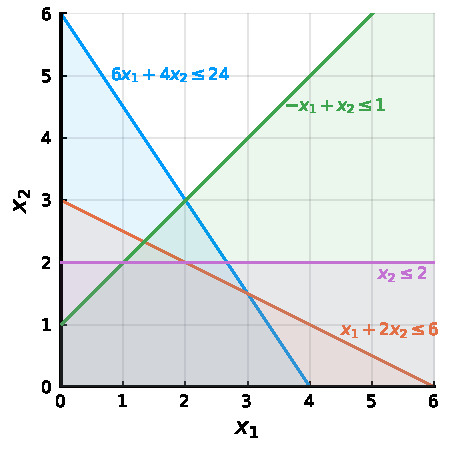
\includegraphics[scale=0.9]{chapters/chapter_1/figures/figure1-3a.pdf}	
		\caption{} \label{c1:fig:fig3a}
	\end{subfigure}
	\begin{subfigure}{0.49\textwidth}
		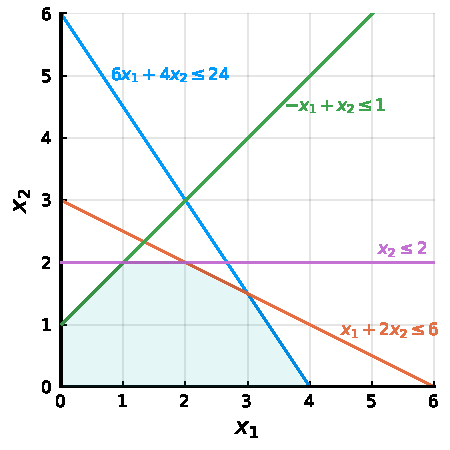
\includegraphics[scale=0.9]{chapters/chapter_1/figures/figure1-3b.pdf}
		\caption{} \label{c1:fig:fig3b}		
	\end{subfigure}
	\caption{The feasible region of the paint factory problem (in Figure \ref{c1:fig:fig3b}), represented as the intersection of the four closed-half spaces formed by each of the constraints (as shown in Figure \ref{c1:fig:fig3a}). Notice how the feasible region is a polyhedral set in $\reals^2$, as there are two decision variables ($x_1$ and $x_2$)} \label{c1:fig:feasible_region_plot}	
\end{figure}

We can use this visual representation to find the optimal solution for the problem, that is, the point $(x_1,x_2)$ within the feasible set such that the objective function value is maximal (recall that the paint factory problem is a maximisation problem). For that, we must consider how the objective function $z = c^\top x$ can be represented in the $(x_1, x_2)$-plane. Notice that the objective function forms a hyperplane in $(x_1, x_2, z) \subset \reals^3$, of which we can plot level curves (i.e., projections) onto the $(x_1, x_2)$-plane. Figure \ref{c1:fig:level_curves_a} shows the plotting of three level curves, for $z= 5, 10$, and $15$. 

This observation provides us with a simple graphical method to find the optimal solution to linear problems. One must simply \emph{sweep} the feasible region in the direction of the gradient $\nabla z=[\frac{\partial z}{\partial x_1},\frac{\partial z}{\partial x_2}]^\top=[5,4]^\top$ (or in its opposite direction, if minimising) until one last point (or edge) of contact remains, meaning that the whole of the feasible region is behind that furthermost level curve. Figure \ref{c1:fig:level_curves_b} illustrates the process of finding the optimal solution for the paint factory problem.

\begin{figure}[H]
	\begin{subfigure}{0.49\textwidth}
		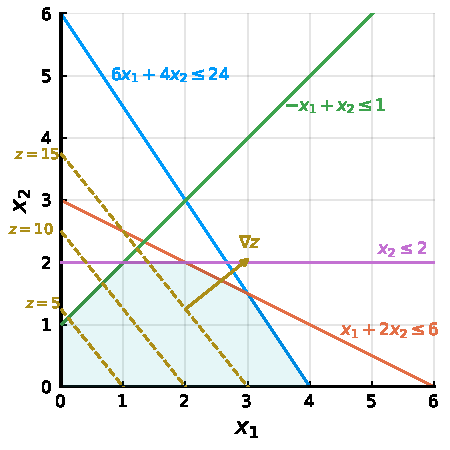
\includegraphics[scale=0.9]{chapters/chapter_1/figures/figure1-4a.pdf}  
		\caption{} \label{c1:fig:level_curves_a}	
	\end{subfigure}
	\begin{subfigure}{0.49\textwidth}
		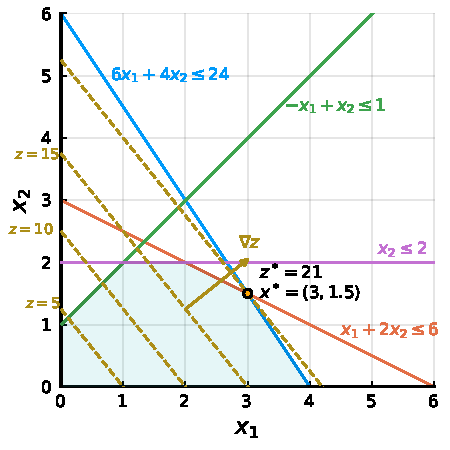
\includegraphics[scale=0.9]{chapters/chapter_1/figures/figure1-4b.pdf}
		\caption{} \label{c1:fig:level_curves_b}	 
	\end{subfigure}
	\caption{Graphical representation of some of the level curves of the objective function $z = 5x_1 + 4x_2$. Notice that the constant gradient vector $\nabla z = (5,4)^\top$ points to the direction in which the level curves increase in value. The optimal point is represented by $x^*=(3, 1.5)^\top$ with the furthermost level curve being that associated with the value $z^* = 21$}	
\end{figure}

The graphical method is important because it allows us to notice several key features that will be used later on when we analyse a method that can search for optimal solutions for LP problems. The first is related to the notion of active or inactive constraints. We say that a constraint is \emph{active} at a given point $x$ if the constraint is satisfied as equality at the point $x$. For example, the constraints $6x_1 + 4x_2 \leq 24$ and $x_1 + 2x_2 \leq 6$ are active at the optimum $x^* = (3, 1.5)$, since $6(3) + 4(1.5) = 24$ and $3 + 2(1.5) = 6$. An active constraint indicates that the resource (or requirement) represented by that constraint is being fully depleted (or minimally satisfied). 

Analogously, \emph{inactive constraints} are constraints that are satisfied as strict inequalities at the optimum. For example, the constraint $-x_1 + x_2 \leq 1$ is inactive at the optimum, as $-(3) + 1.5 < 1$. In this case, an inactive constraint represents a resource (or requirement) that is not fully depleted (or is over-satisfied).


\subsection{Geometrical properties of LPs}

One striking feature concerning the geometry of LPs that becomes evident when we analyse the graphical method is that the number of candidate solutions is not infinite, but instead, only \emph{a finite set} of points are potential candidates for optimal solution. This is because the process of sweeping in the direction of the gradient of the (linear) objective function will, in general, lead to a unique solution that must lie on a vertex of the polyhedral feasible set. The only exceptions are either when the gradient $\nabla z$ happens to be perpendicular to a facet of the polyhedral set (and in the direction of the sweeping) or in case the sweeping direction is not bounded by some of the facets of the polyhedral set. These exceptional cases will be discussed in more detail later on, but, as we will see, the observation still holds.

In the graphical example (i.e., in $\reals^2$), notice how making $n = 2$ constraints active out of $m = 4$ constraints \emph{forms a vertex}. However, not all vertices are feasible. This allows us to devise a mechanism to describe vertices by activating $n$ of the $m$ constraints at a time, in which we could exhaustively test and select the best (i.e., that with the largest objective function value). The issue, however, is that the number of candidates increases \emph{exponentially} with the number of constraints and variables of the problem, which indicates this would quickly become computationally infeasible. As we will see, it turns out that this search idea can be made surprisingly efficient and is, in fact, the underlying framework of the \emph{simplex method}. However, there are indeed artificially engineered worst-case settings where the method does need to consider every single vertex.

The simplex method exploits the above idea to \emph{heuristically} search for solutions by selecting $n$ constraints to be active from the $m$ constraints available. Starting from an initial selection of constraints to be active, it selects one inactive constraint to activate and one to deactivate in a way that improvement in the objective function can be observed while feasibility is maintained. This process repeats until no improvement can be observed. In such a case, the \emph{geometry} of the problem guarantees \emph{(global) optimality}. In the following chapters, we will concentrate on defining algebraic objects that we will use to develop the simplex method.


\vfill
\pagebreak

\section{Exercises}

\subsection*{Exercise 1.1: Introduction to JuMP}
Use the Julia package JuMP.jl to implement the problems below and find the optimal solution. For the two-dimensional problems, use Plots.jl to illustrate the feasible region and the optimal solution.

\begin{enumerate}
	\item[(a)]
		\begin{flalign*}
			\maxi & x_1 + 2x_2 + 5x_3 &&\\
			\st   & x_1 - x_2 - 3x_3 \geq 5 &&\\
				  & x_1 + 3x_2 - 7x_3 \leq 10 &&\\
				  & x_1 \leq 10 &&\\
				  & x_1, x_2 \geq 0. &&
		\end{flalign*}

	\item[(b)]
		\begin{flalign*}
			\maxi & 2x_1 + 4x_2 &&\\
			\st   & x_1 + x_2 \leq 5 &&\\
			  	  & -x_1 + 3x_2 \leq 1 &&\\
	  			  & x_1 \leq 5 &&\\
				  & x_2 \leq 5 &&\\
				  & x_1, x_2 \geq 0. &&
		\end{flalign*}
	
	\item[(c)]
		\begin{flalign*}			
			\mini & -5x_1 + 10x_2 + x_3 + 2000x_4 &&\\
			\st   &  x_1 - x_2 \leq 1500 &&\\
				  & 4x_2 - x_3 \leq 5000x_4 &&\\
				  & x_1 + 3x_2 \geq 1000 &&\\
				  & x_1  \leq 10000 &&\\
				  & x_1, x_2 \in \reals, x_3 \leq 0, x_4 \in \braces{0,1}. &&
		\end{flalign*}

	\item[(d)]
		\begin{flalign*}	
			\maxi & 5x_1 + 3x_2 &&\\
			\st   & x_1 + 5x_2 \leq 3 &&\\
				  & 3x_1 - x_2 \leq 5 &&\\
				  & x_1 \leq 2 &&\\
 				  & x_2 \leq 30 &&\\
				  & x_1, x_2 \geq 0. &&
		\end{flalign*}
\end{enumerate}




\subsection*{Exercise 1.2: Transportation problem \cite{kwon2019julia}}
Consider the following network, where the supplies from the Austin and Buffalo nodes need to meet the demands in Chicago, Denver, and Erie. The data for the problem is presented in table below.

\begin{figure}[h]
	\begin{tikzpicture}[scale=1,
		node/.style={circle, fill=blue!40, draw, minimum size=3em, inner sep=1pt},
		node2/.style={circle, fill=orange, draw, minimum size=3em, inner sep=1pt}] 
    	\node[above] at (0, 4.75) {Plants};                                                                                  
    	\node[above] at (3, 4.75) {Clients};
	    \node[node] (1) at (0, 2) {\footnotesize Austin};
	    \node[node] (2) at (0, 3.5) {\footnotesize Buffalo};
	    \node[node2] (3) at (3, 4) {\footnotesize Chicago};
	    \node[node2] (4) at (3, 2.5) {\footnotesize Denver};
	    \node[node2] (5) at (3, 1) {\footnotesize Erie};
	    \foreach \x in {1,...,2} {
	       \foreach \y in {3,...,5} {
	          \draw[->, thick] (\x) -- (\y);
	          }}      
	\end{tikzpicture}
\end{figure}

\begin{table}[h]
	\begin{tabular}{r|ccc|c}
    	& & {\it Clients} &\\\hline
    	{\it Factory} & Chicago & Denver & Eire \\\hline
    	Buffalo 		  & 4       & 9      & 8    & 25 \\
    	Austin        & 10      & 7      & 9    & 600 \\\hline
    	Demands       & 15      & 12     & 13   & - \\\hline
	\end{tabular}
	\caption{Problem data: unit transportation costs, demands and capacities}
\end{table}

Solve the transportation problem, finding the minimum cost transportation plan.


\subsection*{Exercise 1.3: Capacitated transportation}
The Finnish company Next has a logistics problem in which used oils serve as raw material to form a class of renewable diesel. The supply chain team need to organise, to a minimal cost, the acquisition of two types of used oils (products p1 and p2) from three suppliers (supply nodes s1, s2, and s3) to feed the line of three of their used oils processing factories (demand nodes d1, d2, and d3). As the used oils are the byproduct of the supplier's core activities, the only requirement is that Next need to fetch the amount of oil and pay the transportation costs alone.

The oils have specific conditioning and handling requirements, so transportation costs vary between p1 and p2. Additionally, not all the routes (arcs) between suppliers and factories are available as some distances are not economically feasible. Table \ref{p1c1:tab:ex1-4_suplly_demand} shows the volume requirement of the two types of oil from each supply and demand node, and table \ref{p1c1:tab:ex1-4_arcs} show the transportation costs for each oil type per L and the arc capacity. Arcs with ``-'' for costs are not available as transportation routes.

\begin{table}[h!]
	\begin{subtable}[h]{0.4\textwidth}
		\begin{center}
		\begin{tabular}{c|cc}
			\textbf{node} & \textbf{p1} & \textbf{p2} \\
			\hline
			\textbf{s1 / d1} & 80 / 60 & 400 / 300 \\
			\textbf{s2 / d2} & 200 / 100 & 1500 / 1000 \\
			\textbf{s3 / d3} & 200 / 200 & 300 / 500 \\
		\end{tabular}
		\end{center}
		\caption{Supply availability and demand per oil type [in L]}
		\label{p1c1:tab:ex1-4_suplly_demand}
	\end{subtable}
	\hfill
	\begin{subtable}[h]{0.55\textwidth}
		\begin{center}
			\begin{tabular}{c|ccc}
				 & \textbf{d1} & \textbf{d2} & \textbf{d3}\\
				 & \textbf{p1/p2 (cap)} & \textbf{p1/p2 (cap)} & \textbf{p1/p2 (cap)}\\
				\hline
				\textbf{s1} & 5/- ($\infty$) & 5/18 (300) & -/- (0)\\
				\textbf{s2} & 8/15 (300) & 9/12 (700) & 7/14 (600)\\
				\textbf{s3} & -/- (0) & 10/20 ($\infty$) & 8/- ($\infty$)\\
			\end{tabular}
		\end{center}
		\caption{Arcs costs per oil type [in \euro \ per L] and arc capacities [in L]}
		\label{p1c1:tab:ex1-4_arcs}
	\end{subtable}
	\caption{Supply chain data}
\end{table}

Find the optimal oil acquisition plan for Next, i.e., solve its transportation problem to the minimum cost.


\subsection*{Exercise 1.4: The farmer's problem \cite{birge2011introduction}}
Consider a farmer who produces wheat, corn, and sugar beets on his 500 acres of land. During the winter, the farmer wants to decide 
how much land to devote to each crop. 

The farmer knows that at least 200 tons (T) of wheat and 240T of corn are needed for cattle feed. 
These amounts can be raised on the farm or bought from a wholesaler. Any production in excess of the feeding requirement would be sold. Over the last decade, mean selling prices have been \$ 170 and \$ 150 per ton of wheat and corn, respectively. The purchase prices are 40 \% more than this due to the wholesaler's margin and transportation costs. The planting costs per acre of wheat and corn are \$ 150 and \$ 230, respectively.

Another profitable crop is sugar beet, which he expects to sell at \$36/T; however, the European Commission imposes a quota on sugar beet 
production. Any amount in excess of the quota can be sold only at \$10/T. The farmer’s quota for next year is 6000T. The planting cost per acre of sugar beet is \$ 260.

Based on past experience, the farmer knows that the mean yield on his land is
roughly 2.5T, 3T, and 20T per acre for wheat, corn, and sugar beets, respectively.

Based on the data, build up a model to help the farmer allocate the farming area to each crop and how much to sell/buy of wheat, corn, 
and sugar beets considering the following cases.

\begin{itemize}
	\item[(a)] The predictions are 100\% accurate and the mean yields are the only realizations possible.	
	\item[(b)] There are three possible equiprobable scenarios (i.e, each one with a probability equal to $\frac{1}{3}$): a good, fair, and bad weather scenario. In the good weather, the yield is 20\% better than the yield expected whereas in the bad weather scenario it is reduced 20\% of the mean yield. In the regular weather scenario, the yield for each crop keeps the historical mean - 2.5T/acre, 3T/acre, and 20T/acre for wheat, corn, and sugar beets, respectively.
	\item[(c)]	What happens if we assume the same scenarios as item (b) but with probabilities 25\%, 25\%, and 50\% for good, fair, and bad weather, respectively? How the production plan changes and why?	
\end{itemize}


\subsection*{Exercise 1.5: Factory planning \cite{williams2013model}}
A factory makes seven products (PROD 1 to PROD 7) using the
following machines: four grinders, two vertical drills, three horizontal drills, one
borer and one planer. Each product yields a certain contribution to the profit (defined
as \$/unit selling price minus the cost of raw materials). These quantities (in \$/unit)
together with the unit production times (hours) required on each process are given
in Table \ref{p1c1:tab:ex1-5_prod_yield}. A dash indicates that a product does not require a process. 
There are also marketing demand limitations on each product each month. These are given in Table \ref{p1c1:tab:ex1-5_max_demand}.

\begin{table}[h]
	\begin{tabular}{l|lllllll}
		& \textbf{PROD1} & \textbf{PROD2} & \textbf{PROD3} & \textbf{PROD4} & \textbf{PROD5} & \textbf{PROD6} & \textbf{PROD7} \\ \hline 
		\textbf{Profit} & 10    & 6     & 8     & 4     & 11    & 9     & 3     \\
		\textbf{Grinding}              & 1.5   & 2.1   & –     & –     & 0.9   & 0.6   & 1.5   \\
		\textbf{Vert. drilling}     & 0.3   & 0.6   & –     & 0.9   & –     & 1.8   & –     \\
		\textbf{Horiz. drilling}   & 0.6   & –     & 2.4   & –     & –     & –     & 1.8   \\
		\textbf{Boring}                & 0.15  & 0.09  & –     & 0.21  & 0.3   & –     & 0.24  \\
		\textbf{Planing}               & –     & –     & 0.03  & –     & 0.15  & –     & 0.15 \\ \hline
	\end{tabular}
	\caption{Product yields}
	\label{p1c1:tab:ex1-5_prod_yield}
\end{table}

\begin{table}[H]
	\begin{tabular}{l|lllllll}
		& \textbf{PROD1} & \textbf{PROD2} & \textbf{PROD3} & \textbf{PROD4} & \textbf{PROD5} & \textbf{PROD6} & \textbf{PROD7} \\ \hline
		\textbf{January}   & 500   & 1000  & 300   & 300   & 800   & 200   & 100   \\
		\textbf{February}  & 600   & 500   & 200   & 0     & 400   & 300   & 150   \\
		\textbf{March}     & 300   & 600   & 0     & 0     & 500   & 400   & 100   \\
		\textbf{April}     & 200   & 300   & 400   & 500   & 200   & 0     & 100   \\
		\textbf{May}       & 0     & 100   & 500   & 100   & 1000  & 300   & 0     \\
		\textbf{June}      & 500   & 500   & 100   & 300   & 1100  & 500   & 60    \\ \hline
	\end{tabular}
	\caption{Maximum demand}
	\label{p1c1:tab:ex1-5_max_demand}
\end{table}

It is possible to store up to 100 of each product at a time at a cost of \$0.5 per unit per month. There are no stocks at present, but it is desired to have a stock of 50 of each type of product at the end of June. 

The factory works six days a week with two shifts of 8h each day. Assume that each month consists of only 24 working days. Also, there are no penalties for unmet demands. What is the factory's production plan (how much of which product to make and when) in order to maximise the total profit?



\subsection*{Exercise 1.6: Linear classifier}
Suppose we have a set of pre-classified data points $x_i$ in $\mathbb{R}^n$, divided into two sets based on their classification. For example, the data could be information on patients and the two sets would correspond to patients who have or do not have a certain disease. Note that unlike so far, $x$ is now data, not a decision variable. Denote the respective index sets by $I_1$ and $I_2$, respectively. In order to predict the class of a new point $x_{new}$, we want to infer a classification rule from the data.
\begin{figure}
    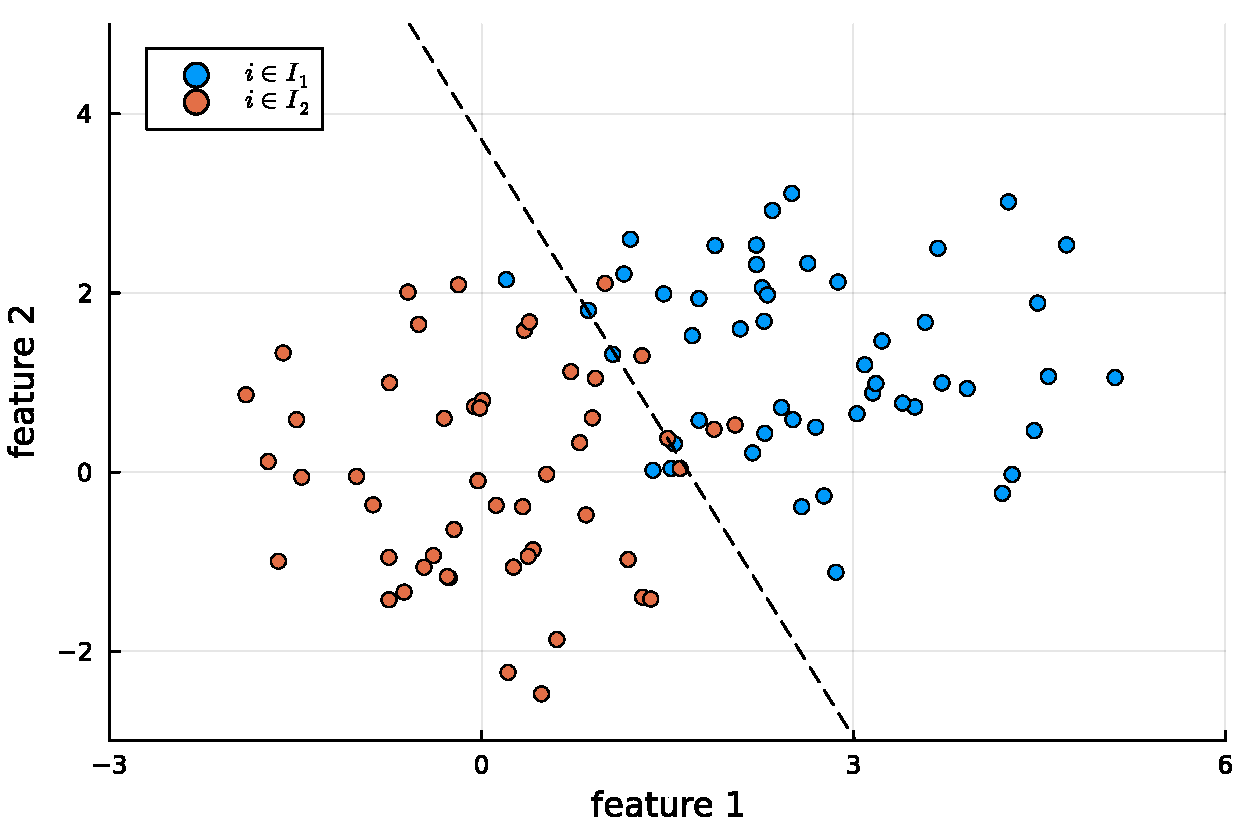
\includegraphics[width=0.75\textwidth]{chapters/chapter_1/figures/figure_e16.pdf}
    \caption{Two sets of data points defined by two features, separated by a line $ax=b$} 
    \label{p1c1:fig:fig_e16}		
\end{figure}

Write a linear programming problem that finds the hyperplane $ax = b$ such that if $ax_{new} > b$, the point $x_{new}$ is predicted to be in class 1, and if $ax_{new}<b$, the predicted class is 2. The hyperplane should be optimal in the sense that it minimizes the sum of absolute deviations $|ax_i-b|$ for the misclassified points $x_i$ in the training data, that is, points on the wrong side of the hyperplane. In Fig. \ref{p1c1:fig:fig_e16}, any red point $x_i$, $i \in I_2$ that is on the top/right of the line is on the wrong side and thus accumulates the error, and similarly for blue points on the bottom/left of the line.





	
	\chapter{Basics of Linear Algebra} \label{chapter_2}
	\section{Basics of linear problems}


%TODO: Chp2: It would be more natural to start with the convexity of polyhedral sets and then move on to the linear algebra definitions. We just need to be careful to define the elements needed (halfspaces, hyperplanes, etc) so the presentation of convexity elements make sense 

As we have seen in the previous chapter, the feasible region of a linear programming problem can be represented as
%
\begin{equation} \label{p1c2:eq:feasible_region_inequality}
	Ax \leq b,	
\end{equation}

where $A$ is a $m \times n$ matrix, $x$ is a $n$-dimensional column vector (or more compactly, $x \in \reals^n$), and $b$ is an $m$-dimensional column vector ($b \in \reals^m$). Notice that $\leq$ is considered component-wise. Also, let $\dim(x)$ denote the dimension of vector $x$.

Before introducing the simplex method, let us first revisit a few key elements and operations that we will use in the process. The first of them is presented in Definition \ref{p1c2:def:matrix_inversion}.
%
\begin{definition}[Matrix inversion] \label{p1c2:def:matrix_inversion}
	Let $A$ be a square $n \times n$ matrix. $A^{-1}$ is the inverse matrix of $A$ if it exists and $AA^{-1} = I$, where  $I$ is the ($n \times n$) identity matrix.
\end{definition}
%
Matrix inversion is the ``kingpin'' of linear (and nonlinear) optimisation. As we will see later on, performing efficient matrix inversion operations (in reality, operations that are equivalent to matrix inversion but that can exploit the matrix structure to be made faster) is of utmost importance for developing a linear optimisation solver. 

Another important concept is the notion of \emph{linear independence}. We formally state when a collection of vectors is said to be linearly independent (or dependent) in Definition \ref{p1c2:def:linear_independence}. 

%
\begin{definition}[Linearly independent vectors] \label{p1c2:def:linear_independence}
	The vectors $\braces{x_i}_{i=1}^k \in \reals^n$  are linearly dependent if there exist real numbers $\braces{a_i}_{i=1}^k$ with $a_i \neq 0$ for at least one $i \in \braces{1,\dots, k}$ such that
	$$
		\sum_{i=1}^k a_i x_i= 0;
	$$
	otherwise, $\braces{x_i}_{i=1}^k$ are linearly independent.
\end{definition}

In essence, for a collection of vectors to be linearly independent, it must be so that none of the vectors in the collection can be expressed as a linear combination (that is, multiplying the vectors by nonzero scalars and adding them) of the others. Analogously, they are said to be linearly dependent if one vector in the collection can be expressed as a linear combination of the others. 

This is simpler to see in $\reals^2$. Two vectors are linearly independent if one cannot obtain one by multiplying the other by a constant, which effectively means that they are not parallel. If the two vectors are not parallel, then one of them must have a component in a direction that the other vector cannot ``reach''. The same idea can be generalised to any $n$-dimensional space. Also, that explains why one can only have up to $n$ independent vectors in $\reals^n$. Figure \ref{p1c2:fig:linear_independence} illustrates this idea. 

\begin{figure}[h]
	\centering
    \begin{tikzpicture}
%	    \draw[help lines] (-2,-2) grid (2,3);
		\node (pic) at (0,0) {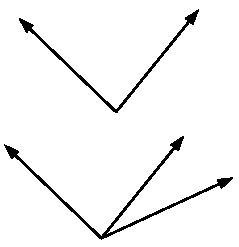
\includegraphics{chapters/chapter_2/figures/Figure1}};
		\node (x1) at (-1.7, 2.1) {$x_1$};
		\node (x2) at (1.2, 2.2) {$x_2$};
		\node (x11) at (-1.9, -0.2) {$x_1$};
		\node (x12) at (1, 0) {$x_2$};
		\node (x3) at (2.1, -0.8) {$x_3$};
    \end{tikzpicture}
	\caption{Linearly independent (top) and dependent (bottom) vectors in $\reals^2$. Notice how, in the bottom picture, any of the vectors can be obtained by appropriately scaling and adding the other two}\label{p1c2:fig:linear_independence}
\end{figure}

Theorem \ref{p1c2:thm:fundamental_linear_algebra} summarises results that we will utilise in the upcoming developments. These are classical results from linear algebra and the proof is left as an exercise.
%
\begin{theorem}[Inverses, linear independence, and solving $Ax = b$] \label{p1c2:thm:fundamental_linear_algebra}
	Let $A$ be a $m \times m$ matrix. Then, the following statements are equivalent:
	\begin{enumerate}
		\item $A$ is invertible
		\item $A^\top$ is invertible
		\item The determinant of $A$ is nonzero
		\item The rows of $A$ are linearly independent
		\item The columns of $A$ are linearly independent
		\item For every $b \in \reals^m$, the linear system $Ax = b$ has a unique solution
		\item There exists some $b \in \reals^m$ such that $Ax = b$ has a unique solution.	
	\end{enumerate}	
\end{theorem}
%
Notice that Theorem \ref{p1c2:thm:fundamental_linear_algebra} establishes important relationships between the geometry of the matrix $A$ (its rows and columns) and consequences it has to our ability to calculate its inverse $A^{-1}$ and, consequently, solve the system $Ax = b$, to which the solution is obtained as $x = A^{-1}b$. Solving linear systems of equations will turn out to be the most important operation in the simplex method.


\subsection{Subspaces and bases}

Let us define some objects that we will frequently refer to. The first of them is the notion of a \emph{subspace}. A subspace of $\reals^n$ is a set comprising all linear combinations of its own elements. Specifically, if $S$ is a subspace, then
%
\begin{equation*}
	S = \braces{ax + by : x,y \in S; a,b \in \reals}.
\end{equation*}
%
A related concept is the notion of a \emph{span}. A span of a collection of vectors $\braces{x_i}_{i=1}^k \in \reals^n$ is the subspace of $\reals^n$ formed by all linear combinations of such vectors, i.e., 
%
\begin{equation*}
	\spans(x_1,\dots, x_k) = \braces{y = \sum_{i=1}^k a_ix_i : a_i \in \reals, i \in \braces{1,\dots, k}}. 
\end{equation*}
%
Notice how the two concepts are related: the span of a collection of vectors forms a subspace. Therefore, a subspace can be characterised by the collection of vectors whose span forms it. In other words, the span of a set of vectors is the subspace formed by all points we can represent by some linear combination of these vectors. 

The missing part in this is the notion of a \emph{basis}. A \emph{basis} of the subspace $S \subseteq \reals^n$ is a collection of vectors $\braces{x_i}_{i=1}^k \in \reals^n$ that are linearly independent such that $\spans(x_1,\dots, x_k) = S$. 

Notice that a basis is a ``minimal'' set of vectors that form a subspace. You can think of it in light of the definition of linearly independent vectors (Definition \ref{p1c2:def:linear_independence}); if a vector is linearly dependent to the others, it is not needed for characterising the subspace that the vectors span since it can be represented by a linear combination of the other vectors (and thus is in the subspace formed by the span of the other vectors).

The above leads us to some important realisations:

\begin{enumerate}
	\item All bases of a given subspace $S$ have the same dimension. Any extra vector would be linearly dependent to those vectors that span $S$. In that case, we say that the subspace has size (or dimension) $k$, the number of linearly independent vectors forming the basis of the subspace. We can overload the notation $\dim(S)$ to represent the dimension of the subspace $S$.
	\item If the subspace $S \subset \reals^n$ is formed by a basis of size $m < n$, we say that $S$ is a proper subspace with $\dim(S)=m$, because it is not the whole $\reals^n$ itself, but a space contained within $\reals^n$. For example, two linearly independent vectors form (i.e., span) a hyperplane in $\reals^3$; this hyperplane is a proper subspace since $\dim(S)=m=2 < 3=n$.
	\item If a proper subspace has dimension $m < n$, then it means that there are $n-m$ directions in $\reals^n$ that are perpendicular to the subspace and to each other. That is, there are nonzero vectors $a_i$ that are orthogonal to each other and to $S$. Or, equivalently, $a_i^\top x = 0$ for $i = n-m + 1, ..., n$. Referring to the $\reals^3$, if $m=2$, then there is a third direction that is perpendicular to (or not in) $S$. Figure \ref{p1c2:fig:proper_subpaces} can be used to illustrate this idea. Notice how one can find a vector, say $x_3$ that is perpendicular to $S$. This is because the whole space is $\reals^3$, but $S$ has dimension $m=2$ (or $\dim(S)=2$). 
\end{enumerate}

\begin{figure}
	\centering
	\begin{tikzpicture}
%			\draw[help lines] (-4,-2) grid (4,2);
		\node (pic) at (0,0) {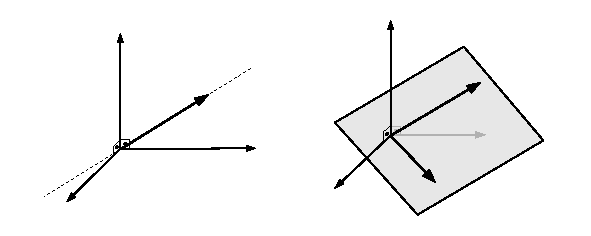
\includegraphics{chapters/chapter_2/figures/Figure2}};
		\node (x1l) at (-1.6, 0.6) {$x_1$};
		\node (Sl) at (-1.1, 0.9) {$S$};	
		\node (x1r) at (2.8, 0.8) {$x_1$};
		\node (x2r) at (2.6, -0.9) {$x_2$};
		\node (Sr) at (3.7, -0.3) {$S$};
	\end{tikzpicture}
	\vspace{-12pt}
	\caption{One- (left) and two-dimensional subspaces (right) in $\reals^3$.} \label{p1c2:fig:proper_subpaces}
\end{figure}

Theorem \ref{p1c2:thm:LI_and_bases} builds upon the previous points to guarantee the existence of bases and propose a procedure to form them.

\begin{theorem}[Forming bases from linearly independent vectors]\label{p1c2:thm:LI_and_bases}
	Suppose that $S = \spans(x_1,\dots, x_k)$ has dimension $m \leq k$. Then
	\begin{enumerate}
		\item There exists a basis of $S$ consisting of $m$ of the vectors $x_1,\dots, x_k$.
		\item If $k' \leq m$ and $x_1,\dots, x_{k'} \in S$ are linearly independent, we can form a basis for $S$ by starting with $x_1,\dots, x_{k'}$ and choosing $m-{k'}$ additional vectors from $x_1,\dots, x_k$.
	\end{enumerate}	
\end{theorem}

\begin{proof}
	Notice that, if every vector $x_{k'+1}, \dots, x_{k}$ can be expressed as a linear combination of $x_{1},\dots x_{k'}$, then every vector in $S$ is also a linear combination of $x_{1}, \dots, x_{k'}$. Thus, $x_{1}, \dots, x_{k'}$ form a basis to $S$ with $m =k'$. Otherwise, at least one of the vectors in $x_{k'+1}, \dots, x_{k}$ is linearly independent from $x_{1}, \dots, x_{k'}$. By picking one such vector, we now have $k'+1$ of the vectors $x_{k'+1}, \dots, x_{k}$ that are linearly independent. If we repeat this process $m - k'$ times, we end up with a basis for $S$.
\end{proof}


Our interest in subspaces and bases spans (pun intended!) from their usefulness in explaining how the simplex method works under a purely algebraic (as opposed to geometric) perspective. For now, we can use the opportunity to define some ``famous'' subspaces which will often appear in our derivations. 

Let $A$ be a $m \times n$ matrix. The \emph{column space} of $A$ consists of the subspace spanned by the $n$ columns of $A$ and has dimension $m$ (recall that each column has as many components as the number of rows and is thus a $m$-dimensional vector). Likewise, the \emph{row space} of $A$ is the subspace in $\reals^n$ spanned by the rows of $A$. Finally, the \emph{null space} of $A$, often denoted as $\nulls(A) = \braces{x \in \reals^n : Ax = 0}$, consist of the vectors that are perpendicular to the row space of $A$. 

One important notion related to those subspaces is their size. Both the row and the column space have the same size, which is the \emph{rank} of $A$. If $A$ is \emph{full rank}, than it means that 
%
\begin{equation*}
	\rank(A) = \min \braces{m,n}. 		
\end{equation*}
%
Finally, the size of the null space of $A$ is given $n - \rank(A)$, which is in line with Theorem \ref{p1c2:thm:LI_and_bases}.


\subsection{Affine subspaces}

A related concept is that of an \emph{affine subspace}. Differently from linear subspaces (to which we have been referring to simply as subspaces), affine subspaces encode some form of translation, such as  
%
\begin{equation*}
	S = S_0 + x_0 = \braces{x + x_0 : x \in S_0}.
\end{equation*}
%
Affine subspaces differ from linear subspaces because they do not contain the origin (recall that the definition of subspaces allows for $a$ and $b$ to be zero). Nevertheless, $S$ has the \emph{same dimension} as $S_0$.

Affine subspaces give a framework for representing linear programming problems algebraically. Specifically, let $A$ be a $m \times n$ matrix with $m < n$ and $b$ a $m$-dimensional vector. Then, let 
%
\begin{equation} \label{p1c2:eq:equality_constraint_feasible_set}
	S = \braces{x \in \reals^n : Ax = b}.		
\end{equation}
%
As we will see, the feasible set of any linear programming problem can be represented as an equality-constrained equivalent of the form of \eqref{p1c2:eq:equality_constraint_feasible_set} by adding slack variables to the inequality constraints, meaning that we will always have that $m < n$.  Now, assume that $x_0 \in \reals^n$ is such that $Ax_0 = b$.  Then, we have that 
%
\begin{equation*}
	Ax = Ax_0 = b \Rightarrow A(x - x_0) = 0.	
\end{equation*}
%
Thus, $x \in S$ if and only if the vector $(x - x_0)$ belongs to $\nulls(A)$, the nullspace of $A$. Notice that the feasible region $S$ can be also defined as 
%
\begin{equation*}
	S = \braces{x + x_0 : x \in \nulls(A)},	
\end{equation*}
%
being thus an affine subspace with dimension $n-m$, if $A$ has $m$ linearly independent rows (i.e., $\rank(A)=m$). This will have important implications in the way we can define multiple bases for $S$ from the $n$ vectors in the column space and what implications it has for the feasibility of the whole problem. Figure \ref{p1c2:fig:nill_space_a} illustrates this concept for a single-row matrix $a$. For a multiple-row matrix $A$, $S$ becomes the intersection of multiple hyperplanes.

\begin{figure}
	\begin{tikzpicture}
	    \node (pic) at (0,0) {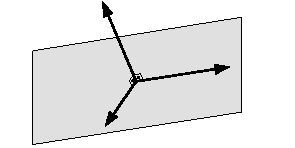
\includegraphics{chapters/chapter_2/figures/Figure3}};
	    \node (x0) at (0,-0.4) {$x_0$};
	    \node (x1) at (1.4,0.4) {$x_1$};
	    \node (x2) at (-1,-0.9) {$x_2$};
	    \node (a) at (-0.5,1.4) {$a$};
	    \node (S) at (-1.7,0.2) {$S$}; 
	\end{tikzpicture}
	\caption{The affine subspace $S$ generated by $x_0$ and $\nulls(a)$. Notice that all vectors in $S$, exemplified by $x_1$ and $x_2$ are perpendicular (i.e., have null dot product) to $a$} \label{p1c2:fig:nill_space_a}.		
\end{figure}


\section{Convex polyhedral set}

The feasible region of any linear programming problem is a convex polyhedral set, which we will simply refer to as a polyhedral set. That is because we are interested in polyhedral sets that are formed by an intersection of a finite number of half-spaces and can thus only be convex (as we will see in a moment), creating redundancy in our context but maybe some confusion overall. 

\subsection{Hyperplanes, half-spaces and polyhedral sets}

Definition \ref{p1c2:def:polyhedral_sets} formally states the structure that we refer to as polyhedral sets.
%
\begin{definition}[Polyhedral set] \label{p1c2:def:polyhedral_sets}
	A polyhedral set is a set that can be described as
	$$
	S = \braces{x \in \reals^n : Ax \geq b},	
	$$
	where $A$ is an $m \times n$ matrix and $b$ is a $m$-vector.
\end{definition}
%
One important thing to notice is that polyhedral sets, as defined in Definition \ref{p1c2:def:polyhedral_sets}, as formed by the intersection multiple half-spaces. Specifically, let $\braces{a_i}_{i=1}^m$ be the rows of $A$. Then, the set $S$ can be described as 
%
\begin{equation}
	S = \braces{x \in \reals^n : a_i^\top x \geq b_i, i = 1,\dots, m}, 	
\end{equation}
%
which represents exactly the intersection of the half-spaces $a_i^\top x \geq b_i$. Furthermore, notice that the hyperplanes $a_i^\top x = b_i$, $\forall i \in \braces{1,\dots, m}$, are the boundaries of each hyperplane, and thus describe one of the facets of the polyhedral set. Figure \ref{p1c2:fig:hyperplanes_and_polyhedral_set} illustrates a hyperplane forming two half-spaces (also polyhedral sets) and how the intersection of five half-spaces form a (bounded) polyhedral set.

\begin{figure}[h]
			\begin{tikzpicture}
		    \node (pic) at (0,0) {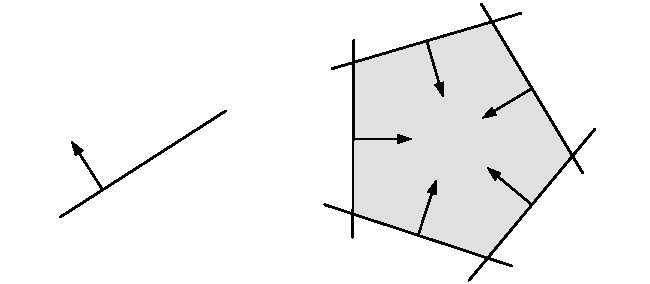
\includegraphics{chapters/chapter_2/figures/Figure4}};
		    \node (a) at (-4.5,0.2) {$a$};
			\node (ax=b) at (-3.6,-1.3) {$a^\top x =b$};
			\node (ax<b) at (-2.5, 0.8) {$a^\top x > b$};
			\node (ax>b) at (-2.3,-0.7) {$a^\top x < b$};
			\node (a1) at (1.5, -0.2) {$a_1$};
			\node (a2) at (2.8, 0.2) {$a_2$};
			\node (a3) at (1.8, 0.7) {$a_3$};
			\node (a4) at (2.9, -0.3) {$a_4$};
			\node (a5) at (2.2, -0.8) {$a_5$};
			\node[rotate = 90] (a1x=b1) at (0.1,0.2) {$a_1^\top x =b_1$};
			\node (a3x=b3) at (1.5,2.2) {$a_3^\top x =b_3$};
			\node (a2x=b2) at (4.5, 1) {$a_2^\top x =b_2$};
			\node (a4x=b4) at (4.4,-1.2) {$a_4^\top x =b_4$};
			\node (a5x=b5) at (1.3,-2) {$a_5^\top x =b_5$};
			\end{tikzpicture}
			\vspace{1pt}
		\caption{A hyperplane and its respective halfspaces (left) and the polyhedral set $\braces{x\in \reals^{2} : a_i^x \geq b_i, i =1,\dots, 5}$ (right).} \label{p1c2:fig:hyperplanes_and_polyhedral_set}		
	\end{figure}

You might find authors referring to bounded polyhedral sets as polytopes. However, this is not used consistently across references, sometimes with switched meanings (for example, using polytope to refer to a set defined as in Definition \ref{p1c2:def:polyhedral_sets} and using polyhedron to refer to a bounded version of $S$). In this text, we will only use the term polyhedral set to refer to sets defined as in Definition \ref{p1c2:def:polyhedral_sets} and use the term bounded whenever applicable.

Also, it may be useful to formally define some elements in polyhedral sets. For that, let us consider a hyperplane $H = \braces{x \in \reals^{n} : a^\top x = b}$, with $a \in \reals^n$ and $b \in \reals$. Now consider the set $F = H \cap S$. This set is known as a \emph{face} of a polyhedral set. If the face $F$ has dimension zero, then $F$ is called a vertex. Analogously, if $\dim(F)=1$, then $F$ is called an edge. Finally, if $\dim(F) = dim(S)-1$, then $F$ is called a facet. Notice that in $\reals^3$, facets and faces are the same, whenever the face is not an edge or a vertex. 


\subsection{Convexity of polyhedral sets}

As will see in more detail in Part 2 of this book, convexity plays a crucial role in optimisation, being the ``watershed'' between easy and hard optimisation problems. One of the main reasons why we can solve challenging linear programming problems is due to the inherent convexity of polyhedral sets.

Let us first define the notion of convexity for sets, which is stated in Definition \ref{p1c2:def:convex_set} 

\begin{definition}[Convex set]\label{p1c2:def:convex_set} 
	A set $S \subseteq \reals^n$ is convex if, for any $x_1,x_2 \in S$ and any $\lambda \in [0,1]$, we have that $\overline{x} = \lambda x_1 + (1-\lambda) x_2 \in S$.
\end{definition}

Definition \ref{p1c2:def:convex_set} leads to a simple geometrical intuition: for a set to be convex, the line segment connecting any two points within the set must lie within the set. This is illustrated in Figure \ref{p1c2:fig:convex_sets}.

\begin{figure}
	\begin{tikzpicture}
		\node (pic) at (0,0) {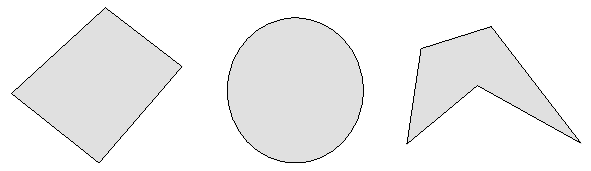
\includegraphics{chapters/chapter_2/figures/Figure5}};
		% Left pic line
		\node[circle, fill, minimum size=3pt, inner sep = 0pt] (x1) at (-4,-0.5) {};
		\node[above left] at (-4,-0.5) {$x_1$};
		\node[circle, fill, minimum size=3pt, inner sep = 0pt] (x2) at (-2.8,0.5) {};
		\node[above left] at (-2.8,0.5) {$x_2$};
		\draw[thick] (x1) -- (x2);
		% Center pic line
		\node[circle, fill, minimum size=3pt, inner sep = 0pt] (x1) at (-0.5,-0.5) {};
		\node[above left] at (-0.5,-0.5) {$x_1$};
		\node[circle, fill, minimum size=3pt, inner sep = 0pt] (x2) at (0.5,0.5) {};
		\node[above left] at (0.5,0.5) {$x_2$};
		\draw[thick] (x1) -- (x2);
		\node[circle, fill, minimum size=3pt, inner sep = 0pt] (x1) at (2.3, -0.3) {};
		\node[above] at (2.3, -0.3) {$x_1$};
		\node[circle, fill, minimum size=3pt, inner sep = 0pt] (x2) at (4,-0.3) {};
		\node[above left] at (4,-0.3) {$x_2$};
		\draw[thick] (x1) -- (x2);
	\end{tikzpicture}
	\caption{Two convex sets (left and middle) and one nonconvex set (right)} \label{p1c2:fig:convex_sets}
\end{figure}

Associated with the notion of convex sets are two important elements we will refer to later when we discuss linear problems that embed \emph{integrality requirements}. The first is the notion of a \emph{convex combination}, which is already contained in Definition \ref{p1c2:def:convex_set}, but can be generalised for an arbitrary number of points. The second consists of \emph{convex hulls}, which are sets formed by combining the convex combinations of all elements within a given set. As one might suspect, convex hulls are always convex sets, regardless of whether the original set from which the points are drawn from is convex or not. These are formalised in Definition \ref{p1c2:def:convex_combination_hull} and illustrated in Figure \ref{p1c2:fig:convex_hulls}.

\begin{definition}[Convex combinations and convex hulls] \label{p1c2:def:convex_combination_hull}
	Let $x_1, \dots, x_k \in \reals^n$ and $\lambda_1,\dots, \lambda_k \in \reals$ such that $\lambda_i \geq 0$ for $i = 1, \dots, k$ and $\sum_{i=1}^k \lambda_i = 1$. Then
	\begin{enumerate}
		\item $x = \sum_{i=1}^k \lambda_i x_i$ is a \emph{convex combination} of $\braces{x_i}_{i=1}^k \in \reals^n$;
		\item The \emph{convex hull} of $\braces{x_i}_{i=1}^k \in \reals^n$, denoted $\conv(x_1, \dots, x_k)$, is the set of all convex combinations of $\braces{x_i}_{i=1}^k \in \reals^n$.
	\end{enumerate}		
\end{definition}

\begin{figure}
	\begin{tikzpicture}
		\node (pic) at (0,0) {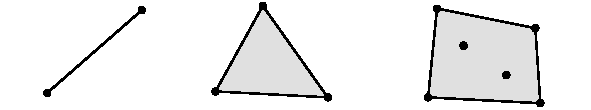
\includegraphics{chapters/chapter_2/figures/Figure6}};
		\node (x1l) at (-4.5,-0.7) {$x_1$};
		\node (x2l) at (-2.3, 0.7) {$x_2$};
		\node (x1c) at (-0.5, 1.1) {$x_1$};
		\node (x2c) at (0.8, -1) {$x_2$};
		\node (x3c) at (-1.5, -0.9) {$x_3$};
		\node (x1r) at (2.1, 1) {$x_1$};
		\node (x2r) at (4.4, 0.6) {$x_2$};
		\node (x3r) at (4.5, -0.9) {$x_3$};
		\node (x4r) at (1.9, -0.9) {$x_4$};
		\node (x5r) at (2.7, 0.4) {$x_5$};
		\node (x6r) at (3.8, -0.15) {$x_6$};
	\end{tikzpicture}
	\vspace{-6pt}
	\caption{The convex hull of two points is the line segment connecting them (left); The convex hull of three (centre) and six (right) points in $\reals^2$} \label{p1c2:fig:convex_hulls}
\end{figure}	

We are now ready to state the result that guarantees the convexity of polyhedral sets of the form
$$
	S = \braces{x \in \reals^n : Ax \le b}.
$$


\begin{theorem}[Convexity of polyhedral sets] \label{p1c2:thm:convexity}
	The following statements are true:
	\begin{enumerate}
		\item The intersection of convex sets is convex
		\item Every polyhedral set is a convex set
		\item A convex combination of a finite number of elements of a convex set also belongs to that set
		\item The convex hull of a finite number of elements is a convex set.			
	\end{enumerate}
\end{theorem}

\begin{proof}
	We provide the proof for each of the statements individually. 
	\begin{enumerate}
	 \item Let 	$S_i$, for $i \in I = \braces{1,\dots,n}$, be a collection of $n$ convex sets and suppose that $x, y \in \bigcap_{i \in I} S_i$. Let $\lambda \in [0,1]$. Since $S_i$ are convex and $x,y \in S_i$ for all $i \in I$, $\lambda x + (1-\lambda) y \in S_i$ for all $i \in I$ and, thus, $\lambda x + (1-\lambda) y \in \bigcap_{i \in I} S_i$.
	
	\item Let $a \in \reals^n$ and $b \in \reals$. Let $x,y \in \reals^n$, such that $a^\top x \geq b$ and $a^\top y \geq b$. Let $\lambda \in [0,1]$. Then $a^\top (\lambda x + (1-\lambda)y) \geq \lambda b + (1-\lambda)b = b$, showing that half-spaces are convex. The result follows from combining this with (1).    
	
	\item By induction. Let $S$ be a convex set and assume that the convex combination of $x_1, \dots, x_k \in S$ also belongs to $S$. Consider $k+1$ elements $x_1, \dots, x_{k+1} \in S$ and $\lambda_1, \dots, \lambda_{k+1}$ with $\lambda_i \in [0,1]$ for $i = 1,\dots, k+1$ and $\sum_{i=1}^{k+1}\lambda_i = 1$ and $\lambda_{k+1} \neq 1$ (without loss of generality). Then

	\begin{equation}
		\sum_{i=1}^{k+1}\lambda_i x_i = \lambda_{k+1}x_{k+1} + (1 - \lambda_{k+1}) \sum_{i=1}^k \frac{\lambda_i}{1 - \lambda_{k+1}}x_i. \label{p1c2:eq:induction}
	\end{equation}								

		Notice that $\sum_{i=1}^{k}\frac{\lambda_i}{1 - \lambda_{k+1}} = 1$. Thus, using the induction hypothesis, $\sum_{i=1}^{k}\frac{\lambda_i}{1 - \lambda_{k+1}}x_i \in S$. Considering that $S$ is convex and using \eqref{p1c2:eq:induction}, we conclude that $\sum_{i=1}^{k+1}\lambda_{k+1}x_{k+1} \in S$, completing the induction.
		
	\item Let $S = \conv(x_1, \dots, x_k)$. Let $y = \sum_{i=1}^k \alpha_i x_i$ and $z = \sum_{i=1}^k \beta_ix_i$ be such that $y,z \in S$, $\alpha_i,\beta_i \geq 0$, and $\sum_{i=1}^k \alpha_i = \sum_{i=1}^k \beta_i = 1$. Let $\lambda \in [0,1]$. Then
		%
		\begin{equation}
			\lambda y + (1- \lambda)z = \lambda\sum_{i=1}^k \alpha_i x_i + (1-\lambda)\sum_{i=1}^k \beta_i x_i = \sum_{i=1}^k (\lambda \alpha_i + (1-\lambda) \beta_i)x_i. 	
		\end{equation}
		%
		Since $\sum_{i=1}^k \lambda \alpha_i + (1-\lambda) \beta_i = 1$ and $\lambda \alpha_i + (1-\lambda) \beta_i \geq 0$ for $i=1,\dots,k$, $\lambda y + (1- \lambda)z$ is a convex combination of $x_1, \dots, x_k$ and, thus, $\lambda y + (1- \lambda)z \in S$, showing the convexity of $S$. \qedhere	
	\end{enumerate}	
\end{proof}

Figure \ref{p1c2:fig:convexity_theorem_examples} illustrates some of the statements represented in the proof. For example, the intersection of the convex sets is always a convex set. One should notice however that the same does not apply to the union of convex sets. Notice that statement 2 proves that polyhedral sets as defined according to Definition \ref{p1c2:def:polyhedral_sets} are convex. Finally the third figure on the right illustrates the convex hull of four points as a convex polyhedral set containing the lines connecting any two points within the set. 
 
\begin{figure}
	\begin{tikzpicture}
%			\draw[help lines] (-5,-1) grid (5,1);
		\node (pic) at (0,0) {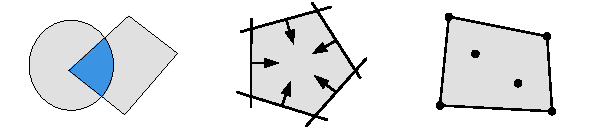
\includegraphics{chapters/chapter_2/figures/Figure7}};
	\end{tikzpicture}
    \vspace{-6pt}
	\caption{Illustration of statement 1 (left), 2 (centre), and 3 and 4 (right)} \label{p1c2:fig:convexity_theorem_examples}
\end{figure}	

We will halt our discussion about convexity for now and return to it in deeper detail in Part 2. We finish by showing a simple yet very powerful result, which states that the presence of convexity is what allows us to conclude that a locally optimal solution returned by an optimisation algorithm applied to a linear programming problem is indeed optimal for the problem at hand. It so turns out that, in the context of linear programming, convexity is a given since linear functions are convex by definition and the feasibility set of linear programming is also convex (as we have just shown in \ref{p1c2:thm:convexity}).

\begin{theorem}[Global optimality for convex problems] \label{p1c2:thm:convexity_and_optimality}
 Let $f: \reals^n \to \reals$ be a convex function, that is, $f(\lambda x_1 + (1-\lambda)x_2) \le \lambda f(x_1) + (1-\lambda)f(x_2), \ \lambda \in [0,1]$, and let $S \subset \reals^n$ be a convex set. Let $x^*$ be an element of $S$. Suppose that $x^*$ is a local optimum for the problem of minimising $f(x)$ over $S$. That is, there exists some $\epsilon > 0$ such that $f(x^*) \leq f(x)$ for all $x \in S$ for which $\|x - x^*\| \leq \epsilon$. Then, $x^*$ is globally optimal, meaning that $f(x^*) \leq f(x)$ for all $x \in S$. 
\end{theorem}

\begin{proof}
	Suppose, in order to derive a contradiction that $f(x) < f(x^*)$ for some $x \in S$. Using Definition \ref{p1c2:def:convex_set}, we have that
	$$f(\lambda x + (1-\lambda) x^*) \le \lambda f(x) + (1-\lambda) f(x^*) < \lambda f(x^*) + (1-\lambda) f(x^*) = f(x^*), \ \forall \lambda \in [0,1].$$
	
	We see that the strict inequality $f(\lambda x + (1-\lambda) x^*) < f(x^*)$ holds for any point $\lambda x + (1-\lambda) x^*$, including those with $\| \lambda x + (1-\lambda) x^* - x^* \| \le \epsilon$. Our assumption thus contradicts the local optimality of $x^*$, and this proves that $f(x) \ge f(x^*)$ for all $x \in S$.
\end{proof}




\section{Extreme points, vertices, and basic feasible solutions}

Now we focus on the algebraic representation of the most relevant geometric elements in the optimisation of linear programming problems. As we have seen in the graphical example in the previous chapter, the optimum of linear programming problems is generally located at the vertices of the feasible set. Furthermore, such vertices are formed by the intersection of $n$ constraints (in a $n$-dimensional space, which comprises constraints that are active (or satisfied at the boundary of the half-space of said constraints).

First, let us formally define the notions of vertex and extreme point. Although in general these can refer to different objects, we will see that in the case of linear programming problems, if a point is a vertex, then it is an extreme point as well, the converse also being true.

\begin{definition}[Vertex] \label{p1c2:def:vertex}
	Let $P$ be a convex polyhedral set. The vector $x \in P$ is a vertex of $P$ if there exists some $c$ such that $c^\top x < c^\top y$ for all $y \in P$ with $y \neq x$.
\end{definition}

\begin{definition}[Extreme points]\label{p1c2:def:extreme_point}
	Let $P$ be a convex polyhedral set. The vector $x \in P$ is an extreme point of $P$ if there are no two vectors $y,z \in P$ (different than $x$) such that $x = \lambda y + (1 - \lambda)z$, for any $\lambda \in [0,1]$.
\end{definition}

Figure \ref{p1c2:fig:vertex_and_extreme_point} provides an illustration of the Definitions \ref{p1c2:def:vertex} and \ref{p1c2:def:extreme_point}. Notice that the definition of a vertex involves an additional hyperplane that, once placed on a vertex point, strictly contains the whole polyhedral set in one of the half-spaces it defines, except for the vertex itself. On the other hand, the definition of an extreme point only relies on convex combinations of elements in the set itself. 

\begin{figure}
	\begin{tikzpicture}
		\node (pic) at (0,0) {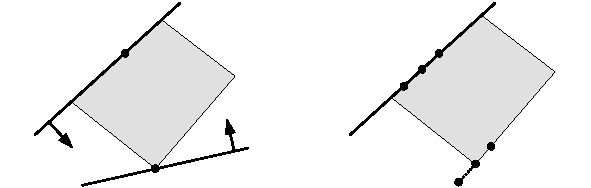
\includegraphics{chapters/chapter_2/figures/Figure8}};
		\node (Pl) at (-2.5, 0) {$P$};
		\node (Pr) at (3, 0) {$P$};
		\node (wl) at (-3, 0.9) {$w$};
		\node (xl) at (-2.3, -1.5) {$x$};
		\node (c1) at (-4, -1) {$c$};
		\node (c2) at (-0.9, -0.5) {$c$};
		\node[left] (cw) at (-2.3, 1.5) {$\braces{y : c^\top y = c^\top w}$};
		\node[right] (cx) at (-1.7, -1.4) {$\braces{y : c^\top y = c^\top x}$};
		\node (wr) at (2.1, 0.7) {$w$};
		\node (vr) at (2.4, 0.9) {$v$};
		\node (ur) at (1.8, 0.4) {$u$};
		\node (xr) at (3.1, -1.5) {$x$};
		\node (yr) at (3.4, -1.2) {$y$};
		\node (zr) at (2.8, -1.8) {$z$};
	\end{tikzpicture}
	\caption{Representation of a vertex (left) and a extreme point (right)} \label{p1c2:fig:vertex_and_extreme_point}
\end{figure}	

Definition \ref{p1c2:def:vertex} also hints an important consequence for linear programming problems. As we seen from Theorem \ref{p1c2:thm:convexity}, $P$ is convex, which guarantees that $P$ is contained in the half-space $c^\top y > c^\top x$. This  implies that $c^\top x \leq c^\top y, \forall y \in P$, which is precisely the condition that $x$ must satisfy to be the minimum for the problem $\mini_x\braces{c^\top x :x \in P}$.   

Now we focus on the description of active constraints from an algebraic standpoint. For that, let us first generalise our setting by considering all possible types of linear constraints. That is, let us consider the convex polyhedral set $P \subset \reals^n$, formed by the set of inequalities and equalities:
%
\begin{align*}
	& a_i^\top x \geq b, i \in M_1, \\ 
	& a_i^\top x \leq b, i \in M_2, \\
	& a_i^\top x = b, i \in M_3.
\end{align*}

\begin{definition}[Active (or binding) constraints] \label{p1c2:fig:active_constraint}
	If a vector $\overline{x}$ satisfies $a_i^\top \overline{x} = b_i$ for some $i \in M_1, M_2$, or $M_3$, we say that the corresponding constraints are active (or binding).
\end{definition}

Definition \ref{p1c2:fig:active_constraint} formalises the notion of active constraints. This is illustrated in Figure \ref{p1c2:fig:active_constraints}, where the polyhedral set $P = \braces{x \in \reals^3 : x_1 + x_2 + x_3 = 1, x_i \geq 0, i =1,2,3}$ is represented. Notice that, while points $A$, $B$, $C$ and $D$ have 3 active constraints, $E$ only has 2 active constraints ($x_2 = 0$ and $x_1 + x_2 + x_3 = 1$).

\begin{figure}[h]
	\begin{tikzpicture}
		\node (pic) at (0,0) {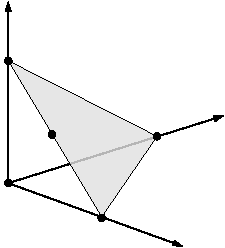
\includegraphics{chapters/chapter_2/figures/Figure9}};
		\node (x1) at (1.5, -2) {$x_1$};
		\node (x2) at (1.7, 0.4) {$x_2$};
		\node (x3) at (-2.1, 2) {$x_3$};
		\node (P) at (0, -0.5) {$P$};
		\node[left] (A) at (-1.1, 1.3) {$A$};
		\node[left] (B) at (-1.8, -1) {$B$};
		\node[right] (C) at (-0.5, -1.9) {$C$};
		\node[above] (D) at (0.9, -0.1) {$D$};
		\node[right] (E) at (-1.6, -0.2) {$E$};
	\end{tikzpicture}
	\caption{Representation of $P$ in $\reals^3$.} \label{p1c2:fig:active_constraints}
\end{figure}	

Theorem \ref{p1c2:thm:active_const} sows a thread between having a collection of active constraints forming a vertex and being able to describe it as a basis of a subspace that is formed by the vectors $a_i$ that form these constraints. This link is what will allow us to characterise vertices by their forming active constraints.

\begin{theorem}[Properties of active constraints]\label{p1c2:thm:active_const}
	Let $\overline{x} \in \reals^n$ and $I = \braces{ i \in M_1 \cup M_2 \cup M_3 : a_i^\top \overline{x} = b_i}$. Then, the following are equivalent:
	\begin{enumerate}
		\item There exists $n$ vectors in $\braces{a_i}_{i \in I}$ that are linearly independent.  
		\item The $\spans(\braces{a_i}_{i \in I})$ spans $\reals^n$. That is, every $x \in \reals^n$ can be expressed as a linear combination of $\braces{a_i}_{i \in I}$.
		\item The system of equations $\braces{a_i ^\top x = b_i}_{i \in I}$ has a unique solution.
	\end{enumerate}
\end{theorem}

\begin{proof}
	Suppose that $\braces{a_i}_{i \in I}$ spans $\reals^n$, implying that the $\spans(\braces{a_i}_{i \in I})$ has dimension $n$. By Theorem \ref{p1c2:thm:LI_and_bases} (part 1), $n$ of these vectors form a basis for $\reals^n$ and are, thus, linearly independent. Moreover, they must span $\reals^n$ and therefore every $x \in \reals^n$ can be expressed as a combination of $\braces{a_i}_{i \in I}$. This connects (1) and (2).
	
	Assume that the system of equations $\braces{a_i ^\top x = b_i}_{i \in I}$ has multiple solutions, say $x_1$ and $x_2$. Then, the nonzero vector $d = x_1 - x_2$ satisfies $a_i^\top d = 0$ for all $i \in I$. As $d$ is orthogonal to every $a_i$, $i \in I$, $d$ cannot be expressed as a combination of $\braces{a_i}_{i \in I}$ and, thus, $\braces{a_i}_{i \in I}$ do not span $\reals^n$.
	
	Conversely, if $\braces{a_i}_{i \in I}$ do not span $\reals^n$, choose $d \in \reals^n$ that is orthogonal to $\spans(\braces{a_i}_{i \in I})$. If $x$ satisfies $\braces{a_i ^\top x = b_i}_{i \in I}$, so does $\braces{a_i ^\top (x + d) = b_i}_{i \in I}$, thus yielding multiple solutions. This connects (2) and (3). \qedhere
\end{proof}

Notice that Theorem \ref{p1c2:thm:active_const} implies that there are (at least) \emph{$n$ active constraints ($a_i$)} that are \emph{linearly independent} at $\overline{x}$. This is the reason why we will refer to $\overline{x}$, and any vertex-forming solution, as a \emph{basic solution}, of which we will be interested in those that are feasible, i.e., that satisfy all constraints $i \in M_1 \cup M_2 \cup M_3$. Definition \ref{p1c2:def:basic_feasible_solution} provides a formal definition of these concepts.

\begin{definition}[Basic feasible solution (BFS)] \label{p1c2:def:basic_feasible_solution}
	Consider a convex polyhedral set $P \subset \reals^n$ defined by linear equality and inequality constraints, and let $\overline{x} \in \reals^n$.
	\begin{enumerate}
		\item $\overline{x}$ is a \emph{basic solution} if 
		\begin{enumerate}
			\item All equality constraints are active,
			\item Out of the constraints active at $\overline{x}$, $n$ of them are linearly independent, and
			\item $\overline{x}$ is the unique solution of the linear system formed by $n$ linearly-independent active constraints.
		\end{enumerate}
		\item if $\overline{x}$  is a basic solution satisfying all constraints, we say $\overline{x}$ is a basic feasible solution. 
	\end{enumerate}
\end{definition}

Figure \ref{p1c2:fig:BFS} provides an illustration of the notion of basic solutions, and show how only a subset of the basic solutions are feasible. As one might infer, these will be the points of interest in out future developments, as these are the candidates for optimal solution.

\begin{figure}[h]
	\begin{tikzpicture}
		\node (pic) at (0,0) {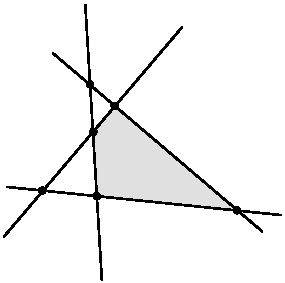
\includegraphics{chapters/chapter_2/figures/Figure10}};
		\node[above] (A) at (-0.7, 1) {$A$};
		\node[left] (B) at (-0.9, 0.2) {$B$};
		\node[right] (C) at (-0.4, 0.7) {$C$};
		\node[below] (D) at (1.6, -1.2) {$D$};
		\node[below] (E) at (-0.5, -1) {$E$};
		\node[above] (F) at (-1.8, -0.8) {$F$};
		\node (P) at (-0.3, -0.3) {$P$};
	\end{tikzpicture}
	\caption{Points $A$ to $F$ are basic solutions; $B$,$C$,$D$, and $E$ are BFS.} \label{p1c2:fig:BFS}
\end{figure}		

We finalise stating the main result of this chapter, which formally confirms the intuition we have developed so far. That is, for convex polyhedral sets, the notion of vertices and extreme points coincide, and these points can be represented as basic feasible solutions. This is precisely the link that allows for considering the feasible region of linear programming problems under a purely algebraic characterisation of the candidates for optimal solutions, those described uniquely by a subset of constraints of the problem that is assumed to be active.

\begin{theorem}[BFS, extreme points and vertices]\label{p1c2:thm:BFS_vertex_extreme_point}
	Let $P \subset \reals^n$ be a convex polyhedral set and let $\overline{x} \in P$. Then, the following are equivalent
	$$	\overline{x} \text{ is a vertex} \iff \overline{x} \text{ is an extreme point} \iff \overline{x} \text{ is a BFS}.	
	$$
\end{theorem}


\begin{proof}
	Let $P =\{ x \in \reals^n : a_i^\top x \geq b_i, i \in M_1, a_i^\top x = b_i, i \in M_2\}$, and $I = \braces{i \in M_1 \cup M_2 \mid a_i^\top x = b_i}$.
	
	\begin{enumerate}
		\item (Vertex $\Rightarrow$ Extreme point) Suppose $\overline{x}$ is a vertex. Then, there exists some $c \in \reals^n$ such that $c^\top\overline{x} < c^\top x$, for every $x \in P$ with $x \neq \overline{x}$ (cf. Definition \ref{p1c2:def:vertex}). Take $y,z \in P$ with $y,z \neq \overline{x}$. Thus $c^\top\overline{x} < c^\top y$ and $c^\top\overline{x} < c^\top z$. For $\lambda \in [0,1]$, $c^\top \overline{x} < c^\top(\lambda y + (1-\lambda)z)$ implying that $\overline{x} \neq \lambda y + (1-\lambda)z$, and is thus an extreme point (cf. Definition \ref{p1c2:def:extreme_point}).
		
		\item (Extreme point $\Rightarrow$ BFS) We will prove the contrapositive instead\footnote{Consider two propositions $A$ and $B$. Then, we have that $A \Rightarrow B \equiv \neg B \Rightarrow \neg A$. The latter is known as the \emph{contrapositive} of the former.}. Suppose $\overline{x} \in P$ is not a BFS. Then, there are no $n$ linearly independent vectors within $\braces{a_i}_{i \in I}$. Thus the vectors  $\braces{a_i}_{i \in I}$ lie in a proper subspace of $\reals^n$. Let the nonzero vector $d \in \reals^n$ be such that $a_i^\top d = 0$, for all $i \in I$.
			
			Let $\epsilon > 0$, $y = \overline{x} + \epsilon d$, and $z = \overline{x} - \epsilon d$. Notice that $a_i^\top y = a_i^\top z = b_i$, for all $i \in I$. Moreover, for $i \neq I$, $a_i^\top x > b_i$ and, provided that $\epsilon$ is sufficiently small (such that $\epsilon|a_i^\top d| < a_i ^\top \overline{x} - b_i $), we have that $a_i ^\top x \geq b_i$ for all $i \in I$. Thus $y \in P$, and by a similar argument, $z \in P$. Now, by noticing that $\overline{x} = \frac{1}{2}y + \frac{1}{2}z$, we see that $\overline{x}$ is not an extreme point. 			 
		\item (BFS $\Rightarrow$ Vertex) Let $\overline{x}$ be a BFS. Define $c = \sum_{i \in I} a_i$. Then
			\begin{equation*}
				c^\top \overline{x} = \linebreak \sum_{i \in I} a_i^\top \overline{x} = \sum_{i \in I} b_i.	 			 	
	 		\end{equation*}
			Also, for any $x \in P$, we have that 
			\begin{equation*}
				c^\top x = \sum_{i \in I} a_i^\top x \geq \sum_{i \in I} b_i, 	 	
	 		\end{equation*}
	 		since $a_i^\top x \geq b_i$ for $i \in M_1 \cup M_2$. Thus, for any $x \in P$, $c^\top \overline{x} \leq c^\top x$, making $\overline{x}$ a vertex (cf. Definition \ref{p1c2:def:vertex}). \qedhere
	\end{enumerate} 	
\end{proof}

Some interesting insights emerge from the proof of Theorem \ref{p1c2:thm:BFS_vertex_extreme_point}, upon which we will build our next developments. Once the relationship between being a vertex/extreme point and a BFS is made, it means that $\overline{x}$ can be recovered as the unique solution of a system of linear equations, these equations being the active constraints at that vertex. This means that the list of all optimal solution candidate points can be obtained by simply looking at all possible combinations of $n$ active constraints, discarding those that are infeasible. This means that the number of candidates for optimal solution is \emph{finite} and can be bounded by $\binom{m}{n}$, where $m=| M_1 \cup M_2 |$. 

\vfill
\pagebreak
\section{Exercises}

\subsection*{Exercise 2.1: Polyhedral sets \cite{bertsimas1997introduction}}
Which of the following sets are polyhedral sets?

\begin{itemize}
	\item[a)] $\{(x,y)\in\mathbb{R}^2~|~ x \cos \theta + y\sin\theta \leq 1,\theta\in[0,\pi/2],x\geq0,y\geq0\}$
	\item[b)] $\{x\in\mathbb{R}~|~ x^2-8x+15\leq 0\}$
	\item[c)] The empty set ($\emptyset$).
\end{itemize}

\subsection*{Exercise 2.2: Convexity of polyhedral sets}
Prove the following theorem.

\begin{theorem*}[Convexity of polyhedral sets] 
	%	\vspace{-3pt}
	\emph{The following convexity properties about convex sets can be said:}
	\begin{enumerate}
		\item The intersection of convex sets is convex
		\item Every polyhedral set is a convex set
		\item A convex combination of a finite number of elements of a convex set also belongs to that set
		\item The convex hull of a finite number of elements is a convex set.			
	\end{enumerate}
\end{theorem*}

Note: the proof of the theorem is proved in the notes. Use this as an opportunity to revisit the proof carefully, and try to take as many steps without consulting the text as you can. This is a great exercise to help you internalise the proof and its importance in the context of this book. I strongly advise against blindly memorising it, as I suspect you will never (in my courses, at least) be requested to recite the proof literally.


\subsection*{Exercise 2.3: Inverses, linear independence, and solving $Ax = b$} 
Prove the following theorem.

\begin{theorem*}[Inverses, linear independence, and solving $Ax = b$]
	Let $A$ be a $m \times m$ matrix. Then, the following statements are equivalent:
	\begin{enumerate}
		\item $A$ is invertible
		\item $A^\top$ is invertible
		\item The determinant of $A$ is nonzero
		\item The rows of $A$ are linearly independent
		\item The columns of $A$ are linearly independent
		\item For every $b \in \reals^m$, the linear system $Ax = b$ has a unique solution
		\item There exists some $b \in \reals^m$ such that $Ax = b$ has a unique solution.	
	\end{enumerate}	
\end{theorem*}


\subsection*{Exercise 2.4: Linear independence}
\begin{itemize}
	\item[a)] According to Theorem \ref{p1c2:thm:fundamental_linear_algebra}, if the columns (or rows) of the $m \times m$ matrix $A$ are linearly independent, the system $Ax=b$ has a unique solution for every vector $b$. Explain the significance of this result in the context of linear optimization.
	\item[b)] If the columns of $A$ are not linearly independent, the system $Ax = b$ has either no solution or infinitely many solutions. Using the notions of \emph{span} and \emph{proper subspace}, explain why this is the case. 
	\item[c)] Solve the following systems of equations. Which of these systems have an invertible coefficient matrix? 
	\begin{itemize}
		\item[] \begin{align*}
			2x_1 + 3x_2 + x_3 &= 12\\
			x_1 + 2x_2 + 3x_3 &= 12\\
			3x_1 + x_2 + 2x_3 &= 12
		\end{align*}
		\item[] \begin{align*}
			x_1 + 2x_2 + 4x_3 &= 6\\
			2x_1 + x_2 + 5x_3 &= 6\\
			x_1 + 3x_2 + 5x_3 &= 6
		\end{align*}
		\item[] \begin{align*}
			x_1 + 2x_2 + 4x_3 &= 5\\
			2x_1 + x_2 + 5x_3 &= 4\\
			x_1 + 3x_2 + 5x_3 &= 7
		\end{align*}
	\end{itemize}
\end{itemize}


\subsection*{Exercise 2.5: Properties of active constraints}
Let us consider the convex polyhedral set $P \subset \reals^n$, formed by the set of equalities and inequalities:
%
\begin{align*}
	a_i^\top x \geq b, i \in M_1, \\
	a_i^\top x \leq b, i \in M_2, \\
	a_i^\top x = b, i \in M_3.
\end{align*}
%

Prove the following result.

\begin{theorem*}[Properties of active constraints]
	Let $\overline{x} \in \reals^n$ and $I = \braces{ i \in M_1 \cup M_2 \cup M_3 \mid a_i^\top \overline{x} = b_i}$. Then, the following are equivalent:
	\begin{enumerate}
		\item There exists $n$ vectors in $\braces{a_i}_{i \in I}$ that are linearly independent.  
		\item The $\spans(\braces{a_i}_{i \in I})$ spans $\reals^n$. That is, every $x \in \reals^n$ can be expressed as a combination of $\braces{a_i}_{i \in I}$.
		\item The system of equations $\braces{a_i ^\top x = b_i}_{i \in I}$ has a unique solution.
	\end{enumerate}
\end{theorem*}

Note: see Exercise 2.2.

\subsection*{Exercise 2.6: Vertex, extreme points, and BFSs}
Prove the following result.

\begin{theorem*}[BFS, extreme points and vertices]
	Let $P \subset \reals^n$ be a convex polyhedral set and let $\overline{x} \in P$. Then, the following are equivalent
	\begin{enumerate}
		\item $\overline{x}$ is a vertex;
		\item $\overline{x}$ is a extreme point;
		\item $\overline{x}$ is a BFS;	
	\end{enumerate}
\end{theorem*}

Note: see Exercise 2.2.

\subsection*{Exercise 2.7: Binding constraints} 
Given the linear program defined by the system of inequalities below,
%
\begin{flalign*}
	\maxi & 2x_1 + x_2 && \\
	\st   & 2x_1 + 2x_2 \leq 9 && \\
		  & 2x_1 - x_2 \leq 3 && \\
		  & x_1 - x_2 \leq 1 && \\
		  & x_1 \leq 2.5 && \\
		  & x_2 \leq 4 && \\
		  & x_1, x_2 \geq 0.
\end{flalign*}
%
Assess the following points relative to the polyhedron defined in $\reals^2$ by this system and classify them as in $(i)$ belonging to which active constraint(s), and $(ii)$ being a (basic) non-feasible/feasible solution. Use Definitions \ref{p1c2:fig:active_constraint} and \ref{p1c2:def:basic_feasible_solution} to check if your classification is correct.

\begin{itemize}
	\item[a)] $(1.5,0)$
	\item[b)] $(1,0)$
	\item[c)] $(2,1)$
	\item[d)] $(1.5,3)$
\end{itemize}

 


	
	\chapter{Basis, Extreme Points and Optimality in Linear Programming} \label{chapter_3}
	\section{Polyhedral sets in standard form}

In the context of linear programming problems, we will often consider problems written in the so-called \emph{standard form}. The standard form can be understood as posing the linear programming problem as an underdetermined system of equations (that is, with fewer equations than variables). Then, we will work on selecting a subset of the variables to be set to zero so that the number of remaining variables is the same as that of equations, making the system solvable. 

A key point in this chapter will be devising how we relate this process of selecting variables with that of selecting a subset of active constraints (forming a vertex, as we have seen in the previous chapter) that will eventually lead to an optimal solution. 


\subsection{The standard form of linear programming problems}

First, let us formally define the notion of a standard-form polyhedral set. Let $A$ be a $m \times n$ matrix and $b \in \reals^m$. The \emph{standard form} polyhedral set $P$ is given by 
%
\begin{equation*}
	P = \braces{x \in \reals^n : Ax = b, ~x \geq 0}.		
\end{equation*}
%
We assume that the $m$ equality constraints are linearly independent, i.e., $A$ is full (row) rank ($m \leq n$). We know that a basic solution can be obtained from a collection of $n$ active constraints since the problem is defined in $\reals^n$. 

One important point is that \emph{any} linear programming problem can be represented in the standard form. This is achieved utilising nonnegative \emph{slack variables}. Thus, a feasibility set that is, say, originally represented as
%
\begin{equation*}
	P = \braces{x \in \reals^n : A_1 x \le b_1, A_2x \ge b_2, x \ge 0}
\end{equation*}
%
can be equivalently represented as a standard-form polyhedral set. For that, it must be modified to consider slack variables $s_1 \ge 0$ and $s_2 \geq 0$ such that
%
\begin{equation*}
	P = \braces{(x, s_1, s_2) \in \reals^{(n + |b_1| + |b_2|)} : A_1 x + s_1 = b_1, A_2x - s_2 = b_2, (x, s_1, s_2) \ge 0},
\end{equation*}
%
where $|u|$ represents the cardinality of the vector $u$. Another transformation that may be required consists of imposing the condition $x \ge 0$. Let us assume that a polyhedral set $P$ was such that (notice the absent nonnegativity condition)
%
\begin{equation*}
	P = \braces{x \in \reals^n : Ax = b}.		
\end{equation*}
%
It is a requirement for standard-form linear programs to have all variables to be assumed nonnegative. To achieve that in this case, we can simply include two auxiliary variables, say $x^+$ and $x^-$, with the same dimension as $x$, and reformulate $P$ as
 %
\begin{equation*}
	P = \braces{x^+,x^- \in \reals^n : A(x^+ - x^-) = b, x^+, x^- \ge 0}.		
\end{equation*}
%

These transformations, as we will see, will be required for employing the simplex method to solve linear programming problems with inequality constraints and, inevitably, will always render standard form linear programming problems with more variables than constraints, or $m < n$.

The standard-form polyhedral set $P$ always has, by definition, $m$ active constraints because of its equality constraints. To reach the total of $n$ active constraints, $n-m$ of the remaining constraints $x_i \ge 0$, $i =1,\dots, n$, must be made active, which can be done by selecting $n-m$ of those to be set as $x_i = 0$. These $n$ active constraints (the original $m$ plus the $n-m$ variables set to zero) form a basic solution, as we have seen in the last chapter. If it happens that the $m$ equalities can hold while the constraints $x_i \ge 0$, $i =1,\dots, n$, are satisfied, then we have a basic feasible solution (BFS). Theorem \ref{p1c3:thm:LI_and_bases} summarises this process, guaranteeing that the setting of $n-m$ variables to zero will render a basic solution.

\begin{theorem}[Linear independence and basic solutions] \label{p1c3:thm:LI_and_bases}
	Consider the constraints $Ax = b$ and $x \geq 0$, and assume that $A$ has $m$ linearly independent (LI) rows $I = \braces{1,\dots,m}$. A vector $\overline{x} \in \reals^n$ is a basic solution if and only if we have that $A \overline{x} = b$ and there exists indices $B(1), \dots, B(m)$ such that
	\begin{enumerate}
		\item[(1)] The columns $A_{B(1)}, \dots, A_{B(m)}$ of $A$ are LI
		\item[(2)] If $j \neq B(1), \dots, B(m)$, then $\overline{x}_j = 0$.
	\end{enumerate} 
\end{theorem}

\begin{proof}
	Assume that (1) and (2) are satisfied. Then the active constraints $\overline{x}_j = 0$ for $j \notin \braces{B(1), \dots, B(m)}$ and $Ax = b$ imply that
%	
	\begin{equation*}
		\sum_{i=1}^m A_{B(i)}\overline{x}_{B(i)} = \sum_{j=1}^n A_j\overline{x}_j = A\overline{x} = b.
	\end{equation*}
%
	Since the columns $\braces{A_{B(i)}}_{i \in I}$ are LI, $\braces{\overline{x}_{B(i)}}_{i \in I}$ are uniquely determined and thus $A\overline{x} = b$ has a unique solution, implying that $\overline{x}$ is a basic solution (cf. Theorem \ref{p1c2:thm:BFS_vertex_extreme_point}).
	
	Conversely, assume that $\overline{x}$ is a basic solution. Let $\overline{x}_{B(1)}, \dots, \overline{x}_{B(k)}$ be the nonzero components of $\overline{x}$. Thus, the system 
%	
		\begin{equation*}
			\sum_{i=1}^n A_i\overline{x}_i = b \text{ and } \braces{\overline{x}_i = 0}_{i \notin \braces{B(1), \dots, B(k)}}
		\end{equation*}
%
	has a unique solution, and so does $\sum_{i=1}^k A_{B(i)}\overline{x}_{B(i)} = b$, implying that the columns $A_{B(1)}, \dots, A_{B(k)}$ are LI. Otherwise, there would be scalars $\lambda_1,\dots, \lambda_k$, not all zeros, for which $\sum_{i=1}^k A_{B(i)}\lambda_i = 0$; this would imply that $\sum_{i=1}^k A_{B(i)}(\overline{x}_{B(i)} + \lambda_i) =b$, contradicting the uniqueness of $\overline{x}$.
	
	Since $A_{B(1)}, \dots, A_{B(k)}$ are LI, $k \leq m$. Also, since $A$ has $m$ LI rows, it must have $m$ LI columns spanning $\reals^m$. Using Theorem \ref{p1c2:thm:LI_and_bases}, we can obtain $m-k$ additional columns $A_{B(k+1)}, \dots, A_{B(m)}$ so that $A_{B(1)}, \dots, A_{B(m)}$ are LI. 
	
	Finally, since $k \leq m $, $\braces{\overline{x}_j = 0}_{i \notin \braces{B(1), \dots, B(m)}} \subset  \braces{\overline{x}_j = 0}_{i \notin \braces{B(1), \dots, B(k)}}$, satisfying (1) and (2). \qedhere 		
\end{proof}	

The proof of Theorem \ref{p1c3:thm:LI_and_bases} highlights an important aspect in the process of generating basic solutions. Notice that once we set $n-m$ variables to be zero, the system of equations forming $P$ becomes uniquely determined, i.e., 
%
\begin{equation*}
	\sum_{i=1}^m A_{B(i)}\overline{x}_{B(i)} = \sum_{j=1}^n A_j\overline{x}_j = A\overline{x} = b.
\end{equation*}	
%


\subsection{Forming bases for standard-form linear programming problems}

Theorem \ref{p1c3:thm:LI_and_bases} provides us with a way to develop a simple procedure to generate all basic solutions of a linear programming problem in standard form:

\begin{enumerate}
	\item Choose $m$ LI columns $A_{B(1)}, \dots, A_{B(m)}$;
	\item Let $x_j = 0$ for all $j \notin \braces{B(1), \dots, B(m)}$;
	\item Solve the system $Ax = b$ to obtain $x_{B(1)}, \dots, x_{B(m)}$.
\end{enumerate}

You might have noticed that in the proof of Theorem \ref{p1c3:thm:LI_and_bases}, the focus shifted to the columns of $A$ rather than its rows. The reason for that is because, when we think of solving the system $Ax = b$, what we are truly doing is finding a vector $x$ representing the linear combination of the columns of $A$ that yield the vector $b$. This creates an association between the columns of $A$ and the components of $x$ (i.e., the variables). Notice, however, that the columns of $A$ are not \emph{the} variables per se, as they have dimension $m$ (while $x \in \reals^n$). 

One important interpretation for Theorem \ref{p1c3:thm:LI_and_bases} is that we will form bases for the column space of $A$ by choosing $m$ components to be nonzero in a vector of dimension $n$. Since $m < n$ by definition, $A$ can only have rank $\rank(A) = \min\{m,n\} = m$, which happens to be the size of the row space of $A$ (as the rows are assumed LI). This, in turn, means that both the column and the row spaces have dimension $m$. Thus, these bases are bases for the column space of $A$. Finally, finding the vector $x$ is the same as finding how the vector $b$ can be expressed as a linear combination of that basis. Notice that this is always possible when the basis spans $\reals^m$ (as we have $m$ LI column vectors) and $b \in \reals^m$.

You will notice that from here onwards, we will implicitly refer to the columns of $A$ as variables (although we actually mean the weight associated with that column, represented by the respective component in the variable $x$). Then, when we say that we are setting some ($n-m$) of the variables to be zero, it means that we are ignoring the respective columns of $A$ (the mapping between variables and columns being their indices: $x_1$ referring to the first column, $x_2$ to the second, and so forth), while using the remainder to form a (unique) combination that yields the vector $b$, being the weights of this combination precisely the solution $x$, which in turn represent the coordinates in $\reals^n$ of the vertex formed by the $n$ ($m$ equality constraints plus $n-m$ variables set to zero) active constraints.   

As we will see, this procedure will be at the core of the simplex method. Since we will often refer to elements associated with this procedure, it will be useful to define some nomenclature.

We say that $B = \braces{A_{B(i)}}_{i \in I_B}$ is a \emph{basis} (or, perhaps more precisely, a basic matrix) with basic indices $I_B = \braces{B(1), \dots, B(m)}$. Consequently, we say that the variables $x_j$, with $j \in I_B$, are \emph{basic variables}. Somewhat analogously, we say that the variables chosen to be set to zero are the \emph{nonbasic variables} $x_j$, with $j \in I_N$, where $I_N = J \setminus I_B$, with $J = \braces{1, \dots, n}$ being the indices of all variables (and all columns of $A$).
 
 Notice that the basic matrix $B$ is invertible since its columns are LI (c.f. Theorem \ref{p1c2:thm:LI_and_bases}). For $x_B = (x_{B(1)}, \dots, x_{B(m)})$, the \emph{unique solution} for $Bx_B = b$ is 
%
\begin{equation*}
	x_B = B^{-1}b, \text{ where } 
	B = \begin{bmatrix} \vline & \vline & \vline \\
					  A_{B(1)} & \dots & A_{B(m)} \\
	    	    		\vline & \vline & \vline	
		\end{bmatrix} \text{ and } 
	x_B =  \begin{bmatrix}   x_{B(1)} \\
		 			     		 \vdots   \\
		 			     		 x_{B(m)}	
		   \end{bmatrix}.
\end{equation*}
%

Let us consider the following numerical example. Consider the following set $P$
%
\begin{equation}  \label{p1c3:eq:example_P}
	P = \left\{x \in \reals^3 :  
		\begin{aligned}
			& x_1 + x_2 + 2x_3 \le 8 \\
			& x_2 + 6 x_3 \le 12 \\
			& x_1 \le 4 \\
			& x_2 \le 6 \\
			& x_1, x_2, x_3 \ge 0
		\end{aligned}
		\right\}, 	
\end{equation}
%
which can be written in the standard by adding slack variables $\braces{x_i}_{i \in \{4,\dots,7\}}$, yielding 
%
\begin{equation}  \label{p1c3:eq:example_P}
	P = \left\{x \in \reals^7 :  
		\begin{aligned}
			& x_1 + x_2 + 2x_3 + x_4 = 8 \\
			& x_2 + 6 x_3 + x_5 = 12 \\
			& x_1 + x_6 = 4 \\
			& x_2 + x_7 =6 \\
			& x_1, \dots, x_7 \ge 0
		\end{aligned}
		\right\}. 	
\end{equation}
%
The system $Ax=b$ can be represented as 
%  
\begin{equation*}
	\begin{bmatrix}
		1 & 1 & 2 & 1 & 0 & 0 & 0 \\
		0 & 1 & 6 & 0 & 1 & 0 & 0 \\
		1 & 0 & 0 & 0 & 0 & 1 & 0 \\
		0 & 1 & 0 & 0 & 0 & 0 & 1
	\end{bmatrix} x =
	\begin{bmatrix}
		8  \\
		12 \\
		4  \\
		6   	
	\end{bmatrix}.
\end{equation*}
%
Following our notation, we have that $m = 4$ and $n = 7$. The rows of $A$ are LI, meaning that $\rank(A) = 4$\footnote{You can see for yourself using Gaussian elimination or row reduction. Tip: do the elimination on the transpose $A^\top$ instead, recalling that $\rank(A) = \rank(A^\top)$.}. We can make arbitrary selections of $n-m = 3$ variables to be set to zero (i.e., nonbasic) and calculate the value of the remaining (basic) variables. For example:
\begin{itemize}
	\item Let $I_B = \braces{4, 5, 6, 7}$; in that case $x_B = (8,12,4,6)$ and $x = (0,0,0,8,12,4,6)$, which is a basic feasible solution (BFS), as $x \geq 0$.
	\item For $I_B = \braces{3,5,6,7}$, $x_B = (4,-12,4,6)$ and $x = (0, 0, 4, 0, -12, 4, 6)$, which is basic but not feasible, since $x_5 < 0$.	
\end{itemize}


\subsection{Adjacent basic solutions}

Now that we know how a solution can be recovered, the next important concept that we need to define is how we, from one basic solution, move to an \emph{adjacent} solution. This will be the mechanism that the simplex method will utilise to move from one solution to the next in the search for the optimal solution.

Let us start formally defining the notion of an adjacent basic solution.
%
\begin{definition}[Adjacent basic solutions]
	Two basic solutions are adjacent if they share $n-1$ LI active constraints. Alternatively, two bases $B_1$ and $B_2$ are adjacent if all but one of their columns are the same.
\end{definition}
%
For example, consider the set polyhedral set $P$ defined in \eqref{p1c3:eq:example_P}. Our first BFS was defined by making $x_1 = x_2 = x_3 = 0$ (nonbasic index set $I_N = \braces{1,2,3}$). Thus, our basis was $I_B = \braces{4,5,6,7}$. An adjacent basis was then formed, by replacing the basic variable $x_4$ with the nonbasic variable $x_3$, rendering the new (not feasible) basis $I_B = \braces{3,5,6,7}$.

Notice that the process of moving between adjacent bases has a simple geometrical interpretation. Since adjacent bases share all but one basic element, this means that the two must be connected by a line segment (in the case of the example, it would be the segment between $(0,8)$ and $(4,0)$, projected onto $(x_3,x_4) \in \reals^2$, or equivalently, the line between $(0,0,0,8,12,4,6)$ and $(0,0,4,0,-12,4,6)$ (Notice how the coordinate $x_6$ also changed values; this is necessary, so the movement is made along the edge of the polyhedral set. This will become clearer when we analyse the simplex method in further detail in Chapter \ref{chapter_4}. 



\subsection{Redundancy and degeneracy}

An important underlying assumption in Theorem \ref{p1c3:thm:LI_and_bases} is that the matrix $A$ in the definition of the polyhedral set $P$ is full (row) rank, that is, there are $m$ linearly independent rows and thus $m$ independent columns. Theorem \ref{p1c3:thm:red_const} shows that this assumption can actually be made without loss of generality. 
 
\begin{theorem}[Redundant constraints]\label{p1c3:thm:red_const}
	Let $P = \braces{x \in \reals^n : Ax = b, x \geq 0}$, where $A$ is $m \times n$ matrix with rows $\braces{a_i}_{i \in I}$ and $I = \braces{1,\dots,m}$. Suppose that $\rank(A) = k < m$ and that the rows $a_{i_1}, \dots, a_{i_k}$ are LI. Then $P$ is the same set as $Q = \braces{ x \in \reals^n : a^\top_{i_1}x = b_{i_1}, \dots, a^\top_{i_k}x = b_{i_k}, x \geq 0}$.
\end{theorem}

\begin{proof}
	Assume, without loss of generality, that $i_1 = 1$ and $i_k = k$. Clearly, $P \subset Q$, since a solution satisfying the constraints forming $P$ also satisfies those forming $Q$.
	
	As $\rank(A) = k$, the rows $a_{i_1}, \dots, a_{i_k}$ form a basis in the row space of $A$ and any row $a_i$, $i \in I$, can be expressed as $a^\top_i = \sum_{j=1}^k \lambda_{ij}a_j^\top$ for $\lambda_{ij} \in \reals$.
	
	For $y \in Q$ and $i \in I$, we have $a_i^\top y = \sum_{j=1}^k \lambda_{ij}a_j^\top y = \sum_{j=1}^k \lambda_{ij}b_{j} = b_i$, which implies that $y \in P$ and that $Q \subset P$. Consequently, $P = Q$. \qedhere			
\end{proof}

Theorem \ref{p1c3:thm:red_const} implies that any linear programming problem in standard form can be reduced to an equivalent problem with linearly independent constraints. It turns out that, in practice, most professional-grade solvers (i.e., software that implements solution methods and can be used to find optimal solutions to mathematical programming models) have \emph{preprocessing} routines to remove redundant constraints. This means that the problem is automatically treated to become smaller by not incorporating unnecessary constraints. 

Degeneracy is somewhat related to the notion of redundant constraints. We say that a given vertex is a \emph{degenerate} basic solution if it is formed by the intersection of more than $n$ active constraints (in $\reals^n$). Effectively, this means that more than $n-m$ variables (i.e., some of the basic variables) are set to zero, which is the main way to identify a degenerate BFS. Figure \ref{p1c3:fig:figure1} illustrates a case in which degeneracy is present.

\begin{figure}[h]
	\begin{tikzpicture}
		\node (picture) at (0,0) {\includegraphics{chapters/chapter_3/figures/figure1.pdf}};
		\node (A) at (-4.35,-0.6) {$A$};
		\node (B) at (-1.3,-0.9) {$B$};
		\node (C) at (2.2, 1.7) {$C$};
		\node (D) at (0.2, -0.5) {$D$};		
	\end{tikzpicture}
	\caption{$A$ is a degenerate basic solution, $B$ and $C$ are degenerate BFS, and $D$ is a BFS.} \label{p1c3:fig:figure1}
\end{figure} 

Notice that, while in the figure on the left, the constraint causing degeneracy is redundant, that is not the case in the figure on the righthand side. That is, redundant constraints may cause degeneracy, but not all constraints causing degeneracy are redundant.

As another example, in some cases, we may see that degeneracy is caused by the chosen representation of the problem. For example, consider the two equivalent sets:
%
\begin{equation*}
	P_1 = \braces{(x_1, x_2,x_3) : x_1 - x_2 = 0, x_1 + x_2 + 2x_3 = 2, x_1, x_3 \geq 0} \text { and } P_2 = P_1 \cap \braces{x_2 \geq 0}. 
\end{equation*}	
%
The polyhedral set $P_2$ is equivalent to $P_1$ since $x_2 \ge 0$ is a redundant constraint. In that case, one can see that, while the point $(0,0,1)$ is not degenerate in $P_1$, it is in $P_2$, which illustrates the weak but existent relationship between redundancy and degeneracy. This is illustrated in Figure \ref{p1c3:fig:redundancy_and_degeneration}.
%
\begin{figure}[h]
	\begin{tikzpicture}
		\node (pic) at (0,0) {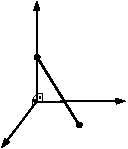
\includegraphics{chapters/chapter_3/figures/Figure2.pdf}};
		\node[right] (1) at (-0.4, 0.4) {$(0,0,1)$};
		\node[right] (2) at (0.4, -0.8) {$(1,1,0)$};	
	\end{tikzpicture}
    \caption{$(0,0,1)$ is degenerate if you add the constraint $x_2 \ge 0$.} \label{p1c3:fig:redundancy_and_degeneration}
\end{figure}

In practice, degeneracy might cause issues related to the way we identify vertices. Because more than $n$ active constraints form the vertex, and yet, we identify vertices by groups of $n$ constraints to be active, it means that we might have a collection of adjacent bases that, in fact, are representing the same (vertex) point in space, meaning that we might be ``stuck'' for a while in the same position while scanning through adjacent bases. The numerical example below illustrates this phenomenon. 

Let us consider again the example in \eqref{p1c3:eq:example_P}. 
%
\begin{equation*}
	\begin{bmatrix}
		1 & 1 & 2 & 1 & 0 & 0 & 0 \\
		0 & 1 & 6 & 0 & 1 & 0 & 0 \\
		1 & 0 & 0 & 0 & 0 & 1 & 0 \\
		0 & 1 & 0 & 0 & 0 & 0 & 1
	\end{bmatrix} 
	x =
	\begin{bmatrix}
		8  \\
		12 \\
		4  \\
		6   	
	\end{bmatrix}
\end{equation*}
%
Observe the following, 
%
\begin{itemize}
	\item let $I_B = \braces{1,2,3,7}$; this implies that $x = (4,0,2,0,0,0,6)$. There are 4 zeros (instead of $n-m=3$) in $x$, which indicates degeneracy. 
	\item Now, let = $I_B = \braces{1,3,4,7}$. This also implies that $x = (4,0,2,0,0,0,6)$. The two bases are adjacent yet represent the same point in $\reals^7$.	
\end{itemize}
%
As we will see, there are mechanisms that prevent the simplex method from becoming stuck on such vertices forever, an issue that is referred to as \emph{cycling}. 



\section{Optimality of extreme points}

Now that we have discussed how to algebraically represent extreme points and have seen a simple mechanism to iterate among their adjacent neighbours, the final element missing for us to be able to devise an optimisation method is to define the optimality conditions we wish to satisfy. In other words, we must define the conditions that, once satisfied, mean that we can stop the algorithm and declare the current solution optimal.


\subsection{The existence of extreme points}

First, let us define the condition that guarantees the existence of extreme points in a polyhedral set. Otherwise, there is no hope of finding an optimal solution.

\begin{definition}[Existence of extreme points]\label{p1c3:def:line_containing}
	A polyhedral set $P \subset \reals^n$ contains a line if $P \neq \emptyset$ and there exists a nonzero vector $d \in \reals^n$ such that $x + \lambda d \in P$ for all $\lambda \in \reals$.
\end{definition}

Figure \ref{p1c3:fig:line_containing} illustrates the notion of containing a line and the existence of extreme points. Notice that if a set would have any ``corner'', then that would imply that the edges that form that corner prevent a direction (or a line) to be fully contained within the set. Furthermore, the said corner would be an extreme point.

\begin{figure}[h]
	\begin{tikzpicture}
		\node at (0,0) {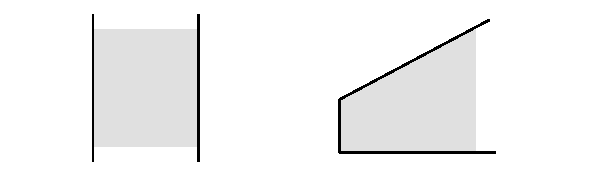
\includegraphics{chapters/chapter_3/figures/Figure3.pdf}};
		\node at (-2.5,0) {$P$};
		\node at (2,-0.3) {$Q$};		
	\end{tikzpicture}
	\caption{$P$ contains a line (left) and $Q$ does not contain a line (right)} \label{p1c3:fig:line_containing}	
\end{figure}

We are now ready to pose the result that utilises Definition \ref{p1c3:def:line_containing} to provide the conditions for the existence of extreme points.

\begin{theorem}[Existence of extreme points]\label{p1c3:thm:exist_extreme_point}
	Let $P = \braces{x \in \reals^n : a_i^\top x \geq b_i, i = 1, \dots, m} \neq \emptyset$ be a polyhedral set. Then the following are equivalent:
	\begin{enumerate}
		\item[(1)] $P$ has at least one extreme point;
		\item[(2)] $P$ does not contain a line;
		\item[(3)] There exists $n$ LI vectors within $\braces{a_i}_{i=1}^m$.	
	\end{enumerate}	
\end{theorem}	 

\begin{proof}
We start with $(2) \Rightarrow (1)$, i.e., if $P$ does not contain a line, then it must have a basic feasible solution and thus, cf. Theorem \ref{p1c2:thm:BFS_vertex_extreme_point}, an extreme point. Let $x \in \reals^n$ be an element of $P$ and let $I = \braces{i : a_i^\top x = b_is}$. If $n$ of the vectors $a_i$, $i \in I$, are linearly independent, then $x$ is a basic feasible solution, cf. Definition \ref{p1c2:def:basic_feasible_solution}. 

If less than $n$ vectors are linearly independent, then all vectors $a_i$, $i \in I$, lie in a proper subspace of $\reals^n$ and, consequently, there exists a nonzero vector $d \in \reals^n$ such that $a_i^\top d = 0$ for every $i \in I$. Consider the line consisting of all points of the form $y = x + \lambda d$, with $\lambda \in \reals$. For $i \in I$, we have that 
	$$
	a_i^\top y = a_i^\top x + \lambda a_i^\top d = a_i^\top x = b.
	$$
	Thus, the active constraints remain active at all points on the line. Now, by assumption, the polyhedral set contains no lines, and thus there will be values for $\lambda$ for which some constraint will eventually be violated. Let $\overline{\lambda}$ be the point at which this new constraint $j \not\in I$ becomes active, i.e., $a_j^\top x + \overline{\lambda}= b_j$.
	
	We must show that $a_j$ is not a linear combination of $\braces{a_i}_{i \in I}$. We know that $a_j^\top x \neq b_j$, as $j \not\in I$ and that $a_j^\top x + \overline{\lambda}= b_j$ by the definition of $\overline{\lambda}$. This implies that $a_j^\top d \neq 0$. Contrasting this with the fact that $a_i^\top d = 0$, $\forall i \in I$, we conclude that $a_j$ is linearly independent of $\braces{a_i}_{i \in I}$\footnote{To see that, notice that $d$ is orthogonal to any linear combination of vectors $\braces{a_i}_{i \in I}$ whilst it is not orthogonal to $a_j$ and, thus, $a_j$ cannot be expressed as a linear combination of $\braces{a_i}_{i \in I}$.}. 
	
	To conclude, we can see that by moving from $x$ to $x + \overline{\lambda}d$, the number of linearly independent active constraints is increased by one. Repeating the see procedure as many times as needed, we will eventually reach a point having $n$ linearly independent constraints, being thus a basic feasible solution, as we retain feasibility in the process.
	
	To show that $(1) \Rightarrow (3)$, we simply need to notice that if $P$ has an extreme point $x$, then it is also a basic feasible solution (cf. Theorem \ref{p1c2:thm:BFS_vertex_extreme_point}) and there are $n$ active constraints corresponding to $\braces{a_i}_{i \in I}$ linearly independent vectors.

	Finally, let us show that $(3) \Rightarrow (2)$ by contradiction. Assume, without loss of generality, that $a_1, \dots, a_n$ are the $n$ linearly independent vectors. Suppose that $P$ contains a line $x + \lambda d$ where $d \neq 0$. Therefore, we have that $a_i^\top x \ge b_i$, for all $i = 1, \dots, m$ and for any $\lambda$. The only way this is possible is if $a_i^\top d =0$ for all $i = 1, \dots, m$, which implies that $d=0$, reaching a contradiction that establishes that $P$ does not contain a line.
\end{proof}


It turns out that linear programming problems in the standard form do not contain a line, meaning that they will always provide at least one extreme point (and, consequently, a basic feasible solution, cf. Theorem \ref{p1c2:thm:BFS_vertex_extreme_point}). More generally, bounded polyhedral sets do not contain a line, and neither does the positive orthant.

We are now to state the result that proves the intuition we had when analysing the plots in Chapter \ref{chapter_1}, which states that if a polyhedral set has at least one extreme point and at least one optimal solution, then there must be an optimal solution that is an extreme point.

\begin{theorem}[Optimality of extreme points]\label{p1c3:thm:opt_extreme}
		Let $P = \braces{x \in \reals^n : Ax \geq b}$ be a polyhedral set and $c \in \reals^n$. Consider the problem 
			\begin{equation*}
		    		z = \mini\braces{c^\top x : x \in P}.					
			\end{equation*}
		Suppose that $P$ has at least one extreme point and that there exists an optimal solution. Then, there exists an optimal solution that is an extreme point of $P$.
\end{theorem}

\begin{proof}
	Let $Q = \braces{x \in \reals^n : Ax \geq b, c^\top x = z}$ be the (nonempty) polyhedral set of all optimal solutions. Since $Q \subset P$ and $P$ contains no line (cf. Theorem \ref{p1c3:thm:exist_extreme_point}), $Q$ contains no line either, and thus has an extreme point.

	Let $\overline{x}$ be an extreme point of $Q$. By contradiction, assume that $\overline{x}$ is not an extreme point of $P$. Then, there exist $y \neq \overline{x}$, $w \neq \overline{x}$, and $\lambda \in [0,1]$ such that $\overline{x} = \lambda y + (1-\lambda)w$. Then, $c^\top \overline{x} = \lambda (c^\top y) + (1-\lambda)c^\top w$. As $c^\top \overline{x} = z$ is optimal, we have that $z \leq c^\top y$ and $z \leq c^\top w$,  and thus $z = c^\top y = c^\top w$. 
	
	Thus, $w \in Q$ and $y \in Q$, which contradicts that $\overline{x}$ is an extreme point. Thus, $\overline{x}$ must be an extreme point and, since we established that $\overline{x} \in Q$, it is also optimal. 
\end{proof}

Theorem \ref{p1c3:thm:opt_extreme} is posed in a somewhat general way, which might be a source for confusion. First, recall that in the example in Chapter \ref{chapter_1}, we considered the possibility of the objective function level curve associated with the optimal value to be parallel to one of the edges of the feasible region, meaning that instead of a single optimal solution (a vertex), we would observe a line segment containing an infinite number of optimal solutions, of which exactly two would be extreme points. 

This is important because we intend to design an algorithm that only inspects extreme points. This discussion guarantees that, even for the cases in which a whole set of optimal solutions exists, some elements in that set will be extreme points anyway and thus identifiable by our method.

In a more general case (with $n > 2$) it might be so that a whole facet of optimal solutions is obtained. That is precisely the polyhedral set of all optimal solutions $Q$ in the proof. This polyhedral set will not contain a line and, therefore (cf. Theorem \ref{p1c3:thm:exist_extreme_point}), have at least one extreme point. 

Perhaps another important point is to notice that the result is posed assuming a minimisation problem, but it naturally holds for maximisation problems as well. Maximising a function $f(x)$ is the same as minimising $-f(x)$, with the caveat that, although the optimal value $x^*$ is the same in both cases, the optimal values are symmetric in sign (because of the additional minus we included in the problem being originally maximised).


\subsection{Finding optimal solutions}

We now focus on the issue of being able to find and recognise extreme points as optimal solutions. In general, optimisation methods iterate the following steps:
%
\begin{enumerate}
	\item Start from an initial (often feasible) solution;
	\item Find a nearby solution with better value;
	\item If none are available, return the best-known solution.	
\end{enumerate}
%
This very simple procedure happens to be the core idea of most optimisation methods. We will concentrate on how to identify directions of improvement and, as a consequence of their absence, how to identify optimality.

Starting from a point $x \in P$, we would like to move in a direction $d$ that yields improvement while maintaining feasibility. Definition \ref{p1c3:def:feasible_direction} provides a formalisation of this idea.

\begin{definition}[Feasible directions] \label{p1c3:def:feasible_direction}
	Let $x \in P$, where $P \subset \reals^n$ is a polyhedral set. A vector $d \in \reals^n$ is a feasible direction at $x$ if there exists $\theta > 0$ for which $x + \theta d \in P$.
\end{definition}

Figure \ref{p1c3:fig:feasible_directions} illustrates the concept. Notice that at extreme points, the relevant feasible directions are those along the edges of the polyhedral set since those are the directions that can lead to other extreme points.
  
\begin{figure}[h]
	\begin{tikzpicture}
		\node (0,0) {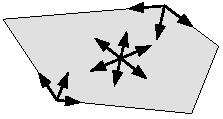
\includegraphics{chapters/chapter_3/figures/Figure4.pdf}};
		\node (P) at (-0.9,0.25) {$P$};
	\end{tikzpicture}
	\caption{Feasible directions at different points of $P$} \label{p1c3:fig:feasible_directions}
\end{figure}

Let us now devise a way of identifying feasible directions algebraically. For that, let $A$ be a $m \times n$ matrix, $I = [m]$ and $J = [n]$. Consider the problem 
%
\begin{equation*}
	\mini \braces{c^\top x : Ax = b, x \geq 0}.	
\end{equation*}
%
Let $x$ be a basic feasible solution (BFS) with basis $B = [A_{B(1)}, \dots, A_{B(m)}]$. Recall that the basic variables $x_B$ are given by
%
\begin{equation*}
	x_B = (x_{B(i)})_{i \in I_B} = B^{-1}b, \text{ with } I_B = \braces{B(1), \dots, B(m)} \subset J,	
\end{equation*}
%
and that the remaining nonbasic variables $x_N$ are such that $x_N = (x_j)_{j \in I_N} = 0$, with $I_N = J \setminus I_B$.

Moving to a neighbouring solution can be achieved by simply moving between adjacent bases, which can be accomplished without a significant computational burden. This entails selecting a nonbasic variable $x_j$, with $j \in I_N$, and increasing it to a positive value $\theta$. 

Equivalently, we can define a \emph{feasible direction} $d = [d_N, d_B]$, where $d_N$ represent the components associated with nonbasic variables and $d_B$ those associated with basic variables and move from the point $x$ to the point $x + \theta d$. The components $d_N$ associated with the nonbasic variables are thus defined as 
%
\begin{equation*}
d = \begin{cases} d_j = 1 \\ 
				  d_{j'} = 0, \text{for all } j' \neq j, 
	\end{cases}	
\end{equation*}
%
with $j, j' \in I_N$. Notice that, geometrically, we are moving along a line in the dimension represented by the nonbasic variable $x_j$.

Now, feasibility might become an issue if we are not careful to retain feasibility conditions. To retain feasibility, we must observe that $A(x + \theta d) = b$, implying that $Ad = 0$. This allows us to define the components $d_B$ of the direction vector $d$ that is associated with the basic variables $x_j$, with $j \in I_B$, since
%
\begin{equation*}
	0 = Ad = \sum_{j = 1}^n	A_j d_j = \sum_{i = 1}^m A_{B(i)}d_{B(i)} + A_j = Bd_B + A_j
\end{equation*}
%
and thus $d_B = -B^{-1} A_j$ is the \emph{basic direction} implied by the choice of the nonbasic variable $x_j$, $j \in I_N$, to become basic. The vector $d_B$ can be thought of as the adjustments that must be made in the value of the other basic variables to accommodate the new variable becoming basic to retain feasibility. 

% TODO: Chp3: this is a complicated concept using a complicated figure.  Rethink this showing a simple example (x_1 + x_2 + x_3 = 1, x_j >= 0) with the "normal feasible region" and the schematic 2d representation. by its side, showing that making 2 out of 3 variables nonbasic yields each of the corners of the triangle. 

Figure \ref{p1c3:fig:adjacent_vertices} provides a schematic representation of this process, showing how the change between adjacent basis can be seen as a movement between adjacent extreme points. Notice that it conveys a schematic representation of a $n=5$ dimensional problem, in which we ignore all the $m$ dimensions and concentrate on the $n-m$ dimensional projection of the feasibility set. This implies that the only constraints left are those associated with the nonnegativity of the variables $x \ge 0$, each associated with an edge of this alternative representation. Thus, when we set $n-m$ (nonbasic variables) to zero, we identify an associated extreme point. As $n-m = 2$, we can plot this alternative representation on $\reals^2$.

\begin{figure}[h]
	\begin{tikzpicture}
		\node (0,0) {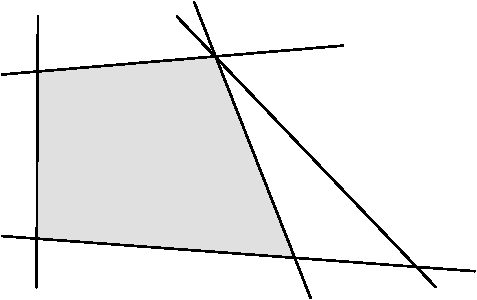
\includegraphics{chapters/chapter_3/figures/Figure5.pdf}};
		\node (A) at (-3.2, 1.65) {$A$};
		\node (B) at (-0.2, 1.9) {$B$};
		\node (C) at (3.1, -1.7) {$C$};
		\node[rotate = 90] (x1) at (-3.65, 0) {$x_1 = 0$};
		\node (x2) at (-1.2, -2) {$x_2 = 0$};
		\node (x3) at (-1.9, 1.75) {$x_3 = 0$};
		\node[left] (x4) at (0.25, 0) {$x_4 = 0$};
		\node[right] (x4) at (1.25, 0) {$x_5 = 0$};
	\end{tikzpicture}
	\caption{Example: $n = 5$ and $n-m = 2$. At $A$, $x_1 = x_3 = 0$ and $x_2, x_4, x_5 \geq 0$. Increasing $x_1$ while keeping $x_3$ zero leads to $B$. At $B$, suppose $I_N = \braces{3,5}$; by increasing $x_3$ while keeping $x_5$ zero would leads to $C$.} \label{p1c3:fig:adjacent_vertices}
\end{figure}

Overall feasibility, i.e., ensuring that $x \ge 0$, can only be retained if $\theta > 0$ is chosen appropriately small. This can be achieved if the following is observed:
%
\begin{enumerate}
	\item All the other nonbasic variables remain valued at zero, that is, $x_{j'} = 0$ for $j' \in I_N \setminus \braces{j}$.	
	\item If $x$ is a \emph{nondegenerate} extreme point, then all $x_B > 0$ and thus $x_B + \theta d_B \geq 0$ for appropriately small $\theta > 0$. 
	\item If $x$ is a \emph{degenerate} extreme point: $d_{B(i)}$ might not be feasible since, for some $B(i)$, if $d_{B(i)} < 0$ and $x_{B(i)} = 0$, any $\theta > 0$ will make $x_{B(i)} < 0$.
\end{enumerate}
%
We will see later that we can devise a simply rule to define a value for $\theta$ that guarantees the above will be always observed. For now, we will put this discussion on hold and focus on the issue of how to guide the choice of which nonbasic variable $x_j$, $j \in I_N$, to select to become basic.


\subsection{Moving towards improved solutions}

A simple yet efficient way of deciding which nonbasic component $j \in I_N$ to make basic is to consider the immediate potential benefit that it would have for the objective function value. 

Using objective function $c^\top x$, if we move along the feasible direction $d$ as previously defined, we have that the objective function value changes by 
%
\begin{equation*}
	c^\top d = c_B^\top d_B + c_j = c_j - c_B^\top B^{-1}A_j,
\end{equation*}
%
where $c_B = [c_{B(1)}, \dots, c_{B(m)}]$. The quantity $c_j - c_BB^{-1}A_j$ can be used, for example, in a greedy fashion, meaning that we choose the nonbasic variable index $j \in I_N$ with greatest \emph{potential of improvement}.

First, let us formally define this quantity, which is known as the \emph{reduced cost}. 

\begin{definition}[Reduced cost]
	Let $x$ be a basic solution associated with the basis $B$ and let $c_B = [c_{B(1)}, \dots, c_{B(m)}]$ be the objective function coefficients associated with the basis $B$. For each nonbasic variable $x_j$, with $j \in I_N$, we define the reduced cost $\overline{c}_j$ as
	%
	\begin{equation*}
		\overline{c}_j = c_j - c_B^\top B^{-1}A_j.
	\end{equation*}
\end{definition}

The name reduced cost refers to the fact that it quantifies a cost change onto the reduced space of the basic variables. In fact, the reduced cost is calculating the change in the objective function caused by the increase in one unit of the nonbasic variable $x_j$ elected to become basic (represented by the $c_j$ component) and the associated change caused by the accommodation in the basic variable values to retain feasibility ($-c_B^\top B^{-1}A_j$). Therefore, the reduced cost can be understood as a \emph{marginal value} of change in the objective function value associated with each nonbasic variable.

Let us demonstrate this with a numerical example. Consider the following linear programming problem
%
\begin{align*}
	\mini & 2x_1 + 1x_2 + 3x_3 + 2x_4 \\	
	\st & x_1 + x_2 + x_3 + x_4 = 2 \\
	& 2x_1 + 3x_3 + 4x_4 = 2 \\
	& x_1, x_2 ,x_3, x_4 \geq 0.  
\end{align*}  
%
Let $I_B = \braces{1,2}$, yielding
% 
\begin{equation*}
	B = \begin{bmatrix}
    		1 & 1 \\
    		2 & 0
    	\end{bmatrix}.
\end{equation*} 
%
Thus, $x_3= x_4 =0$ and $x = (1,1,0,0)$. The basic direction $d_B^3$ for $x_3$ is given by
%
\begin{equation*}
    d_B^3 = -B^{-1}A_3 = -\begin{bmatrix}
    	0 & 1/2 \\
    	1 & -1/2
    \end{bmatrix} \begin{bmatrix}
    	1 \\ 3
    \end{bmatrix} = \begin{bmatrix}
    	-3/2 \\ 1/2
    \end{bmatrix}.
\end{equation*}
%
which gives $d^3 = (-3/2, 1/2, 1, 0)$. Analogously, for $x_4$, we have
%
\begin{equation*}
    d_B^4 = -B^{-1}A_4 = -\begin{bmatrix}
    	0 & 1/2 \\
    	1 & -1/2
    \end{bmatrix} \begin{bmatrix}
    	1 \\ 4
    \end{bmatrix} = \begin{bmatrix}
    	-2 \\ 1
    \end{bmatrix}.
\end{equation*}

The (reduced) cost of moving along the direction given by $d^3$ is 
%
\begin{equation*}
	c^\top d^3 = (c_1, c_2)^\top d_B^3 + c_3 = ((-3/2)2 + (1/2)1) + 3 = 0.5
\end{equation*}
%
while moving along $d^4$ has a cost of
\begin{equation*}
	c^\top d^4 = (c_1, c_2)^\top d_B^4 + c_4 = ((-2)2 + (1)1) + 2 = -1.
\end{equation*}
%
Thus, between $d^3$ and $d^4$, $d^4$ is a better direction since its reduced cost indicates a reduction of $1$ unit of the objective function per unit of $x_4$. In contrast, the reduced cost associated with $d^3$ indicates an increase of 0.5 units of the objective function per unit of $x_3$, indicating that this is a direction to be avoided as we are minimising the problem.
%
Clearly, the willingness to choose $x_{j'}$, with $j' \in I_N$, as the variable to become basic will depend on whether the scalar $c_{j'} - (c_j)_{j \in I_B}^\top d_B$ is negative (recall that we want to minimise the problem, so the smaller the total cost, the better). Another point is how large in module the reduced cost is. Recall that the reduced cost is, in fact, a measure of the marginal value associated with the increase in value of the nonbasic variable. Thus, the more negative it is, the quicker the objective function value will decrease per unit of increase of the nonbasic variable value.
%
One interesting thing to notice is the reduced cost associated with basic variables. Recall that $B = [A_{B(1)}, \dots, A_{B(m)}]$ and thus $B^{-1}[A_{B(1)}, \dots, A_{B(m)}] = I$. Therefore $B^{-1}A_{B(i)}$ is the $i^\text{th}$ column of $I$, denoted $e_i$, implying that
%
\begin{equation*}
	\overline{c}_{B(i)} = c_{B(i)} - c^\top_B B^{-1} A_{B(i)} = c_{B(i)} - c_B^\top e_i = c_{B(i)} - c_{B(i)} = 0.	
\end{equation*}


\subsection{Optimality conditions}

Now that we have seen how to identify promising directions for improvement, we have incidentally developed a framework for identifying the optimality of a given basic feasible solution (BFS). That is, a BFS from which no direction of improvement can be found must be locally optimal. And, since local optimality implies global optimality in the presence of convexity (cf. Theorems \ref{p1c2:thm:convexity} and \ref{p1c2:thm:convexity_and_optimality}), we can declare this BFS as an optimal solution. 

Theorem \ref{p1c3:thm:opt_conditions} establishes the optimality of a BFS from which no improving feasible direction can be found without explicitly relying on the notion of convexity.

\begin{theorem}[Optimality conditions]\label{p1c3:thm:opt_conditions}
	Consider the problem $P : \mini\braces{c^\top x : Ax = b, x \geq 0}$. Let $x$ be the BFS associated with a basis $B$ and let $\overline{c}$ be the corresponding vector of reduced costs.
	\begin{enumerate}
		\item[(1)] if $\overline{c} \geq 0$, then $x$ is optimal.
		\item[(2)] if $x$ is optimal and nondegenerate, then $\overline{c} \geq 0$.	
	\end{enumerate}
\end{theorem}

\begin{proof}
To prove (1), assume that $\overline{c}_j \geq 0$, let $y$ be a feasible solution to $P$, and $d = y - x$. We have that $Ax = Ay = b$ and thus $Ad = 0$. Equivalently:
%
\begin{equation*}
	B d_B + \sum_{j \in I_N}A_j d_j = 0 \Rightarrow d_B = - \sum_{j \in I_N}B^{-1}A_jd_j,
\end{equation*}
%	
implying that	
%
\begin{equation} \label{p1c3:eq:red_cost_opt_cond}
	c^\top d = c_B^\top d_B + \sum_{j \in I_N}c_jd_j= \sum_{j \in I_N} (c_j - c_B^\top B^{-1}A_j)d_j = \sum_{j \in I_N}\overline{c}_jd_j. 
\end{equation}
%
We have that $x_j = 0$ and $y_j \geq 0$	for $j \in I_N$. Thus, $d_j \geq 0$ and $\overline{c}_jd_j \geq 0$ for $j \in I_N$, which implies that $c^\top d \geq 0$ (cf. \eqref{p1c3:eq:red_cost_opt_cond}). Consequently,
%
\begin{equation*}
	c^\top d \geq 0 \Rightarrow	c^\top (y - x) \geq 0 \Rightarrow c^\top y \geq c^\top x,
\end{equation*}
%
i.e., $x$ is optimal. To prove (2) by contradiction, assume that $x$ is optimal with $\overline{c}_j < 0$ for some $j \in I_N$. Thus, we could improve on $x$ moving along this $j^\text{th}$ direction $d$, contradicting the optimality of $x$.
\end{proof}

A couple of remarks are worth making at this point. First, notice that, in the presence of degeneracy, it might be that $x$ is optimal with $\overline{c}_j < 0$ for some $j \in I_N$. This is mostly caused by problems with multiple optima (i.e., the set of optimal solutions not being empty nor a singleton). Luckily, the simplex method manages to get around this issue in an effective manner, as we will see in the next chapter. Another point to notice is that, if $\overline{c}_j > 0$, $\forall j \in I_N$, then $x$ is a \emph{unique optimal}. Analogously, if $\overline{c} \geq 0$ with $c_j =0$ for some $j \in I_N$, then it means that moving in that direction will cause no change in the objective function value, implying that both BFS are ``equally optimal'' and that the problem has multiple optimal solutions. 

\vfill
\pagebreak
\section{Exercises}

\subsection*{Exercise 3.1: Properties of basic solutions}

Prove the following theorem:

\begin{theorem*}[Linear independence and basic solutions] 
	\small
	Consider the constraints $Ax = b$ and $x \geq 0$, and assume that $A$ has $m$ LI rows $M = \braces{1,\dots,m}$. A vector $\overline{x} \in \reals^n$ is a \emph{basic solution} if and only if we have that $A\overline{x} = b$ and there exists indices $B(1), \dots, B(m)$ such that
	\begin{enumerate}
		\item[(1)] The columns $A_{B(1)}, \dots, A_{B(m)}$ are LI
		\item[(2)] If $j \neq B(1), \dots, B(m)$, then $\overline{x}_j = 0$.
	\end{enumerate} 
\end{theorem*}

Note: the theorem is proved in the notes. Use this as an opportunity to revisit the proof carefully, and try to take as many steps without consulting the text as you can. This is a great exercise to help you internalise the proof and its importance in the context of the material. I strongly advise against blindly memorising it, as I suspect you will never (in my courses, at least) be requested to recite the proof literally.

\subsection*{Exercise 3.2: Basic solutions and extreme points}

Consider the set $P=\{\mathbf{x}\in\mathbb{R}^2 : x_1 + x_2 \leq 6,~ x_2 \leq 3,~ x_1, x_2 \geq0\}$. 

\begin{itemize}
\item[(a)] Enumerate all basic solutions, and identify those that are basic feasible solutions.
\item[(b)] Draw the feasible region, and identify the extreme point associated with each basic feasible solution.
\item[(c)] Consider a minimization problem with the cost vector $\mathbf{c'}=(c_1,c_2,c_3,c_4)=(-2,\frac{1}{2},0,0)$. Compute the basic directions and the corresponding reduced costs of the nonbasic variables at the basic solution $\mathbf{x'}=(3,3,0,0)$ with $\mathbf{x}'_B=(x_1,x_2)$ and $\mathbf{x}'_N=(x_3,x_4)$; either verify that $\mathbf{x'}$ is optimal, or move along a basic direction which leads to a better solution. 
\end{itemize}

\subsection*{Exercise 3.3: Degeneracy - part 1}

Given the linear program given below,

\begin{center}
	\begin{enumerate}
		\begin{tabular}{*4c}
			$\max$ & $2x_1 + x_2$ & \\
			s.t. \\
			& $2x_1 + 2x_2$ & $\leq$ & $9$  \\
			& $2x_1 -  x_2$ & $\leq$ & $3$   \\
			& $ x_1 -  x_2$ & $\leq$ & $1$   \\
			& $4x_1 - 3x_2$ & $\leq$ & $5$   \\
			& $x_1$         & $\leq$ & $2.5$ \\
			& $x_2$         & $\leq$ & $4$   \\
			\\
			\multicolumn{4}{c}{$x_1, x_2 \geq 0$}\\
		\end{tabular}
	\end{enumerate}
\end{center}

\begin{itemize}
	\item[(a)] Plot the constraints and find the degenerate basic feasible solutions.
	\item[(b)] What are the bases forming the degenerate solutions?
\end{itemize}

\subsection*{Exercise 3.4: Feasible direction}

Let $x$ be a point in a polyhedron $P=\braces{x \in \reals^n : Ax =  b, x \ge 0}$. Show that a vector $d \in \reals^n$ is a feasible direction at $x \in P$ if and only if $ Ad = 0$ and $d_i\ge 0$ for all $i$ for which $x_i = 0$.  A feasible direction of $P$ at point $x$ is a vector $d \neq 0$ such that $x + \theta d \in P$ for some $\theta > 0$.


\subsection*{Exercise 3.5: Optimality of extreme points}

Prove the following theorem.

\begin{theorem*}[Optimality of extreme points] 
	\small
	Let $P = \braces{x \in \reals^n : Ax \geq b}$ be a polyhedral set and $c \in \reals^n$. Consider the problem 
	\begin{equation*}
		z = \mini\braces{c^\top x : x \in P}.					
	\end{equation*}
	Suppose that $P$ has at least one extreme point and that there exists an optimal solution. Then, there exists an optimal solution that is an extreme point of $P$.
\end{theorem*}

Note: see Exercise 3.1.





	 
	
	\chapter{The simplex method} \label{chapter_4}
	\section{Developing the simplex method}

In Chapter \ref{chapter_3}, we discussed all the necessary technical aspects required to develop the simplex method. In this chapter, we will concentrate on operationalising the method from a computational standpoint.

\subsection{Calculating step sizes}

One discussion that we purposely delayed was that of how to define the value of the step size $\theta$ to be taken in the feasible direction $d$. Let $c \in \reals^n$, $A$ be a $m \times n$ full-rank matrix, $b$ a nonnegative $m$-sized vector\footnote{Notice that this can be assumed without loss of generality, by multiplying both sides by a constant, which does not change the constraint.} and $J = [n]$. Consider the linear programming problem $P$ in the standard form 
%
	\begin{equation*}
		(P) : \mini\braces{c^\top x : Ax = b, ~x \geq 0}.
	\end{equation*}
%
Building upon the elements we defined in Chapter \ref{chapter_3}, employing the simplex method to solve $P$ consists of the following set of steps:
%
\begin{enumerate}
	\item Start from a nondegenerate basic feasible solution (BFS)
	\item Find a negative reduced cost component $\overline{c}_j$. If $\overline{c} \geq 0$, return the current solution. 
	\item Move along the feasible direction $d = (d_B, d_N)$, where $d_j = 1$, $d_{N \setminus \braces{j}} = 0$ and $d_B = -B^{-1}A_j$.
\end{enumerate}
%
Moving along the feasible direction $d$ towards $x + \theta d$ (with scalar $\theta > 0$) makes $x_j >0$ (i.e., $j \in I_N$ enters the basis) while reducing the objective value at a rate of $\overline{c}_j$. Thus, one should move as far as possible (say, take a step of length $\overline{\theta}$) along the direction $d$, which incurs on an objective value change of $\overline{\theta} (c^\top d) = \overline{\theta} \overline{c}_j$.

Moving as far along the feasible direction $d$ as possible while observing that feasibility is retained is equivalent to setting $\overline{\theta}$ as 	
%
\begin{equation*}
	\overline{\theta} = \max\braces{\theta \geq 0 : A(x + \overline{\theta} d) = b, \ x + \overline{\theta}d \geq 0}.	
\end{equation*}
%
Recall that, by construction, the feasible direction $d$, we have that $Ad = 0$ and thus $A(x + \overline{\theta} d) = Ax = b$. Therefore, the only feasibility condition that can be violated when setting $\overline{\theta}$ too large is the nonnegativity of all variables, i.e., $x + \overline{\theta}d \geq 0$. 

To prevent this from being the case, all basic variables $i \in I_B$ for which the component in the basic direction vector $d_B$ is negative must be guaranteed to retain
%
\begin{equation*}
	x_i + \overline{\theta}d_i \geq 0 \Rightarrow \overline{\theta} \leq -\frac{x_i}{d_i}.
\end{equation*}
%
Therefore, the maximum value $\overline{\theta}$ is that that can be increased until the first component of $x_B$ turns zero. Or, more precisely put, 
%
\begin{equation*}
	\overline{\theta} = \min_{i \in I_B : \, d_i < 0} \braces{-\frac{x_{B(i)}}{d_{B(i)}}}.
\end{equation*}
%
Notice that we only need to consider those basic variables with components $d_i$, $i \in I_B$, that are negative. This is because, if $d_i \ge 0$, then $x_i + \overline{\theta}d_i \geq 0$ holds for any value of $\overline{\theta} > 0$. This means that the constraints associated with these basic variables (referring to the representation in Figure \ref{p1c3:fig:adjacent_vertices}) do not limit the increase in value of the select nonbasic variable. Notice that this can lead to a pathological case in which none of the constraints limits the increase in value of the nonbasic variable, which indicates that the problem has an unbounded direction of decrease for the objective function. In this case, we say that the problem is \emph{unbounded}.

Another important point is the assumption of a nondegenerate BFS. The nondegeneracy of the BFS implies that  $x_{B(i)} > 0$, $\forall i \in I_B$, and, thus, $\overline{\theta} > 0$. In the presence of degeneracy, one can infer that the definition of the step size $\overline{\theta}$ must be done more carefully.

Let us consider the numerical example we used in Chapter \ref{chapter_3} with a generic objective function. 
%
\begin{align*}
	\mini & c_1x_1 + c_2x_2 + c_3x_3 + c_4x_4 \\	
	\st & x_1 + x_2 + x_3 + x_4 = 2 \\
	& 2x_1 + 3x_3 + 4x_4 = 2 \\
	& x_1, x_2 ,x_3, x_4 \geq 0.  
\end{align*}
%
Let $c = (2,0,0,0)$ and $I_B=\braces{1,2} $. The reduced cost of the nonbasic variable $x_3$ is 
%
\begin{equation*}
	\overline{c}_3 = c_3 - (c_1, c_2)^\top [-3/2, 1/2] = -3.	
\end{equation*}
%
where $d_B = [-3/2, 1/2]$. As $x_3$ increases in value, only $x_1$ decreases, since $d_1 < 0$. Therefore, the largest $\overline{\theta}$ for which $x_1\geq 0$ is $-(x_1/d_1)= 2/3$. Notice that this is precisely the value that makes $x_1 = 0$, i.e., nonbasic. The new basic variable is now $x_3 = 2/3$, and the new (adjacent, as we will see next) extreme point is 
%
\begin{equation*}
	\overline{x} = x + \theta d = (1,1,0,0) + (2/3)(-3/2, 1/2, 1, 0) = (0,4/3,2/3,0).	
\end{equation*}



\subsection{Moving between adjacent bases}

Once we have defined the optimal step size $\overline{\theta}$, we move to a new BFS $\overline{x}$. That new solution is such that, for the nonbasic variable $j \in I_N$ selected to be basic, we observe that $\overline{x}_j = \theta$. Now, let us define as $l$ the index of the basic variable that first becomes zero, that is, the variable that defines the value of $\overline{\theta}$. More precisely put, let 
%
\begin{equation}
	l = \argmin_{i \in I_B : d_i <0}	\braces{-\frac{x_{B(i)}}{d_{B(i)}}} \text{ and, thus, } \overline{\theta} = \braces{-\frac{x_{B(l)}}{d_{B(l)}}}. \label{p1c4:eq:selected_basic_variable}	
\end{equation}
%
By moving to the BFS $\overline{x}$ by making $\overline{x} = x + \overline{\theta}d$, we are in fact moving from the basis $B$ to an adjacent basis $\overline{B}$, defined as
%
\begin{equation*}
	\overline{B} = 
		\begin{cases} 
			\overline{B}(i) = B(i), \text{ for }i \in I_B \setminus \braces{l} \\
			\overline{B}(i) = j, \text{ for } i = l. 
		\end{cases}
\end{equation*}
%
Notice that the new basis $\overline{B}$ only has one pair of variables swapped between basic and nonbasic when compared against $B$. Analogously, the basic matrix associated with $\overline{B}$ is given by 
%
\begin{equation*}
	\begin{bmatrix}
		\vline   &  & \vline & \vline & \vline &  & \vline \\
		A_{B(1)} & \dots & A_{B(l-1)} & A_j &  A_{B(l+1)} & \dots & A_{B(m)} \\
		\vline   &  & \vline & \vline & \vline &  & \vline 
	\end{bmatrix},	
\end{equation*}
%
where the middle column representing that the column $A_{B(l)}$ has been replaced with $A_j$. 

Theorem \ref{p1c4:thm:adjacent_basis} provides the technical result that formalises our developments so far.

\begin{theorem}[Adjacent bases] \label{p1c4:thm:adjacent_basis}
	Let $A_j$ be the column of the matrix $A$ associated with the selected nonbasic variable index $j \in I_N$. And let $l$ be defined as \eqref{p1c4:eq:selected_basic_variable}, with $A_{B(i)}$ being its respective column in $A$. Then	 
	\begin{enumerate}
		\item[(1)] The columns $A_{B(i)}$ and $A_j$ are linearly independent. Thus, $\overline{B}$ is a basic matrix;
		\item[(2)] The vector $\overline{x} = x + \overline{\theta}d$ is a BFS associated with $\overline{B}$.
	\end{enumerate}
\end{theorem}

\begin{proof}
	 We start by proving (1). By contradiction, assume that $\braces{A_{B(i)}}_{i \in I_B \setminus \braces{l}}$ and $A_j$ are not linearly independent. Thus, there exist $\braces{\lambda_i}_{i=1}^m$ (not all zeros) such that
	 %
	\begin{equation*}
			\sum_{i=1}^m \lambda_i A_{\overline{B}(i)} = 0 \Rightarrow \sum_{i=1}^m \lambda_i B^{-1}A_{\overline{B}(i)} = 0,
	\end{equation*}
	%
	making $B^{-1}A_{\overline{B}(i)}$ not linearly independent. However, $B^{-1}A_{\overline{B}(i)} = B^{-1}A_{B(i)}$ for $i \in I_B \setminus \braces{l}$ and thus are all unit vectors $e_i$ with the $l\nth$ component zero. 

	Now, $B^{-1}A_j = -d_B$, with component $d_{B(l)} \neq 0$, is linearly independent from $B^{-1}A_{B(i)} = B^{-1}A_{\overline{B}(i)}$. Thus, $\big\{A_{\overline{B}(i)}\big\}_{i \in I_{\overline{B}}} = \braces{A_{B(i)}}_{i \in B \setminus \braces{l}} \cup \braces{A_j}$ are linearly independent, forming the contradiction.
	
	Now we focus on proving (2). We have that $\overline{x} \geq 0$, $A\overline{x} = b$ and $\overline{x}_j = 0$ for $j \in I_{\overline{N}} = J \setminus I_{\overline{B}}$. This, combined with $\braces{\overline{B}(i)}_{i \in I_{\overline{B}}}$ being linearly independent (cf. (1)), completes the proof.	
\end{proof}

We have finally compiled all the elements we need to state the simplex method pseudocode, which is presented in Algorithm \ref{p1c4:alg:simplex}. One technical detail in the presentation of the algorithm is the use of the auxiliary vector $u$. This allows for the precalculation of the components of $d_B = -B^{-1}A_j$ (notice the changed sign) to test for unboundedness, that is, the lack of a constraint (and associated basic variable) that can limit the increase of the chosen nonbasic variable. 

The last missing element is proving that Algorithm \ref{p1c4:alg:simplex} eventually converges to an optimal solution, should one exist. This is formally stated in Theorem \ref{p1c4:thm:convergece_simplex}.

\begin{theorem}[Convergence of the simplex method]\label{p1c4:thm:convergece_simplex}
	Assume that $P$ has at least one feasible solution and that all BFS are nondegenerate. Then, the simplex method terminates after a finite number of iterations, in one of the following states:
	\begin{enumerate}
		\item[(1)] The basis $B$ and the associated BFS are optimal; or
		\item[(2)] $d$ is such that $Ad = 0$, $d \geq 0$, and $c^\top d < 0$, with optimal value $-\infty$.	
	\end{enumerate}
\end{theorem}

\begin{proof}
	If the condition in Line \ref{p1c4:alg:opt_condition} of Algorithm \ref{p1c4:alg:simplex} is not met, then $B$ and associated BFS are optimal, c.f. Theorem \ref{p1c3:thm:opt_conditions}. Otherwise, if Line \ref{p1c4:alg:unb_condition} condition is met, then $d$ is such that $Ad = 0$ and $d \geq 0$, implying that $x + \theta d \in P$ for all $\theta > 0$, and a value reduction $\theta\overline{c}$ of $-\infty$.
	
	Finally, notice that $\overline{\theta}>0$ step sizes are taken along $d$ satisfy $c^\top d < 0$. Thus, the value of successive solutions is strictly decreasing and no BFS can be visited twice. As there is a finite number of BFS, the algorithm must eventually terminate.
\end{proof}

\begin{algorithm}[h]
	\caption{Simplex method} \label{p1c4:alg:simplex}
	\begin{algorithmic}[1] %line numbering frequency. 
		\State {\bf initialise.} Initial basis $B$, associated BFS $x$, and reduced costs $\overline{c}$.
		\While {$\overline{c}_j < 0$ for some $j \in I_N$} \label{p1c4:alg:opt_condition} 
		    \State Choose some $j$ for which $\overline{c_j} < 0$. Calculate $u = B^{-1}A_j$. 
		    \If {$u \leq 0$} \label{p1c4:alg:unb_condition}
				\State {\bf return} $z = -\infty$.		
			\Else
				\State $\overline{\theta} = \min_{i \in I_B : u_i > 0} \braces{\frac{x_{B(i)}}{u_i}}$ and $l = \argmin_{i \in I_B : u_i > 0} \braces{\frac{x_{B(i)}}{u_i}}$ 
				\State Set $x_j = \overline{\theta}$ and $x_B = x - \overline{\theta}u$. Form new basis $I_B = I_B \setminus \braces{l} \cup \braces{j}$.  
				\State Calculate $\overline{c}_j = c_j - c_B^\top B^{-1}A_j$ for all $j \in I_N$.
			\EndIf
		\EndWhile
		\State {\bf return} optimal basis $I_B$ and optimal solution $x$.
	\end{algorithmic}
\end{algorithm}


\subsection{A remark on degeneracy}

We now return to the issue related to degeneracy. As we discussed earlier, degeneracy is an important pitfall for the simplex method. To recognise that the method arrived at a degenerate BFS, one must observe how the values of the basic variables are changing. If, for $\overline{\theta}$, more than one basic variable becomes zero at $\overline{x} = x +\overline{\theta}d$, then $\overline{B}$ is degenerate.

Basically, if the current BFS is degenerate, $\overline{\theta} = 0$ can happen when $x_{B(l)} = 0$ and the component $d_{B(l)} < 0$. Notice that a step size of $\overline{\theta} = 0$ is the only option to prevent infeasibility in this case. Nevertheless, a new basis can still be defined by replacing $A_{B(l)}$ with $A_j$ in $B$. However, $\overline{x} = x + \overline{\theta}d = x$. Sometimes, even though the method is effectively staying at the same extreme point, changing the basis on a degenerate solution might eventually expose a direction of improvement, a phenomenon that is called \emph{stalling}. In an extreme case, it might be so that the selection of the next basic variable is such that the same extreme point is recovered over and over again, which is called \emph{cycling}. The latter can be prevented by a specific technique for carefully selecting the variable that will enter the basis. 

Figure \ref{p1c4:fig:degenerate_basis} illustrates an example of stalling. In that, a generic problem with five variables is illustrated, with any given basis being formed by three variables. For example, at $y$, $I_B = {3,4,5}$, with $x_3>0$, $x_4>0$, and $x_5 >0$. Notice that there are multiple bases representing $x$. Suppose we have $I_B = \braces{1,2,3}$. Notice that in this case, we have $x_2 = x_3 =0$ even though $x_2$ and $x_3$ are basic variables. Now, suppose we perform one simplex iteration and move to the adjacent basis $I_B = \braces{1,3,4}$). Even though the extreme point is the same ($x$), this new basis exposes the possibility of moving to the nondegenerate basis $I_B=\braces{3,4,5}$, i.e., $y$. Assuming that we are minimising, any direction with a negative component in the y-axis direction will represent an improvement in the objective function (notice the vector $c$, which is parallel to the y-axis and points upwards). Thus, the method is only stalled by the degeneracy of $x$ but does not cycle. 

\begin{figure}[h]
	\begin{tikzpicture}
		\node (figure) at (0,0) {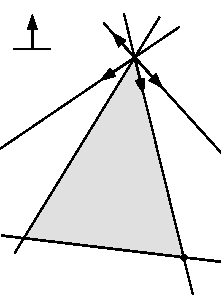
\includegraphics{chapters/chapter_4/figures/Figure1.pdf}};
		\node[right] (c) at (-1.5, 1.5) {$c$};
		\node[above] (x) at (0.5,1.7) {$x$};
		\node (y) at (1.1,-2.1) {$y$};
		\node (f) at (-0.15,1.4) {$f$};
		\node (h) at (0.35, 0.9) {$h$};
        \node (g) at (0.95, 1.3) {$g$};
        \node (-g) at (-0.3, 1.9) {$-g$};
		\node (x4=0) at (-1,1.1) {$x_4 = 0$};
		\node (x3=0) at (-1.3,-0.2) {$x_3 = 0$};
		\node (x1=0) at (-0.2,-2) {$x_1 = 0$};
		\node[right] (x2=0) at (1, -0.8) {$x_2 = 0$};
		\node[right] (x5=0) at (1, 1) {$x_5 = 0$};
	\end{tikzpicture}
	\caption{ $I_N = \braces{4,5}$ for $x$; $f$ ($x_5 > 0$) and $g$ ($x_4 >0$) are basic directions. Making $I_N = \braces{2,5}$ lead to new basic directions $h$ ($x_4 > 0$) and $-g$ ($x_2 > 0$).} \label{p1c4:fig:degenerate_basis}
\end{figure}


\section{Implementing the simplex method}

We now focus on some specific details related to alternative simplex method implementations. In a general sense, implementations of the simplex method vary in terms of how the selection of the nonbasic variables with $\overline{c}_j < 0$ that enter the basis is made. Different ways of selecting the basic variable $l = \argmin_{i \in B \mid d_i <0}\braces{-x_{B(i)}/d_{B(i)}}$ to leave the basis in case of ties might be of interest, especially in the attempt of preventing cycling.

Another important aspect related to implementations of the simplex method is how matrices are represented, its consequences on memory utilisation, and how the operations related to matrix inversion are carried out. 


\subsection{Pivot or variable selection}

The rules utilised for making choices regarding entering and leaving variables are generally referred to as \emph{pivoting rules}. However, the term most commonly used to refer to the selection of nonbasic variables to enter the basis is \emph{(simplex) pricing rules}. Recall that these are applied to choose between those variables that have favourable (negative, for minimisation) reduced costs.

% TODO: Chp4: add a bit more about these methods. Separate Devex and Steepest edge and give more details on both.
\begin{itemize}
	\item \emph{Greedy selection} (or Dantzig's rule): choose $x_j$, $j \in I_N$, with largest $|\overline{c}_j|$. Prone to cycling.
	\item \emph{Index-based order} (or Bland's rule): choose $x_j$,  $j \in I_N$, with smallest $j$. It prevents cycling but is computationally inefficient. 
%		\item The \alert{lexicographic} rule combines the two ideas above.
	\item \emph{Reduced cost pricing}: calculate $\overline{\theta}$ for all (or some) $j \in N$ and pick smallest (i.e., largest in module with negative sign) $\overline{\theta}\overline{c}_j$. Calculating the actual observed change for all nonbasic variables is too computationally expensive. Partial pricing refers to only considering a subset of the nonbasic variables to calculate $\overline{\theta}\overline{c}_j$.
	\item \emph{Devex}\footnote{P. M. J. Harris (1973), Pivot Selection Methods in the Devex LP Code, Math. Prog., 57, 341--374.} and \emph{steepest-edge}\footnote{J. Forrest \& D. Goldfarb (1992), Steepest-Edge Simplex Algorithms for LP, Math. Prog., 5, 1--28.}: most commonly used by modern implementations of the simplex method, available in professional-grade solvers. 
\end{itemize}


\subsection{The revised simplex method}

The central element in the simplex method is the calculation of the matrix $B^{-1}A_j$, from which the reduced cost vector $\overline{c}_j$, $j \in I_N$, the basic feasible direction vector $d_B$ and the step size $\overline{\theta}$ can be easily computed.

First, let us consider a more natural way of implementing the simplex method so then we can point out how the method can be revised to be more computationally efficient. We will refer to this version as the ``naive simplex''. The main differences between the naive and its revised version will be how $B^{-1}A_j$ is computed and the amount of information being carried over between iterations.

A somewhat natural way to implement the simplex method would be to store the term $p^\top = c_B^\top B^{-1}$ in an auxiliary variable by solving the linear system $p^\top B = c_B^\top$. These terms are important, as we will see later, and they are often referred to as the \emph{simplex multipliers}.

Once the simplex multipliers $p$ are available, the reduced cost $c_j$ associated with the nonbasic variable index $j \in I_N$ is simply 
%
\begin{equation*}
	\overline{c}_j = c_j - p^\top A_j.	
\end{equation*}
%
Once the column $A_j$ is selected, we can then solve a second linear system $Bu = A_j$ to determine $u = B^{-1}A_j$. 

The key observation that can yield computational savings is that we do not need to solve two linear systems. As one can notice, there is a common term between the two, the inverse of the basic matrix $B^{-1}$. If this matrix can be made available at the beginning of each iteration, then the terms $c_B^\top B^{-1}$ and $B^{-1}A_j$ can be easily and more cheaply (computationally) obtained.

For that to be possible, we need an efficient method of updating the matrix $B^{-1}$ after each iteration. To see how that can be accomplished, recall that
%
\begin{align*}
	& B = [A_{B(1)}, \dots, A_{B(m)}], \text{ and } \\ 
	& \overline{B} = [A_{B(1)}, \dots, A_{B(l-1)},A_j,A_{B(l+1)}\dots, A_{B(m)}], 
\end{align*}
%
where the $l\nth$ column $A_{B(l)}$ is precisely how the adjacent bases $B$ and $\overline{B}$ differ, with $A_j$ replacing $A_{B(l)}$ in $\overline{B}$.

We can devise an efficient manner to update $B^{-1}$ into $\overline{B}^{-1}$ utilising \emph{elementary row operations}. First, let us formally define the concept.

\begin{definition}[Elementary row operations]
	Adding a constant multiple of one row to the same or another row is called an elementary row operation.
\end{definition}

Defining elementary row operations is equivalent to devising a matrix $Q = I + D$ to premultiply $B$, where
%
\begin{equation*}
	D = \begin{cases}
		D_{ij} = \beta, \\
	    D_{i'j'} = 0 \text{ for all $i',j' \neq i,j$}.  
	\end{cases}
\end{equation*}
%
Calculating $QB = (I + D)B$ is the same as having the $j\nth$ row of $B$ multiplied by a scalar $\beta$ and then having the resulting $j\nth$ row added to the $i\nth$ row of $B$. Before we continue, let us utilise a numerical example to clarify this procedure.
%
Let
%
\begin{equation*} 
	B = \begin{bmatrix} 1 & 2 \\ 3 & 4 \\ 5 & 6
		\end{bmatrix}
\end{equation*}
%
and suppose we would like to multiply the third row by 2 and have it then added to the first row. That means that $D_{13} = 2$ and that $Q = I + D$ would be
%
\begin{equation*} 
	Q = \begin{bmatrix} 1 & & 2\\ & 1 & \\ & & 1 	\end{bmatrix}
\end{equation*}
%
Then premultiplying $B$ by $Q$ yields
%
\begin{equation*}
	QB = \begin{bmatrix} 11 & 14 \\ 3 & 4 \\ 5 & 6
		 \end{bmatrix}.
\end{equation*}	
%
As a side note, we have that $Q^{-1}$ exists since $\det(Q) = 1$. Furthermore, sequential elementary row operations $\braces{1,2,\dots, k}$ can be represented as $Q = Q_1Q_2,\dots Q_k$.

Going back to the purpose of updating $B^{-1}$ into $\overline{B}^{-1}$,  notice the following. Since $B^{-1}B = I$, each term $B^{-1}A_{B(i)}$ is the $i\nth$ unit vector $e_i$ (the $i\nth$ column of the identity matrix). That is, 
%
\begin{equation*}
	B^{-1}\overline{B} = \begin{bmatrix} \vline & & \vline & \vline & \vline & & \vline \\
		e_1 & \dots & e_{l-1} & u & e_{l+1} & \dots & e_m \\
		 \vline & & \vline & \vline & \vline & & \vline								
	\end{bmatrix} = \begin{bmatrix} 1 & & u_1 & & \\ & \ddots & \vdots &  & \\ & & u_l & & \\ & & \vdots & \ddots & \\
	& & u_m & & 1 
	 	\end{bmatrix},
\end{equation*}
%
where $u = B^{-1}A_j$. We want to define an elementary row operation matrix $Q$ such that $QB^{-1} = \overline{B}^{-1}$, or $QB^{-1}\overline{B} = I$. Therefore $Q$ will be such that the elementary row operations turn $B^{-1}\overline{B}$ into an identity matrix, i.e., that turn the vector $u$ into the unit vector $e_l$.

The main trick is that we do not need matrix multiplication to achieve it, considerably decreasing the computational burden. Instead, we can simply apply the elementary row operations, focusing only on the column $u$ and the operations required to turn it into the unit vector $e_l$. This can be achieved by:

\begin{enumerate}
	\item First, for each $i \neq l$, multiply the $l\nth$ row by $-\frac{u_i}{u_l}$ and add to the $i\nth$ row. This replaces $u_i$ with zero for all $i \in I \setminus \braces{l}$.
	\item Then, divide the $l\nth$ row by $u_l$. This replaces $u_l$ with one.
\end{enumerate}

We can restate the simplex method in its revised form. This is presented in Algorithm \ref{p1c4:alg:revised_ximplex_method}.

\begin{algorithm}[h]
	\caption{Revised simplex method} \label{p1c4:alg:revised_ximplex_method}
	\begin{algorithmic}[1] %line numbering frequency. 
	\State {\bf initialise.} Initial basis $B$, associated BFS $x$, and $B^{-1}$ are available.
	\State Calculate $p^\top = c_B^\top B^{-1}$ and $\overline{c}_j = c_j - p^\top A_j$ for $j \in I_N$.
	\While {$\overline{c}_j < 0$ for some $j \in N$} \label{p1c4:alg:opt_condition_rev} 
	    \State Choose some $j$ for which $\overline{c_j} < 0$. Calculate $u = B^{-1}A_j$. 
	    \If {$u \leq 0$} \label{p1c4:alg:unb_condition_rev}
			\State {\bf return} $z = -\infty$.		
		\Else
			\State $\overline{\theta} = \min_{i \in I_B : u_i > 0} \braces{\frac{x_{B(i)}}{u_i}}$ and $l = \argmin_{i \in I_B : u_i > 0} \braces{\frac{x_{B(i)}}{u_i}}$ 
			\State Set $x_j = \overline{\theta}$ and $x_B = x - \overline{\theta}u$.
			\State Form the matrix $[B^{-1} \,|\, u]$ and perform EROs to convert it to $[\overline{B}^{-1} \, | \, e_l]$. 
			\State Make $I_B = I_B \setminus \braces{l} \cup \braces{j}$ and $B^{-1} = \overline{B}^{-1}$. 
			\State Calculate $p^\top = c_B^\top B^{-1}$ and $\overline{c}_j = c_j - p^\top A_j$ for all $j \in I_N = J \setminus I_B$.
		\EndIf
	\EndWhile
	\State {\bf return} optimal basis $I_B$ and optimal solution $x$.
	\end{algorithmic}
\end{algorithm}

Notice that in Algorithm \ref{p1c4:alg:revised_ximplex_method}, apart from the initialisation step, no linear systems are directly solved. Instead, elementary row operations (ERO) are performed, leading to computational savings.

The key feature of the revised simplex method is a matter of representation and, thus, memory allocation savings. Algorithm \ref{p1c4:alg:revised_ximplex_method} only requires keeping in memory a matrix of the form 
%
\begin{equation*}
	\begin{bmatrix}
		p & | & p^\top b \\
		B^{-1} & | & u	
	\end{bmatrix}
\end{equation*}
%  
which, after each series of elementary row operations, yields not only $\overline{B}^{-1}$ but also the updated simplex multipliers $\overline{p}$ and $\overline{p}^\top b = c_B^\top \overline{B}^{-1}b = c_B ^\top \overline{x}_B$, which represents the objective function value of the new basic feasible solution $\overline{x} = [\overline{x}_B, \overline{x}_N]$. These savings will become obvious once we discuss the tabular (or non-revised) version of the simplex method. 

Three main issues arise when considering the efficiency of implementations of the simplex method, namely, matrix (re)inversion, representation in memory, and the use of matrix decomposition strategies.
%
\begin{itemize}
	\item \emph{Reinversion:} localised updates such as EROs have the side effect of accumulating truncation and round-off error. To correct this, solvers typically rely on periodically recalculating $B^{-1}$, which, although costly, can avoid numerical issues.
	\item \emph{Representation:} A sparse representation of $Q_n = Q_1Q_2 \dots Q_{k-1}$ can be kept instead of updating $B^{-1}$. Recall that $u = \overline{B}^{-1}A_j = QB^{-1}A_j$. For larger problems, this means a trade-off between memory allocation and the number of (sparse) matrix-matrix multiplications.
	\item \emph{Decomposition:} Decomposed (e.g., LU decomposition) forms of $B$ are used to improve efficiency in storage and the solution of the linear systems to exploit the typical sparsity of linear programming problems.  	
\end{itemize}

% TODO: Chp4: Improve this part, expanding on the points above.


\subsection{Tableau representation}

The tableau representation of the simplex method is useful as a concept presentation tool. It consists of a naive memory-intensive representation of the problem elements as they are iterated between each basic feasible solution. However, it is a helpful representation from a pedagogical standpoint and will be useful for explaining further concepts in the upcoming chapters. 

In contrast to the revised simplex method, instead of updating only $B^{-1}$, we consider the complete matrix 
%
\begin{equation*}
	B^{-1}[A ~|~ b] = \left[B^{-1}A_1, \dots, B^{-1}A_n ~|~  B^{-1}b\right].		
\end{equation*}
%
Furthermore, we adjoint a row representing the reduced cost vector $\overline{c}^\top = c^\top - c_B^\top B^{-1}A$ and the negative of the objective function value for the current basis, $ -c_Bx_B = -c_B^\top B^{-1}b$, a row often referred to as the \emph{zeroth row}. The reason why we consider the negative sign is that it allows for a simple updating rule for the zeroth row, by performing elementary row operations to make the $j^\text{th}$ element, associated with the nonbasic variable in $B$ that becomes basic in $\overline{B}$, zero.

The full tableau representation is given by

\begin{center}
	\begin{tabular}{ | c | c |} 
		\hline
		$c^\top - c_B^\top B^{-1}A$ & $-c_B^\top B^{-1}b$ \\ \hline
		$B^{-1}A$ & $B^{-1}b$ \\ \hline
	\end{tabular} 
	$\Rightarrow$ 
	\begin{tabular}{ | c  c  c | c |}
			\hline
			$\overline{c}_1$ & $\cdots$ & $\overline{c}_n$ & $-c_B x_B$ \\ \hline
			$\vline$ & & $\vline$ & $x_{B(1)}$ \\ 
			$B^{-1}A_1$ & $\cdots$ & $B^{-1}A_n$ & $\vdots$ \\
		    $\vline$ & & $\vline$ & $x_{B(m)}$ \\ \hline
	\end{tabular}
\end{center}
%

In this representation, we say that the $j^\text{th}$ column associated with the nonbasic variable to become basic is the \emph{pivot column} $u$. Notice that, since the tableau exposes the reduced costs $\overline{c}_j$, $j \in I_N$, it allows for trivially applying the greedy pricing strategy (by simply choosing the variables with a negative reduced cost with the largest absolute value). 

The $l\nth$ row associated with the basic variable selected to leave the basis is the \emph{pivot row}. Again, the tableau representation facilitates the calculation of the ratios used in choosing the basic variable $l$ to leave the basis since it amounts to simply calculating the ratios between the elements on the rightmost column and those in the pivot column, disregarding those that present entries less or equal than zero and the zeroth row. The row with the minimal ratio will be the row associated with the current basic variable leaving the basis. 

Once a pivot column and a pivot row have been defined, it is a matter of performing elemental row operations utilising the pivot row to turn the pivot column into the unit vector $e_l$ and turn to zero the respective zeroth element (recall that basic variables have zero reduced costs). This is the same as using elementary row operations using the pivot row to turn all elements in the pivot column zero, except for the \emph{pivot element} $u_l$, which is the intersection of the pivot row and the pivot column, that must be turned into one. The above highlights the main purpose of the tableau representation, which is to facilitate calculation by hand.

Notice that, as we have seen before, performing elementary row operations to convert the pivot column $u$ into $e_l$ converts $B^{-1}[A ~|~ b]$ into $\overline{B}^{-1}[A ~|~ b]$. Analogously, turning the entry associated with the pivot column $u$ in the zeroth row to zero converts $[c^\top - c_B^\top B^{-1}A \mid -c_B^\top B^{-1}b]$ into $[c^\top - c_{\overline{B}}^\top \overline{B}^{-1}A \mid -c_{\overline{B}}^\top \overline{B}^{-1}b]$.

Let us return to the paint factory example from Section \ref{section_121}, which in its standard form can be written as
%
\begin{flalign}
	\maxi z = \ & 5x_1 + 4x_2 \label{p1c1:eq:constM1}\\
	\st & 6x_1 + 4x_2  + x_3 = 24 \label{p1c1:eq:constM2}\\
	& x_1 + 2x_2 + x_4 = 6 \\
	& x_2 - x_1 + x_5 =  1 \\
	& x_2 + x_6 = 2 \\
	& x_1, \dots, x_6 \geq 0.
\end{flalign}

The sequence of tableaus for this problem is given by 

\begin{center}
	\begin{tabular}{c|cccccc|c}
		 & $x_1$ & $x_2$ & $x_3$ & $x_4$ & $x_5$ & $x_6$ & RHS \\ \hline 
		$z$  & -5 & -4 & 0 & 0 & 0 & 0 & 0   \\ \hline
	   $x_3$ &  \bf{6} & 4 & 1 & 0 & 0 & 0 & 24 \\
	   $x_4$ &  1 & 2 & 0 & 1 & 0 & 0 & 6  \\
	   $x_5$ & -1 & 1 & 0 & 0 & 1 & 0 & 1  \\
	   $x_6$ &  0 & 1 & 0 & 0 & 0 & 1 & 2  \\ \hline \hline
	\end{tabular}
	
	\begin{tabular}{c|cccccc|c}
		 & $x_1$ & $x_2$ & $x_3$ & $x_4$ & $x_5$ & $x_6$ & RHS \\ \hline 
		$z$  & 0  & -2/3& 5/6 & 0 & 0 & 0 & 20   \\ \hline
	   $x_1$ & 1  & 2/3 & 1/6 & 0 & 0 & 0 & 4 \\
	   $x_4$ & 0  & \bf{4/3} &-1/6 & 1 & 0 & 0 & 2  \\
	   $x_5$ & 0  & 5/3 & 1/6 & 0 & 1 & 0 & 5  \\
	   $x_6$ & 0  & 1 & 0 & 0 & 0 & 1 & 2  \\ \hline \hline
	\end{tabular}
	
	\begin{tabular}{c|cccccc|c}
		     & $x_1$ & $x_2$ & $x_3$ & $x_4$ & $x_5$ & $x_6$ & RHS \\ \hline 
		$z$  & 0  & 0 & 3/4 & 1/2 & 0 & 0 & 21   \\ \hline
	   $x_1$ & 1  & 0 & 1/4 & -1/2 & 0 & 0 & 3 \\
	   $x_2$ & 0  & 1 &-1/8 & 3/4 & 0 & 0 & 3/2  \\
	   $x_5$ & 0  & 0 & 3/8 &-5/4 & 1 & 0 & 5/2  \\
	   $x_6$ & 0  & 0 & 1/8 &-3/4 & 0 & 1 & 1/2  \\ \hline \hline
	\end{tabular}
\end{center}

The bold terms in the tableau represent the pivot elements at each iteration, i.e., the intersection of the pivot column and row. From the last tableau, we see that the optimal solution is $x^* = (3, 3/2)$. Notice that we applied a change in signs in the objective function coefficients, turning it into a minimisation problem; also notice that this makes the values of the objective function in the RHS column appear as positive, although it should be negative as we are in fact minimising $-5x_1 - 4x_2$, for which $x^* = (3,3/2)$ evaluates as $-21$. As we have seen, the tableau shows $-c_B x_B$, hence why the optimal tableau displays $21$ in the first row of the RHS column.


\subsection{Generating initial feasible solutions (two-phase simplex)} 

We now consider the issue of converting general linear programming problems into the standard form they are assumed to be for the simplex method. As we mentioned before, problems with constraints of the form $Ax \le b$ can be converted to standard form by simply adding nonnegative \emph{slack variables} $s \geq 0$ (recall that $b \ge 0$ can be assumed without loss of generality). In addition, we can trivially obtain an initial basic feasible solution (BFS) with $(x,s) = (0,b)$, with $B = I$, as
%
\begin{equation*}
		Ax \leq b \Rightarrow Ax + s = b.
\end{equation*}
%
Notice that this is equivalent to assuming all original problem variables (i.e., those that are not slack variables) to be initialised as zero (i.e., nonbasic) since this is a trivially available initial feasible solution. However, this approach does not work for constraints of the form $Ax \ge b$, as in this case, the transformation would take the form 
%
\begin{equation*}
	Ax \geq b \Rightarrow Ax - s = b \Rightarrow Ax - s = b.	
\end{equation*}
%
Notice that making the respective slack variable basic would yield an initial value of $-b$, making the basic solution not feasible.

For more general problems, however, this might not be possible since simply setting the original problem variables to zero might not yield a feasible solution that can be used as a BFS. To circumvent that, we rely on \emph{artificial variables} to obtain a BFS.

Let $P : \mini\braces{c^\top x : Ax = b, x \geq 0}$, which can be achieved with appropriate transformation (i.e., adding nonnegative slack to the inequality constraints) and assumed (without loss of generality) to have $b \geq 0$. Then, finding a BFS for $P$ amounts to finding a zero-valued optimal solution to the \emph{auxiliary problem}
%
\begin{align*}
	(AUX) : \mini &\sum_{i=1}^m y_i \\
	\st & Ax + y = b \\
	    & x,y \geq 0.	
\end{align*}
%
The auxiliary problem $AUX$ is formed by including one artificial variable for each constraint in $P$, represented by the vector $y$ of so-called \emph{artificial variables}. Notice that the problem is represented in a somewhat compact notation, in which we assume that all slack variables used to convert inequalities into equalities have already been incorporated in the vector $x$ and matrix $A$, with the artificial variables $y$ playing the role of ``slacks'' in $AUX$ that can be assumed to be basic and trivially yield an initial BFS for $AUX$. In principle, one does not need artificial variables for the rows in which there is a positive signed slack variable (i.e., an originally less-or-equal-than constraint), but this representation allows for compactness. 

Solving $AUX$ to optimality consists of trying to find a BFS in which the value of the artificial variables is zero since, in practice, the value of the artificial variables measures a degree of infeasibility of the current basis in the context of the original problem $P$. This means that a BFS in which the artificial variable plays no roles was found and can be used as an initial BFS for solving $P$. On the other hand, if the optimal for $AUX$ is such that some of the artificial variables are nonzero, then this implies that there is no BFS for $AUX$ in which the artificial variables are all zero, or, more specifically, there is no BFS for $P$, indicating that the problem $P$ is \emph{infeasible}.

Assuming that $P$ is feasible and $\overline{y}=0$, two scenarios can arise. The first is when the optimal basis $B$ for $AUX$ is composed only of columns $A_j$ of the original matrix $A$, with no columns associated with the artificial variables. Then $B$ can be used as an initial starting basis without any issues.

The second scenario is somewhat more complicated. Often, $AUX$ is a degenerate problem and the optimal basis $B$ may contain some of the artificial variables $y$. This then requires an additional preprocessing step, which consists of the following:
%
\begin{enumerate}
	\item[(1)] Let $A_{B(1)}, \dots, A_{B(k)}$ be the columns $A$ in $B$, which are linearly independent. We know from earlier (c.f. Theorem \ref{p1c2:thm:LI_and_bases}) that, being $A$ full-rank, we can choose additional columns $A_{B(k+1)}, \dots, A_{B(m)}$ that will span $\reals^{m}$.
	\item[(2)] Select the $l\nth$ artificial variable $y_l = 0$ and select a component $j$ in the $l\nth$ row with nonzero $B^{-1}A_j$ and use elementary row operations to include $A_j$ in the basis. Repeat this $m-k$ times.
\end{enumerate}

The procedure is based on several ideas we have seen before. Since $\sum_{i=1}^m y_i$ is zero at the optimal, there must be a BFS in which the artificial variables are nonbasic (which is what (1) is referring to). Thus, step (2) can be repeated until a basis $B$ is formed and includes none of the artificial variables. 

Some interesting points are worth highlighting. First, notice that $B^{-1}A_{B(i)} = e_i$, $i=1, \dots, k$. Since $k < l$, the $l\nth$ component of each of these vectors is zero and will remain so after performing the elementary row operations. In turn, the $l\nth$ entry of $B^{-1}A_j$ is not zero, and thus $A_j$ is linearly independent to $A_{B(1)}, \dots, A_{B(k)}$. 

However, it might be so that we find zero elements in the $l\nth$ row. Let $g$ be the $l\nth$ row of $B^{-1}A$ (i.e., the entries in the tableau associated with the original problem variables). If $g$ is the null vector, then $g_l$ is zero, and the procedure fails. However, note that $g^\top A = 0 $ $= g^\top Ax = g^\top b$, implying that $g^\top Ax = g^\top b$ is \emph{redundant} can be removed altogether. 

This process of generating initial BFS is often referred to as \emph{Phase I} of the two-phase simplex method. \emph{Phase II} consists of employing the simplex method as we developed it, utilising the BFS found in Phase I as a starting basis.


\section{Column geometry of the simplex method}

Let us try to develop a geometrical intuition on why it is so that the simplex method is remarkably efficient in practice. As we have seen in Theorem \ref{p1c4:thm:convergece_simplex}, although the simplex method is guaranteed to converge, the total number of steps the algorithm might need to take before convergence grows exponentially with the number of variables and constraints, since the number of steps depends on the number of vertices of the polyhedral set that represents the feasible region of the problem. 

However, it turns out that, in practice, the simplex method typically requires $O(m)$ iterations (recall that $m$ is the number of rows in the matrix $A$), being one of the reasons why it has experienced tremendous success and is one of the most mature and reliable methods when it comes to optimisation. 

To develop a geometrical intuition on why this is the case, let us first consider an equivalently reformulated problem $P$:
%
\begin{align*}
	P : \mini & z           \\
	\st & Ax = b        \\
	& c^\top x = z      \\	
	& \sum_{j=1}^nx_j=1 \\
	& x \geq 0.
\end{align*}
% 
In this reformulation, we make the objective function an auxiliary variable, so it can be easily represented on a real line at the expense of adding an additional constraint $c^\top x = z$. Furthermore, we normalise the decision variables so they add to one (notice that this implies a bounded feasible set). Notice that problem $P$ can be equivalently represented as  
%
\begin{align*}
	P : \mini & z     \\
	\st & x_1\begin{bmatrix}
		A_1 \\
		c_1
	\end{bmatrix} + x_2\begin{bmatrix}
		A_2 \\
		c_2
	\end{bmatrix} + \dots +
	x_n\begin{bmatrix}
		A_n \\
		c_n
	\end{bmatrix} = \begin{bmatrix}
		b \\
		z
	\end{bmatrix}\\
	& \sum_{j=1}^nx_j=1 \\
	& x \geq 0.
\end{align*}
% 
This second formulation exposes one interesting interpretation of the problem. Solving $P$ is akin to finding a set of weights $x$ that makes a convex combination (c.f. Definition \ref{p1c2:def:convex_combination_hull}) of the columns of $A$ such that it constructs (or matches) $b$ in a way that the resulting combination of the respective components of the vector $c$ is minimised. Now, let us define some nomenclature that will be useful in what follows.
%
\begin{definition}[$k$-dimensional simplex] \label{p1c4:def:simplex}
	A collection of vectors $y_1, \dots, y_{k+1}$ are affinely independent if $k \leq n$ and $y_1 - y_{k+1}, \dots, y_{k} - y_{k+1}$ are linearly independent. The convex hull of $k+1$ affinely independent vectors is a $k$-dimensional simplex.
\end{definition}
%
Definition \ref{p1c4:def:simplex} is precisely the inspiration for the name of the simplex method. We know that only $m+1$ components of $x$ will be different than zero since that is the number of constraints we have and, thus, the size of a basis in this case. Thus, a BFS is formed by $m+1$ $(A_i, 1)$ columns, which in turn are associated with $(A_i,c_i)$ basic points. 

Figure \ref{p1c4:fig:column_geometry} provides an illustration of the concept. In this, we have that $m=2$, so each column $A_j$ represents a point in a two-dimensional plane. Notice that a basis requires three points $(A_i,c_i)$ and forms a 3-simplex. A BFS is a selection of three points $(A_i,c_i)$ such that $b$, also illustrated in the picture, can be formed by a convex combination of the $(A_i,c_i)$ forming the basis. This will be possible if $b$ happens to be inside the 3-simplex formed by these points. For example, in Figure \ref{p1c4:fig:column_geometry}, the basis formed by columns $\braces{2,3,4}$ is a BFS, while the basis $\braces{1,2,3}$ is not.

\begin{figure}[h]
	\begin{tikzpicture}
		\node (pic) at (0,0) {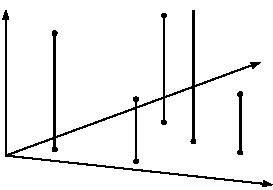
\includegraphics{chapters/chapter_4/figures/Figure2.pdf}}; 
		\node (A1) at (-1.1, -0.9) {$A_1$};
		\node (A1c1) at (-1.4, 1.3) {$(A_1, c_1)$};
		\node (A2) at (0.3, -1.1) {$A_2$};
		\node (A2c2) at (-0.4, 0.2) {$(A_2, c_2)$};
		\node (A3c3) at (0.1, 1.6) {$(A_3, c_3)$};
		\node (A3) at (0.7, -0.5) {$A_3$};
     	\node (A4) at (2, -1) {$A_4$};
		\node (A4c4) at (2.4, 0) {$(A_4, c_4)$};
     	\node (b) at (1.15, -0.8) {$b$};
    	\node (z) at (-2.4, 1.4) {$z$};    
	\end{tikzpicture}
	\caption{A solution $x$ is a convex combinations of $(A_i,c_i)$ such that $Ax= b$.} \label{p1c4:fig:column_geometry}
\end{figure}	 

We now can add a third dimension to the analysis representing the value of $z$. For that, we will use Figure \ref{p1c4:fig:column_geometry_3d}. As can be seen, each selection of basis creates a tilt in the three-dimensional simplex, such that the point $b$ is met precisely at the height corresponding to its value in the $z$ axis. This allows us to compare bases according to their objective function value. And, since we are minimising, we would like to find the basis that has its respective simplex crossing $b$ at the lowermost point.

\begin{figure}[H]
	\begin{tikzpicture}
%			\draw[help lines] (-2,-3) grid (2,3);
		\node (pic) at (0,0) {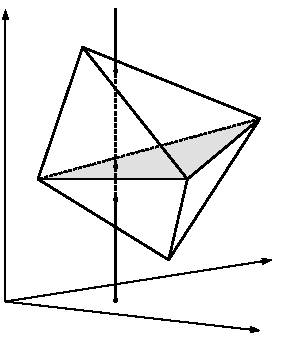
\includegraphics{chapters/chapter_4/figures/Figure3.pdf}}; 
		\node (z) at (-2.5, 2.6) {$z$};
		\node (F) at (-2, -0.1) {$F$};
		\node (G) at (-0.7, -0.5) {$G$};
        \node (H) at (-0.1, 0.1) {$H$};
        \node (I) at (-0.25, 1.55) {$I$};
		\node (B) at (-1, 2.4) {$B$};
		\node (C) at (2, 1.2) {$C$};
		\node (D) at (0.95, -0.3) {$D$};
      	\node (E) at (0.7, -1.55) {$E$};
      	\node (b) at (-0.2, -2.2) {$b$};   		   		
	\end{tikzpicture}
	\caption{A solution $x$ is a convex combinations of $(A_i,c_i)$ such that $Ax= b$.} \label{p1c4:fig:column_geometry_3d}
\end{figure}	

Notice that in Figure \ref{p1c4:fig:column_geometry_3d}, although each facet is a basic simplex, only three are feasible ($BCD$, $CDF$, and $DEF$). We can also see what one iteration of the simplex method does under this geometrical interpretation. Moving between adjacent basis means that we are replacing one vertex (say, $C$) with another (say, $E$) considering the potential for a decrease in value in the $z$ axis (represented by the difference between points $H$ and $G$ onto the $z$ axis). You can also see the notion of pivoting: since we are moving between adjacent bases, two successive simplexes share an edge in common. Consequently, they pivot around that edge (think about the movement of the edge $C$ moving to the point $E$ while the edge $\overline{DF}$ remains fixed).

\begin{figure}[h]
	\begin{tikzpicture}
%			\draw[help lines] (-2,-3) grid (2,3);
		\node (pic) at (0,0) {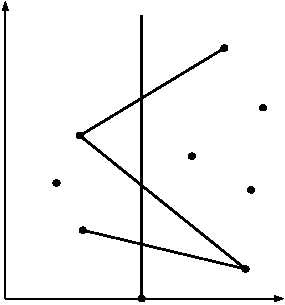
\includegraphics{chapters/chapter_4/figures/Figure4.pdf}}; 
		\node (1) at (1.8, 0.8) {$1$};
		\node (6) at (1.65, 1.8) {$6$}; 		   		
		\node (3) at (-1.3, 0.3) {$3$}; 		   		
		\node (2) at (1.1, -0.05) {$2$};
		\node (7) at (1.6, -0.6) {$7$};
		\node (4) at (-1.2, -0.5) {$4$};
		\node (8) at (-1.25, -1.3) {$8$};
		\node (5) at (2, -2) {$5$};
		\node (b) at (0, -2.7) {$b$};
	\end{tikzpicture}
	\caption{Pivots from initial basis $[A_3, A_6]$ to $[A_3, A_5]$ and to the optimal basis $[A_8, A_5]$} \label{p1c4:fig:column_geometry_projection}
\end{figure}		
 
Now we are ready to provide an insight into why the simplex method is often so efficient. The main reason is associated with the ability that the method possesses of skipping bases in favour of those with most promising improvement. To see that, consider Figure \ref{p1c4:fig:column_geometry_projection}, which is a 2-dimensional schematic projection of Figure \ref{p1c4:fig:column_geometry_3d}. By using the reduced costs to guide the choice of the next basis, we tend to choose the steepest of the simplexes that can provide reductions in the objective function value, which has the side effect of allowing for skipping several bases that would have to be otherwise considered. This creates a ``sweeping effect'', which allows the method to find optimal solutions in fewer pivots than vertices. Clearly, this can be engineered to be prevented, as there are examples purposely constructed to force the method to consider every single vertex, but the situation illustrated in Figure \ref{p1c4:fig:column_geometry_projection} is by far the most common in practice.  

% TODO: Chp4: include a discussion on dual plane, to make more concrete the relationship between the z axis and reduced costs.

 \vfill
\pagebreak
\section{Exercises}

\subsection*{Exercise 4.1: Properties of the simplex algorithms}
Consider the simplex method applied to a standard form minimization problem, and assume that the rows of the matrix $A$ are linearly independent. For each of the statements that follow, give either a proof or a counter example.
\begin{itemize}
\item[(a)] An iteration of the simplex method might change the feasible solution while leaving the cost unchanged.
%\item[(b)] A variable that has just left the basis cannot re-enter in the very next iteration.
\item[(b)] A variable that has just entered the basis cannot leave in the very next iteration.
\item[(c)] If there is a non-degenerate optimal basis, then there exists a unique optimal basis.
%\item[(e)] If $\bf x$ is an optimal solution found by the simplex method, no more than $m$ of its components can be positive, where $m$ is the number of equality constraints.
\end{itemize}

\subsection*{Exercise 4.2: The simplex method}
Consider the problem
%
\begin{align*}
	\maxi & 40x_1 + 60 x_2   \\
	\st   & 2x_1 + x_2 \le 7 \\
		  & x_1 + x_2 \le 4  \\
		  & x_1 + 3x_2 \le 9 \\
		  & x_1, x_2 \ge 0.
\end{align*}

A feasible point for this problem is $(x_1,x_2)=(0,3)$. Formulate the problem as a minimisation problem in standard form and verify whether or not this point is optimal. If not, solve the problem by using the simplex method.

\subsection*{Exercise 4.3: Solving a tableau}
\renewcommand{\arraystretch}{1.1}
\setlength{\tabcolsep}{8pt}
Consider a linear programming problem in standard form, described in terms of the following tableau:
%
\begin{center}
\begin{tabular}{c|ccccccc|c}
  & $x_1$ & $x_2$ & $x_3$ & $x_4$ & $x_5$ & $x_6$ & $x_7$ & RHS\\
\hline
 $z$        &$0$ & $0$ & $0$ & $\delta$ & 3 & $\gamma$ & $\xi$ & 0\\
\hline
$x_2$   &  0 & 1 & 0 & $\alpha$ & 1 & 0      &  3 & $\beta$ \\
$x_3$   &  0 & 0 & 1 & -2\,\,       & 2 & $\eta$ & -1 &  2 \\
$x_1$   &  1 & 0 & 0 &  0       &-1\,\, & 2      &  1 &  3 \\ \hline
\end{tabular}
\end{center}
%
The entries $\alpha$, $\beta$, $\gamma$, $\delta$, $\eta$ and $\xi$ in the tableau are unknown parameters. Furthermore, let $B$ be the basis matrix corresponding to having $x_2$, $x_3$, and $x_1$ (in that order) be the basic variables. For each one of the following statements, find the ranges of values of the various parameters that will make the statement to be true.
\begin{itemize}
\item[(a)] Phase II of the Simplex method can be applied using this as an initial tableau.
\item[(b)] The corresponding basic solution is feasible, but we do not have an optimal basis.
\item[(c)] The corresponding basic solution is feasible and the first Simplex iteration indicates that the optimal cost is $-\infty$.
\item[(d)] The corresponding basic solution is feasible, $x_6$ is a candidate for entering the basis, and when $x_6$ is the entering variable, $x_3$ leaves the basis.  
\item[(e)] The corresponding basic solution is feasible, $x_7$ is a candidate for entering the basis, but if it does, the objective value remains unchanged.
\end{itemize}

\subsection*{Exercise 4.4: Two-phase simplex method}
Solve the problem below using the two-phase simplex method. What is your conclusion about the feasibility of the problem? Verify your results by drawing the feasible region.
%
\begin{align*}
	\maxi & 5x_1 + x_2 			\\
	\st   & 2x_1 + x_2 \geq 5   \\
		  & x_2 \geq 1 			\\
		  & 2x_1 + 3x_2 \leq 12 \\
		  & x_1, x_2 \geq 0.
\end{align*}




	
		
	\chapter{Linear Programming Duality - Part I} \label{chapter_5}
	\section{Formulating duals}

In this chapter, we will discuss the notion of duality in the context of linear programming problems. Duality can be understood as a toolbox of technical results that makes available a collection of techniques and features that can be exploited to both further understand characteristics of the optimal solution and to devise specialised methods for solving linear programming problems.


\subsection{Motivation}

Let us define the notation we will be using throughout the next chapters. As before, let $c \in \reals^n$, $b \in \reals^m$, $A \in \reals^{m \times n}$, and $P$ be the standard form linear programming problem
%
\begin{align*}
	(P) : \mini \ & c^\top x \\
	\st 	  & Ax = b \\
		  & x \geq 0,   
\end{align*}
%
which we will refer to as the \emph{primal} problem. In mathematical programming, we say that a constraint has been \emph{relaxed} if it has been removed from the set of constraints. With that in mind, let us consider a \emph{relaxed} version of $P$, where $Ax = b$ is replaced with a \emph{violation penalty} term $p^\top (b - Ax)$. This leads to the following problem:
%
\begin{equation*}
	g(p) = \mini_{x \geq 0} \braces{c^\top x + p^\top (b - Ax)},
\end{equation*}
%
which has the benefit of not having equality constraints explicitly represented, but only implicit by means of a penalty term. This term is used to penalise the infeasibility of the constraints in the attempt to steer the solution of the relaxed problem towards the solution to $P$. Recalling that our main objective is to solve $P$, we are interested in the values (or prices, as they are often called) for $p \in \reals^m$ that make $P$ and $g(p)$ equivalent.

Let $\overline{x}$ be the optimal solution to $P$. Notice that, for any $p \in \reals^m$, we have that
%
\begin{equation*}
	g(p) = \mini_{x \geq 0} \braces{c^\top x + p^\top (b - Ax)} \leq c^\top \overline{x} +  p^\top (b - A\overline{x}) = c^\top \overline{x},   
\end{equation*}
%
i.e., $g(p)$ is a \emph{lower bound} on the optimal value $c^\top \overline{x}$. The inequality holds because, although $\overline{x}$ is optimal for $P$, it might not be optimal for $g(p)$ for an arbitrary vector $p$. The rightmost equality is a consequence of $\overline{x} \in P$, i.e., the feasibility of $\overline{x}$ implies that $A\overline{x} = b$.

We can use an optimisation-based approach to try to find an optimal lower bound, i.e., the tightest possible lower bound for $P$. This can be achieved by solving the \emph{dual problem} $D$ formulated as 
%
\begin{equation*}
	(D) : \maxi_p g(p).
\end{equation*}
%
Notice that $D$ is an unconstrained problem to which a solution proves the \emph{tightest} lower bound on $P$ (say, at $\overline{p}$). Also, notice how the function $g(p) : \reals^m \to \reals$ has embedded on its evaluation the solution of a linear programming problem with $x \in \reals^n$ as decision variables for a fixed $p$, which is the argument given to the function $g$. %This is a new concept at this point that often is a source of confusion. 

We will proceed in this chapter developing the analytical framework that allows us to pose the key result in duality theory, which states that 
%
\begin{equation*}
	g(\overline{p}) = c^\top \overline{x}.	
\end{equation*}
%
That is, we will next develop the results that guarantee the equivalence between primal and dual representations. This will be useful for interpreting properties associated with the optimal primal solution $\overline{x}$ from the associated optimal prices $\overline{p}$. Furthermore, we will see in later chapters that linear programming duality can be used as a framework for replacing constraints with equivalent representations, which is a useful procedure in many settings, including developing alternative solution strategies also based on linear programming. 


\subsection{General form of duals}

Now, let us focus on developing a formulation for dual problems that is based on linear programming as well. Using the definition of $D$, we notice that
%
\begin{align*}
	g(p) = \ & \mini_{x \geq 0}  \braces{c^\top x + p^\top (b - Ax)}	\\
	= \ & p^\top b + \mini_{x \geq 0}  \braces{c^\top x - p^\top Ax}    \\
    = \ & p^\top b + \mini_{x \geq 0}  \braces{(c^\top - p^\top A)x}.  
\end{align*} 
%
As $x \ge 0$, the rightmost problem can only be bounded if $(c^\top - p^\top A) \ge 0$. This gives us a linear constraint that can be used to enforce the existence of a solution for 
%
\begin{equation*}
	\mini_{x \geq 0}  \braces{(c^\top - p^\top A)x}.
\end{equation*}
%
With that in mind, we can equivalently reformulate $D$ as
%
\begin{align*}
	(D) : \maxi \ & p^\top b \\
	\st 	  & p^\top A \leq c^\top.
\end{align*}	
%
Notice that $D$ is a linear programming problem with $m$ variables (one per constraint of the primal problem $P$) and $n$ constraints (one per variable of $P$). As you might suspect, if you were to repeat the analysis, looking at $D$ as the ``primal'' problem, you would end with a dual that is exactly $P$. For this to become more apparent, let us first define more generally the rules that dictate what kind of dual formulations are obtained for different types of primal problems in terms of their original (i.e., not in standard) form. 

In the more general case, let $P$ be defined as
%
\begin{align*}
	(P) : \mini \ & c^\top x \\
	\st 	  & Ax \geq b.  
\end{align*}
%
Notice that the problem $P$ can be equivalently reformulated as
%
\begin{align*}
	(P) : \mini \ & c^\top x \\
	\st & Ax - s = b \\
	& s \geq 0.
\end{align*}
%
Let us focus on the constraints in the reformulated version of $P$, which can be written as
%
\begin{equation*}
	[A \mid -I] \begin{bmatrix} x \\ s \end{bmatrix} = b. 
\end{equation*}
%
We will apply the same procedure as before, being our constraint matrix $[A \mid -I]$ in place of $A$ and $[x \mid s]^\top$ our vector of variables, in place of $x$. Using analogous arguments, we now require that $c^\top - p^\top A = 0$, so $g(p)$ is finite. Notice that this is a slight deviation from before, but in this case, we have that $x \in \reals^n$, so $c^\top - p^\top A = 0$ is the only condition that allows the inner problem in $g(p)$ to have a finite solution. Then, we obtain the following conditions to be imposed to our dual linear programming formulation
%
\begin{align*}
	&p^\top [A \mid -I] \leq [c^\top \mid 0^\top]  \\
	&c^\top - p^\top A = 0, 
\end{align*}
%
Combining them all and redoing the previous steps for obtaining a dual formulation, we arrive at 
%
\begin{align*}
	(D) : \maxi \ & p^\top b  \hspace{1.5cm}\\ 
	\st & p^\top A = c^\top \\
	& p \geq 0.
\end{align*}

Notice how the change in the type of constraints in the primal problem $P$ lead to additional nonnegative constraints in the dual variables $p$. Similarly, the absence of explicit nonnegativity constraints in the primal variables $x$ lead to equality constraints in the dual problem $D$, as opposed to inequalities. 

Table \ref{p1c5:tab:primal-dual_conversion} provides a summary which allows one to identify the resulting formulation of the dual problem based on the primal formulation, in particular regarding its type (minimisation or maximisation), constraint types and variable domains.

\begin{table}[h]
	\begin{tabular}{|c|c|} \hline
		{\bf Primal (dual)} & {\bf Dual (primal)} \\ \hline
		 minimise & maximise \\
		Independent terms  & Obj. function coef.  \\
		Obj. function coef.  & Independent terms  \\
		$i$-th row of constraint coef. & $i$-th column of constraint coef. \\
		$i$-th column of constraint coef. & $i$-th row of constraint coef. \\ \hline
		{\bf Constraints} & {\bf Variables} \\ \hline
		$\geq$ & $\geq 0$ \\
		$\leq$ & $\leq 0$ \\
		$=$ & $\in \reals$ \\ \hline
		{\bf Variables} & {\bf Constraints} \\ \hline
		$\geq 0$ & $\leq$ \\
		$\leq 0$ & $\geq$ \\
		$\in \reals$ & $=$ \\ \hline
	\end{tabular}
	\caption{Primal-dual conversion table} \label{p1c5:tab:primal-dual_conversion}
\end{table}

For converting a minimisation primal problem into a (maximisation) dual, one must read the table from left to right. That is, the independent terms ($b$) become the objective function coefficients, greater or equal constraints become nonnegative variables, and so forth. However, if the primal problem is a maximisation problem, the table must be read from right to left. For example, in this case, less-or-equal-than constraints would become nonnegative variables instead, and so forth. It takes a little practice to familiarise yourself with this table, but it is a really useful resource to obtain dual formulations from primal problems.

One remark to be made at this point is that, as is hopefully clearer now, the conversion of primal problems into duals is symmetric, meaning that reapplying the rules in Table \ref{p1c5:tab:primal-dual_conversion} would take you from the obtained dual back to the original primal. This is a property of linear programming problems called being \emph{self dual}. Another remark is that equivalent reformulations made in the primal lead to equivalent duals. Specifically, transformations that replace variables $x \in \reals$ with $x^+ - x^-$, where $x^+, x^- \geq 0$, introduce nonnegative slack variables, or remove redundant constraints all lead to equivalent duals. 

For example, recall that the dual formulation for the primal problem 
%
\begin{align*}
	(P) : \mini \ & c^\top x \\
	\st &Ax \geq b \\
	&x \in \reals^n
\end{align*}
%
is given by
%
\begin{align*}
	(D) : \maxi \ & p^\top b \\
	\st &p \geq 0 \\
	&p^\top A = c^\top. 
\end{align*}
%
Now suppose we equivalently reformulate the primal problem to become
\begin{align*}
	(P') : \mini \ & c^\top x + 0^\top s \\
	\st &A x - s = b \\
	&x \in \reals^n, s \geq 0.
\end{align*}
%
Then, using Table \ref{p1c5:tab:primal-dual_conversion}, we would obtain the following dual formulation, which is equivalent to $D$
\begin{align*}
	(D') : \maxi \ & p^\top b \\
	\st &p \in \reals^m \\
	&p^\top A = c^\top \\
	-&p \leq 0.
\end{align*}
%
Analogously, suppose we were to equivalently reformulate $P$ as 
%
\begin{align*}
	(P'') : \mini \ & c^\top x^+ - c^\top x^- \\
	\st &Ax^+ - Ax^- \geq b \\
	&x^+ \geq 0, x^- \geq 0.
\end{align*}
%
Then, the dual formulation for $P''$ would be 
%
\begin{align*}
	(D'') : \maxi \ & p^\top b \\
	\st &p \geq 0 \\
	&p^\top A \leq c \\
	-&p^\top A \leq -c^\top,
\end{align*}
%
which is also equivalent to $D$.


\section{Duality theory}

We will now develop the technical results associated with duality that will be the kingpin for its use as a framework for devising solution methods and interpreting optimal solution properties. 

\subsection{Weak duality}

Weak duality is the property associated with the bounding nature of dual feasible solutions. This is stated in Theorem \ref{p1c5:thm:weak_duality}.

\begin{theorem}[Weak duality] \label{p1c5:thm:weak_duality}
		Let $x$ be a feasible solution to $(P) : \mini\braces{c^\top x : Ax = b, x \geq 0}$ and $p$ be a feasible solution to $(D) : \maxi\braces{p^\top b : p^\top A \leq c^\top}$, the dual problem of $P$. Then $c^\top x \geq p^\top b$.
\end{theorem}

\begin{proof}
	Let $I = \braces{i}_{i=1}^m$ and $J = \braces{j}_{j=1}^n$. For any $x$ and $p$, define
%
	  	\begin{equation*}
			u_i = p_i (a_i^\top x - b_i) \text{ and }
			v_j = (c_j - p^\top A_j)x_j.	
		\end{equation*}
%
	Notice that $u_i \geq 0$ for $i \in I$ and $v_j \geq 0$ for $j \in J$, since each pair of terms will have the same sign (you can see that from Table \ref{p1c5:tab:primal-dual_conversion} and assuming $x_j$ to be the dual variable associated with $p^\top A \leq c^\top$).  Thus, we have that
%
	\begin{equation*}
		0 \leq \sum_{i \in I} u_i + \sum_{j \in J} v_j = [p^\top Ax - p^\top b] + [c^\top x - p^\top Ax] = c^\top x - p^\top b. \qedhere
	\end{equation*}
%
\end{proof}

Let us also pose some results that are direct consequences of Theorem \ref{p1c5:thm:weak_duality}, which are summarised in Corollary \ref{p1c5:cor:weak_duality}.

\begin{corollary}[Consequences of weak duality]\label{p1c5:cor:weak_duality}
	The following are immediate consequences of Theorem \ref{p1c5:thm:weak_duality}:
	\begin{enumerate}
		\item[(1)] If the optimal value of $P$ is $-\infty$ (i.e., $P$ is unbounded), then $D$ must be infeasible;
		\item[(2)] if the optimal value of $D$ is $\infty$ (i.e., $D$ is unbounded), then $P$ must be infeasible;
		\item[(3)] let $x$ and $p$ be feasible to $P$ and $D$, respectively. Suppose that $p^\top b = c^\top x$. Then $x$ is optimal to $P$ and $p$ is optimal to $D$.
	\end{enumerate}
\end{corollary}

\begin{proof} 
	By contradiction, suppose that $P$ has optimal value $-\infty$ and that $D$ has a feasible solution $p$. By weak duality, $p^\top b \leq c^\top x = -\infty$, i.e., a contradiction. Part (2) follows a symmetric argument.
	
	Part (3): let $\overline{x}$ be an alternative feasible solution to $P$. From weak duality, we have $c^\top \overline{x} \geq p^\top b = c^\top x$, which proves the optimality of $x$. The optimality of $p$ follows a symmetric argument.
\end{proof}

Notice that Theorem \ref{p1c5:thm:weak_duality} provides us with a bounding technique for any linear programming problem. That is, for a given pair of primal and dual feasible solutions, $\overline{x}$ and $\overline{p}$, respectively, we have that 
%
\begin{equation*}
	 \overline{p}^\top b \le c^\top x^* \le c^\top \overline{x},
\end{equation*}
%
where $c^\top x^*$ is the optimal objective function value.

Corollary \ref{p1c5:cor:weak_duality} also provides an alternative way of identifying infeasibility by means of linear programming duals. One can always use the unboundedness of a given element of a primal-dual pair to state the infeasibility of the other element in the pair. That is, an unbounded dual (primal) implies an infeasible primal (dual). However, the reverse statement is not as conclusive. Specifically, an infeasible primal (dual) does not necessarily imply that the dual (primal) is unbounded, but does imply it to be \emph{either} infeasible or unbounded.   


\subsection{Strong duality}

This bounding property can also be used as a certificate of optimality, in case they match in value. This is precisely the notion of \emph{strong duality}, a property that is inherent to linear programming problems. This is stated in Theorem \ref{p1c5:thm:strong_duality}.

\begin{theorem}[Strong duality]\label{p1c5:thm:strong_duality}
	If $(P) : \mini\braces{c^\top x : Ax = b, x \geq 0}$ has an optimal solution, so does its dual $(D) : \maxi\braces{p^\top b : p^\top A \leq c^\top}$ and their respective optimal values are equal.
\end{theorem}

\begin{proof}
	Assume $P$ is solved to optimality, with optimal solution $x$ and basis $B$. Let $x_B = B^{-1}b$. At the optimal, the reduced costs are $c^\top - c_B^\top B^{-1}A \geq 0$. Let $p = c_B^\top B^{-1}$. We then have $p^\top A \leq c^\top$, which shows that $p$ is feasible to $D$. Moreover,
%
	\begin{equation} \label{p1c5:eq:primal-dual}
		p^\top b = c_B^\top B^{-1}b = c_B^\top x_B = c^\top x,			
	\end{equation}
%
which, in turn, implies the optimality of $p$ (cf. Corollary \ref{p1c5:cor:weak_duality} (3)). \qedhere
\end{proof}

The proof of Theorem \ref{p1c5:thm:strong_duality} reveals something remarkable relating the simplex method and the dual variables $p$. As can be seen in \eqref{p1c5:eq:primal-dual}, for any primal feasible solution $x$, an associated dual (not necessarily) feasible solution $p$ can be immediately recovered. If the associated dual solution is also feasible, then Theorem \ref{p1c5:thm:strong_duality} guarantees that optimality ensues.

This means that we can interchangeably solve either a primal or a dual form of a given problem, considering aspects related to convenience and computational ease. This is particularly useful in the context of the simplex method since the prices $p$ are readily available as the algorithm progresses. In the next section, we will discuss several practical uses of this relationship in more detail. For now, let us halt this discussion for a moment and consider a geometrical interpretation of duality in the context of linear programming.


\section{Geometric interpretation of duality}

Linear programming duality has an interesting geometric interpretation that stems from the much more general framework of Lagrangian duality (of which linear programming duality is a special case) and its connection to optimality conditions, topics that will be further explored in Part \ref{part_2}. For now, let us focus on how linear programming duality can be interpreted in the context of ``balancing forces''. 

First, let $\overline{x}$ be the optimal solution of primal problem $P$ in the form
%
\begin{align*}
	(P) : \mini \ & c^\top x \\
	\st & a_i^\top x \geq b_i, \ \forall i \in I.
\end{align*}
%
Imagine that there is a particle within the polyhedral set representing the feasible region of $P$ and that this particle is subjected to a force represented by the vector $-c$. Notice that this is equivalent to minimising the function $z = c^\top x$ within the polyhedral set $\braces{a_i^\top x \geq b_i}_{i\in I}$ representing the feasible set of $P$. Assuming that the feasible set of $P$ is bounded in the direction $-c$, this particle will eventually come to a halt after hitting the ``walls'' of the feasible set, at a point where the pulling force $-c$ and the reaction of these walls reach an equilibrium. We can think of $\overline{x}$ as this stopping point. This is illustrated in Figure \ref{p1c5:fig:duality_geometry}.

\begin{figure}[h]
	\begin{tikzpicture}
		\node (fig) at (0,0){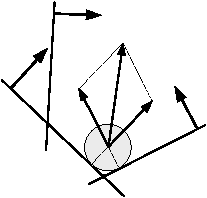
\includegraphics[scale=1]{chapters/chapter_5/figures/Figure1}};
		\node (c) at (0.3,1.1) {$c$};
		\node (a1) at (-1.2,1.0) {$a_1$};					
		\node (a2) at (1.65,0.1) {$a_2$};					
		\node (a3) at (-0.2,1.65) {$a_3$};
		\node (p1a1) at (0.7,0.2) {\small $p_1a_1$};					
		\node (p2a2) at (-0.4,0.4) {\small $p_2a_2$};				
		\node (x) at (0,-1.55) {\small $\overline{x}$};						
	\end{tikzpicture}			
	\caption{A geometric representation of duality for linear programming problems} \label{p1c5:fig:duality_geometry}	
\end{figure}

We can then think of the dual variables $p$ as the multipliers applied to the normal vectors associated with the hyperplanes (i.e., the walls) that are in contact with the particle to achieve this equilibrium. Hence, these multipliers $p$ will be such that
%
\begin{equation*}
c = \sum_{i \in I}p_ia_i, \text{ for some } p_i \geq 0, i \in I,	
\end{equation*}
%
which is precisely the dual feasibility condition (i.e., constraint) associated with the dual of $P$, given by
%
\begin{equation*}
	D : \maxi \braces{p^\top b : p^\top A = c, p \geq 0}.	
\end{equation*}
%
And, dual feasibility, as we seen before, implies the optimality of $\overline{x}$. 


\subsection{Complementary slackness}

One point that must be noticed is that, for the constraints that are not active at the optimal point $\overline{x}$ (i.e., the walls that are not exerting resistance to the particle at the equilibrium point), the multipliers $p$ must be set to zero. That is, we have that
%
\begin{equation*}
	p^\top b  = \sum_{i \in I} p_ib_i = \sum_{i \in I} p_i(a_i^\top\overline{x}) = c^\top \overline{x},	
\end{equation*}
%
which again implies the optimality of $p$ (cf. Corollary \ref{p1c5:cor:weak_duality} (3)). This geometrical insight leads to another key result for linear programming duality, which is the notion of \emph{complementary slackness}.

\begin{theorem}[Complementary slackness]\label{p1c2:thm:complemetarity_slackness}
	Let $x$ be a feasible solution for 
	%
	\begin{equation*}
		(P) : \mini\braces{c^\top x : Ax = b, x \geq 0}	
	\end{equation*}
	%
	and $p$ be a feasible solution for 
	%
	\begin{equation*}
		(D) : \maxi\braces{p^\top b : p^\top A \leq c^\top}. 	
	\end{equation*}
	%
	The vectors $x$ and $p$ are optimal solutions to $P$ and $D$, respectively, if and only if
	$p_i(a_i^\top x - b_i) = 0, \forall i \in I$, and $(c_j - p^\top A_j)x_j = 0, \, \forall j \in J$. 
\end{theorem}

\begin{proof} 
	From the proof of Theorem \ref{p1c5:thm:weak_duality} and with Theorem \ref{p1c5:thm:strong_duality} holding, we have that 
%
	\begin{equation*}
		p_i(a_i^\top x - b_i) = 0, \forall i \in I, \text{ and } 	
	(c_j - p^\top A_j)x_j = 0, \, \forall j \in J.
	\end{equation*}
%
	In turn, if these hold, then $x$ and $p$ are optimal (cf. Corollary \ref{p1c5:cor:weak_duality} (3)). 
\end{proof}

Theorem \ref{p1c2:thm:complemetarity_slackness} exposes an important feature related to optimal solutions. Notice that $a_i^\top x - b_i$ represents the slack value of constraint $i \in I$. Thus, under the assumption of nondegeneracy, $p_i(a_i^\top x - b_i) = 0, \forall i \in I$ implies that for each constraint $i \in I$, either the dual variable $p_i$ associated with constraint is zero, or the associated slack value $a_i^\top x - b_i$ is zero. 

For nondegenerate basic feasible solutions (BFS) (i.e., $x_j > 0$, $\forall j \in I_B$, where $I_B$ is the set of basic variable indices), complementary slackness determines a \emph{unique} dual solution. That is
%
\begin{equation*}
	(c_j - p^\top A_j)x_j = 0, \text{ which yields } c_j = p^\top A_j, \, \forall j \in I_B,
\end{equation*}
%
which has a unique solution $p^\top = c_B^\top B^{-1}$, as the columns $A_j$ of be are assumed to be linearly independent. In the presence of degeneracy, this is not the case anymore, typically implying that a degenerate optimal BFS will have multiple associated feasible dual variables.


\subsection{Dual feasibility and optimality}

Combining what we have seen so far, the conditions for a \emph{primal-dual pair} $(x,p)$ to be optimal to their respective primal ($P$) and dual ($D$) problems are given by 
%
\begin{align}
	& a_i^\top x \geq b_i, \, \forall i \in I & & \text{(primal feasibility)}\label{p1c5:eq:primal_feas} \\
	& p_i = 0, \, \forall i \notin I^0   & & \text{(complementary conditions)} \label{p1c5:eq:cc}\\
	& \sum_{i \in I} p_i^\top a_i = c & & \text{(dual feasibility I)} \label{p1c5:eq:dual_feasI} \\
	& p_i \geq 0, & & \text{(dual feasibility II)} \label{p1c5:eq:dual_feasII}
\end{align}
%
where $I^0 = \braces{i \in I, a_i^\top x = b _i}$ are the active constraints. From \eqref{p1c5:eq:primal_feas}--\eqref{p1c5:eq:dual_feasII}, we see that the optimality of the primal-dual pair has two main requirements. The first is that $x$ must be (primal) feasible. The second, expressed as 
%
\begin{equation*}
	\sum_{i \in I^0} p_ia_i = c, \ p_i \geq 0,
\end{equation*}
%
is equivalent to requiring $c$ to be expressed as a nonnegative linear combination (also known as a conic combination) of the active constraints. This has a nice geometrical interpretation: dual feasibility can be interpreted as having the vector $c$ inside the ``cone'' formed by the normal vectors of the active constraints, which in turn is a necessary condition for the existence of an equilibrium, as described in Figure \ref{p1c5:fig:duality_geometry}. Figure \ref{p1c5:fig:dual_feasibility} illustrates this fact.

\begin{figure}
	\begin{tikzpicture}
%			\draw[help lines] (-4,-2) grid (4,2);
		\node (pic) at (0,0) {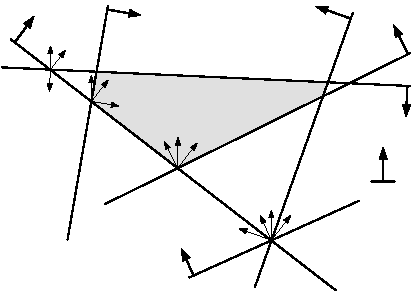
\includegraphics{chapters/chapter_5/figures/Figure2}};
		\node (A) at (-2.9,1.1) {A};
		\node (B) at (-2.2, 0.65) {B};
		\node (C) at (-0.5, -0.65) {C};
		\node (D) at (1.6, -1.6) {D};
		\node (c0) at (3.15, 0) {\footnotesize $c$};
		\node (c1) at (-2.7, 1.8) {\footnotesize $c$};
		\node (c2) at (-2.1, 1.15) {\footnotesize $c$};
		\node (c3) at (-0.5, 0.3) {\footnotesize $c$};
		\node (c4) at (1.1, -0.95) {\footnotesize $c$};
		\node (a11) at (-2.7, 2.2) {\footnotesize $a_1$};
		\node (a12) at (-2.2, 1.7) {\footnotesize $a_1$};
		\node (a13) at (-1.45, 1.1) {\footnotesize $a_1$};
		\node (a14) at (0, 0.1) {\footnotesize $a_1$};
		\node (a15) at (1.5, -1.05) {\footnotesize $a_1$};
		\node (a21) at (-0.9, 2.2) {\footnotesize $a_2$};
		\node (a22) at (-1.3, 0.7) {\footnotesize $a_2$};
		\node (a31) at (3.4, 2.2) {\footnotesize $a_3$};
		\node (a32) at (-0.9, 0.2) {\footnotesize $a_3$};
		\node (a41) at (3.4, 0.4) {\footnotesize $a_4$};
		\node (a42) at (-2.6, 0.8) {\footnotesize $a_4$};
		\node (a51) at (1.7, 2.3) {\footnotesize $a_5$};
		\node (a52) at (0.4, -1.4) {\footnotesize $a_5$};
		\node (a61) at (-0.5, -1.55) {\footnotesize $a_6$};
		\node (a62) at (0.8, -1.05) {\footnotesize $a_6$};
	\end{tikzpicture}
	\caption{$A$ is both primal and dual infeasible; $B$ is primal feasible and dual infeasible; $C$ is primal and dual feasible; $D$ is degenerate.} \label{p1c5:fig:dual_feasibility}
\end{figure}

Notice how in Figure \ref{p1c5:fig:dual_feasibility} neither points A or B are dual feasible, while C represents a dual feasible point, being thus the optimal for the problem depicted. One interesting point to notice is D. Although not feasible, it allows us to see an important effect that degeneracy may cause. Assume for a moment that D is feasible. Then, dual feasibility becomes dependent on the basis representing the vertex. That is,  while the bases $I_B = \braces{1,5}$ and $I_B = \braces{1,6}$ are dual feasible, the basis $I_B = \braces{5,6}$ is not. As we will see, just as it is the case with the simplex method, the dual simplex method, which we will discuss in the next section, might be subject to stalling and cycling from the presence of primal degeneracy, which in turn may also leads to multiple dual feasible (primal optimal) solutions.
 

\section{The dual simplex method}


In general, solution methods in mathematical programming can be either \emph{primal methods}, in which primal feasibility of an initial solution is maintained while seeking for dual feasibility (i.e., primal optimality); or \emph{dual methods}, where dual feasibility is maintained while seeking for primal feasibility (i.e., dual optimality).

As we have seen in Chapter \ref{chapter_4}, the original (or primal) simplex method iterated from an initial basic feasible solution (BFS) until the optimality condition 
%
\begin{equation*}
	\overline{c} = c^\top - c_BB^{-1}A \geq 0
\end{equation*}
%
was observed. Notice that this is precisely the dual feasibility condition $p^\top A \leq c$. 

Being a dual method, the dual version of the simplex method, or the \emph{dual simplex method}, considers conditions in reverse order. That is, it starts from an initial dual feasible solution and iterates in a manner that the primal feasibility condition $B^{-1}b \geq 0$ is \emph{sought} for, while $\overline{c} \geq 0$, or equivalently, $p^\top A \leq c$, is maintained.

To achieve that, one must revise the pivoting of the primal simplex method such that the variable to leave the basis is some $i \in I_B$, with $x_{B(i)} < 0$, while the variable chosen to enter the basis is some $j \in I_N$, such that $\overline{c} \geq 0$ is maintained.

 Consider the $l^\text{th}$ simplex tableau row for which $x_{B(i)} < 0$ of the form $[v_1,\dots, v_n, x_{B(i)}]$; i.e., $v_j$ is the $l^\text{th}$ component of $B^{-1}A_j$.
	 
 For each $j \in I_N$ for which $v_j < 0$, we pick
 %
 \begin{equation*}
 	j' = {\arg\min}_{j \in I_N : v_j < 0} \frac{\overline{c}_j}{|v_j|}.	
 \end{equation*}
 %
 Pivoting is performed by employing elemental row operations to replace $A_{B(i)}$ with $A_j$ in the basis. This implies that $\overline{c}_j \geq 0$ is maintained, since
 %
 \begin{equation*}
	\frac{\overline{c}_j}{|v_j|} \geq \frac{\overline{c}_{j'}}{|v_{j'}|} \Rightarrow \overline{c}_j -|v_j|\frac{\overline{c}_{j'}}{|v_{j'}|} \geq 0 \Rightarrow \overline{c}_j + v_j\frac{\overline{c}_{j'}}{|v_{j'}|} \geq 0, \, \forall j \in J.
 \end{equation*}
%
Notice that it also justifies why we must only consider for entering the basis those variables for which $v_j < 0$. Analogously to the case in the primal simplex method, if we observe that $v_j \ge 0$ for all $j \in J$ , then no limiting condition is imposed in terms the increase in the nonbasic variable (i.e., an unbounded dual, which, according to Corollary \ref{p1c5:cor:weak_duality} (2), implies the original problem is infeasible).

Assuming that the dual is not unbounded, the termination of the dual simplex method is observed when $B^{-1}b \geq 0$ is achieved, and primal-dual optimal solutions have been found, with $x = (x_B,x_N) = (B^{-1}b, 0)$ (i.e., the primal solution) and $p = (p_B, p_N) = (0, c_B^\top B^{-1})$ (dual). Algorithm \ref{p1c5:alg:dual_simplex} presents a pseudocode for the dual simplex method.

\begin{algorithm}[h]
	\caption{Dual simplex method} \label{p1c5:alg:dual_simplex}
	\begin{algorithmic}[1] %line numbering frequency. 
		\State {\bf initialise.} Initial basis $B$ and associated basic solution $x$.
		\While {$x_B = B^{-1}b < 0$ for some component $i \in I_B$} \label{alg:opt_condition} 
			\State Choose some $l$ for which $x_{B(l)} < 0$. Calculate $u = B^{-1}A_j$. 
			\If {$u \geq 0$} \label{alg:unb_condition}
				\State {\bf return} $z = +\infty$.		
			\Else
				\State Form new basis $B = B \setminus \braces{l} \cup \braces{j'}$ where $j' = \arg\min_{j \in I_N : u_j < 0} \frac{\overline{c}_j}{|u_j|}$ 
				\State Calculate $x_B = B^{-1}b$.
			\EndIf
		\EndWhile
		\State {\bf return} optimal basis $B$ and optimal solution $x$.
	\end{algorithmic}
\end{algorithm}

To clarify some of the previous points, let us consider a numerical example. Consider the problem 
%
\begin{align*}
	\mini &x_1 + x_2 \\
	\st &x_1 + 2x_2 \geq 2 \\
	&x_1 \geq  1 \\
	&x_1,x_2 \geq 0.	
\end{align*}	
%
The first thing we must do is convert the greater-or-equal-than inequalities into less-or-equal-than inequalities and add the respective slack variables. This allows us to avoid the inclusion of artificial variables, which are not required anymore since we can allow for primal infeasibility. This leads to the equivalent standard form problem
%
\begin{align*}
	\mini &x_1 + x_2 \\
	\st &-x_1 - 2x_2 + x_3 = -2 \\
	&-x_1 + x_4 = -1 \\
	&x_1,x_2,x_3,x_4 \geq 0.	
\end{align*}

Below is the sequence of tableaus after applying the dual simplex method to solve the problem. The terms in bold font represent the pivot element (i.e., the intersection between the pivot row and pivot column). 

% TODO: Chp5: some pretty editing to make the column width match among tables.

\begin{center}
	\begin{tabular}{c|cccc|c}
		 & $x_1$ & $x_2$ & $x_3$ & $x_4$ & RHS \\ \hline 
		$z$  &  1 & 1 & 0 & 0 & 0  \\ \hline
	   $x_3$ & -1 &\textbf{-2} & 1 & 0 & -2 \\
	   $x_4$ & -1 & 0 & 0 & 1 & -1 \\\hline \hline
	\end{tabular}
	
	\begin{tabular}{c|cccc|c}
		 & $x_1$ & $x_2$ & $x_3$ & $x_4$ & RHS \\ \hline 
		$z$  & 1/2 & 0 & 1/2 & 0 & -1  \\ \hline
	   $x_2$ & 1/2 & 1 & -1/2 & 0 & 1 \\
	   $x_4$ & \textbf{-1} & 0 & 0 & 1 & -1 \\ \hline \hline 
	\end{tabular}
	
	\begin{tabular}{c|cccc|c}
		 & $x_1$ & $x_2$ & $x_3$ & $x_4$ & RHS \\ \hline 
		$z$  & 0 & 0 & 1/2 & 1/2 & -3/2  \\ \hline
	   $x_2$ & 0 & 1 & -1/2 & 1/2 & 1/2 \\
	   $x_1$ & 1 & 0 & 0 & -1 & 1 \\ \hline 
	\end{tabular}
\end{center}

Figure \ref{p1c5:fig:ex1} illustrates the progress of the algorithm both in the primal (Figure \ref{p1c5:fig:ex1_P}) and in the dual (Figure \ref{p1c5:fig:ex1_D}) variable space. Notice how in the primal space the solution remains primal infeasible until a primal feasible solution is reached, that being the optimal for the problem. Also, notice that the coordinates of the dual variables can be extracted from the zeroth row of the simplex tableau.

\begin{figure}[h]
	\centering
	\begin{subfigure}{0.45\textwidth}
		\centering
		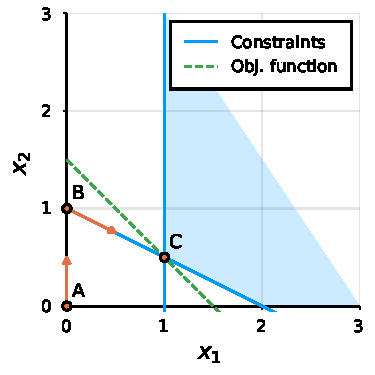
\includegraphics{chapters/chapter_5/figures/primal_plot}
		\caption{The primal-variable space}\label{p1c5:fig:ex1_P}
	\end{subfigure}
	\begin{subfigure}{0.45\textwidth}
		\centering
		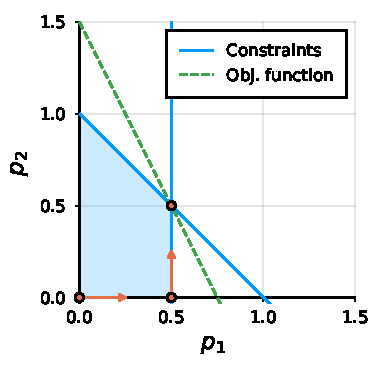
\includegraphics{chapters/chapter_5/figures/dual_plot}
		\caption{The dual-variable space}\label{p1c5:fig:ex1_D}
	\end{subfigure}
	\caption{The progress of the dual simplex method in the primal and dual space.}	\label{p1c5:fig:ex1}
\end{figure}

Some interesting features related to the progress of the dual simplex algorithm are worth highlighting. First, notice that the objective function is monotonically increasing in this case, since $x_{B(l)}\frac{\overline{c}_{j'}}{|v_{j'}|}$ is added to $-c_BB^{-1}b$ and $x_{B(l)} < 0$, meaning that the dual cost increases (recall the convention of having a minus sign so that the zeroth row correctly represent the objective function value, given by the negative of the value displayed in the rightmost column). This illustrates how the solution becomes gradually worse as it compromises optimality in the search for (primal) feasibility. For a nondegenerate problem, this can also be used as an argument for eventual convergence since the dual objective value can only increase and is bounded by the primal optimal value. However, in the presence of dual degeneracy, that is, $\overline{c}_{j} = 0$ for some $j \in I_N$ in the optimal solution, the algorithm can suffer from cycling. As we have seen before, that is an indication that the primal problem has multiple optima. 

The dual simplex method is often the best choice of algorithm, because it typically precludes the need for a Phase I type of method as it is often trivial to find initial dual feasible solutions (the origin, for example, is typically dual feasible in minimisation problems with nonnegative coefficients; similar trivial cases are also well known).

Moreover, dual simplex is the algorithm of choice for resolving a linear programming problem when after finding an optimal solution, you modify the feasible region. Turns out that this procedure is in the core of the methods used to solve integer programming problems, as well as in the Benders decomposition, both topics we will explore later on. The dual simplex method is also more successful than its primal counterpart in combinatorial optimisation problems, which are typically plagued with degeneracy. As we have seen, primal degeneracy simply means multiple dual optima, which are far less problematic under an algorithmic standpoint.

Most professional implementations of the simplex method use by default the dual simplex version. This has several computational reasons, in particular related to more effective Phase I and pricing methods for the dual counterpart.

\vfill
\pagebreak
 
\section{Exercises}

\subsection*{Exercise 5.1: Duality in the transportation problem}
Recall the transportation problem from Chapter 1. Answer the following questions based on the interpretation of the dual price. 


We would like to plan the production and distribution of a certain product, taking into account that the transportation cost is known (e.g., proportional to the distance travelled), the factories (or source nodes) have a supply capacity limit, and the clients (or demand nodes) have known demands. Table \ref{p1c5:tab:E51_transport_problem_data} presents the data related to the problem. 

%
\begin{table}[h]
	\begin{tabular}{r|ccc|c}
    	& & {\it Clients} &\\\hline
    	{\it Factory} & NY & Chicago & Miami & Capacity \\\hline
    	Seattle & 2.5      & 1.7    & 1.8   & 350 \\
    	San Diego & 3.5 & 1.8 & 1.4 & 600 \\\hline
    	Demands & 325 & 300 & 275 & - \\\hline
	\end{tabular}
	\caption{Problem data: unit transportation costs, demands and capacities} \label{p1c5:tab:E51_transport_problem_data}
\end{table}
%
Additionally, we consider that the arcs (routes) from factories to clients have a maximum transportation capacity, assumed to be 250 units for each arc. The problem formulation is then 
%
\begin{align*}
	\mini z = \ &\sum_{i \in I}\sum_{j \in J}c_{ij}x_{ij} \\
	\st & \sum_{j \in J} x_{ij} \leq C_i, ~\forall i \in I \\
	& \sum_{i \in I} x_{ij} \geq D_j, ~\forall j \in J \\
	& x_{ij} \leq A_{ij}, ~\forall i \in I, j \in J \\
	& x_{ij} \geq 0, \forall i \in I, j \in J,
\end{align*}
%
where $C_i$ is the supply capacity of factory $i$, $D_j$ is the demand of client $j$ and $A_{ij}$ is the transportation capacity of the arc between $i$ and $j$.

\begin{itemize}
	\item[(a)] What price would the company be willing to pay for increasing the supply capacity of a given factory?
	\item[(b)] What price would the company be willing to pay for increasing the transportation capacity of a given arc?
\end{itemize}

\subsection*{Exercise 5.2: Dual simplex}
\begin{itemize}
\item[(a)] Solve the problem below by using the dual simplex method. Report both the primal and dual optimal solutions $x$ and $p$ associated with the optimal basis.
\item[(b)] Write the dual formulation of the problem and use strong duality to verify that $x$ and $p$ are optimal.
\end{itemize}
%
\begin{align*}
	\mini & 2x_1 + x_3  \\
	\st & -1/4 x_1 - 1/2 x_2 \leq -3/4 \\
	& 8x_1 + 12 x_2 \leq 20 \\
	& x_1 + 1/2 x_2 - x_3 \leq -1/2 \\
	& 9x_1 + 3 x_2 \geq -6 \\
	& x_1, x_2, x_3 \geq 0.
\end{align*}


\subsection*{Exercise 5.3: Unboundedness and duality}
\noindent Consider the standard-form linear programming problem:
\begin{align*}
	(P) : \mini & c^\top x \\
	\st & Ax = b \\
				& x \ge 0,
\end{align*}
where $A \in \reals^{m \times n}$ and $b \in \reals^m$. Show that if $P$ has a finite optimal solution, then the new problem $\overline{P}$ obtained from $P$ by replacing the right-hand side vector $b$ with another one $\bar{b} \in \reals^m$ cannot be unbounded no matter what value the components of $\bar{b}$ can take.


\subsection*{Exercise 5.4: Dual in matrix form}
\noindent Consider the linear programming problem:
\begin{align*}
	(P) : \mini &  {c^1}^\top x^1 + {c^2}^\top x^2 + {c^3}^\top x^3 & \\
	\text{s.t.} & \\ 
	 & {A}^1{x}^1 + {A}^2{x}^2 + {A}^3{x}^3 \leq b^1 \quad (y^1) \\
	 & {A}^4{x}^1 + {A}^5{x}^2 + {A}^6{x}^3 \leq b^2 \quad (y^2) \\	 
	 & {A}^7{x}^1 + {A}^8{x}^2 + {A}^9{x}^3 \leq b^3 \quad (y^3) \\
	 & x^1 \leq 0 \\
	 & x^2 \geq 0 \\
	 & x^3  \in \reals^{|x^3|},
\end{align*}

\noindent where $A^{1,...,9}$ are matrices, $b^{1,...,3}$, $c^{1,...,3}$ are column vectors, and $y^{1,...,3}$ are the dual variables associated to each constraint. 

\begin{itemize}
	\item[(a)] Write the dual problem in matrix form.
	\item[(b)] Compute the dual optimum for the case in which
	
	$
	A^1 = 
	\begin{bmatrix}
		1 & 2 \\
		3 & 4
	\end{bmatrix}  ; \ 
	A^2 = 
	\begin{bmatrix}
		5 & 1 \\
		0 & 0
	\end{bmatrix}  ; \ 
	A^3 = 
	\begin{bmatrix}
		6 \\
		0
	\end{bmatrix}  ; \ 
	A_4 = 
	\begin{bmatrix}
		1 & 1
	\end{bmatrix}  ; \ 
	A^5 = 
	\begin{bmatrix}
		0 & 1
	\end{bmatrix}  ; \ 
	A^6 = 
	\begin{bmatrix}
		1
	\end{bmatrix}  ; \\ 
	A^7 = 
	\begin{bmatrix}
		0 & 2
	\end{bmatrix}  ; \ 
	A^8 = 
	\begin{bmatrix}
		0 & 0
	\end{bmatrix}  ; \ 
	A^9 = 
	\begin{bmatrix}
		3
	\end{bmatrix}  ; \ 
	c^1 = 
	\begin{bmatrix}
		3 \\
		9
	\end{bmatrix}  ; \ 
	c^2 = 
	\begin{bmatrix}
		4 \\
		2
	\end{bmatrix}  ; \ 
	c^3 = 
	\begin{bmatrix}
		1
	\end{bmatrix}  ; \ 
	b^1 = 
	\begin{bmatrix}
		5 \\
		10
	\end{bmatrix}  ; \\ 
	b^2 = 
	\begin{bmatrix}
		3 
	\end{bmatrix}  ; \ 
	b^3 =
	\begin{bmatrix}
		6
	\end{bmatrix}
	$
	.
		
\end{itemize}


\subsection*{Exercise 5.5: Primal-dual conversion and complementary slackness}
Recall the transportation problem in Exercise 5.1.

\begin{itemize}
\item[(a)] Construct the dual of the problem and solve both the original problem and its dual. 
\item[(b)] Use complementary slackness to verify that the primal and dual solutions are optimal.
\end{itemize}
%





	
	
	\chapter{Linear Programming Duality - Part II} \label{chapter_6}
	
The most direct application of duality in linear programming problems is the interpretation of dual variable values as marginal values associated with constraints, with important economic implications. 

We will also consider the notion of solution stability and restarting the simplex method, once new variables or constraints are added to the problem post optimality. This will have an important consequence for the development of efficient solution methods for integer programming problems, which we will discuss in detail in later chapters.


\section{Sensitivity analysis}

We are interested in analysing aspects associated with the \emph{stability} of the optimal solution $\overline{x}$ in terms of how it changes with the inclusion of new decision variables and constraints or with changes in the input data. Both cases are somewhat motivated by the realisation that problems typically emerge from dynamic settings. Thus, one must assess how \emph{stable} a given plan (represented by $\overline{x}$) is or how it can be adapted in the face of changes in the original problem setting. This kind of analysis is generally referred to as \emph{sensitivity analysis} in the context of linear programming.

First, we will consider the inclusion of new variables or new constraints \emph{after} the optimal solution $\overline{x}$ is obtained. This setting represents, for example, the inclusion of a new product or a new production plant (referring to the context of resource allocation and transportation problems, as discussed in Chapter \ref{chapter_1}) or the consideration of additional constraints imposing new (or previously disregarded) requirements or conditions. The techniques we consider here will also be relevant in the following chapters. We will then discuss specialised methods for large-scale problems and solution techniques for integer programming problems, both topics that heavily rely on the idea of iteratively incrementing linear programming problems with additional constraints (or variables).

The second group of cases relates to changes in the input data. When utilising linear programming models to optimise systems performance, one must bear in mind that there is inherent uncertainty associated with the input data. Be it due to measurement errors or a lack of complete knowledge about the future, one must accept that the input data of these models will, by definition, embed some measure of error. One way of taking this into account is to try to understand the consequences to the optimality of $\overline{x}$ in case of eventual changes in the input data, represented by the matrix $A$, and the vectors $c$ and $b$. We will achieve this by studying the ranges within which variations in these terms do not compromise the optimality of $\overline{x}$. 


\subsection{Adding a new variable} \label{section_611}

Assume that we have solved to optimality the problem $P$ given as
%
\begin{align*}
	P : \mini \, &c^\top x \\
	\st \, & Ax = b \\
	& x \geq 0. 	
\end{align*}

Let us consider that a new variable $x_{n+1}$ with associated column (that is, respective objective function and constraint coefficients) $(c_{n+1}, A_{n+1})$ is added to $P$. This leads to a new augmented problem $P'$ of the form
%
\begin{align*}
	P': \mini \, &c^\top x + c_{n+1}x_{n+1}\\
	\st \, & Ax + A_{n+1}x_{n+1}= b \\
	& x \geq 0, x_{n+1} \geq 0. 	
\end{align*}
%
We need to determine if, after the inclusion of this new variable, the current basis $B$ is still optimal. Making the newly added variable nonbasic yields the basic feasible solution (BFS) $x = (\overline{x}, 0)$. Moreover, we know that the optimality condition $c^\top - c_B^\top B^{-1}b \geq 0$ held before the inclusion of the variable, so we know that all the other reduced costs associated with the nonbasic variables $j \in I_N$ were nonnegative. 

Therefore, the only check that needs to be done is whether the reduced cost associated with $x_{n+1}$ also satisfies the optimality condition, i.e., if
%
\begin{equation*}
	\overline{c}_{n+1} = c_{n+1} - c_B^\top B^{-1}A_{n+1} \geq 0.	
\end{equation*}
%
If the optimality condition is satisfied, the new variable does not change the optimal basis, and the solution $x = (\overline{x}, 0)$ is optimal. Otherwise, one must perform a new simplex iteration, using $B$ as a starting BFS. Notice that in this case, primal feasibility is trivially satisfied, while dual feasibility is not observed (that is, $\overline{c}_{n+1} < 0$). Therefore, primal simplex can be employed, \emph{warm started} by $B$. This is often a far more efficient strategy than resolving $P'$ from scratch.

%TODO: Chp6: Change this to the paint example
Let us consider a numerical example. Consider the problem
%
\begin{align*}
	\mini & -5x_1 -x_2 + 12 x_3 \\
	\st   & 3x_1 + 2x_2 + x_3 = 10 \\
	& 5x_1 + 3x_2 + x_4 = 16 \\
	& x_1, \dots, x_4 \geq 0.
\end{align*}
%
The tableau associated with its optimal solution is given by

\begin{center}
	\begin{tabular}{r|cccc|c} 
	   &$x_1$ & $x_2$ & $x_3$ & $x_4$& RHS \\ \hline	
	   $z$ & 0 & 0 & 2 & 7 & 12\\ \hline
	   $x_1$ & 1 & 0 & -3 & 2 & 2\\
	   $x_2$ & 0 & 1 & 5 & -3 & 2            
	\end{tabular}
\end{center}

Suppose we include a variable $x_5$, for which $c_5 = -1$ and $A_5 = (1,1)$. The modified problem then becomes
%
\begin{align*}
	\mini & -5x_1 -x_2 + 12 x_3 -x_5 	 \\
	\st   & 3x_1 + 2x_2 + x_3 + x_5 = 10 \\
	& 5x_1 + 3x_2 + x_4 + x_5 = 16 \\
	& x_1, \dots, x_5 \geq 0.
\end{align*}
%
We have that the reduced cost of the new variable is given by $\overline{c}_5 = c_5 - c_B^\top B^{-1}A_5 = -4$ and $B^{-1}A_5 = (-1,2)$. The tableau for the optimal basis $B$ considering the new column associated with $x_5$ is thus

\begin{center}
	\begin{tabular}{r|ccccc|c} 
	   &$x_1$ & $x_2$ & $x_3$ & $x_4$& $x_5$ & RHS \\ \hline	
	   $z$ & 0 & 0 & 2 & 7 & -4 & 12   \\ \hline
	   $x_1$ & 1 & 0 & -3 & 2 & -1 & 2 \\
	   $x_2$ & 0 & 1 & 5 & -3 & 2 & 2	            
	\end{tabular}
\end{center}

Notice that this tableau now shows a primal feasible solution that is not optimal and can be further iterated using primal simplex.


\subsection{Adding a new constraint} \label{section_612}

We now focus on the inclusion of additional constraints. Let us assume that a general constraint of the form ${a_{m+1}}^\top x \geq b_{m+1}$ is added to $P$ after it has been solved. We assume it to be an inequality, but notice that $P$ was originally in the standard form.

The first thing to observe is that, if the optimal solution $\overline{x}$ to $P$ satisfy ${a_{m+1}}^\top \overline{x} \geq b_{m+1}$, then nothing changes. Otherwise, we need to rewrite the new constraint accordingly by including a slack variable, obtaining 
%
\begin{equation*}
	{a_{m+1}}^\top x - x_{n+1} = b_{m+1}.
\end{equation*}
%
Notice that doing so changes the matrix $A$ of the original problem $P$, which becomes
%
\begin{equation*}
	\overline{A} = \begin{bmatrix}
				   A & 0 \\ a^\top_{m+1} & -1 
				   \end{bmatrix}.
\end{equation*}

We can reuse the optimal basis $B$ to form a new basis $\overline{B}$ for the problem. This will have the form
%
\begin{equation*}
	\overline{B} = \begin{bmatrix}
		B & 0 \\ a^\top & -1 
	\end{bmatrix},	
\end{equation*}
%
where $a$ are the respective components of $a_{m+1}$ associated with the columns from $A$ that formed $B$. Now, since we have that $\overline{B}^{-1}\overline{B} = I$, we must have that 
%
\begin{equation*}
	\overline{B}^{-1} = \begin{bmatrix}
		B^{-1} & 0 \\ a^\top B^{-1} & -1 
	\end{bmatrix}.	
\end{equation*}
%
Notice however, that the basic solution $(\overline{x}, {a_{m+1}}^\top \overline{x} -  b_{m+1})$ associated with $\overline{B}$ is not feasible, since we assumed that $\overline{x}$ did not satisfy the newly added constraint, i.e., ${a_{m+1}}^\top \overline{x} < b_{m+1}$.

The reduced costs considering the new basis $\overline{B}$ then become
%
\begin{equation*}
	[c^\top ~~ 0] - [c_B^\top ~~ 0]\begin{bmatrix} B^{-1} & 0 \\ a^\top B^{-1} & -1 \end{bmatrix}\begin{bmatrix} A & 0 \\ a_{m+1}^\top & -1 \end{bmatrix} = [c^\top - c^\top_B B^{-1}A ~~ 0].
\end{equation*}
  	
Notice that the new slack variable has a null component as a reduced cost, meaning that it does not violate dual feasibility conditions. Thus, after adding a constraint that makes $\overline{x}$ infeasible, we still have a dual feasible solution that can be immediately used by the dual simplex method, again allowing for warm starting the solution of the new problem.

To build an initial solution in terms of the tableau representation of the simplex method, we must simply add an extra new row, which leads to a new tableau with the following structure
%
\begin{equation*}
	\overline{B}^{-1}A = \begin{bmatrix} B^{-1}A & 0 \\ a^\top B^{-1}A - a_{m+1}^\top & 1 \end{bmatrix}.
\end{equation*}
%		
Let us consider a numerical example again. Consider the same problem as the previous example, but we instead include the additional constraint $x_1 + x_2 \geq 5$, which is violated by the optimal solution $(2,2,0,0)$. In this case, we have that $a_{m+1} = (1,1,0,0)$ and $a^\top B^{-1} A - a^\top_{m+1} = [0, 0, 2, -1]$. This modified problem then looks like
%
%TODO: Chp6: Change this to the paint example
\begin{align*}
	\mini & -5x_1 -x_2 + 12 x_3 \\
	\st   & 3x_1 + 2x_2 + x_3  = 10 \\
	& 5x_1 + 3x_2 + x_4 = 16 \\
	& -x_1 - x_2 + x_5 = -5  \\
	& x_1, \dots, x_5 \geq 0
\end{align*}
%
with associated tableau

\begin{center}
	\begin{tabular}{r|ccccc|c} 
	   &$x_1$ & $x_2$ & $x_3$ & $x_4$ & $x_5$ & RHS \\ \hline	
	   $z$ & 0 & 0 & 2 & 7 & 0 & 12                 \\ \hline
	   $x_1$ & 1 & 0 & -3 & 2 & 0 & 2 				\\
	   $x_2$ & 0 & 1 & 5 & -3 & 0 & 2 				\\
	   $x_5$ &  0 &  0 &  2 & -1 & 1 & -1           
	\end{tabular}
\end{center}

Notice that this tableau indicates that we have a dual feasible solution that is not primal feasible and thus suitable to be solved using dual simplex.
	
A final point to note is that these operations are related to each other in terms of equivalent primal-dual formulations. That is, consider dual of $P$, which is given by
%
\begin{align*}
	D : \maxi   & p^\top b \\
	\st 			& p^\top A \le c.
\end{align*}
%
Then, adding a constraint of the form $p^\top A_{n+1} \leq c_{n+1}$ is equivalent to adding a variable to $P$, exactly as discussed in Section \ref{section_611}.


\subsection{Changing input data} \label{section_613}

We now consider how changes in the input data can influence the optimality of a given basis. Specifically, we consider how to predict whether changes in the vector of independent terms $b$ and objective coefficients $c$ will affect the optimality of the problem. Notice that variations in the coefficient matrix $A$ are left aside.

%TODO: Chp6: include a discussion on variations on the coefficients of A.


\subsubsection{Optimal dual variables as marginal costs}

As before, assume that we have solved $P$ to optimality. As we have seen in Chapter \ref{chapter_4}, the optimal solution $\overline{x}$ with associated basis $B$ satisfies the following optimality conditions: it is a BFS and, therefore (i) $B^{-1}b \geq 0$; and (ii) all reduced costs are nonnegative, i.e., $c^\top - c_B^\top B^{-1}b \geq 0$.

Now, assume that we cause a marginal perturbation on the vector $b$, represented by a vector $d$. That is, assume that we have $B^{-1}(b + d) > 0$, assuming that nondegeneracy is retained.

Recall that the optimality condition $\overline{c} = c^\top - c_B ^\top B^{-1}A \geq 0$ is not influenced by such a marginal perturbation. In other words, for a small change $d$, the optimal basis (i.e., the selection of basic variables) is not disturbed. On the other hand, the optimal value of the basic variables, and consequently, the optimal value, becomes
%
\begin{equation*}
	c_B^\top B^{-1}(b + d) = p^\top(b + d). 
\end{equation*}
%
Notice that $p^\top = c_B^\top B^{-1}$ is optimal for the (respective) dual problem. Thus, a change $d$ causes a change of $p^\top d$ in the optimal value, meaning that the components $p_i$ represent a \emph{marginal value/cost} associated with the independent term $b_i$, for $i \in I$. 

This has important implications in practice, as it allows for \textit{pricing} the values of the resources associated with constraints. For example, suppose the dual value (or price) $p_i$ is associated with a resource whose requirement is given by $b_i$. In that case, any opportunity to remove units of $b_i$ for less than $p_i$ should be seized since it costs $p_i$ to satisfy any additional unit in the requirement $b_i$. A similar interpretation can be made in the context of less-or-equal-than constraints, in which $p_i$ would indicate benefits (or losses, if $p_i > 0$) in increasing the availability of $b_i$. 

For a numerical example, let us consider our paint factory problem once again. 


The following tableau represents the optimal solution
%
\begin{center}
	\begin{tabular}{c|cccccc|c}
		     & $x_1$ & $x_2$ & $x_3$ & $x_4$ & $x_5$ & $x_6$ & RHS \\ \hline 
		$z$  & 0  & 0 & 3/4 & 1/2 & 0 & 0 & 21   \\ \hline
	   $x_1$ & 1  & 0 & 1/4 & -1/2 & 0 & 0 & 3 \\
	   $x_2$ & 0  & 1 &-1/8 & 3/4 & 0 & 0 & 3/2  \\
	   $x_5$ & 0  & 0 & 3/8 &-5/4 & 1 & 0 & 5/2  \\
	   $x_6$ & 0  & 0 & 1/8 &-3/4 & 0 & 1 & 1/2  \\ \hline
	\end{tabular}
\end{center}
%
where $x_3$ and $x_4$ were the slack variables associated with raw material M1 and M2, respectively. In this case, we have that 
$$
B^{-1} = \begin{bmatrix}
 		   1/4 & -1/2 & 0 & 0 \\
		  -1/8 & 3/4 & 0 & 0 \\
		   3/8 &-5/4 & 1 & 0 \\
		   1/8 &-3/4 & 0 & 1
 		 \end{bmatrix} \text{ and } p = c_B^\top B^{-1} =  
 		 \begin{bmatrix}
 		 	-5 \\
 		 	-4 \\
 		 	0 \\
 		 	0
 		 \end{bmatrix}^\top
 		 \begin{bmatrix}
 		   1/4 & -1/2 & 0 & 0 \\
		  -1/8 & 3/4 & 0 & 0 \\
		   3/8 &-5/4 & 1 & 0 \\
		   1/8 &-3/4 & 0 & 1
 		 \end{bmatrix}  = 
 		 \begin{bmatrix}
 		 	-3/4 \\ -1/2 \\ 0 \\ 0
 		 \end{bmatrix}
$$
Notice that these are values of the entries in the $z$-row below the slack variables $x_3, \dots, x_6$, except the minus sign. This is because the $z$-rows contain the entries for $c - p^\top B^{-1}$ and we have an objective function coefficient of zero for all slack variables, i.e., $c_j = 0$, for $j = 3,\dots,6$. Also, recall that the paint factory problem is a maximisation problem, so $p$ represents the decrease in the objective function value. In this, we see that removing one unit of M1 would decrease the objective function by 3/4 and removing one unit of M2 would similarly decrease the objective value by 1/2. Analogous, increasing M1 or M2 availability by one unit would increase the objective function value by 3/4 and 1/2, respectively. 


\subsubsection{Changes in the vector $b$}

Suppose that some component $b_i$ changes and becomes $b_i + \delta$, with $\delta \in \reals$. We are interested in the range for $\delta$ within which the basis $B$ remains optimal.

First, we must notice that optimality conditions $\overline{c} = c^\top - c^\top_B B^{-1}A \geq 0$ are not directly affected by variation in the vector $b$. This means that the choice of variable indices $j \in I_B$ to form the basis $B$ will, in principle, be \emph{stable} unless the change in $b_i$ is such that $B$ is rendered \emph{infeasible}. Thus, we need to study the conditions in which  feasibility is retained, or, more specifically, if (recall the $e_i$ is the vector of zeros except for the $i\nth$ component being 1)
%
\begin{equation*}
	B^{-1}(b + \delta e_i) \geq 0.	
\end{equation*}

Let $g = (g_{1i}, \dots, g_{mi})$ be the $i\nth$ column of $B^{-1}$. Thus
%
\begin{equation*}
	B^{-1}(b + \delta e_i) \geq 0 \Rightarrow x_B + \delta g \geq 0 \Rightarrow x_{B(j)} + \delta g_{ji} \geq 0, \ j = 1,\dots, m.  
\end{equation*}
%
Notice that this is equivalent to having $\delta$ within the range
%
\begin{equation*}
	\max_{j : g_{ji} > 0}\left(-\frac{x_{B(j)}}{g_{ji}}\right) \leq \delta \leq \min_{j : g_{ji} < 0}\left(-\frac{x_{B(j)}}{g_{ji}}\right).	
\end{equation*}

In other words, changing $b_i$ will incur changes in the value of the basic variables, and thus, we must determine the range within which all basic variables remain nonnegative (i.e., feasible).

Let us consider a numerical example. Once again, consider the problem from Section \ref{section_611}. The optimal tableau was given by
%TODO: Chp6: Change this to the paint example

\begin{center}
	\begin{tabular}{c|cccc|c} 
	   &$x_1$ & $x_2$ & $x_3$ & $x_4$& RHS \\ \hline	
	   $z$ & 0 & 0 & 2 & 7 & 12\\
	   $x_1$ & 1 & 0 & -3 & 2 & 2\\
	   $x_2$ & 0 & 1 & 5 & -3 & 2\\	            
	\end{tabular}	
\end{center}

Suppose that $b_1$ will change by $\delta$ in the constraint $3x_1 + 2x_2 + x_3  = 10$. Notice that the first column of $B^{-1}$ can be directly extracted from the optimal tableau and is given by $(-3,5)$. The optimal basis will remain feasible if $2 - 3\delta \geq 0$ and $2 + 5\delta \geq 0$, and thus $-2/5 \leq \delta \leq 2/3$.

Notice that this means that we can calculate the change in the objective function value as a function of $\delta \in [-2/5, 2/3]$. Within this range, the optimal cost changes as 
%
\begin{equation*}
	c_B^\top (b + \delta e_i) = p^\top b + \delta p_i,	
\end{equation*}
%
where $p^\top = c_B ^\top B^{-1}$ is the optimal dual solution. In case the variation falls outside that range, this means that some of the basic variables will become negative. However, since the dual feasibility conditions are not affected by changes in $b_i$, one can still reutilise the basis $B$ using dual simplex to find a new optimal solution.


\subsubsection{Changes in the vector $c$}

We now consider the case where variations are expected in the objective function coefficients. Suppose that some component $c_j$ becomes $c_j + \delta$. In this case, optimality conditions become a concern. Two scenarios can occur. First, it might be that the changing coefficient is associated with a variable $j \in J$ that happens to be nonbasic ($j \in I_N$) in the optimal solution. In this case, we have that optimality will be retained as long as the nonbasic variable remains ``not attractive'', i.e., the reduced cost associated with $j$ remains nonnegative. More precisely put, the basis $B$ will remain optimal if
%
\begin{equation*}
	(c_j + \delta) - c_BB^{-1}A_j \geq 0 \Rightarrow \delta \geq -\overline{c}_j.
\end{equation*}
%

The second scenario concerns changes in variables that are basic in the optimal solution, i.e., $j \in I_B$. In that case, the optimality conditions are directly affected, meaning that we have to analyse the range of variation for $\delta$ within which the optimality conditions are maintained, i.e., the reduced costs remain nonnegative.

Let $c_j$ is the coefficient of the $l^{\text{th}}$ basic variable, that is $j = B(l)$. In this case, $c_B$ becomes $c_B + \delta e_l$, meaning that all optimality conditions are simultaneously affected. Thus, we have to define a range for $\delta$ in which the condition
%
\begin{equation*}
	(c_B + \delta e_l)^\top B^{-1}A_i \leq c_i, \, \forall i \neq j 
\end{equation*}
%
holds. Notice that we do not need to consider $j$ since $x_j$ is a basic variable, and thus, its reduced costs are assumed to remain zero.

Considering the tableau representation, we can use the $l^{\text{th}}$ row and examine the conditions for which $\delta q_{li} \leq \overline{c}_i, \forall i \neq j$, where $q_{li}$ is the $i^{\text{th}}$ entry in the $l^{\text{th}}$ row of $B^{-1}A_i$.

Let us once again consider the previous example, with optimal tableau 

\begin{center}
	\begin{tabular}{c|cccc|c} 
	   &$x_1$ & $x_2$ & $x_3$ & $x_4$& RHS \\ \hline	
	   $z$ & 0 & 0 & 2 & 7 & 12\\
	   $x_1$ & 1 & 0 & -3 & 2 & 2\\
	   $x_2$ & 0 & 1 & 5 & -3 & 2\\	            
	\end{tabular}	
\end{center}

First, let us consider variations in the objective function coefficients of variables $x_3$ and $x_4$. Since both variables are nonbasic in the optimal basis, the allowed variation for them is given by
%
\begin{equation*}
	\delta_3 \geq -\overline{c}_3 = -2 \text{ and } 
    \delta_4 \geq -\overline{c}_4 = -7. 	
\end{equation*}
%
Two points to notice. First, notice that both intervals are one-sided. This means that one should only be concerned with variations that decrease the reduced cost value since increases in their value can never cause any changes in the optimality conditions. Second, notice that the allowed variation is trivially the negative value of the reduced cost. For variations that turn the reduced costs negative, the current basis can be utilised as a starting point for the primal simplex.

Now, let us consider a variation in the basic variable $x_1$. Notice that in this case, we have to analyse the impact in all reduced costs, except for $x_1$ itself. Using the tableau, we have that $q_l = [1, 0, -3, 2]$ and thus
%
\begin{align*}
	& \delta_1 q_{12} \leq \overline{c}_2 \Rightarrow 0 \leq 0 \\
	& \delta_1 q_{13} \leq \overline{c}_3 \Rightarrow \delta_1 \geq -2/3  \\
	& \delta_1 q_{14} \leq \overline{c}_4 \Rightarrow \delta_1 \leq 7/2, 
\end{align*}
%
implying that $-2/3 \leq \delta_1 \leq 7/2$. Like before, for a change outside this range, primal simplex can be readily employed.


\section{Cones and extreme rays}

We now change the course of our discussion towards some results that will be useful in identifying two non-ordinary situations when employing the simplex method: unboundedness and infeasibility. Typically, these are consequences of issues related to the data and/or with modelling assumptions and are challenging in that they prevent us from obtaining a solution from the model. As we will see, infeasibility and unboundedness can be identified using duality and are all connected by the notion of cones, which we formally give in Definition \ref{p1c6:def:cone}.

\begin{definition}[Cones]\label{p1c6:def:cone}
	A set $C \subset \reals^n$ is a cone if $\lambda x \in C$ for all $\lambda \geq 0$ and all $x \in C$.	
\end{definition}

A cone $C$ can be understood as a set formed by the nonnegative scaling of a collection of vectors $x \in C$. Notice that it implies that $ 0 \in C$. Often, it will be the case that $ 0 \in C$ is an extreme point of $C$ and in that case, we say that $C$ is \emph{pointed}. As one might suspect, in the context of linear programming, we will be mostly interested in a specific type of cone, those known are \emph{polyhedral cones}. Polyhedral cones are sets of the form 
%
\begin{equation*}
	P = \braces{x \in \reals^n : Ax \geq 0}.
\end{equation*}
%
Figure \ref{p1c6:fig:poly_cone} illustrates a polyhedral cone in $\reals^3$ formed by the intersection of three half-spaces. 
%
\begin{figure}[h]
	\begin{tikzpicture}
		\node (pic) at (0,0) {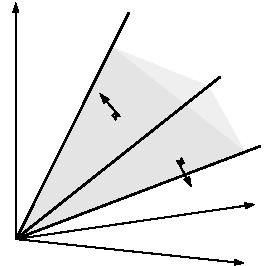
\includegraphics{chapters/chapter_6/figures/Figure1.pdf}};
		\node (x1) at (2,-2) {$x_1$};
		\node (x2) at (2,-1) {$x_2$};
		\node[right] (x3) at (-2,2) {$x_3$};
		\node (a1) at (-0.3,0.8) {$a_1$};
		\node (a2) at (1.1,-0.4) {$a_2$};
	\end{tikzpicture}
	\caption{A polyhedral cone in $\reals^3$ formed by 3 half-spaces. The third (with normal vector $a_3$ perpendicular to the page plan) cannot be seen} \label{p1c6:fig:poly_cone}
\end{figure}
%

Some interesting properties can be immediately concluded regarding polyhedral cones. First, they are convex sets, since they are polyhedral sets (cf. Theorem \ref{p1c2:thm:convexity}). Also, the origin is an extreme point, and thus, polyhedral cones are always pointed. Furthermore, just like general polyhedral sets, a cone $C \in \reals^n$ will always be associated with a collection of $n$ linearly independent vectors. Corollary \ref{p1c6:cor:polyhedral_cones} summarises these points. Notice we pose it as a corollary because these are immediate consequences of Theorem \ref{p1c3:thm:exist_extreme_point}. 

\begin{corollary}\label{p1c6:cor:polyhedral_cones} 
	Let $C \subset \reals^n$ be a polyhedral cone defined by constraints $\braces{a_i^\top x \geq 0}_{i =1,\dots,m}$. Then the following are equivalent
	\begin{enumerate}
		\item $0$ is an extreme point of $C$;
		\item $C$ does not contain a line;
		\item There exists $n$ vectors in $a_1, \dots, a_m$ that are LI.	
	\end{enumerate}
\end{corollary}

\begin{proof}
	The proof of Theorem \ref{p1c3:thm:exist_extreme_point} verbatim, with $P = C$.	
\end{proof}

Notice that $0 \in C$ is the unique extreme point of the polyhedral cone $C$. To see that, let $0 \neq x \in C$, $x_1 = (1/2) x$ and $x_2 = (3/2)x$. Note that $x_1, x_2 \in C$, and $x \neq x_1 \neq x_2$. Setting $\lambda_1 = \lambda_2 = 1/2$, we have that $\lambda_1x_1  + \lambda_2x_2 = x$ and thus, $x$ is not an extreme point (cf. Definition \ref{p1c2:def:extreme_point}). 


\subsection{Recession cones and extreme rays} \label{section_621}

We now focus on a specific type of cone, called \emph{recession cones}. In the context of linear optimisation, recession cones are useful for identifying directions of unboundedness. Let us first formally define the concept.

\begin{definition}[Recession cone] \label{c1_p6:def:recession_cone}
	Consider the polyhedral set $P = \braces{x \in \reals^n : Ax \geq b}$. The recession cone at $\overline{x} \in P$, denoted ${\bf recc}(P)$, is defined as
	\begin{equation*}
		{\bf recc}(P) = \braces{d \in \reals^n : A(\overline{x} + \lambda d) \geq b, \lambda \geq 0} \text{ or } \braces{d \in \reals^n : Ad \geq 0}. 	
	\end{equation*}
\end{definition}

Notice that the definition states that a recession cone comprises all directions $d$ along which one can move from $\overline{x} \in P$ without ever leaving $P$. However, notice that the definition does not depend on $\overline{x}$, meaning that the recession cone is unique for the polyhedral set $P$, regardless of its ``origin''. Furthermore, notice that Definition \ref{c1_p6:def:recession_cone} implies that recession cones of polyhedral sets are polyhedral cones. 

We say that any directions $d \in {\bf recc}(P)$ is a \emph{ray}. Thus, bounded polyhedra can be alternatively defined as polyhedral sets that do not contain rays. 

\begin{figure}[h]
	\begin{tikzpicture}
		\node (pic) at (0,0) {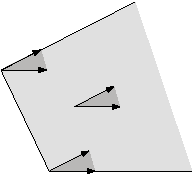
\includegraphics{chapters/chapter_6/figures/Figure2.pdf}};
	\end{tikzpicture}
	\caption{Representation of the recession cone of a polyhedral set} \label{p1c6:fig:recession_cone}	
\end{figure}

Figure \ref{p1c6:fig:recession_cone} illustrates the concept of recession cones. Notice that the cone is purposely placed in several places to illustrate the independence of the point $\overline{x} \in P$.

Finally, the recession cone for a standard form polyhedral set $P = \braces{x \in \reals^n : Ax = b, x \geq 0}$ is given by 
%
\begin{equation*}
	{\bf recc}(P) = \braces{d \in \reals^n : Ad = 0, d \geq 0}.	
\end{equation*} 


\subsection{Unbounded problems}

To identify unboundedness in linear programming problems, we must check for the existence of \emph{extreme rays}. Extreme rays are analogous to extreme points, but defined with a ``loose'' degree of freedom. Definition \ref{p1c6:def:extreme_ray} provides a technical definition of extreme rays.

\begin{definition}[Extreme ray] \label{p1c6:def:extreme_ray}
	Let $C \subset \reals^n$ be a nonempty polyhedral cone. A nonzero $x \in C$ is an extreme ray if there are $n-1$ linearly independent active constraints at $x$.
\end{definition} 

Notice that we are interested in extreme rays of the recession cone ${\bf recc} (P)$ of the polyhedral set $P$. However, it is typical to say that they are extreme rays of $P$. Figure \ref{p1c6:fig:extreme_rays} illustrates the concept of extreme rays in polyhedral cones.

\begin{figure}[h]
	\begin{tikzpicture}
		\node (pic) at (0,0) {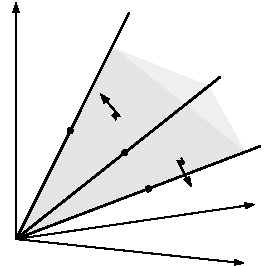
\includegraphics{chapters/chapter_6/figures/Figure3.pdf}};
		\node (x1) at (2,-2) {$x_1$};
		\node (x2) at (2,-1) {$x_2$};
		\node[right] (x3) at (-2,2) {$x_3$};
		\node (a1) at (-0.3,0.8) {$a_1$};
		\node (a2) at (1.1,-0.4) {$a_2$};
		\node[left] (d1) at (-1,0.1) {$d_1$};
		\node(d2) at (-0.4,-0.2) {$d_2$};
		\node(d3) at (0,-0.75) {$d_3$};								
	\end{tikzpicture}
	\caption{A polyhedral cone formed by the intersection of three half-spaces (the normal vector $a_3$ is perpendicular to the plane of the picture and cannot be seen). Directions $d_1$, $d_2$, and $d_3$ represent extreme rays.} \label{p1c6:fig:extreme_rays}	
\end{figure}

Notice that, just like extreme points, the number of extreme rays is finite by definition. In fact, we say that two extreme rays are equivalent if they are positive multiples corresponding to the same $n-1$ linearly independent active constraints.


The existence of extreme rays can be used to verify unboundedness in linear programming problems. The mere existence of extreme rays does not suffice since unboundedness is a consequence of the extreme ray being a direction of improvement for the objective function. To demonstrate this, let us first describe unboundedness in polyhedral cones, which we can then use to show the unboundedness in polyhedral sets.

\begin{theorem}[Unboundedness in polyhedral cones]\label{p1c6:thm:unb_cones}
	Let $P : \mini\braces{c^\top x : x \in C}$, with \linebreak $C = \braces{a_i^\top x \geq 0, i \in [m]}$. The optimal value is equal to $-\infty$ if and only if some extreme ray $d \in C$ satisfies $c^\top d < 0$.
\end{theorem}

\begin{proof}
	If $c^\top d < 0$, then $P$ is unbounded, since $c^\top x \rightarrow -\infty$ along $d$. Also, there exists some $x \in C$ for which $c^\top x < 0$ can be scaled to -1.
	
	Let $P = \braces{x \in \reals^n : a_i^\top x \geq 0, i =1,\dots,m , c^\top x = -1}$. Since $0 \in C$, $P$ has at least one extreme point $\braces{a_i}_{i=1}^m$ and thus span $\reals^n$ (cf. Theorem \ref{p1c3:thm:exist_extreme_point}). Let $d$ be one of those. As we have $n$ linearly-independent active constraints at $d$, $n-1$ of the constraints $\braces{a_i^\top x \geq 0}_{i =1}^m$ must be active (plus $c^\top x = -1$), and thus $d$ is an extreme ray.
\end{proof}

We can now expand the result to general polyhedral sets.

\begin{theorem}[Unboundedness in polyhedral sets]\label{p1c6:thm:unb_polyhedra} 
	Let $P : \mini\braces{c^\top x : x \in X}$ with $X = \braces{x \in \reals^n : Ax \geq b}$ and assume that the feasible set has at least one extreme point. Then, the optimal value is $-\infty$ if and only if $c^\top d < 0$.  	
\end{theorem}

\begin{proof}
	As before, if $c^\top d < 0$, then $P$ is unbounded, since $c^\top x \rightarrow -\infty$ along $d$. Now, let 
	$D : \maxi \braces{p^\top b : p^\top A = c^\top, p \ge 0}$ be the dual of $P$. Recall that, if $P$ is unbounded, then $D$ is infeasible, and so must be $D^0 : \maxi \braces{p^\top 0 : p^\top A = c^\top, p \ge 0}$. This implies that the primal $P^0 : \mini \braces{c^\top x : Ax \geq 0}$ is unbounded (as 0 is feasible).
			
	The existence of at least one extreme point for $P$ implies that the rows $\braces{a_i}_{i=1,\dots,m}$ of $A$ span $\reals^n$ and  ${\bf recc}(X) \hspace{-3pt} =  \hspace{-3pt}\braces{x \in \reals^n : Ax \geq 0}$ is pointed. Thus, by Theorem \ref{p1c6:thm:unb_cones} there exists $d$ such that $c^\top d < 0$. \qedhere
\end{proof}

We now focus on how this can be utilised in the context of the simplex method. It turns out that once unboundedness is identified in the simplex method, one can extract the extreme ray causing the said unboundedness. In fact, most professional-grade solvers are capable of returning extreme (or unbounded) rays, which is helpful in the process of understanding the causes for unboundedness in the model. We will also see in the next chapter that these extreme rays are also used in the context of specialised solution methods.

To see that is possible, let $P : \mini\braces{c^\top x : x \in X}$ with $X = \braces{x \in \reals^n : Ax = b, x \geq 0}$ and assume that, for a given basis $B$, we conclude that the optimal value is $-\infty$, that is, the problem is unbounded. In the context of the simplex method, this implies that we found a nonbasic variable $x_j$ for which the reduced cost $\overline{c}_j < 0$ and the $j^\text{th}$ column of $B^{-1}A_j$ has no positive coefficient. Nevertheless, we can still form the feasible direction $d= [d_B ~ d_N]$ as before, with
%
\begin{equation*}
	d_B = -B^{-1}A_j \text{ and } 
	d_N = \begin{cases}
 		d_j = 1 \\
 		d_i = 0, \forall i \in I_N \setminus \braces{j}.
 	\end{cases}
\end{equation*}
%
This direction $d$ is precisely an extreme ray for $P$. To see that, first, notice that $Ad = 0$ and $d \geq 0$, thus	$d \in {\bf recc}(X)$. Moreover, there are $n-1$ active constraints at $d$: $m$ in $Ad = 0$ and $n-m-1$ in $d_i = 0$ for $i \in I_N \setminus \braces{j}$. The last thing to notice is that $\overline{c}_j = c^\top d < 0$, which shows the unboundedness in the direction $d$. 

 

\subsection{Farkas' lemma}

We now focus on the idea of generating certificates of infeasibility for linear programming problems. That is, we show that if a problem $P$ is infeasible, then there is a structure that can be identified to certify the infeasibility. To see how this works, consider the two polyhedral sets
%
\begin{align*}
	&X = \braces{x \in \reals^n : Ax = b,  x \geq 0} \text{ and } \\ 
	&Y = \braces{p \in \reals^m : p^\top A x \geq 0, p^\top b < 0}.
\end{align*}
%
If there exists any $p \in Y$, then there is no $x \in X$ for which $p^\top Ax = p^\top b$ (and in turn $Ax = b$) holds. Thus, $X$ must be empty. Notice that this can be used to infer that a problem $P$ with a feasibility set represented by $X$ prior to solving $P$ itself, by means of solving the \emph{feasibility problem} of finding a vector $p \in Y$. 

We now pose this relationship more formally via a result generally known as the Farkas' lemma.

\begin{theorem}[Farkas' lemma] \label{p1c6:thm:farkas}
	Let $A$ be a $m \times n$ matrix and $b \in \reals^m$. Then, exactly one of the following statements hold
	\begin{enumerate}
		\item[(1)] There exists some $x \geq 0$ such that $Ax = b$;
		\item[(2)] there exists some vector $p$ such that $p^\top A \geq 0$, $p^\top b < 0$. 
	\end{enumerate}
\end{theorem}

\begin{proof}
	Assume that (1) is satisfied. If $p^\top A \geq 0$, then $p^\top b =$ $p^\top Ax \geq 0$, which violates (2).
	
	Now, consider the primal-dual pair $P : \mini\braces{0^\top x : Ax = b, x \geq 0}$ and $D : \maxi\hspace{-2pt}\braces{p^\top b : p^\top A \geq 0}$. Being $P$ infeasible, $D$ must be unbounded (instead of infeasible) since $p = 0$ is feasible for $D$. Thus, $p^\top b < 0$ for some $p \neq 0$. 	
\end{proof}

The Farkas' lemma has a nice geometrical interpretation that represents the mutually exclusive relationship between the two sets. For that, notice that we can think of $b$ as being a conic combination of the columns $A_j$ of $A$, for some $x \ge 0$. If that cannot be the case, then there exists a hyperplane that separates $b$ and the cone formed by the columns of $A$, $C=\braces{y \in \reals^m : y = Ax}$. This is illustrated in Figure \ref{p1c6:fig:farkas}. Notice that the separation caused by such a hyperplane with normal vector $p$ implies that $p^\top Ax \geq 0$ and $p^\top b < 0$, i.e., $Ax$ and $b$ are on the opposite sides of the hyperplane. 

\begin{figure}[H]
	\begin{tikzpicture}
		\node (pic) at (0,0) {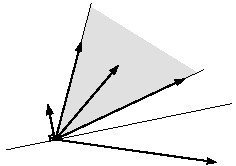
\includegraphics{chapters/chapter_6/figures/Figure4.pdf}};
		\node (A1) at (-1,0.6) {$A_1$};
		\node (A2) at (0,0.5) {$A_2$};
		\node (A3) at (1,0.4) {$A_3$};
		\node (b) at (1.6,-1) {$b$};
		\node (p) at (-1.3, -0.2) {$p$};
	\end{tikzpicture}	
	\caption{Since $b \not\in X$, $p^\top x=0$ separates them} \label{p1c6:fig:farkas}	
\end{figure}

\vfill


\pagebreak	

\section{Exercises}

\subsection*{Exercise 6.1: Sensitivity analysis in the RHS}
Consider the following linear programming problem and its optimal tableau below:

\begin{align*}
	\mini & -2x_1 - x_2 + x_3 \\
	\st   & x_1 + 2x_2 + x_3 \le 8 \\
		  & -x_1 + x_2 - 2x_3 \le 4 \\
		  & 3x_1 + x_2 \le 10 \\
		  & x_1, x_2, x_3 \ge 0.	 
\end{align*}

\begin{center}
	\begin{tabular}{c|cccccc|c}
		        & $x_1$ & $x_2$ & $x_3$ & $x_4$ & $x_5$ & $x_6$ & RHS \\
		\hline
		    $z$ &   0   &   0   &   1.2 &   0.2 &   0   &   0.6 & -7.6 \\
		\hline
		  $x_1$ &   1   &   0   &  -0.2 &  -0.2 &   0   &   0.4 &  2.4  \\
		  $x_2$ &   0   &   1   &   0.6 &   0.6 &   0   &  -0.2 &  2.8  \\
		  $x_5$ &   0   &   0   &  -2.8 &  -0.8 &   1   &   0.6 &  3.6  \\
	\end{tabular}	
\end{center}


\begin{itemize}
	\item [(a)] If you were to choose between increasing in 1 unit the right-hand side of any constraints, which one would you choose, and why? What is the effect of the increase on the optimal cost?
	\item [(b)] Perform a sensitivity analysis on the model to discover what is the range of alteration in the RHS in which the same effect calculated in item (a) can be expected. \emph{HINT}: JuMP (from version 0.21.6) includes the function ``lp\_sensitivity\_report()'' that you can use to help performing the analysis.
\end{itemize}


\subsection*{Exercise 6.2: Extreme points and extreme rays}

\begin{itemize}
	\item[(a)] Let $P=\{(x_1,x_2) : x_1 - x_2 = 0,~ x_1 + x_2 = 0\}$. What are the extreme points and the extreme rays of $P$?
	\item[(b)] Let $P=\{(x_1,x_2) : 4x_1 + 2x_2 \geq 0,~ 2x_1 + x_2 \leq 1\}$. What are the extreme points and the extreme rays of $P$?
	\item[(c)] For the polyhedron of part (b), is it possible to express each one of its elements as a convex combination of its extreme points plus a nonnegative linear combination of its extreme rays? Is this compatible with the Resolution Theorem? 
\end{itemize}

\subsection*{Exercise 6.3: From Farkas' lemma to duality}
Use the Farkas' lemma to prove the duality theorem for a linear programming problem involving constraints of the form $a'_ix = b_i, a'_ix \geq b_i$, and nonegativity constraints for some of the variables $x_j$. \emph{Hint}: Start by deriving the form of the set of feasible directions at an optimal solution.


\subsection*{Exercise 6.4: Adding a constraint}
Consider the linear programming problem below with optimal basis $[x_1, x_2, x_5, x_6]$ and dual variables $p_1, \dots, p_4$.

\begin{align*}
	\maxi & 2x_1 + x_2 \\
	\st   & 2x_1 + 2x_2 \le 9 \quad (p_1) \\
	      & 2x_1 - x_2 \le 3 \quad (p_2) \\
	      & x_1 \le 3 \quad (p_3) \\
	      & x_2 \le 4 \quad (p_4) \\
	      & x_1, x_2 \ge 0.
\end{align*}

\begin{itemize}
	\item[(a)] Find the primal and dual optimal solutions. \emph{HINT}: You can use complementary slackness, once having the primal optimum, to find the dual optimal solution.
	\item[(b)] Suppose we add a new constraint $6x_1 - x_2 \leq 6$, classify the primal and dual former optimal points stating if they: (i) remain optimal; (ii) remain feasible but not optimal; or (iii) become infeasible.
	\item[(c)] Consider the new problem from item (b) and find the new dual optimal point through one dual simplex iteration. After that, find the primal optimum.
\end{itemize}








	
	\chapter{Barrier Method for Linear Programming} \label{chapter_7}
	\section{Barrier methods} \label{section_71}

In this chapter, we look into barrier methods as an alternative for solving linear programming problems. Barrier methods stem from early developments of methods for solving constrained nonlinear programming problems which were mainly characterised by the \emph{strict} satisfaction of the constraints throughout the method. Because of this feature, these methods became generally known as interior point methods. This is however not the case anymore, and most implementations of interior point methods benefit from features that allow the search to ``leave the interior'' of the feasible region. Hence, it became common to refer to these methods with the more general name of barrier methods.

A subclass of barrier methods called \emph{primal-dual methods} distinguishes itself as an efficient method, with practical performance surpassing in many cases that of the simplex method. Currently, most professional-grade solvers have built-in implementations of barrier methods.

In essence, barrier methods are the method of choice of many nonlinear \emph{local solvers}, which are targeted towards nonlinear optimisation problems. The term local refers to the fact that solutions found can only be guaranteed to be locally optimal. Of course, for convex optimisation problems, this is not an issue, as a local solution is globally optimal.

In general, the simplex methods often perform better in small and medium problems, whilst barrier methods typically perform better on large-scale problems. This is largely because, as we will see, the main operation in a barrier method is solving (large) linear systems of equations, which can be done rather efficiently and in ways that exploit the structure of the problem (e.g., matrix sparsity can be exploited by factorisation techniques) to reap computational performance improvements.


\section{Newton's method with equality constraints} 


In essence, barrier methods employ a variant of Newton's method to solve the optimality conditions of optimisation problems. In the context of linear programming problems, this is equivalent to finding solutions that are both primal and dual feasible\footnote{Recall that the satisfaction of complementarity conditions in the linear case is a consequence of primal and dual feasibility, cf. Theorem \ref{p1c2:thm:complemetarity_slackness}.}.

We consider a version of Newton's method called the Newton-Raphson (NR) method, which was originally conceived for finding roots of vector functions. Let $f: \reals^n \to \reals^n$, with $f_i : \reals^n \to \reals$ differentiable for $i = 1,\dots,n$.

We wish to find a solution $x^*$ that is a root for $f$, i.e., $f(x^*) = 0$. For that, we must solve the system of equations given by
	$$ 
	f(x) = \begin{bmatrix} f_1(x) \\ \vdots \\ f_n(x) \end{bmatrix} = \begin{bmatrix} 0 \\ \vdots \\ 0 \end{bmatrix}.
	$$
	
The NR method starts from an initial guess $x^k$ for $x^*$ and iterates by finding the root for a \emph{linear} (i.e., first-order Taylor) approximation of $f$ at $x^k$. Under suitable conditions, including having a starting point $x^0$ that is within a neighbourhood of the root of $f$, the sequence $\braces{x^k}_{k\to\infty}$ converges to $x^*$.

Let us clearly state how the method iterates. At a given $x^k$, the first-order approximation of $f(x)$ is given by
	$$ 
	f(x^k + d) = f(x^k) + \nabla f(x^k)^\top d,
	$$
	where $\nabla f(x^k)$ is the \emph{Jacobian} of $f(x)$, which is defined as
	$$ 
	\nabla f(x^k) = \begin{bmatrix} \nabla f_1(x^k)^\top \\ \vdots \\ \nabla f_n(x^k)^\top \end{bmatrix}. 
	$$
	
The algorithm proceeds by finding the step to be taken from $x^k$ to reach the root of the first-order approximation of $f$ at $x^k$. This means that we want to obtain a Newton direction $d$ such that it solves the first-order approximation of $f(x^k + d) = 0$. Thus, we must solve
	%
	\begin{equation*}
		f(x^k) + \nabla f(x^k)^\top d = 0 \Rightarrow
		d = -\nabla f(x^k)^{-1}f(x^k).
	\end{equation*}
	
%TODO Chp7: expand on this and explain the role of \epsilon in the process. It ends rather abruptly.	
	
Consider the following numerical example. Suppose we would like to find the root of $f$ with $x^0 = (1,0,1)$, where $f$ is given by 
	$$
	f(x) = \begin{bmatrix}f_1(x) \\ f_2(x) \\ f_3(x) \end{bmatrix} = \begin{bmatrix} x_1^2 + x_2^2 + x_3^2 -3 \\ x_1^2 + x_2^2 - x_3 - 1 \\ x_1 + x_2 + x_3 - 3 \end{bmatrix}
	$$
	The Jacobian of $f$ is given by 
	$$
	\nabla f(x)=\begin{bmatrix} 2x_1 & 2x_2 & 2x_3 \\ 2x_1 & 2x_2 & -1 \\ 1 & 1 & 1\end{bmatrix}.
	$$
	
	The algorithm starts by calculating $d^0$, which is given by
	$$
	d^0 = -[\nabla f(x^0)]^{-1}f(x^0) = - \begin{bmatrix} 2 & 0 & 2 \\ 2 & 0 & -1 \\ 1 & 1 & 1\end{bmatrix}^{-1}\begin{bmatrix} -1 \\ -1 \\ -1 \end{bmatrix} = \begin{bmatrix} 1/2 \\ 1/2 \\ 0 \end{bmatrix}.
	$$ 
	%
	Thus, the first point is 
	$$
	x^1 = x^0 + d^0 = \begin{bmatrix} 3/2 & 1/2 & 1\end{bmatrix}.
	$$ 
	%
	To infer that the method has converged, we can either check whether $f(x^k) \approx 0$ or whether $||x^{k+1} - x^{k}||_2 = || d^{k} ||_2 \approx 0$. As $||x^1 - x^0||_2 = || d^0 ||_2 \approx 0.7$, and $f(x^1) = \brackets{1/2, 1/2, 0}$, the point $x^1$ is not a root, and the method carries on until we find that $|| d^k|| < \epsilon$. If we adopt a numerical tolerance of $\epsilon = 0.01$, meaning that any number below this threshold is deemed acceptably close to zero, then $x^* = (1, 1, 1)$ is reached after approximately 20 iterations.	

\section{Interior point methods linear programming problems}
	
We start by focusing on the primal-dual interior point method, as originally proposed. Then, we will focus on the modifications that make it capable of iterating through some not necessarily interior solutions in a strict sense. 	

We start by considering our linear programming problem in standard form 
	\begin{align*}
		(P) :~ \mini \ &c^\top x \\
		\st &Ax = b,  \\
		&x \ge 0, 
	\end{align*}
	%
	and its associated dual, which is stated as
	%
	\begin{align*}
		(D) :~ \maxi \ &b^\top p \\
		\st &A^\top p + u = c, \\
		&u \ge 0. 
	\end{align*}
	%
	Notice that the dual is also posed in a form where the inequalities (originally $A^\top p \le c$) are converted to equalities requiring the additional variable $u$. An alternative way to think about $u$ is as if it were the dual variable associated with the nonnegativity constraints $x \ge 0$. 
	
Recall that the optimality conditions for problem $P$ can be expressed as
	%
	\begin{align} 
		& Ax = b, \ \ x \ge 0, \label{p1c7:eq:optimality_conditions_primal} \\
		& A^\top p + u = c, \ \ u \ge 0, \label{p1c7:eq:optimality_conditions_dual} \\
		& u^\top x = 0. \label{p1c7:eq:optimality_conditions_cc}  
	\end{align}
	%
	The first two conditions are primal \eqref{p1c7:eq:optimality_conditions_primal} and dual \eqref{p1c7:eq:optimality_conditions_dual} feasibility conditions, while \eqref{p1c7:eq:optimality_conditions_cc} is an alternative way of stating complementarity conditions on the nonnegativity constraints $x \ge 0$.
	
One initial idea could be simply, from a purely methodological standpoint, to employ NR to solve the above system of equations. The caveat, however, is that one must observe and retain the nonnegativity conditions $x > 0$ and $u >0$, which are an important complicating factor in this setting. Indeed, departing from a feasible solution $(x,p,u)$, one could employ NR to find a solution for \eqref{p1c7:eq:optimality_conditions_primal}-\eqref{p1c7:eq:optimality_conditions_cc} while controlling the steps taken in each Newton direction such that the nonnegativity conditions $x > 0$ and $u >0$ are retained, in a similar fashion to how it is done in the simplex method. However, it turns out that Newton directions obtained from successive iterations of \eqref{p1c7:eq:optimality_conditions_primal}- \eqref{p1c7:eq:optimality_conditions_cc} typically require the steps to be considerably small so that the nonnegativity conditions are retained, which renders the algorithm less useful from a practical standpoint.
	   
	
This is precisely when the notion of an interior solution plays a role. An \emph{interior point} is defined as a point that satisfies primal and dual feasibility conditions strictly, that is $Ax = b$ with $x > 0$, and $A^\top p + u = c$ with $u >0$, implying that the complementarity conditions \eqref{p1c7:eq:optimality_conditions_cc} are \emph{violated}. This notion of interior points is useful in that it allows for the definition of less ``aggressive'' Newton directions, which aim towards directions that reduce the amount of violation in the complementarity conditions. Thus, we can alternatively consider the system with \emph{relaxed} complementarity conditions in which we define the scalar $\mu > 0$ and restate the optimality conditions as 	
	%
	\begin{align*}
		& Ax = b, \ \ x \geq 0,\\ 
		& A^\top p + u = c, \ \ u \geq 0, \\
		& u_j x_j = \mu, \ \forall j \in J. 
	\end{align*}
	%
	Then, we use these relaxed optimality conditions to obtain Newton directions, while, simultaneously, gradually making $\mu \to 0$. By doing so, one can obtain not only directions that can be explored with larger step sizes, thus making more progress per iteration, but also yield methods with better numerical properties.
	
To see how that can be made operational, let us first define some helpful notation. Let $X\in \reals^{n\times n}$ and $U \in \reals^{n \times n}$ be defined as
	%
	$$
	X = \diag(x) = \begin{bmatrix} \ddots & & \\   
	                                        & x_i & \\
	                                        & & \ddots     
	                 \end{bmatrix}
	                 \text{ and }
	U = \diag(u) = \begin{bmatrix} \ddots & & \\   
	                                        & u_i & \\
	                                        & & \ddots     
	                 \end{bmatrix}               
	$$
	%
	and let $e = [1,\dots,1]^\top$ be a vector of ones of suitable dimension. We can rewrite the optimality conditions \eqref{p1c7:eq:optimality_conditions_primal}- \eqref{p1c7:eq:optimality_conditions_cc} in matrix form as 
	%
	\begin{align*}
		&Ax = b, \ x > 0, \\ 
		&A^\top p + u = c, \ u > 0,\\ 
		&XUe = 0, 
	\end{align*}
	%
 	and, analogously, state their relaxed version (i.e., with relaxed complementarity conditions) as
 	%
 	\begin{align}
		&Ax = b, \ x > 0, \label{p1c7:eq:optimality_conditions_matrix_primal}\\ 
		&A^\top p + u = c, \ u > 0, \label{p1c7:eq:optimality_conditions_matrix_dual}\\ 
		&XUe = \mu e. \label{p1c7:eq:optimality_conditions_matrix_relaxed_cc}
	\end{align}

We start from a feasible solution $(x^{k}, p^{k}, u^{k})$. We can then employ NR to solve the system \eqref{p1c7:eq:optimality_conditions_matrix_primal}-\eqref{p1c7:eq:optimality_conditions_matrix_relaxed_cc} for a given value of $\mu$. That amounts to finding the Newton direction $d$ that solves $f(x^k) + \nabla f(x^k)^\top d = 0$, in which
	%
	\begin{equation*}
	f(x^k) = \begin{bmatrix}
				Ax^k - b \\
				A^\top p^k + u^k - c \\
				X^k U^k e - \mu e 
			   \end{bmatrix},	   
		\ \nabla f(x^k) = \begin{bmatrix}
					   A & 0 & 0 \\
					   0 & A^\top & I \\
					   U^k & 0 & X^k	
					  \end{bmatrix}
		 \text{ and } d = (d_x^k, d_p^k, d_u^k) = 
			\begin{bmatrix}
			x - x^k \\ 
			p - p^k \\
			u - u^k
		\end{bmatrix}.
	\end{equation*}	
	
Once the direction $d^k = (d_x^k, d_p^k, d_u^k)$ is obtained, we must calculate step sizes that can be taken in the direction $d^k$ that also retain feasibility conditions, meaning that they do not violate $x >0$ and $u > 0$ at the new point. One simple idea is to follow the same procedure as the simplex method. That is, let $\theta_p^k$ and $\theta_d^k$ be the iteration $k$ step sizes for $x$ and $(p,u)$, respectively. Then they can be set as
	%
	\begin{equation*}
		\theta_p^k = \min_{i:d_{x_i}^k < 0} - \frac{x_i^k}{d_{x_i}^k} \text{ and }	\theta_d^k = \min_{i:d_{u_i}^k < 0} - \frac{u_i^k}{d_{u_i}^k},
	\end{equation*}
		%
		where $d_{x_i}^k$ and $d_{u_i}^k$ are the $i$-th component of the vectors $d_x^k$ and $d_u^k$, respectively, and $i = 1, \dots, n$. In practice, there are alternative, and arguably more efficient, ways to set step sizes, but they all are such that their maximum sizes are $\theta_p$ and $\theta_d$ as above and always strictly smaller than one (notice that our constraints are such that $x$ and $u$ are strictly positive).
		
		Once we calculated appropriate step sizes, we can then make 
		$$
		(x^{k+1}, p^{k+1}, u^{k+1}) = (x^{k} + \theta_{p}^kd_x^k, p^{k} + \theta_d^k d_p^{k}, u^{k} + \theta_d^k d_u^k).
	$$
	Then, we proceed by updating $\mu$ as $\mu = \beta \mu$, with $\beta \in (0,1)$ and repeat the same procedure until convergence, i.e., until $\mu$ is sufficiently small.  
		
Before discussing in more detail the practicalities of the method, let us take an alternative perspective on showing how the notion of interior plays a role in the design of the algorithm, which requires us to consider the notion of barrier functions. This will also serve as a justification for the name ``barrier methods''. 
	
	
\section{Barrier methods for linear programming problems}


Barrier methods are a class of optimisation methods designed to handle inequality-constrained problems of the form
	%
	\begin{align*}
	(P) : \mini \ & f(x) \\
	\st & g_i(x) \leq 0, \ i = 1,\dots,m \\
	& Ax = b. 
	\end{align*}
	%
	These methods use the notion of \emph{barrier functions} to remove inequality constraints and have them represented implicitly as an objective function term. This allows for the use of NR as the underpinning numerical method of a solution algorithm. 
	
To see how the method works, we can think of a barrier function as a surrogate for a \emph{feasibility indicator function} $I$ that reacts to infeasibility in $g_i(x) \leq 0$, $\forall i \in  \braces{1,\dots, m}$\footnote{The technical name of this function is the \emph{characteristic function}, which is arguably a less informative name.}. That is, $I : \reals \to \reals$ is such that
	%
	\begin{equation*}
	I(y) = \begin{cases} 0, &\text{if } y \leq 0 \\
	                     \infty, &\text{if } y > 0.  
	       \end{cases}
	\end{equation*} 

With that definition for $I$ at hand, we can then reformulate our problem as	
	%
	\begin{align*}
		\mini \ & f(x) + \sum_{i=1}^m I(g_i(x)) \\
		\st &Ax = b. 
	\end{align*}
	
The issue however is that $I$ is not numerically favourable, due to its nature of ``shooting to infinity'' (including the discontinuity it creates) whenever a solution $x$ is infeasible to the original problem. To circumvent that, we can use barrier functions instead, which are chosen to mimic the behaviour of $I$, whilst retaining more favourable numerical properties. The most widespread choice for barrier functions is the logarithmic barrier, which is given by
	%
	\begin{equation*}
		B_\mu(y) = -\mu \ln(-y)
	\end{equation*}
	%
	where $\mu > 0$ sets the accuracy of the barrier term $B_\mu(y)$. Figure \ref{p1c7:fig:barrier_function} illustrates the influence of $\mu$ in the shape of the barrier function for the unidimensional case. Notice how, as $\mu$ decreases, the logarithmic barrier more closely resembles the indicator function $I$.
	
\begin{figure}
	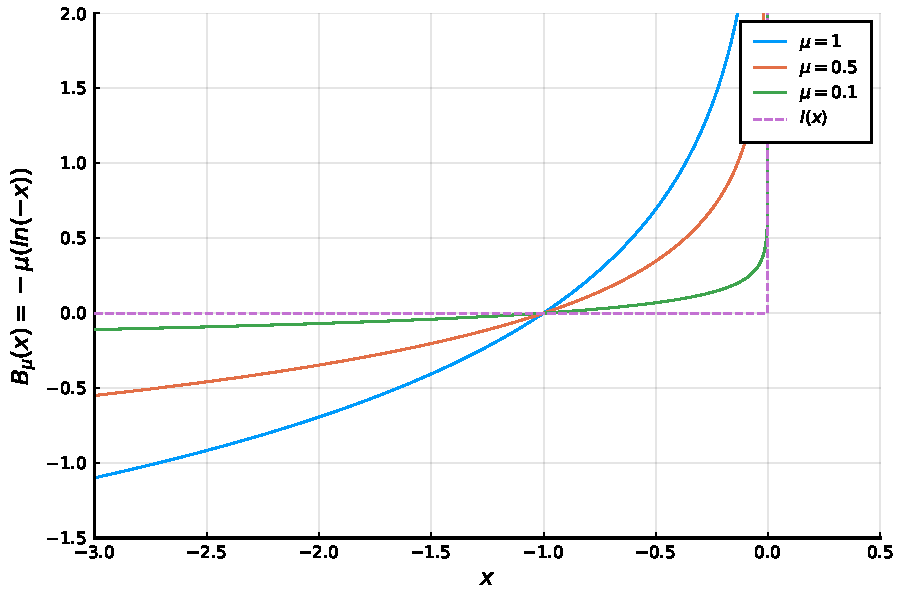
\includegraphics[width=0.8\textwidth]{chapters/chapter_7/figures/different_mu.pdf}
	\caption{Alternative barrier functions for different values of $\mu$. The dashed line represents the indicator function $I(x)$ going to infinity when $x > 0$} \label{p1c7:fig:barrier_function}
\end{figure}

Using $B_\mu$ as the barrier function, the \emph{barrier problem} $P_\mu$ can be formulated as
	%
	\begin{align*}
		(P_\mu) : \mini \ &f(x) - \mu \sum_{i=1}^m\ln(-g_i(x)) \\
		\st & Ax = b.
	\end{align*}
	%
	This formulation has a number of important benefits. First, notice how this problem is such that, if one were to apply NR to solve its optimality conditions, one would be faced with solving linear systems of equations, regardless of the nature of the constraints $g_i(x) \le 0$, $i = 1,\dots, m$ (recall that NR solves first-order approximations of the original system of equations). This creates a bridge between linear algebra techniques and a wide range of nonlinear optimisation problems. 
	
Moreover, as discussed earlier, one can also gradually decrease $\mu$ by making $\mu^{k+1} = \beta\mu$ with $\beta \in (0,1)$. This method is an idea generally known as Sequential Unconstrained Minimisation Technique (SUMT). As one may suspect, as $\mu \rightarrow 0$, we have that $x^*(\mu) \rightarrow x^*$, where $x^*(\mu)$ and $x^*$ are the optimal values for problems $P_\mu$ and $P$, respectively. However, for small values of $\mu$, the barrier problem becomes challenging numerically, which does not come as a surprise as the barrier resembles more and more the indicator function $I$ and all its associated numerical issues. 

Let us illustrate the above with an example. Consider the nonlinear problem 
	$$
	P : \mini \braces{f(x) = (x + 1)^2 : x \geq 0}.
	$$ 
	Notice that the unconstrained optimum would be $x =-1$ but the constrained optimum is $x^* = 0$. For this example, the barrier problem $P_\mu$ is
	%
	$$P_\mu : \mini f(x) + B_\mu(x) = (x + 1)^2 - \mu \ln(x).$$
	%
	Because this is a univariate convex function, we know that the optimum is attained where the derivative $(f(x) + B_\mu(x))' = 0$. Thus, we have that
	%
	\begin{align*}
		& f^{~\prime}(x) + B_\mu^\prime(x) = 0 \\
		& 2(x+1) - \frac{\mu}{x} = 2x^2 + 2x -\mu = 0.
	\end{align*}
	%
	The positive solution (since we must have that $x > 0$) of $2x^2 + 2x -\mu = 0$ is given by
	$$ x^*(\mu) = \frac{-2 + \sqrt{4 + 8\mu}}{4}.  
	$$ 
	Notice that $\lim_{\mu \rightarrow 0}x^*(\mu) = 0$, which is indeed the optimal $x^*$ for $P$. Figure \ref{p1c7:fig:example-barrier} plots the function $f(x) + B_\mu(x)$ for alternative values of $\mu$ indicating their minima (found by substituting the value of $\mu$ in the expression for $x^*(\mu)$). 

\begin{figure}
	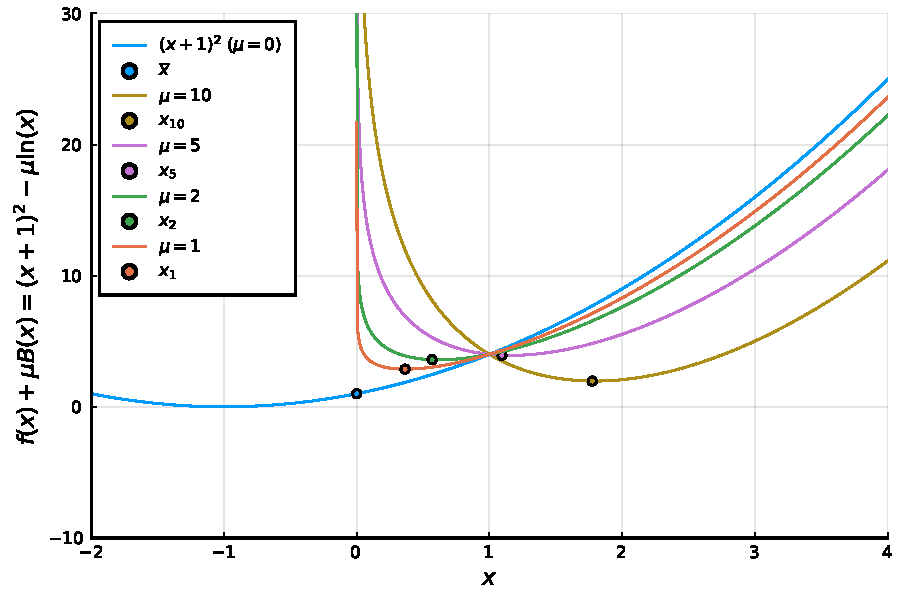
\includegraphics[width=0.8\textwidth]{chapters/chapter_7/figures/ex-barrier.pdf}
	\caption{The optimal values of $P_\mu$ for different values of $\mu$. Notice the trajectory formed by the points $x^*(\mu)$ as $\mu \to 0$.} \label{p1c7:fig:example-barrier} 	
\end{figure}


\subsubsection{The notion of interiority}

There is an interesting link between barrier methods and the notion of interior points, which is, in a way, the reason why the two ideas are equivalent. Before we show they are indeed equivalent, let us explore this notion of interiority.

For a large enough $\mu$, the solution of the barrier problem $P_\mu$ is close to the \emph{analytic centre} of the polyhedral feasibility set. The analytic centre of a polyhedral set is	the point at which the distance to all of the hyperplanes forming the set is maximal. More precisely, consider the polyhedral set $S = \braces{x \in \reals^n : Ax \leq b} $. The analytic centre of $S$ is given by the optimal solution $x^*$ of the following problem
	%
	\begin{align*}
		\maxi_x & \prod_{i=1}^m (b_i - a_i ^\top x) \\
		\st & x \in S. 	
	\end{align*}
	%	 
	Notice that we obtain an equivalent problem, that is, a problem would return the same optimal solution $x^*$, if we take the logarithm of the objective function, this would lead to
	%
	\begin{align*}
		\mini_x & \sum_{i=1}^m -\ln(b_i - a_i ^\top x) \\
		\st & x \in S. 	
	\end{align*}
	%
	This allows us to infer something about the behaviour of the barrier method. For larger values of $\mu$, the optimal solution of $x^*(\mu)$ will lie close to the analytical centre of the feasible region. On the other hand, as $\mu$ diminishes, the ``pull'' towards the centre slowly decays whilst the pull caused by the objective function (that is, by its gradient $-\nabla f(x)$) slowly becomes more prevalent and steers the solution towards $x^*$.


\section{Barrier methods for linear programming problems}

Let us consider again our linear programming problem in standard form 
	$$
	(P) : \mini\braces{c^\top x : Ax = b, x \ge 0}
	$$ 
	to which we want to devise a barrier problem. The barrier problem for $P$ is
	%
	\begin{align*}
		(P_\mu) :~ \mini \ &c^\top x  - \mu\sum_{i=1}^n \ln(x_j)\\
		\st &Ax = b \ \ ( \text{and} \ \ x > 0). 
	\end{align*}
	
By looking at this formulation, and relating to the previous discussion, a barrier method for a linear programming problem operates such that in earlier iterations, or for larger $\mu$ values, the optimal solution $x(\mu)^*$ of $P_\mu$ tends to be pushed towards the centre of the feasible region, where $x >0$. As $\mu \to 0$, the influence of $c^\top x$ gradually takes over, steering the solution towards the optimal $x^*$ of $P$. 

 The most remarkable result, which ties together interior point methods and barrier methods for linear programming problems, is the following. If we derive the Karush-Kuhn-Tucker optimality conditions (Section \ref{p2c7:sec:KKT} in the nonlinear optimization section of these notes) for $P_\mu$, we obtain the following set of conditions
	% 
	\begin{align*}
		&Ax = b, \ x > 0\\ 
		&A^\top p = c - \mu\left(\frac{1}{x_1},\dots,\frac{1}{x_n}\right).
	\end{align*}
	% 
	Using the same notation as before (i.e., defining $X$ and $U$), these can be equivalently rewritten as 
		\begin{align*}
			&Ax = b, \ x > 0 \\ 
			&A^\top p + u = c \\ 
			&u = \mu X^{-1}e ~\Rightarrow~ XUe = \mu e, 
		\end{align*}
	which are exactly \eqref{p1c7:eq:optimality_conditions_matrix_primal}-\eqref{p1c7:eq:optimality_conditions_matrix_relaxed_cc}. Thus, it becomes clear that relaxing the complementarity conditions in the way that we have done before is equivalent to imposing logarithmic barriers to the nonnegativity constraints of $x$. 
	
There are many important consequences for the analysis of the method once this link is established. One immediate consequence relates to the convergence of the method, meaning that as primal and dual feasibility conditions are satisfied throughout the iterations of the method, as $\mu \to 0$, complementarity conditions are satisfied in the limit, thus converging to the solution of the original linear problem $P$. 

Indeed, the trajectory formed by successive solutions $\braces{(x(\mu_k), p(\mu_k), u(\mu_k))}_{k=1,2,\dots}$ is called the \emph{central path}, which is a consequence of the interiority forced by the barrier function. This property is the reason why barrier methods are sometimes called ``path-following'' methods.

It is interesting to also notice the information encoded in \eqref{p1c7:eq:optimality_conditions_matrix_relaxed_cc}. First, notice from \eqref{p1c7:eq:optimality_conditions_matrix_dual} that 
	%
	\begin{align*}
		& A^\top p + u = c \Leftrightarrow \\	
		& p^\top (A x) + u^\top x = c^\top x  \Leftrightarrow  \\
		& u^\top x = c^\top x - p^\top b.
	\end{align*}
	%
	That is, $u^\top x$ provides us with an estimate of the current \emph{duality gap}, which can be used to estimate how far we are from the optimal solution. Moreover, notice that
	$$
	u^\top x = \sum_{i =1}^n u(\mu)_i x(\mu)_i = n\mu 
	$$
	%
	meaning that the term $\mu$ indicates the average amount of violation per $x$ and $u$ variable pairs at $(x^k, p^k, u^k)$. 


\subsubsection{A practical implementation of the barrier method}

The version of the barrier method most often used has a few additional ideas incorporated into the algorithm. One of the main ideas is using a \emph{single Newton step} for each value of $\mu$. That effectively means that the iterates do not delineate exactly the central path formed by successively smaller values of $\mu$, but rather follow it only approximately. 

More precisely, assume we start with $\mu_k > 0$ and a $(x^k, p^k, u^k)$ close to $(x(\mu_k), p(\mu_k), u(\mu_k))$. Then, for a small $\beta \in (0,1)$, a Newton step with $\mu_{k+1} = \beta \mu_k$ leads to $(x^{k+1}, p^{k+1}, u^{k+1})$ close to $x(\mu_{k+1}), p(\mu_{k+1}), u(\mu_{k+1})$. Now, to be more precise in terms of what is meant by close, we must refer to the notion of \emph{central paths neighbourhoods}.

A common neighbourhood often used in convergence analysis of the barrier method is
	%
	\begin{equation*}
		N_{\mu_k}(\alpha) =  \braces{(x, p, u) : \|X  U e - \mu_k e \|_2 \leq \alpha \mu_k},
	\end{equation*} 
	%
	which essentially consists of a bound on the difference between the expected value of the complementarity condition violation $\mu$ and that observed by the current solution $(x^k, p^k, u^k)$. The parameter $\alpha \in (0,1]$ is an arbitrary scalar that dictates the amount of such difference tolerated and effectively controls how wide the neighbourhood is. Then, by setting values for $\beta$ and $\alpha$ that satisfy $\beta = 1 - \frac{\sigma}{\sqrt{n}}$ for some $\sigma \in (0,1)$ (e.g., $\alpha = \sigma = 0.1)$, one can guarantee that the complementarity violation of the next iteration to be bounded such that $(x^{k+1}, p^{k+1}, u^{k+1}) \in N_{\mu_{k+1}}(\alpha)$ \cite{gondzio2012interior}. Figure \ref{p1c7:fig:central-path-and-neighbourhoods} illustrate this idea, depicting two successive iterates of the method remaining within the shrinking neighbourhoods $N_{\mu_k}(\alpha)$. 
	
	\begin{figure}
			\begin{tikzpicture}
				\node at (0,0) {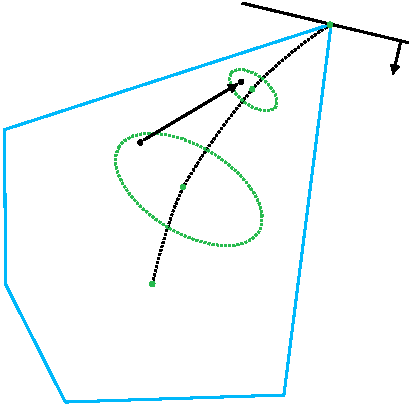
\includegraphics{chapters/chapter_7/figures/central_path_lp-eps-converted-to.pdf}};
		%		\draw[help lines] (-4,-4) grid (4,4);
				\node[below] at (-0.4,-1.2) {$x_{+\infty}$};
				\node[right] at (-0.4,0.2) {$x_{\mu_k}$};		
				\node[below] at (1.3,2.1) {$x_{\mu_{k+1}}$};
				\node[right] at (-1.2,0.9) {$x^k$};
				\node[above] at (0.8,2.05) {$x^{k+1}$};
				\node[below] at (3.5,2.6) {$c$};
				\node[below] at (0.4,-0.6) {$N_{\mu_1}(\alpha)$};
				\node[below] at (1.1,1.7) {$N_{\mu_2}(\alpha)$};	
			\end{tikzpicture}	
			\caption{An illustrative representation of the central path and how the method follows it approximately}
			\label{p1c7:fig:central-path-and-neighbourhoods} 
	\end{figure}
	
Another important aspect of the method relates to the feasibility requirements of each step. Current implementations of the method can be shown to converge under particular conditions even if the feasibility requirements are eased in the Newton system. In this case, it needs to be shown that the Newton direction is also such that the amount of infeasibility in the system decreases as the algorithm progresses. 
	
The infeasible version of the algorithm is such that the so-called perturbed (or relaxed) system
	%
	\begin{equation*} 	
		\begin{bmatrix} A  & 0 & 0 \\ 
						0  & A^\top & I \\ 
						U^k  & 0 & X^k 
		\end{bmatrix} 
		\begin{bmatrix} d_x^{k+1} \\ 
					    d_p^{k+1} \\ 
					    d_u^{k+1} 
		\end{bmatrix} =  
		\begin{bmatrix} 0 \\ 
						0 \\ 
						\mu_{k+1} e - X^k U^k e 
		\end{bmatrix} 
	\end{equation*} 
	%
	becomes 
	%
	\begin{equation}\label{p1c7:eq:infeasible_perturbed_system}
	\begin{bmatrix} A  & 0 & 0 \\ 
					0  & A^\top & I \\ 
					U^k & 0 & X^k 
	\end{bmatrix} 
	\begin{bmatrix}d_x^{k+1} \\ 
				   d_p^{k+1} \\ 
				   d_u^{k+1} 
	\end{bmatrix} = - 
	\begin{bmatrix} Ax^k - b \\ A^\top p^k + u^k - c \\ X^k U^ke -\mu_{k+1}e \end{bmatrix}, 
	\end{equation}
	where $\mu_{k+1} = \beta\mu_k$.

The primal residual $r_p(x) = Ax - b$ and dual residual $r_d(p,u) = A^\top p + u - c$ allow the method to iterate through solutions $(x^k, p^k, u^k)$ that do not satisfy primal and/ or dual feasibility. A caveat though is that the convergence analysis of this variant is more involved and requires additional assumptions on the parameterisation of the algorithm for convergence. 

To see how the residuals decay at each iteration, notice the following. Let $r(w) = r(x,p,u) = (r_p(x), r_d(p,u))$. The optimality conditions \eqref{p1c7:eq:optimality_conditions_primal}-\eqref{p1c7:eq:optimality_conditions_cc} require the residuals to vanish, that is, $r(w) = 0$. Now, let us consider the first-order approximation for $r$ at $w^k$ for a Newton step $d_w$. This amounts to the following:
	$$
	r(w^k + d_w) \approx r(w^k) + Dr(w^k)d_w,
	$$
	where $Dr(w^k)$ is the Jacobian of $r$ evaluated at $w^k$. One can notice that, in this notation, the solution $d_w^{k+1}$ to \eqref{p1c7:eq:infeasible_perturbed_system} is such that 
		$$
		Dr(w^k) d_w^{k+1} = -r(w^k).
		$$

Now, let us consider the directional derivative of the norm of the updated residues in the direction $d_w^{k+1}$. That leads to the following conclusion
	%
	\begin{equation*}
		\frac{d}{dt} \big\| r(w^k + td_w^{k+1}) \big\|_2^2 \Big|_{t = 0} = 2r(w^k)^\top Dr(w^k)d_w^{k+1} = -2 \| r(w^k) \|_2^2 < 0.
	\end{equation*}
	%
	This shows that the direction $d_w^{k+1}$ is a descent direction for the norm of the residues at $w^k$ which leads to their eventual vanishing.	
	
We are finally ready to pose the pseudocode of a working version of the barrier method, which is displayed in Algorithm \ref{p1c7:alg:barrier_method}.
	%
	\captionsetup[algorithm]{font=footnotesize}
	\begin{algorithm}[H]
	\caption{Barrier method for LP} \label{p1c7:alg:barrier_method}
	\begin{algorithmic}[1] 
	\State {\bf initialise.} \text{(primal-dual feasible)} $(x^0, p^0, u^0)$, $\epsilon > 0$, $\mu_0 = \mu_1>0$, $\beta \in (0,1)$, $k = 0$. 
	\While {$n \mu_k > \epsilon$}
	    \State compute $d^{k+1} = (d_x^{k+1}, d_p^{k+1}, d_u^{k+1})$ using \eqref{p1c7:eq:infeasible_perturbed_system} 
	    \State compute appropriate step size $\theta^{k+1} = (\theta_p^{k+1}, \theta_d^{k+1}$)
	    \State $(x^{k+1}, p^{k+1}, u^{k+1}) = (x^k, p^k, u^k) + \theta^{k+1}d^{k+1}$
	    \State $k = k+1$
	    \State $\mu_{k+1} = \beta\mu_k$
	\EndWhile
	\State {\bf return} $(x^k, p^k, u^k)$.
	\end{algorithmic} 
	\end{algorithm}
	
Some final remarks are worth making. Barrier methods are perhaps the only class of methods that are known for being strong contenders to the dominance of simplex method-based approaches for linear programming problems. This stems from both a theoretical and an experimental perspective. The convergence analysis available in \cite{gondzio2012interior} shows that the number of iterations of the barrier method, for suitable parameterisation, is $O(\sqrt{n}\ln(1/\epsilon))$, whilst, for the simplex method, a similar analysis would bound the number of iterations to be of the order $O(2^n)$. A conclusion stemming from these results would be that barrier methods, being polynomial complexity algorithms, should outperform the simplex method.

But in practice, this is not necessarily the case. Despite its complexity analysis, the simplex method in practice often requires $O(m)$ iterations (i.e., a typically modest multiple of $m$), where $m$ is the number of columns in the basis. On the other hand, practical observation has shown barrier methods to typically require $\sqrt{n}$ iterations or less and appear to be somewhat insensitive to growth in the number of variables further to a certain point. On the other hand, one iteration of the simplex method is rather inexpensive from a computational standpoint, while one iteration of a barrier method is a potentially computationally demanding operation (as it requires the solution of a large linear system of equations).

In general, simplex-method-based solvers are faster on problems of small to medium dimensions, while barrier methods are competitive, and often faster, on large problems. However, this is not a rule, as the performance is dependent on the structure of the particular application. In the end, it all boils down to how effectively the underlying liner system solver can exploit particular structural features that allow using dedicated numerical algebra methods (e.g., sparsity and the use of Cholesky decomposition combined with triangular solves).

Moreover, barrier methods are generally not able to take full advantage of any prior knowledge about the solution, such as an estimate of the solution itself or some suboptimal basis. Hence, barrier methods are less useful than simplex approaches in situations in which ``warm-start'' information is available. One situation of this type involves branch-and-bound algorithms for solving integer programs, where each node in the branch-and-bound tree requires the solution of a linear program that differs only slightly from one already solved in the parent node. In other situations, we may wish to solve a sequence of linear programs in which the data is perturbed slightly to investigate the sensitivity of the solutions, or in which we approximate a non-linear optimisation problem by a sequence of linear programs. In none of the aforementioned scenarios can barrier methods be used as efficiently as the simplex method (dual or primal, depending on the context).

\vfill
\pagebreak	

\section{Exercises}


\subsection*{Exercise 7.1: Step size rule for the barrier method}
Solve the following optimisation problem using the barrier method.


\begin{align}
 (P) \quad &   \min \quad  x_1 + x_2\\
    &\text{s.t. } \ \quad 2x_1 + x_2 \geq 8 \\
    & \quad\quad\quad x_1 + 2x_2 \geq 10 \\
    & \quad\quad\quad x_i \geq 0, \ \forall i \in \{1,2\}
\end{align}

\begin{itemize}
    \item[(a)] Solve the problem using a constant step size $\theta = 1$.
    \item[(b)] Derive a step size rule for the barrier method based on retaining primal and dual feasibility.
    \item[(c)] Amend the solution from part (a) to incorporate the step size calculation stage. Utilise the step size rule derived in part (b). Then, resolve the problem.
\end{itemize}



	
	\chapter{Integer Programming Models} \label{chapter_8}
	\section{Types of integer programming problems}

In this chapter, we will consider problems in which we have the presence of integer variables. As we will see in the next chapters, the inclusion of integrality requirements imposes further computational and theoretical challenges that we must overcome to be able to solve these problems. On the other hand, being able to consider integer variables allows for the modelling of far more complex and sophisticated systems. To an extent, this is precisely why integer programming problems, or more specifically, mixed-integer programming problems, are by far the most common in practice.

As we did in the first chapter, we will start our discussion by presenting general problems that have particular structures. These structures can often be identified in larger and more complex settings. This will also help exemplify how integer variables can be used to model particular features of optimisation problems.

Let us first specify what we mean by an integer programming problem. Our starting point is a linear programming problem:
  %
  \begin{align*}
	  \text{(P)} : \mini \ &c^\top x \\
	  \st & Ax \leq b \\
	  & x \geq 0,
  \end{align*}
  %
  where $A$ is an $m \times n$ matrix, $c$ an $n$-dimensional vector, $b$ an $m$-dimensional vector, and $x$ a vector of $n$ decision variables. 
  
  We say that $P$ is an \emph{integer programming} problem if the variables $x$ must take integer values, i.e., $x \in \integers^n$. If the variables are further constrained to be binary, i.e., $x \in \braces{0,1}^n$, we say that it is a \emph{binary programming} problem. Perhaps the most common setting is when only a subset of the variables are constrained to be integer or binary (say $p$ of them), i.e., $x \in \reals^{n-p} \times \integers^p$. This is what is referred to as \emph{mixed-integer programming}, or MIP. The most common setting for integer programming problems is to have binary variables only or a combination of binary and continuous variables. 
   
One important distinction must be made. A closely related concept is that of \emph{combinatorial optimisation problems}, which refer to problems of the form
%
\begin{align*}
 	\mini_{S \subseteq N} \braces{\sum_{j \in S} c_j : S \in \mathcal{F} \subseteq N},
\end{align*}
%
where $c_j$, $\forall j \in N$, is a weight, and $\mathcal{F}$ is a family of feasible subsets. As the name suggests, in these problems, we are trying to form combinations of elements such that a measure (i.e., an objective function) is optimised. Integer programming happens to be an important framework for expressing combinatorial optimisation problems, though both integer programming and combinatorial optimisation expand further to other settings as well. To see this connection, let us define an \emph{incidence vector} $x^S$ of $S$ such that
%
  \begin{align*}
	  x^S_j = \begin{cases}
	       1, \text{ if } j \in S \\ 
	       0, \text{ otherwise}.
	     \end{cases}
  \end{align*}
%
Incidence vectors will permeate many of the (mixed-)integer programming formulations we will discuss. Notice that once $x^S$ is defined, the objective function simply becomes $\sum_{j \in N} c_j x_j$. Integer programming formulations are particularly suited for combinatorial optimisation problems when $\mathcal{F}$ can be represented by a collection of linear constraints. 


\section{(Mixed-)integer programming applications}

We will consider now a few examples of integer and mixed-integer programming models with somewhat general structures. As we will see, many of these examples have features that can be combined into more general models.


\subsection{The assignment problem}

Consider the following setting. Assume that we must execute $n$ jobs, which must be assigned to the same number $n$ of distinct workers. Each job can be assigned to a worker only, and analogously, each worker can only be assigned to one job. Assigning a worker $i$ to a job $j$ costs $C_{ij}$, which could measure, e.g., the time taken by worker $i$ to execute job $j$. Our objective is to find a minimum-cost assignment between workers and jobs. Figure \ref{p1c8:fig:assignment_a} illustrates all possible worker-job assignments as arcs between nodes representing workers on the left and jobs on the right. Figure \ref{p1c8:fig:assignment_b} represents one possible assignment.
%
\begin{figure}[h]
	\begin{subfigure}[b]{0.49\textwidth}
		\centering
		\begin{tikzpicture}[scale=1,
		node/.style={circle, fill=blue!60, draw, minimum size=1em, inner sep=2pt},
		node2/.style={circle, fill=orange, draw, minimum size=1em, inner sep=2pt}] 
		    \node[above] at (0, 3.5) {workers};                                                                                  
		    \node[above] at (2, 3.5) {jobs};
		    \node[node] (1) at (0, 3) {1};
		    \node[node] (2) at (0, 2) {2};
		    \node[node] (3) at (0, 1) {3};
		    \node[node] (4) at (0, 0) {4};
		    \node[node2] (5) at (2, 3) {1};
		    \node[node2] (6) at (2, 2) {2};
		    \node[node2] (7) at (2, 1) {3};
		    \node[node2] (8) at (2, 0) {4};
		  
 		    \foreach \x in {1,...,4} {
 		       \foreach \y in {5,...,8} {
		          \draw[->] (\x) -- (\y);
		          }} 
		\end{tikzpicture}
		\caption{} \label{p1c8:fig:assignment_a}
	\end{subfigure}
	\hfill
	\begin{subfigure}[b]{0.49\textwidth}
		\centering
		\begin{tikzpicture}[scale=1,
			node/.style={circle, fill=blue!60, draw, minimum size=1em, inner sep=2pt},
			node2/.style={circle, fill=orange, draw, minimum size=1em, inner sep=2pt}] 
			\node[above] at (0, 3.5) {workers};                                                                                  
			\node[above] at (2, 3.5) {jobs};
			\node[node] (1) at (0, 3) {1};
			\node[node] (2) at (0, 2) {2};
			\node[node] (3) at (0, 1) {3};
			\node[node] (4) at (0, 0) {4};
			\node[node2] (5) at (2, 3) {1};
			\node[node2] (6) at (2, 2) {2};
			\node[node2] (7) at (2, 1) {3};
			\node[node2] (8) at (2, 0) {4};
			\draw[->, thick] (1) -- node[above]{$C_{12}$} (6);
		    \draw[->, thick] (2) -- node[above right = -2]{$C_{24}$} (8);
		    \draw[->, thick] (3) -- node[above left = -2]{$C_{31}$} (5);
		    \draw[->, thick] (4) -- node[above left=-2]{$C_{43}$} (7);                                          
		\end{tikzpicture}
		\caption{} \label{p1c8:fig:assignment_b}
	\end{subfigure}
	\caption{An illustration of all potential assignments as a graph and an example of one possible assignment, with total cost $C_{12}$ + $C_{31}$ + $C_{24}$ + $C_{43}$}			
\end{figure}

To represent the problem, let $x_{ij} =$ 1 if worker $i$ is assigned to job $j$ and 0, otherwise. Let $N$ be a set of indices of workers and jobs (we can use the same set since they are of the same number). The integer programming model that represents the assignment problem is given by
%  
\begin{align*} 
  (AP) : \mini \ & \sum_{i \in N}\sum_{j \in N} C_{ij}x_{ij} \\
  \st & \sum_{j \in N} x_{ij} = 1, \ \forall i \in N\\
      & \sum_{i \in N} x_{ij} = 1, \ \forall j \in N\\
      & x_{ij} \in \braces{0,1},  \ \forall i, \forall j \in N.
\end{align*}
%

Before we proceed, let us make a parallel to combinatorial problems. The assignment problem is an example of a combinatorial problem, which can be posed by making (i) $N$ the set of all job-worker pairs $(i,j)$; (ii) $S \in \mathcal{F}$ the $(i,j)$ pairs in which $i$ and $j$ appear in exactly one pair, and, (iii) $x^S$ as $x_{ij}$, where $i,j \in N$. Thus, the assignment problem is an example of a combinatorial optimisation problem that can be represented as an integer programming formulation.


\subsection{The knapsack problem}

The knapsack problem is another combinatorial optimisation problem that arises in several applications. Consider that we have a collection of $n$ items from which we must make a selection. Each item has associated a cost $A_i$ (e.g., weight) and our selection must be such that the total cost associated with the selection does not exceed a budget $B$ (e.g., weight limit). Each item has also a value $C_i$ associated, and our objective is to find a maximum-valued selection of items such that it does not exceed the budget. 

To model that, let us define $x_{i} =$ 1 if item $i$ is selected and 0 otherwise. Let $N = [n]$ be the set of items. Then, the knapsack problem can be represented as the following integer programming problem     
%  
\begin{align*}
	(KP) : \maxi_x \ & \sum_{i=1}^nC_{i}x_{i} \\
	\st & \sum_{i = 1}^n A_{i}x_{i} \leq B\\
	  & x_{i} \in \braces{0,1}, \ \forall i \in N. 
\end{align*}

Notice that the knapsack problem has variants in which an item can be selected a certain number of times, or that multiple knapsacks must be considered simultaneously, both being generalisations of $KP$. 

Naturally, the knapsack problem is also a combinatorial optimisation problem, which can be stated by defining (i) $N$ the set of all items $\braces{1,\dots, n}$, (ii) $S \in \mathcal{F}$ the subset of items with total cost not greater than $B$, and (iii) $x^S$ as $x_{i}, \forall i \in N$.   


\subsection{The generalised assignment problem}

The generalised assignment problem (or GAP) is a generalisation of the assignment problem including a structure that resembles that of a knapsack problem. In this case, we consider the notion of bins, to each the items have to be assigned. In this case, multiple items can be assigned to a bin, or a bin might have no item assigned. In some contexts, this problem is also known as the \emph{bin packing problem}. 

In this case, we would like to assign all of the $m$ items to $n$ bins, observing that the capacity $B$ of each bin cannot be exceeded by the weights $A_i$ of the items assigned to that bin. We know that assigning the item $i \in [m]$ to the bin $j \in [n]$ costs $C_{ij}$. Our objective is to obtain a minimum-cost bin assignment (or packing) that does not exceed any of the bin capacities. Figure \ref{p1c8:fig:bin_packing} illustrates a possible assignment of items to bins. Notice that the number of total bins does not necessarily need to be the same as the number of items. 

\begin{figure}
	\centering
	\begin{tikzpicture}[scale=1,
	node/.style={circle, fill=blue!60, draw, minimum size=1em, inner sep=2pt},
	node2/.style={circle, fill=orange, draw, minimum size=1em, inner sep=2pt}] 
	    \node[above] at (0, 3.5) {items};                                                                                  
	    \node[above] at (2, 3.5) {bins};
	    \node[node] (1) at (0, 3) {1};
	    \node[node] (2) at (0, 2) {2};
	    \node[node] (3) at (0, 1) {3};
	    \node[node] (4) at (0, 0) {4};
	    \node[node2] (5) at (2, 3) {1};
	    \node[node2] (6) at (2, 2) {2};
	    \node[node2] (7) at (2, 1) {3};
	    \node[node2] (8) at (2, 0) {4}; 
	    \draw[->, thick] (1) -- node[above]{$C_{11}$} (5);
	    \draw[->, thick] (2) -- node[above]{$C_{12}$} (5);
	    \draw[->, thick] (3) -- node[above]{$C_{23}$} (6);
	    \draw[->, thick] (4) -- node[above]{$C_{44}$} (8);                                           
	\end{tikzpicture}
	\caption	{An example of a bin packing with total cost $C_{11}$ + $C_{12}$ + $C_{23}$ + $C_{44}$} \label{p1c8:fig:bin_packing}
\end{figure}

To formulate the generalised assignment problem as an integer programming problem, let us define $x_{ij} =$ 1 if item $i$ is packed into bin $j$, and $x_{ij} = 0$ otherwise. Moreover, let $M$ be the set of items and $N$ be the set of bins. Then, the problem can be formulated as follows.

\begin{align*}
	(GAP) : \mini_x \ & \sum_{i \in M}\sum_{j \in N} C_{ij}x_{ij} \\
	\st & \sum_{j=1}^n x_{ij} = 1, \ \forall i \in M\\
	  & \sum_{i=1}^m A_{i}x_{ij} \leq B_j, \ \forall j \in N\\
	  & x_{ij} \in \braces{0,1}, \ \forall i \in M, \forall j \in N. 
\end{align*} 

Hopefully, the parallel to the combinatorial optimisation problem version is clear at this point and is left for the reader as a thought exercise. 


\subsection{The set covering problem}

Set covering problems are related to the location of infrastructure (or facilities) with the objective of covering demand points and, thus, frequently recurring in settings where service centres such as fire brigades, hospitals, or police stations must be located to efficiently serve locations.

Let $M$ be a set of regions that must be served by opening \emph{service centres}. A centre can be opened at any of the $N$ possible locations. If a centre is opened at location $j \in N$, then it serves (or covers) a subset of regions $S_j \subseteq M$ and has associated opening cost $C_j$. Our objective is to decide where to open the centres so that all regions are served and the total opening cost is minimised. 

Figure \ref{p1c8:fig:set_covering} illustrates an example of a set covering problem based on a fictitious map broken into cells. Each of the cells represents a region that must be covered, i.e., $M = \braces{1,\dots, 20}$. The blue cells represent regions that can have a centre opened, that is, $N = \braces{3,4,7,11,12,14,19}$. Notice that $N \subset M$. In this case, we assume that if a centre is opened at a blue cell, then it can serve the respective cell and all adjacent cells. For example, $S_3 = \braces{1,2,3,8}$, $S_4=\braces{2,4,5,6,7}$, and so forth.

\begin{figure}[h]
	\centering
	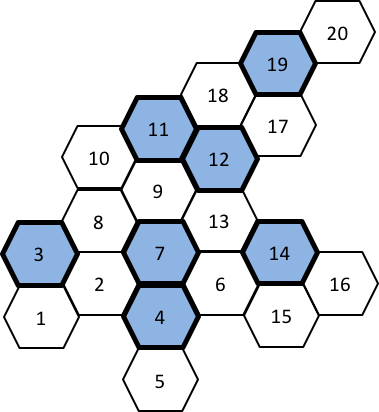
\includegraphics[scale=0.8]{chapters/chapter_8/figures/hive_setcover.png}
	\caption{The hive map illustrating the set covering problem. Our objective is to cover all of the regions while minimising the total cost incurred by opening the centres at the blue cells} \label{p1c8:fig:set_covering}
\end{figure}

To model the set covering problem, and pretty much any other problem involving indexed subsets such as $S_j$, $\forall j \in N$, we need an auxiliary parameter matrix $A$, often referred to as \emph{0-1 incidence matrix}. The matrix $A$ is such that
%
\begin{equation*}
	A = \begin{cases}
		A_{ij} = 1, \text{ if } i \in S_j, \\
		A_{ij} = 0, \text{ otherwise.}
	\end{cases}
\end{equation*}
%
For example, referring to Figure \ref{p1c8:fig:set_covering}, the first column of $A$ would refer to $j = 3$ and would have nonzero values at rows 1, 2, 3, and 8.

We are now ready to pose the set covering problem as an integer programming problem. For that, let $x_{j} = 1$ if a facility is opened (or a service centre is located) at location $j$ and $x_j = 0$, otherwise. In addition, let $M$ be the set of regions to be served and $N$ be the set of candidate places to have a facility opened. Then, the set covering problem can be formulated as follows.
%
\begin{align*}
  (SCP) : \mini_x \ & \sum_{j \in N} C_{j}x_{j} \\
  \st & \sum_{j \in N} A_{ij}x_{j} \geq 1, \ \forall i \in M\\
      & x_{j} \in \braces{0,1}, \ \forall j \in N. 
\end{align*}
%
As a final note, notice that this problem can also be posed as a combinatorial optimisation problem of the form
%
\begin{align*}
  \mini_{T \subseteq N} \braces{\sum_{j \in T} C_j : \bigcup_{j \in T}S_j = M},
\end{align*}
%
in which the locations $j \in T$ can be represented as an incidence vector, as before.


\subsection{Travelling salesperson problem}

The travelling salesperson problem (TSP) is one of the most famous combinatorial optimisation problems, perhaps due to its interesting mix of simplicity while being computationally challenging. Assume that we must visit a collection of $n$ cities at most once, and return to our initial point, forming a so-called \emph{tour}. When travelling from a city $i$ to a city $j$, we incur in the cost $C_{ij}$, representing, for example, distance or time. Our objective is to minimise the total cost of our tour. Notice that this is equivalent to finding the minimal cost permutation of $n-1$ cities, discarding the city which represents our starting and end point. Figure \ref{p1c8:fig:TSP} illustrates a collection of cities and one possible tour.

\begin{figure}[h]
	\centering
	\begin{tikzpicture}[node/.style={circle, fill=blue!60, draw, minimum size=1em, inner sep=2pt}, scale=1]
	    \node[node] (3) at (0, 0)  {3};
	    \node[node] (2) at (0, 1)  {2};
	    \node[node] (4) at (1, 0)  {4};
	    \node[node] (5) at (2, 0)  {5};
	    \node[node] (1) at (0, 2)  {1};
	    \node[node] (6) at (2, 2)  {6};     
	    \draw[->, thick] (1) -- (6);
	    \draw[->, thick] (6) -- (4);
	    \draw[->, thick] (4) -- (3);
	    \draw[->, thick] (3) -- (2);
	    \draw[->, thick] (2) -- (5);
	    \draw[->, thick] (5) -- (1);
	\end{tikzpicture}
	\caption{An example of a tour between the six cities} \label{p1c8:fig:TSP}
\end{figure}

To pose the problem as an integer programming model, let us define $x_{ij} =$ 1 if city $j$ is visited directly after city $i$, and $x_{ij} = 0$ otherwise. Let $N = \braces{1,\dots,n}$ be the set of cities. We assume that $x_{ii}$ is not defined for $i \in N$. A naive model for the travelling salesperson problem would be 
%
\begin{flalign*}
	(TSP) : \mini_x \ & \sum_{i \in N}\sum_{j \in N}C_{ij}x_{ij} \\
	\st & \sum_{j \in N \setminus \braces{i}} x_{ij} = 1, \ \forall i \in N\\
	& \sum_{i \in N \setminus \braces{j}} x_{ij} = 1, \ \forall j \in N\\
	& x_{ij} \in \braces{0,1}, \ \forall i,\forall j \in N : i \neq j
\end{flalign*}
%
First, notice that the proposed formulation of $TSP$ is exactly the same as that of the assignment problem. However, this formulation has an issue. Although it can guarantee that all cities are only visited once, it cannot enforce an important feature of the problem, which is that the tour cannot present disconnections, i.e., contain \emph{sub-tours}. In other words, the salesperson must physically visit from city to city when executing the tour and cannot ``teleport'' from one city to another. Figure \ref{p1c8:fig:TSP_subtours} illustrates the concept of sub-tours.

\begin{figure}[h]
	\centering	
	\begin{tikzpicture}[node/.style={circle, fill=blue!60, draw, minimum size=1em, inner sep=2pt}]
		\node[node] (1) at (0, 0) {1};
		\node[node] (2) at (0, 1) {2};
		\node[node] (3) at (1, 1) {3};
		\node[node] (4) at (1, 0) {4};
		\node[node] (5) at (2, 0) {5};
		\node[node] (6) at (2, 1) {6};			
		\draw[->] (1) -- (2);
		\draw[->] (2) -- (3);
		\draw[->] (3) -- (1);
		\draw[->] (4) -- (5);
		\draw[->] (5) -- (6);
		\draw[->] (6) -- (4);
	\end{tikzpicture}
	\caption{A feasible solution for the naive TSP model. Notice the two sub-tours formed} \label{p1c8:fig:TSP_subtours}
\end{figure}

In order to prevent sub-tours, we must include constraints that can enforce the full connectivity of the tour. There are mainly two types of such constraints. The first is called \emph{cut-set constraints} and is defined as
%
\begin{equation*} 
	\sum_{i \in S}\sum_{j \in N \setminus S}x_{ij} \geq 1, \ \forall S \subset N, 2 \leq |S| \leq n-1. 
\end{equation*}
%
The cut-set constraints act by guaranteeing that among any subset of nodes $S \subseteq N$ there is always at least one arc $(i,j)$ connecting one of the nodes in $S$ and a node not in $S$. 

An alternative type of constraint is called \emph{sub-tour elimination} constraint and is of the form
%
\begin{equation*}
	\sum_{i \in S}\sum_{j \in S}x_{ij} \leq |S|-1, \ \forall S \subset N, 2 \leq |S| \leq n-1. 
\end{equation*}
%
Differently from the cutset constraints, the sub-tour elimination constraints prevent the cardinality of the nodes in each subset from matching the cardinality of arcs within the same subset.

For example, consider the sub-tours illustrated in Figure \ref{p1c8:fig:TSP_subtours} and assume that we would like to prevent the sub-tour formed by $S = \braces{1,2,3}$. Then the cutset constraint would be of the form

\begin{equation*}
	x_{14} + x_{24} + x_{34} + x_{15} + x_{25} + x_{35} + x_{16} + x_{26} + x_{36}\geq 1	
\end{equation*}
%
while the sub-tour elimination would be of the form
\begin{equation*}
	x_{12} + x_{13} + x_{21} + x_{23} + x_{31} + x_{32} \leq 2
\end{equation*}
%
There are some differences between these two constraints. Typically, cutset constraints are preferred for being stronger (we will discuss the notion of stronger constraints in the next chapters). In any case, either of them suffers from the same problem: the number of such constraints quickly becomes computationally prohibitive as the number of nodes increases. This is because one would have to generate a constraint to each possible node subset combination from sizes 2 to $n-1$. 

A possible remedy to this consists of relying on \emph{delayed constraint generation}. In this case, one can start from the naive formulation $TSP$ and, from the obtained solution, check whether there are any sub-tours formed. That being the case, only the constraints eliminating the observed sub-tours need to be generated, and the problem can be warm-started. This procedure typically terminates far earlier than having all of the possible cutset or sub-tour elimination constraints generated. 


\subsection{Uncapacitated facility location}

This is the first mixed-integer programming model we consider. In this, we would like to design a network that can supply clients $i \in M$ by opening (or locating, as it is referred to in this context) facilities among candidate locations $j \in N$. Opening a facility incurs in the fixed cost $F_j$, and serving a client $i \in M$ from a facility that has been located at $j \in N$ costs $C_{ij}$. Our objective is to design the most cost-effective production and distribution network. That is, we must decide where to locate facilities and how to serve clients (from these facilities) with minimum total (locating plus service) cost. Figure \ref{p1c8:fig:facility_location_a} illustrates an example of the problem with $M = \braces{1,\dots,8}$ and $N = \braces{1,\dots,6}$ and Figure \ref{p1c8:fig:facility_location_b} presents one possible configuration with two facilities. The optimal number of facilities located and the client-facility association depends on the trade-offs between locating and service costs.	

\begin{figure}[h]
	\begin{subfigure}[b]{0.49\textwidth}
		\centering 
		\begin{tikzpicture}[scale = 0.5, 
	      	client/.style={circle, draw, fill=orange, minimum size=1em, inner sep=2pt},
	      	depot/.style={fill=blue!20, minimum size=1em, inner sep=2pt},
	      	located/.style={draw, fill=blue, minimum size=1em, inner sep=2pt}]
	          \node[client] (1) at (3,2) {$i_1$};
	          \node[client] (2) at (9,4) {$i_2$};
	          \node[client] (3) at (5,7) {$i_3$};
	          \node[client] (4) at (8,10) {$i_4$};
	          \node[client] (5) at (7,2) {$i_5$};
	          \node[client] (6) at (4,4) {$i_6$};
	          \node[client] (7) at (1,9) {$i_7$};
	          \node[client] (8) at (2,6) {$i_8$};
	          \node[depot]  (9) at (6,5) {$j_1$};
	          \node[depot] (10) at (6,9) {$j_2$};
	          \node[depot] (11) at (1,4) {$j_3$};
	          \node[depot] (12) at (5,1) {$j_4$};
	          \node[depot] (13) at (3,8) {$j_5$};
	          \node[depot] (14) at (9,6) {$j_6$};
	      \end{tikzpicture}
	      \caption{} \label{p1c8:fig:facility_location_a}	
	\end{subfigure}
	\hfill
	\begin{subfigure}[b]{0.49\textwidth}
		\centering
		\begin{tikzpicture}[scale = 0.5, 
	      	client/.style={circle, draw, fill=orange, minimum size=1em, inner sep=2pt},
	      	depot/.style={fill=blue!20, minimum size=1em, inner sep=2pt},
	      	located/.style={draw, fill=blue, minimum size=1em, inner sep=2pt}]
	          \node[client] (1) at (3,2) {$i_1$};
	          \node[client] (2) at (9,4) {$i_2$};
	          \node[client] (3) at (5,7) {$i_3$};
	          \node[client] (4) at (8,10) {$i_4$};
	          \node[client] (5) at (7,2) {$i_5$};
	          \node[client] (6) at (4,4) {$i_6$};
	          \node[client] (7) at (1,9) {$i_7$};
	          \node[client] (8) at (2,6) {$i_8$};
	          \node[depot]  (9) at (6,5) {$j_1$};
	          \node[depot] (10) at (6,9) {$j_2$};
	          \node[depot] (11) at (1,4) {$j_3$};
	          \node[depot] (12) at (5,1) {$j_4$};
	          \node[depot] (13) at (3,8) {$j_5$};
	          \node[depot] (14) at (9,6) {$j_6$};
	          \node[located] (11) at (1,4) {$j_3$};
	          \node[located] (9) at (6,5) {$j_1$};
	          \draw[-, thick] (4) -- (9);
	          \draw[-, thick] (3) -- (9);
	          \draw[-, thick] (2) -- (9);
	          \draw[-, thick] (5) -- (9);
	          \draw[-, thick] (6) -- (9);
	          \draw[-, thick] (8) -- (11);
	          \draw[-, thick] (6) -- (11);
	          \draw[-, thick] (1) -- (11);
	          \draw[-, thick] (7) -- (11);
	      \end{tikzpicture}
	      \caption{}\label{p1c8:fig:facility_location_b}
	\end{subfigure}
	\caption{An illustration of the facility location problem and one possible solution with two facilities located (right)}	
\end{figure}
 
To formulate the problem as a mixed-integer programming problem, let us define $x_{ij}$ as the fraction of the demand in $i \in M$ being served by a facility located at $j \in N$. In addition, we define the binary variable $y_j$ such that $y_j = 1$, if a facility is located at $j \in N$ and 0, otherwise. With those, the uncapacitated facility location (or UFL) problem can be formulated as 
%
\begin{flalign}
	(UFL) : \mini_{x,y} \ & \sum_{j \in N} F_jy_j +  \sum_{i \in M}\sum_{j \in N} C_{ij}x_{ij} \\
	\st & \sum_{j \in N} x_{ij} = 1, \ \forall i \in M\\
	& \sum_{i \in M} x_{ij} \leq m y_j, \ \forall j \in N \label{p1c8:eq:big-M_UFL}\\
	&x_{ij} \geq 0, \forall i \in M, \ \forall j \in N\\
	&y_j \in \braces{0,1}, \ \forall j \in N.
\end{flalign}

Some features of this model are worth highlighting. First, notice that the absolute values associated with the demand at nodes $i \in M$ are somewhat implicitly represented in the cost parameter $C_{ij}$. This is an important modelling feature that allows the formulation to be not only stronger but also more numerically favourable (avoiding large coefficients). Therefore, the demand is thought as being, at each node, 1 or 100\%, and $0 \le x_{ij} \le 1$ represents the fraction of the demand at $i \in M$ being served by a facility eventually located at $j \in N$. Second, notice how the variable $x_{ij}$ is only allowed to be greater than zero if the variable $y_j$ is set to 1, due to \eqref{p1c8:eq:big-M_UFL}. Notice that $m$, the number of clients, is acting as a maximum upper bound for the amount of demand being served from the facility $j$, which would be at most $m$ when only one facility is located. That constraint is precisely the reason why the problem is called uncapacitated, since, in principle, there are no capacity limitations on how much demand is served from a facility. 

Facility location problems are frequent in applications associated with supply chain planning problems and can be specialised to a multitude of settings, including capacitated versions (both nodes and arcs), versions where the arcs must also be located (or built), having multiple echelons, and so forth. 

 
\subsection{Uncapacitated lot-sizing}

Another example of an important mixed-integer programming formulation is the uncapacitated lot-sizing. In this, we would like to plan the production of a single product over a collection of time periods $T$. We have encountered this problem before in Chapter \ref{chapter_1}, but now we consider the variation in which the production activity implies in a fixed cost $F_t$, representing, for example, a setup cost or the need for renting equipment. Once again, for each period $t \in T$, we incur a cost $C_t$ to produce one unit in period $t$ and $H_t$ is paid to store one unit of product from period $t$ to period $t+1$.

Let us define $p_t \geq 0$ be the amount produced in period $t \in T$, and $s_t \geq 0$ as the amount stored at the end of period $t \in T$. In addition, let $y_t \in \braces{0,1}$ indicate whether production occurs in period $t \in T$. Also, assume that $M$ is a sufficiently large constraint. Then, the uncapacitated lot-sizing (ULS) can be formulated as
%
\begin{align}
	(ULS) : \mini_{x,s,y} \ & \sum_{t \in N} (F_ty_t + P_tp_t + H_ts_t) \nonumber \\
	\st & s_{t-1} + p_t = d_t + s_t, \ \forall t \in N \nonumber \\
	& p_t \leq My_t, \ \forall t \in N  \label{p1c8:eq:big_M_ULS}\\
	&s_t, p_t \geq 0, \ \forall t \in N \nonumber \\
	&y_t \in \braces{0,1}, \ \forall t \in N. \nonumber
\end{align} 

Notice that the formulation of $ULS$ is very similar to that seen in Chapter \ref{chapter_1}, with exception of the variable $y_t$, its associated fixed cost term $\sum_{t \in T} F_jy_j$ and the constraint \eqref{p1c8:eq:big_M_ULS}. This constraint is precisely what renders the ``uncapacitated'' nomenclature, and is commonly known in the context of mixed-integer programming as \emph{big-M constraints}. Notice that the constant $M$ is playing the role of $+\infty$: it only really makes the constraint relevant when $y_t = 0$, so that $p_t \le 0$ is enforced, making thus $p_t = 0$. However, this interpretation has to be taken carefully. Big-M constraints are known for being the cause of numerical issues and worsening the performance of mixed-integer programming solver methods. Thus, the value of $M$ must be set such that it is the smallest value possible such that it does not artificially create a constraint. Finding these values are often challenging and instance dependent. In the capacitated case, $M$ can trivially take the value of the production capacity. 
 
  
\section{Good formulations}

In this section, we discuss what makes a formulation a better formulation for a (mixed-)integer programming (MIP) problem. Just like it is the case with any mathematical programming application, there are potentially infinite possible ways to formulate the same problem. While in the case of linear programming (i.e., only continuous variables), alternative formulations typically do not lead to significant differences in terms of computational performance, the same is definitely not true in the context of MIP. In fact, whether a MIP problem can be solved in a reasonable computational time often depend on having a good, or \emph{strong}, formulation.

Therefore, we must be able to recognise, from a set of equivalent formulations for the same problem, that which yields better computational performance. But first, we must be able to understand the source of these differences in computational performance. For that, the first thing to realise is that solution methods for MIP models rely on \emph{successively solving linear programming models} called \emph{linear programming (LP) relaxations}. How exactly this happens will be the subject of our next chapters. But for now, one can infer that the best formulation will be the one that requires the solution of the least of such LP relaxations. And precisely, it so turns out that the number of LP relaxations that need to be solved (and, hence, performance) is strongly dependent on how closely the formulation resembles the \emph{convex hull} of the feasible solutions.

An LP relaxation simply consists of a version of the original MIP problem in which the integrality requirements are dropped. Most of the methods used to solve MIP models are based on LP relaxation. There are several reasons why the employment of LP relaxations is a good strategy. First, we can solve (and resolve) LP problems efficiently. Secondly, the solution of the LP relaxation can be used to \emph{reduce} the search space of the original MIP. However, simply rounding the solution of the LP relaxation will typically not lead to relevant solutions.

Let us illustrate the geometry of an integer programming model, such that the points we were discussing become more evident. Consider the problem
%
\begin{align*}
	(P): \maxi_x &x_1 + \frac{16}{25}x_2 \\
	\st &50x_1 + 31x_2 \leq 250\\
	&3x_1 + 31x_2 \geq -4\\
	&x_1, x_2 \in \integers_+.
\end{align*}
 
The feasible region of problem $P$ is represented in Figure \ref{p1c8:fig:IP_feasible_region}. First, notice how in this case the feasible region is not a polyhedral set anymore, but yet a collection of discrete points (represented in blue) that happen to be within the polyhedral set formed the linear constraints. This is one of the main complicating features of MIPs because the premise of convexity does not hold anymore. 

Figure \ref{p1c8:fig:IP_feasible_region} also illustrates how rounding the solution obtained from the LP relaxation would, as it is often the case with MIPs, lead to infeasible solutions, except when $x_1$ is rounded up and $x_2$ rounded down, which leads to the suboptimal solution $(2,5)$. However, one can still graphically find the optimal solution using the same procedure as that employed for linear programming problems, which would lead to the optimal integer solution $(5,0)$.

\begin{figure}[h]
	\begin{tikzpicture}[scale = 0.65,
		  point/.style={circle, fill=gray!40, inner sep=1pt},
		  feas point/.style={circle, fill=blue, inner sep=1pt}]
		  \foreach \x in {0,...,6}{
		      \foreach \y in {0,...,6} {
		          \node[point] (\x,\y) at (\x, \y) {};
		      }}
		  \foreach \x in {0,...,6}{
		      \node[font=\scriptsize] at (\x,-0.5) {$\x$};
		  }
		  \foreach \y in {0,...,6}{
		      \node[font=\scriptsize] at (-0.5,\y) {$\y$};
		  }                      
		  \draw[thick, <->] (7,0) node[below]{$x_1$} -- (0,0) -- (0,7) node[left]{$x_2$};  
		  \draw[domain=1:5, thick,variable=\x,blue] plot ({\x},{250/31 - 50/31*\x});  
		  \draw[domain=0:3, thick,variable=\x,blue] plot ({\x},{2 + 3/2*\x});
		  \node[circle, fill=orange, inner sep=2pt] at (5,0) {};   
		  \node[font=\scriptsize, inner sep=2pt, above right] at (5,0) {opt. IP sol};   
		  \node[fill=orange, inner sep=2pt] at (376/193, 950/193){};
		  \node[font=\scriptsize, above right, inner sep=2pt] at (376/193, 950/193){LP sol. (376/193, 950/193)};
		\node[feas point] at (0,0){};
		\node[feas point] at (0,1){};
		\node[feas point] at (0,2){};
		\node[feas point] at (1,0){};
		\node[feas point] at (1,1){};
		\node[feas point] at (1,2){};
		\node[feas point] at (1,3){};    
		\node[feas point] at (2,0){};
		\node[feas point] at (2,1){};
		\node[feas point] at (2,2){};
		\node[feas point] at (2,3){};
		\node[feas point] at (2,4){};
		\node[feas point] at (3,0){};
		\node[feas point] at (3,1){};
		\node[feas point] at (3,2){};
		\node[feas point] at (3,3){};
		\node[feas point] at (4,0){};
		\node[feas point] at (4,1){};                            
	\end{tikzpicture}
	\caption{Graphical representation of the feasible region of the example}	 \label{p1c8:fig:IP_feasible_region}
\end{figure}


\subsection{Comparing formulations}

In order to be able to compare formulations, we require some specific definitions, including a precise definition of what is a \emph{formulation}.

\begin{definition} \label{p1c8:def:formulation}
	A polyhedral set $P = \braces{x \in \reals^{n+p} : Ax \leq b}$ is a formulation for a set $X \subseteq \integers^n \times \reals^p $ if and only if $X = P \cap (\integers^n \times \reals^p)$.
\end{definition}

From Definition \ref{p1c8:def:formulation}, we can conclude that two formulations $P_1$ and $P_2$ are \emph{equivalent} if $P_1 \cap (\integers^n \times \reals^p) = P_2 \cap (\integers^n \times \reals^p)$. Moreover, from Definition \ref{p1c8:def:formulation}, it becomes clear that the feasible region of an integer programming problem is a collection of points represented by $X$. This is illustrated in Figure \ref{p1c8:fig:alternative_formulations}, where one can see three alternative equivalent formulations, $P_1$, $P_2$, and $P_3$ for the same set $X$.

\begin{figure}[h]
	\begin{tikzpicture}[scale = 0.8,
	point/.style={circle, fill=gray!40, inner sep=1pt},
	feas point/.style={circle, fill=blue, inner sep=1pt}]
		\draw[blue] (3.2, 4.5) -- (1.5, 3.5) -- (1.5,1.5) -- (3.5, 1.5) -- (4.5, 2.5)     -- cycle;
		\draw[orange] (2.5, 1.5) -- (1, 2.5) -- (2.5,4.5) -- (4, 3.5) -- (4.75, 2) -- cycle;
		\draw[teal] (2, 2) -- (2, 3) -- (3, 4) -- (4, 3) -- (4, 2) -- cycle;  
		\foreach \x in {0,...,5}{
		  \foreach \y in {0,...,5} {
		      \node[point] (\x,\y) at (\x, \y) {};
		  }}
		\foreach \x in {0,...,5}{
		  \node[font=\scriptsize] at (\x,-0.4) {$\x$};
		}
		\foreach \y in {0,...,5}{
		  \node[font=\scriptsize] at (-0.4,\y) {$\y$};
		}                      
		\draw[thick, <->] (5.5,0) node[below]{$x_1$} -- (0,0) -- (0,5.5) node[left]{$x_2$};             
		\node[feas point] at (2,2){};
		\node[feas point] at (3,2){};
		\node[feas point] at (2,3){};
		\node[feas point] at (3,3){};
		\node[left] at (3,3){\color{teal}{$P_3$}};
		\node[above] at (2.5,4.5){\color{orange}{$P_2$}};
		\node[above] at (3.5,4.5){\color{blue}{$P_1$}};
		\node[feas point] at (3,4){};
		\node[feas point] at (4,3){};
		\node[feas point] at (4,2){};
	\end{tikzpicture}
	\caption{An illustration of three alternative formulations for $X$. Notice that $P_3$ is an ideal formulation, representing the convex hull of $X$.} \label{p1c8:fig:alternative_formulations}
\end{figure}

Formulation $P_3$ has a special feature associated with it. Notice how all extreme points of $P_3$ belong to $X$. This has an important consequence. That implies that the solution of the original integer programming problem can be obtained by solving a single LP relaxation since the solution of both problems is the same. This is precisely what characterises an \emph{ideal} formulation, which is that leading to a minimal (i.e., only one) number of required LP relaxation solutions as solving an LP relaxation over an ideal $P$ yields a solution $x \in X$ for any cost vector $c$. This will only be the case if the formulation $P$ is the \emph{convex hull} of $X$.

This is the case because of two important properties relating to the set $X$ and its convex hull $\conv(X)$. The first is that $\conv(X)$ is a polyhedral set, and the second is that the extreme points of $\conv(X)$ belong to $X$. We summarise those two facts in Proposition \ref{p1c8:prop:polyhedra_convex_hull}, to which we will refer shortly. Notice that the proof for the proposition can be derived from Definition \ref{p1c2:def:convex_combination_hull} and Theorem \ref{p1c2:thm:convexity}, and is left as an exercise.
  
\begin{proposition}\label{p1c8:prop:polyhedra_convex_hull}
	$\conv(X)$ is a polyhedral set and all its extreme points belong to $X$. 
\end{proposition}

%TODO: Chp8: add a proof.
 
If $P$ is such that $P = \conv (X)$, the original problem 
%
\begin{equation*}
	\mini\braces{c^\top x : x \in X},
\end{equation*}
%
can, in principle, be replaced with 
%
\begin{equation*}
	\mini\braces{ c^\top x : x \in \conv(X)},	
\end{equation*}
%
where we have that 
%
\begin{equation*}
	X = \braces{Ax \leq b, x \in \integers^n \times \reals^p} \text{ and } \conv(X) = \braces{Ax \leq b, x \in \reals_+^{n+p}}.	
\end{equation*}

Unfortunately, this is often not the case. Typically, except for some specific cases, a description of $\conv(X)$ is not known and deriving it algorithmically is an impractical computational task. However, Proposition \ref{p1c8:prop:polyhedra_convex_hull} allows us to define a structured way to compare formulations. This is summarised in Definition \ref{p1c8:def:better_formulations}.

\begin{definition} \label{p1c8:def:better_formulations}
  Given a set $X\subseteq \integers^n\times\reals^n$ and two formulations $P_1$ and $P_2$ for $X$, $P_1$ is a \emph{better formulation} than $P_2$ if $P_1 \subset P_2$. 
\end{definition}

Definition \ref{p1c8:def:better_formulations} gives us a framework to try to demonstrate that a given formulation is better than another. If we can show that $P_1 \subset P_2$, then, by definition (literally), $P_1$ is a better formulation than $P_2$. Clearly, this is not a perfect framework, since, for example, it would not be useful for comparing $P_1$ and $P_2$ in Figure \ref{p1c8:fig:alternative_formulations}, and, in fact, there is nothing that can be said a priori about the two in terms of which will render the better performance. Often, in the context of MIP, this sort of analysis can only rely on careful computational experimentation. 

A final point to make is that sometimes one must compare formulations of distinct dimensions, that is, with a different number of variables. When that is the case, one can resort to projection, as a means to compare both formulations onto the same space of variables. 

\newpage
\section{Exercises}

\subsection*{Exercise 8.1: Uncapacitated lot sizing (ULS) formulations}
Consider the following formulations $P_{\text{ULS-1}}^{(x,s,y)}$ and $P_{\text{ULS-2}}^{(w,y)}$ as linear (i.e., continuous) relaxations for the ULS problem defined over $N = \{1,\dots,n\}$ periods:
\renewcommand*{\arraystretch}{1.1}
\[P_{\text{ULS-1}}^{(x,s,y)} = \left\{
  \begin{array}{llr}
  	(x,s,y): & s_{t-1} + x_t = d_t + s_t, & \forall t\in N\\
    	     & x_t  \leq M y_t, 		  & \forall t\in N\\
    	     & s_0 = 0, 			      & 			  \\
    	     & s_t \geq 0, 				  & \forall t\in N\\
    	     & x_t \geq 0, 			      & \forall t\in N\\
    	     & 0 \leq y_{t} \leq 1, 	  & \forall t\in N
  \end{array}\right\}
  \quad~\left|
  \begin{array}{rr}
  	x_t  & \text{production in period } t\\
    s_t  & \text{stock in period }      t\\
    y_t  & \text{setup in period }      t\\[5pt]
    d_t  & \text{demand in period }     t\\
    M    & \text{maximum production}\\
%         & \text{capacity}\\
         & M = \sum_{t\in N}d_t
  \end{array}\right.
\]\\[-30pt]


\[~~~P_{\text{ULS-2}}^{(w,y)} = \left\{
  \begin{array}{llr}
    (w,y): & \sum \limits_{i=1}^t w_{it} = d_t, &\forall t\in N\\
    	   & w_{it} \leq d_t y_i,  				&\forall i,t\in N : i\leq t\\
    	   & w_{it} \geq 0,        				&\forall i,t\in N : i\leq t\\
    	   & 0 \leq y_{t} \leq 1,  				&\forall t\in N 
  \end{array}\right\}
  \quad~~\left|
  \begin{array}{rr}
  	w_{it} & \text{production in period } i\\
      	   & \text{to be used in period } t\\[3pt]
       y_t & \text{setup in period } t\\
       	   & \\[7pt] 
  \end{array}\right.
\]

\vspace{5pt}

(a) Use projection to show that $P_{\text{ULS-2}}^{(w,y)}$ is stronger than $P_{\text{ULS-1}}^{(x,s,y)}$, i.e, $P_{\text{ULS-2}}^{(w,y)} \subset P_{\text{ULS-1}}^{(x,s,y)}$.

\emph{Hint:} 
First, construct an extended formulation $P_{\text{ULS-2}}^{(x,s,y,w)}$ by writing the variables $x_t$ and $s_t$ in terms of variables $w_{it}$ and add them to $P_{\text{ULS-2}}^{(w,y)}$. Then, use a projection to show that 
\begin{equation*}
\proj_{x,s,y}\,(P_{\text{ULS-2}}^{(x,s,y,w)}) \subseteq P_{\text{ULS-1}}^{(x,s,y)},
\end{equation*} 
which is equivalent to $P_{\text{ULS-2}}^{(w,y)} \subseteq P_{\text{ULS-1}}^{(x,s,y)}$. Do this by verifying that each constraint of $P_{\text{ULS-1}}^{(x,s,y)}$ is satisfied by all $(x,s,y)\in P_{\text{ULS-2}}^{(x,s,y,w)}$. Finally, show that a solution $(\bar{x},\bar{s},\bar{y})$ with $\bar{x}_t = d_t$ and \lb $\bar{y}_t = d_t/M$, for all $t \in N$, satisfies $(\bar{x},\bar{s},\bar{y}) \in P_{\text{ULS-1}}^{(x,s,y)} \setminus P_{\text{ULS-2}}^{(x,s,y,w)}$.

\vspace{5pt}

(b) The optimisation problems associated with the two ULS formulations are
\begin{align*}
	\begin{array}{lrlr}
		\text{(ULS-1)} & \mini\limits_{x,s,y} & \sum\limits_{t\in N} (f_ty_t + p_tx_t + q_ts_t)\\
		         & \st  & s_{t-1} + x_t = d_t + s_t, & \forall t\in N\\
		    	 &      & x_t  \leq M y_t, 		  & \forall t\in N\\
		    	 &      & s_0 = 0, 			      & 			  \\
		    	 &      & s_t \geq 0, 			  & \forall t\in N\\
		    	 &      & x_t \geq 0, 			  & \forall t\in N\\
		    	 &      & 0 \leq y_{t} \leq 1, 	  & \forall t\in N
	 \end{array}
	 \quad~\left|
	 \begin{array}{rr}
	  	x_t  & \text{production in period } t\\
	    s_t  & \text{stock in period }      t\\
	    y_t  & \text{setup in period }      t\\[5pt]
	    d_t  & \text{demand in period }     t\\
	    M    & \text{maximum production}\\
	 %         & \text{capacity}\\
	         & M = \sum_{t\in N}d_t
	 \end{array}\right.
\end{align*}\\[-30pt]

\begin{align*}
	\begin{array}{lrlr}
		\text{(ULS-2)} & \mini\limits_{w,y} & \multicolumn{2}{c}{\sum \limits_{t \in N} \brackets{f_ty_t + p_t\sum \limits_{i=t}^{n}w_{ti} + q_t\sum\limits_{i=1}^{t}\left(\sum \limits_{j=i}^{n}w_{ij} - d_i\right)}}\\
		               & \st                & \sum \limits_{i=1}^t w_{it} = d_t, &\forall t\in N\\              
		    	       &                    & w_{it} \leq d_t y_i,  			 &\forall i,t\in N : i\leq t\\  
		    	       &                    & w_{it} \geq 0,        			 &\forall i,t\in N : i\leq t\\  
		    	       &                    & 0 \leq y_{t} \leq 1,  			 &\forall t\in N                   
    \end{array}
    \quad~\left|
    \begin{array}{rr}
 	  	w_{it} & \text{production in period } i\\
 	      	   & \text{to be used in period } t\\%[3pt]
 	       y_t & \text{setup in period } t\\
 	       	   & %[20pt] 
    \end{array}\right.
\end{align*}\\[-20pt]

Consider a ULS problem instance over $N = \{1,\dots,6\}$ periods with demands $d = (6,7,4,6,3,8)$, set-up costs $f = (12,15,30,23,19,45)$, unit production costs $p = (3,4,3,4,4,5)$, unit storage costs \lb $q = (1,1,1,1,1,1)$, and maximum production capacity $M = \sum_{i=1}^6d_j = 34$. Solve the problems ULS-1 and ULS-2 with Julia using JuMP to verify the result of part (a) computationally.

\subsection*{Exercise 8.2: TSP formulation - MTZ}
Show that the following formulation $P_{MTZ}$ is valid for the TSP defined on a directed graph \lb $G = (N,A)$ with $N = \{1,\dots,n\}$ cities and arcs $A = \{(i,j) : i,j\in N, i\neq j\}$ between cities.
\renewcommand*{\arraystretch}{1.3}
\[P_{MTZ} = \left\{
   \begin{array}{ll}
   \displaystyle \sum_{j \in N \setminus \{i\}} x_{ij} = 1, & \forall i \in N \\
   \displaystyle \sum_{j \in N \setminus \{i\}} x_{ji} = 1, & \forall i \in N \\   
   \displaystyle u_{i} - u_{j} + (n-1) x_{ij} \leq n - 2, & \forall i,j \in N \setminus \{ 1 \} : i \neq j ~~(*)\\
    x_{ij} \in \{0,1\}, & \forall i,j \in N : i\neq j\\
  \end{array}
\right.
\]
where $x_{ij} = 1$ if city $j\in N$ is visited immediately after city $i \in N$, and $x_{ij} = 0$ otherwise. Constraints $(*)$ with the variables $u_i \in \reals$ for all $i\in N$ are called \emph{Miller-Tucker-Zemlin} (MTZ) subtour elimination constraints. 

\emph{Hint:} Formulation $P_{MTZ}$ is otherwise similar to the formulation presented, except for the constraints $(*)$ which replace either the cutset constraints
$$\sum_{i \in S}\sum_{j \in N \setminus S}x_{ij} \geq 1, \ \forall S \subset N, S \neq \emptyset,$$
or the subtour elimination constraints        
$$\sum_{i \in S}\sum_{j \in S}x_{ij} \leq |S|-1, \ \forall S \subset N, 2 \leq |S| \leq n-1,$$
which are used to prevent subtours in TSP solutions. Thus, you have to show that: 
\begin{enumerate}
	\item[(1)] Constraints $(*)$ prevent subtours in any solution $x\in P_{MTZ}$.
	\item[(2)]Every TSP solution $x$ (on the same graph $G$) satisfies the constraints $(*)$.
\end{enumerate}
You can prove (1) by contradiction. First, assume that a solution $x\in P_{MTZ}$ has a subtour with $k$ arcs $(i_1,i_2),\dots,(i_{k-1},i_k),(i_k,i_1)$ and $k$ nodes $\{i_1,\dots,i_k\} \in N\setminus\{1\}$. Then, write the constraints $(*)$ for all arcs in this subtour and try to come up with a contradiction.

You can prove (2) by finding suitable values for each $u_2,\dots,u_n$ that will satisfy the constraints $(*)$ for any TSP solution $x$. Recall that a TSP solution represents a \emph{tour} that visits each of the $N = \{1,\dots,n\}$ cities exactly once and returns to the starting city.


\subsection*{Exercise 8.3: TSP implementation}
Solve a 15 node TSP instance using the formulation $P_{MTZ}$ presented in Exercise 8.1. You can randomly generate city coordinates in xy-plane for all $N = \{1,\dots,n\}$ cities. Letting $c_{ij}$ denote the distance between cities $i$ and $j$, the problem $MTZ$ can be formulated as
%
\begin{align*}
	(MTZ) : \mini_{x,u} & ~~\,\sum_{i\in N}\sum_{j\in N} c_{ij}x_{ij}\\
		    \st & \sum_{j \in N \setminus \{i\}} x_{ij} = 1, & \forall i \in N, \\
		        & \sum_{j \in N \setminus \{i\}} x_{ji} = 1, & \forall i \in N, \\   
		        & ~~\,u_{i} - u_{j} + (n-1) x_{ij} \leq n - 2, & \forall i,j \in N \setminus \{ 1 \} : i \neq j,\\
		        & ~~\,x_{ij} \in \{0,1\}, & \forall i,j \in N : i\neq j.
\end{align*}
%
Implement the model and solve the problem instance with Julia using JuMP.

\subsection*{Exercise 8.4: TSP formulation - tightening the MTZ formulation}
Recall the MTZ formulation for the Travelling Salesperson Problem (TSP) presented in Exercise 8.2. 

(a) Show that the inequalities \eqref{eq:31} - \eqref{eq:34} are valid for the TSP problem (i.e., they hold for any feasible solution of the TSP problem), assuming that $n > 2$:

\begin{align}
&x_{ij} + x_{ji} \leq 1, &\forall i,j \in N : i\neq j\qquad\label{eq:31}\\[5pt]
&u_i - u_j + (n-1)x_{ij} + (n-3)x_{ji} \leq n-2,   &\forall i,j \in N\setminus\{1\} : i \neq j\qquad\label{eq:32}\\[5pt]
&u_j - 1 + (n-2)x_{1j} \leq n - 1 &\forall j \in N\setminus\{1\}\qquad\\[5pt]
&1 - u_i + (n-1)x_{i1} \leq 0 &\forall i \in N\setminus\{1\}\qquad\label{eq:34}
\end{align}

\emph{Hint:} You can assume that the variables $u_2,\dots,u_n$ take unique integer values from the set $\{2,\dots,n\}$. That is, we have $u_i\in \{2,\dots,n\}$ for all $i = 2,\dots,n$ with $u_i \neq u_j$ for all $i,j\in 2,\dots,n$. This holds for any TSP solution of problem MTZ as we showed in Exercise 8.2. If we fix city 1 as the starting city, then the value of each $u_i$ represents the position of city $i$ in the TSP tour, i.e., $u_i = t$ for $t = 2,\dots,n$ if city $i\neq1$ is the $t$:th city in the tour. You have to check that each of the inequalities \eqref{eq:31} - \eqref{eq:34} hold (individually) for any arc $(i,j)\in A$ and city $i\in N$ that are part of the inequality, by checking that the following two cases are satisfied: either $x_{ij} = 0$ or $x_{ij} = 1$.


(b) Add all four sets of inequalities \eqref{eq:31} - \eqref{eq:34} to the MTZ formulation and compare the computational performance against the model with no extra inequalities.
%\emph{Hint:} The inequalities \eqref{eq:32} \emph{dominate} the original subtour elimination constraints \eqref{eq:MTZ}, so you can also try to solve the problem by commenting over the original constraints \eqref{eq:MTZ} after adding the valid inequalities \eqref{eq:32}. 


\subsection*{Exercise 8.5: Scheduling problem}
A set of $N = \{1,\dots,n\}$ jobs must be carried out on a single machine that can do only one job at a time. Each job $j\in N$ takes $p_j$ hours to complete. Given job weights $w_j$ for all $j\in N$, in what order should the jobs be carried out so as to minimise the weighted sum of their start times? Formulate this scheduling problem as a mixed integer-programming problem. 

%\emph{Hint:} Use variables $t_j \geq 0$ to represent start times of each job $j$, and variables $x_{ij} \in \{0,1\}$ with $x_{ij} = 1$ if job $i$ precedes job $j$ and $x_{ij} = 0$ otherwise.  

\subsection*{Exercise 8.6: Piecewise linear objective functions and logical constraints}
Recall the paint factory problem 
%
\begin{flalign}
	\maxi z = \ & 5x_1 + 4x_2 \label{p1c1:eq:constM1}\\
	\st & 6x_1 + 4x_2 \leq 24 \label{p1c1:eq:constM2}\\
	& x_1 + 2x_2 \leq 6 \\
	& x_2 - x_1 \leq  1 \\
	& x_2 \leq 2 \\
	& x_1, x_2 \geq 0,
\end{flalign}
%
where $x_1$ representes the amount (in tons) of exterior paint produced, and $x_2$ the amount of interior paint produced. This is a simple linear problem that has been used as an illustrative example throughout the lecture notes. 

To demonstrate some typical structures in integer programming models, we now add two modifications to the problem, namely
%
\begin{itemize}
    \item Piecewise linear functions: the profit for exterior paint depends on the amount produced. The profit for the first ton produced is 7 (\$1000/ton), while the next ton can only be sold at a profit of 5, the third for a profit of 3 and the fourth ton only makes a profit of 1. 
    \item Logical constraints: the factory has to produce at least 1.5 tons of at least one of the two paint types, that is, either $x_1 \ge 1.5$ or $x_2 \ge 1.5$ must hold.
\end{itemize}

As seen in Fig. \ref{p1c8:fig:E86-plot}, these modifications result in a nonlinear objective function and a nonconvex feasible region. Using additional integer/binary variables, formulate and solve the problem as a mixed-integer linear problem.

\begin{figure}[h]
	\centering
	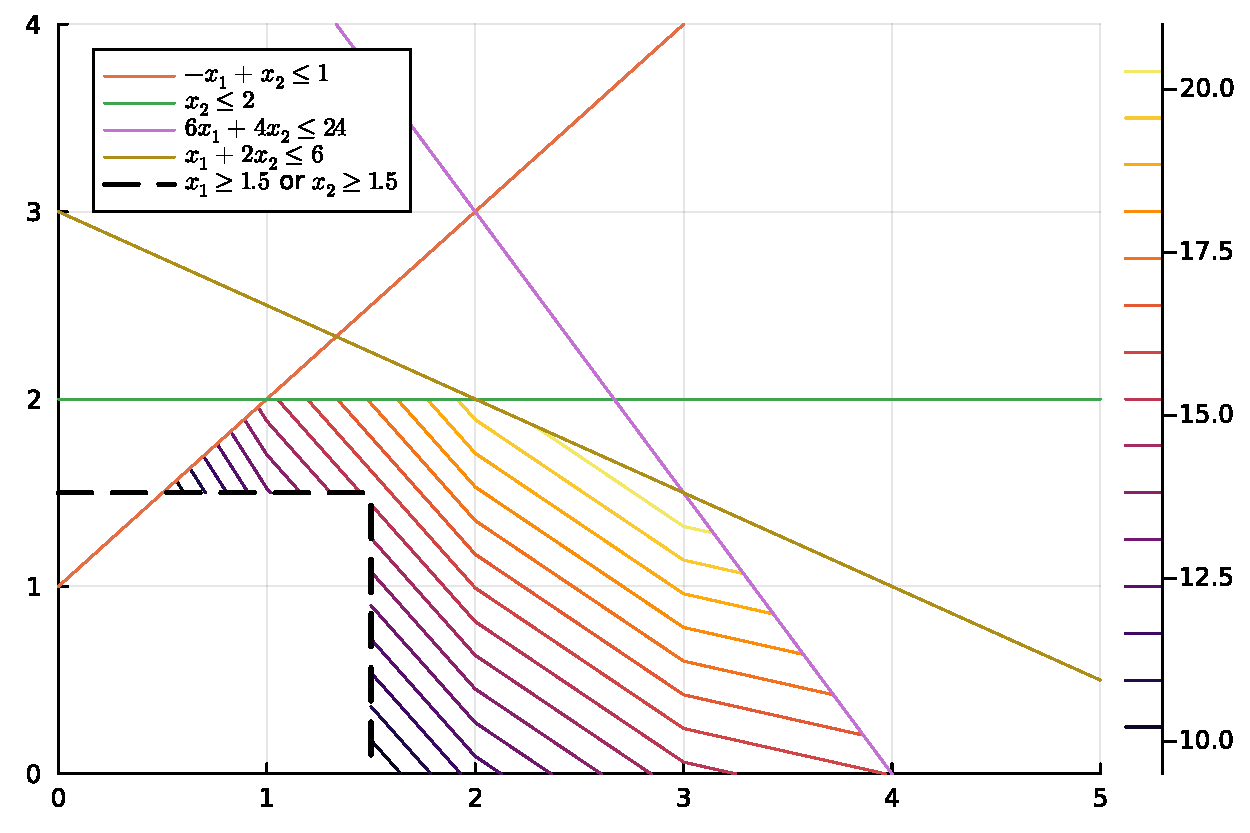
\includegraphics[width=0.5\textwidth]{chapters/chapter_8/figures/E86-plot.pdf}
	\caption{The feasible region of the problem, and the contours of the objective function} 
    \label{p1c8:fig:E86-plot}
\end{figure}


	
	\chapter{Branch-and-bound Method} \label{chapter_9}
	% TODO: Chp9: make it uniform the notation for sets (polyhedral set P clashes with problem P)

\section{Optimality for integer programming problems}

We will now discuss a method to solve mixed-integer programming problems that rely on the successive solution of linear programming relaxations. Although there are several methods that can be employed to solve combinatorial optimisation problems, often they are not capable of providing optimality guarantees for the solution obtained (e.g., are heuristics or metaheuristics) or do not exploit the availability of a (linear) mathematical programming formulation. To date, the most widespread method capable of both is generally known as a \emph{branch-and-cut} method.

Branch-and-cut methods are composed of a combination of multiple parts, including, among other techniques, a branch-and-bound coordination scheme, cutting planes, and heuristics as well. In the next chapters, we will focus on each of these parts individually, starting with the \emph{branch-and-bound} method.


\section{Relaxations}

Before we present the method itself, let us discuss the more general concept of \emph{relaxation}. We have visited the concept somewhat informally before, but now we will concentrate on a more concrete definition.

Consider an integer programming problem of the form
%
\begin{equation*}
	z = \mini_x \braces{c^\top x : x \in X \subseteq \integers^n}.
\end{equation*}
%
To prove that a given solution $x^*$ is optimal, we must rely on the notion of \emph{bounding}. That is, we must provide a pair of upper and lower bounds that are as close (or tight) as possible. If it happens that these bounds have the same value, and thus match the value of $z = c^\top x^*$, we have available a \emph{certificate} of optimality for $x^*$. This concept must sound familiar to you. We already used similar arguments in Chapter \ref{chapter_5}, when we introduced the notion of dual bounds.

Most methods that can prove optimality work by bounding the optimal solution. In this context, bounding means to construct an increasing sequence of lower bounds
%
\begin{equation*}
	\underline{z}_1 < \underline{z}_2 < \dots < \underline{z}_s \leq z	
\end{equation*}
%
and a decreasing sequence of upper bounds
%
\begin{equation*}
	\overline{z}_1 > \overline{z}_2 > \dots > \overline{z}_t \geq z
\end{equation*}
%
to obtain as tight as possible lower ($\underline{z} \leq z$) and upper ($\overline{z} \geq z$) bounds. Notice that the process can be arbitrarily stopped when $\overline{z}_t - \underline{z}_s \leq \epsilon$, where $s$ and $t$ are some positive integers and $\epsilon > 0$ is a predefined (suitably small) tolerance. The term $\epsilon$ represents an \emph{absolute optimality gap}, meaning that one can guarantee that the optimal value is at most greater than $\underline{z}$ by $\epsilon$ units and at most smaller than $\overline{z}$ by $\epsilon$ units. In other words, the optimal value must be either $\underline{z}$, $\overline{z}$, or a value in between.

This framework immediately poses the challenge of deriving such bounds efficiently. It turns out that this is a challenge that goes beyond the context of mixed-integer programming problems. In fact, we will see this idea of bounding in Chapter \ref{chapter_12} when we discuss decomposition methods, which also generate lower and upper bounds during their execution.

Regardless of the context, bounds are typically of two types: \emph{primal} bounds, which are bounds obtained by evaluating a \emph{feasible} solution (i.e., that satisfy primal feasibility conditions); and \emph{dual} bounds, which are typically attained when primal feasibility is allowed to be violated so that a dual feasible solution is obtained. In the context of minimisation, primal bounds are upper bounds (to be minimised), while dual bounds are lower bounds (to be maximised). Clearly, in the case of maximisation, the reverse holds. 

Primal bounds can be obtained by means of a feasible solution. For example, one can heuristically assemble a solution that is feasible by construction. On the other hand, dual bounds are typically obtained by means of solving a \emph{relaxation} of the original problem. We are ready now to provide Definition \ref{p1c9:def:relaxation}, which formally states the notion of relaxation.

\begin{definition}[Relaxation] \label{p1c9:def:relaxation}
	Problem 
	%
	\begin{equation*}
	  (RP): z_{RP} = \mini \braces{\overline{c}^\top x : x \in \overline{X} \subseteq \reals^n} 
	\end{equation*}
%
	is a relaxation of problem
	%
	\begin{equation*}
	  (P): z = \mini \braces{c^\top x : x \in X \subseteq \reals^n} 
	\end{equation*}
	%
	if $X \subseteq \overline{X}$, and $\overline{c}^\top x \leq c^\top x$, $\forall x \in X$.
\end{definition}

Definition \ref{p1c9:def:relaxation} provides an interesting insight related to relaxations: they typically comprise an expansion of the feasible region, possibly combined with an objective function bounding. Thus, two main strategies to obtain relaxations are to enlarge the feasible set by dropping constraints and replacing the objective function with another of the same or smaller value. One might notice at this point that we have used a very similar argumentation to define linear programming duals in Chapter \ref{chapter_5}. %We will return to the relationship between relaxations and Lagrangian duality in a more general setting in Part \ref{part_2}, when we discuss the notion of Lagrangian relaxation.

Clearly, for relaxations to be useful in the context of solving mixed-integer programming problems, they have to be easier to solve than the original problem. That being the case, we can then rely on two important properties that relaxations have, which are crucial for using them as a means to generate dual bounds. These are summarised in Proposition \ref{p1c9:prop:relaxation_bounding} and \ref{p1c9:prop:relaxation_optimality}.

\begin{proposition} \label{p1c9:prop:relaxation_bounding}
	If RP is a relaxation of P, then $z_{RP}$ is a dual bound for $z$. 
\end{proposition}
    
\begin{proof} Let $x^*_{RP}$ be the optimal solution for $RP$. For any optimal solution $x^*$ of $P$, we have that $x^* \in X \subseteq \overline{X}$, which implies that $x^* \in \overline{X}$. Thus, we have that
  \begin{equation*}
  	 z = c^\top x^* \geq \overline{c}^\top x^* \geq \overline{c}^\top x^*_{RP} = z_{RP}.	\qedhere
  \end{equation*}
\end{proof}

The first inequality is due to Definition \ref{p1c9:def:relaxation} and the second is because $x^*$ is simply a feasible solution, but not necessarily the optimal, for $z_{RP}$. 

\begin{proposition} \label{p1c9:prop:relaxation_optimality}
  The following statements are true:
  \begin{enumerate}
  	\item If a relaxation RP is infeasible, then P is infeasible. 
  	\item Let $x^*$ be an optimal solution for RP. If $x^* \in X$ and $\overline{c}^\top x^* = c^\top x^*$, then $x^*$ is an optimal solution for P.
  \end{enumerate}
\end{proposition}
%
\begin{proof}
    To prove (1), simply notice that if $\overline{X} = \emptyset$, then $X = \emptyset$. Now, let $x^*$ be the optimal solution for $RP$. To show (2), notice that as $x^* \in X$, $z \leq c^\top x^* = \overline{c}^\top x^*_{RP} = z_{RP}$. From Proposition \ref{p1c9:prop:relaxation_bounding}, we have $z \geq z_{RP}$. Thus, $z = z_{RP}$. 
\end{proof}


\subsection{Linear programming relaxation}

In the context of solving (mixed-)integer programming problems, we will rely on the notion of linear programming (LP) relaxations. We have briefly discussed the idea in the previous chapter, but, for the sake of precision, let us first define what we mean by the term. 

\begin{definition}[Linear programming (LP) relaxation]
  The LP relaxation of an integer programming problem $\mini \braces{c^\top x : x \in P \cap \integers^n}$ with $P = \braces{x \in \reals^n_+ : Ax \leq b}$ is the linear programming problem $\mini \braces{c^\top x : x \in P}$.
\end{definition} 

Notice that an LP relaxation is indeed a relaxation, since we are enlarging the feasible region by dropping the integrality requirements while maintaining the same objective function (cf. Definition \ref{p1c9:def:relaxation}).

Let us consider a numerical example. Consider the integer programming problem
% 
\begin{align*}
	z = \maxi_x ~& 4x_1 -x_2 \\
	\st &  7x_1 -2x_2 \leq 14 \\
	    & x_2 \leq 3 \\
	    & 2x_1 - 2x_2 \leq 3\\
	    & x \in \integers^2_+. 
\end{align*}

A dual (upper; notice the maximisation) bound for $z$ can be obtained by solving its LP relaxation, which yields the bound $z_{LP} = 8.42 \ge z$. A primal (lower) bound can be obtained by choosing any of the feasible solutions (e.g., $(2,1)$, to which $z = 7 \le z$). This is illustrated in Figure \ref{p1c9:fig:LP_relaxation}.

%TODO: Chp9: Redraw figure in Julia.
\begin{figure}[h]
	\centering
	\begin{tikzpicture}[scale = 0.9,
	point/.style={circle, fill=gray!40, inner sep=1pt},
	feas point/.style={circle, fill=blue, inner sep=1pt}]
	%\draw[help lines] (0,0) grid (4,4);  
		\foreach \x in {0,...,4}{
		  \foreach \y in {0,...,4} {
		      \node[point] (\x,\y) at (\x, \y) {};
		  }}
		\foreach \x in {0,...,4}{
		  \node[font=\scriptsize] at (\x,-0.4) {$\x$};
		}
		\foreach \y in {0,...,4}{
		  \node[font=\scriptsize] at (-0.4,\y) {$\y$};
		}                      
		\draw[thick, <->] (4.5,0) node[below, font=\scriptsize]{$x_1$} -- (0,0) -- (0,4.5) node[left, font=\scriptsize]{$x_2$};    
		\draw[domain=0:4.5, thick, variable=\x, blue] plot ({\x},{3});
		\draw[domain=2:22/7, thick, variable=\x, blue] plot ({\x},{-14/2 + 7/2*\x});
		\draw[domain=1.5:4, thick,variable=\x,blue] plot ({\x},{-3/2 + \x});
		\node[fill=orange, inner sep=2pt] (LP) at (20/7, 3) {};          
		\node[font=\scriptsize, below right,inner sep=1pt] at (LP) {$x_{LP}^0$};
		\node[feas point] at (0,0){};
		\node[feas point] at (1,0){};
		\foreach \x in {0,...,2}{ 
		  \foreach \y in {1,...,3}{        
		      \node[feas point] at (\x,\y){};
		}}        
	\end{tikzpicture}
	\caption{The feasible region of the example (represented by the blue dots) and the solution of the LP relaxation, with objective function value $z_{LP} = 8.42$} \label{p1c9:fig:LP_relaxation}	
\end{figure}

We can now briefly return to the discussion about better (or stronger) formulations for integer programming problems. Stronger formulations are characterised by those that wield stronger relaxations, or, specifically, that yield relaxations that are guaranteed to provide better (or tighter) dual bounds. This is formalised in Proposition \ref{p1c9:prop:tighter_relaxations}.

\begin{proposition} \label{p1c9:prop:tighter_relaxations}
	Let $P_1$ and $P_2$ be formulations of the integer programming problem 
	%
	\begin{equation*}
		\mini_x \braces{c^\top x : x \in X} \text{ with } X = P_1 \cap \integers^n = P_2 \cap \integers^n.	
	\end{equation*} 
	%
	Assume $P_1$ is a better formulation than $P_2$ (i.e., $P_1 \subset P_2$). Let $z_{LP}^i = \mini \braces{c^\top x : x \in P_i}$ for $i=1,2$. Then $z_{LP}^1 \geq z_{LP}^2$ for any cost vector $c$.
\end{proposition}

\begin{proof}
	Apply Proposition \ref{p1c9:prop:relaxation_bounding} by noticing that $P_2$ is a relaxation of $P_1$. 
\end{proof}


\subsection{Relaxation for combinatorial optimisation}

There is another important type of relaxation that is often exploited in the context of combinatorial optimisation. Specifically, a relaxation for a combinatorial optimisation problem that is also a combinatorial optimisation problem is called a \emph{combinatorial relaxation}.

Efficient algorithms are known for some combinatorial optimisation problems, and this can be exploited in a solution method for a problem to which the combinatorial relaxation happens to be one of such problems. 

Let us illustrate the concept with a couple of examples. Consider the travelling salesperson problem (TSP). Recall that, without considering the tour elimination constraints, we recover the assignment problem. It so turns out that the assignment problem can be solved efficiently (for example, using the Hungarian method) and thus can be used as a relaxation for the TSP, i.e.,
%
\begin{align*}
	z_{TSP} = &\mini_{T\subseteq A}\braces{\sum_{(i,j)\in T} c_{ij} : T \text{ forms a tour}} \geq \\
	z_{AP} = &\mini_{T\subseteq A}\braces{\sum_{(i,j)\in T} c_{ij} : T \text{ forms an assignment}}. 
\end{align*}
%

Still relating to the TSP, one can obtain even stronger combinatorial relaxations using \emph{1-trees} for symmetric TSP. Let us first define some elements.  Consider an undirected graph $G = (V,E)$ with edge (or arcs) weights $c_e$ for $e \in E$. The objective is to find a minimum weight tour.

Now, notice the following: (i) a tour contains exactly two edges adjacent to the origin node (say, node 1) and a path through nodes $\braces{2, \dots, |V|}$; (ii) a tour is a special case of a \emph{(spanning) tree}, which is any subset of edges that covers (or touch at least once) all nodes $v \in V$. 

We can now define what is a 1-tree. A \emph{1-tree} is a subgraph consisting of two edges adjacent to node 1 plus the edges of a tree on nodes $\braces{2, \dots, |V|}$. Clearly, every tour is a 1-tree with the additional requirement (or constraint) that every node has exactly two incident edges. Thus, the problem of finding minimal 1-trees is a relaxation for the problem of finding optimal tours. Figure \ref{p1c9:fig:1-tree} illustrates a 1-tree for an instance with eight nodes.

\begin{figure}[h]
	\centering
    \begin{tikzpicture}[scale = 0.7,
    node/.style={circle, fill=orange, draw, minimum size=1em, inner sep=2pt}]
	    %\draw[gray, very thin] (0,0) grid (6,4);    
	    \node[node] (1) at (0,2) {1};
	    \node[node] (2) at (2,3) {2};
	    \node[node] (3) at (2,0) {3};
	    \node[node] (4) at (4,0) {4};
	    \node[node] (5) at (4,2) {5};
	    \node[node] (6) at (6,2) {6}; 
	    \node[node] (7) at (7,0) {7};
	    \node[node] (8) at (8,3) {8};
	    \draw[thick, -] (2) -- (5);
	    \draw[thick, -] (3) -- (4);
	    \draw[thick, -] (4) -- (5);
	    \draw[thick, -] (5) -- (6);
	    \draw[thick, -] (6) -- (7);
	    \draw[thick, -] (6) -- (8);
	    \draw[thick, dashed] (1) -- (2);
	    \draw[thick, dashed] (1) -- (3);     
    \end{tikzpicture}
    
    {\footnotesize
    \begin{tikzpicture} \draw[thick, -] (0,0.25) -- (0.25,0); \end{tikzpicture} edges of a tree on nodes $\braces{2,\dots, 8}$.
    \begin{tikzpicture} \draw[dashed, -] (0,0.25) -- (0.25,0); \end{tikzpicture} 2 edges from node 1.
    }
    \caption{An example of a 1-tree considering eight nodes} \label{p1c9:fig:1-tree}	
\end{figure}

Once again, it so turns out that several efficient algorithms are known for forming minimal spanning trees, which can be efficiently utilised as a relaxation for the symmetric TSP, that is
%
\begin{align*}
    z_{STSP} = &\mini_{T\subseteq E}\braces{\sum_{e \in T} c_{e} : T \text{ forms a tour}} \geq \\
    z_{1-TREE} = &\mini_{T\subseteq E}\braces{\sum_{e \in T} c_{e} : T \text{ forms a 1-tree}}. 
\end{align*}



\section{Branch-and-bound method}


Relaxations play a major role in solving mixed-integer programming and/or combinatorial optimisation problems. However, they are only part of the framework (specifically, the bounding part of the branch-and-bound method). One still needs to be able to, from the solution of said relaxations, be able to construct a solution to the original problem.

\emph{Branch-and-bound} is an algorithmic strategy that is far broader than mathematical programming and optimisation. In essence, it consists of a \emph{divide-and-conquer} strategy, in which we first break an original problem into smaller and manageable (or solvable) parts and then recombine the solution of these parts into a solution for the original problem.

Specifically, let 
%
\begin{equation*}
	(P): z = \maxi_x \braces{c^\top x : x\ \in S}. 
\end{equation*}
%
The working principle behind this strategy is based on the notion of decomposition, which is formalised in Proposition \ref{p1c9:prop:divide-and-conquer}.

\begin{proposition} \label{p1c9:prop:divide-and-conquer}
    Let $K = \braces{1,\dots,|K|}$ and  $\bigcup_{k \in K} S_k = S$ be a decomposition of $S$. Let $z^k = \maxi_x\braces{c^\top x : x \in  S_k}, \forall k \in K$. Then 
	%
    \begin{equation*}
    	z = \max_{k \in K} \braces{z^k}.	
    \end{equation*}
\end{proposition}

%TODO: Not sure if this is true any more once we moved decomposition methods earlier. Double check
%Notice the use of the word \emph{decomposition} in Proposition \ref{p1c9:prop:divide-and-conquer}. Indeed, the principle is exactly what governs decomposition methods (described in Chapter \ref{p1c12}). This connection will be exploited in later chapters when we discuss in more detail the available technology for solving mixed-integer programming problems.

Now, one challenging aspect related to divide-and-conquer approaches is that, in order to be able to find a solution, one might need to repeat several times the strategy based on Proposition \ref{p1c9:prop:divide-and-conquer}, which suggests breaking any given problem in multiple subproblems. This leads to a multi-layered collection of subproblems that must have their relationships managed. To address this issue, such methods typically rely on tree structures called \emph{enumerative trees}, which are simply a representation that allows for keeping track of the relationship (represented by branches) between subproblems (represented by nodes).

Figure \ref{p1c9:fig:binary_tree} represents an enumerative tree for a generic problem $S \subseteq \braces{0,1}^3$ in which one must define the value of a three-dimensional binary variable. The subproblems are formed by, at each level, fixing one of the components to zero or one, forming then two subproblems. Any strategy to form subproblems that generate two subproblems (or children) is called a \emph{binary branching}.

\begin{figure}[h]
	\begin{tikzpicture}[circle, level distance=1cm,
	level 1/.style={sibling distance=4.cm},
	level 2/.style={sibling distance=2.0cm},
	level 3/.style={sibling distance=1.0cm},
	minimum size=2.5em, inner sep=2pt]                
		\node [draw] {$S$}
		child {node [draw] {$S_0$} 
		    child {node [draw] {$S_{00}$}
		        child {node [draw] {$S_{000}$}}
		        child {node [draw] {$S_{001}$}}        
		    }
		    child {node [draw] {$S_{01}$} 
		        child {node [draw] {$S_{010}$}}
		        child {node [draw] {$S_{011}$}}
		    }}
		child { node [draw] {$S_1$} 
		    child {node [draw] {$S_{10}$}
		        child {node [draw] {$S_{100}$}}
		        child {node [draw] {$S_{101}$}}
		    }
		    child {node [draw] {$S_{11}$}
		        child {node [draw] {$S_{110}$}}
		        child {node [draw] {$S_{111}$}}
		    } 
		};    
	\end{tikzpicture}
	\caption{A enumeration tree using binary branching for a problem with three binary variables} \label{p1c9:fig:binary_tree}
\end{figure}
 
Specifically, notice that, at the highest level, we have 
%
\begin{equation*}
	S = S_0\cup S_1 = \braces{x \in S : x_1 = 0} \cup   \braces{x \in S : x_1 = 1}, \\
\end{equation*}
%	
which renders two subproblems. Then, each subproblem is again decomposed each into two children, such that
%
\begin{equation*}	
	S_i = S_{i0} \cup S_{i1} = \braces{x \in S : x_1 = i, x_2 = 0} \cup \braces{x \in S : x_1 = i, x_2 = 1}.\\
\end{equation*}
%	
Finally, once all of the variables are fixed, we arrive at what is called the \emph{leaves} of the tree. These are such that they cannot be further divided, since they immediately yield a candidate solution for the original problem. 
%
\begin{equation*}
	S_{ij} = S_{ij0} \cup S_{ij1} = \braces{x \in S : x_1 = i, x_2 = j, x_3 = 0} \cup \braces{x \in S : x_1 = i, x_2 = j, x_3 = 1}
\end{equation*}
%
Notice that applying Proposition \ref{p1c9:prop:divide-and-conquer}, we can recover an optimal solution to the problem.


\subsection{Bounding in enumerative trees} \label{section_913}

As you may suspect, the strategy of enumerating all possible solutions will quickly become computationally intractable and will most likely not be feasible for mixed-integer programming problems, or any relevant combinatorial optimisation for that matter. That is precisely when the notion of bounding comes to the spotlight: by possessing bound information on our original problem, we might be able to dismiss branches (or prune, in keeping with our tree analogy) from being searched, and hopefully find a solution without the need to exhaustively explore the enumeration tree.

The main principle behind the pruning of branches in enumerative search trees is summarised in Proposition \ref{p1c9:prop:bounding}.	

\begin{proposition} \label{p1c9:prop:bounding}
	Consider the problem $P$ and let $S = \bigcup_{k \in K} S_k$ be a decomposition of $S$ into smaller sets. Let $z^k = \maxi_x\braces{c^\top x : x \in S_k}$ for $k \in K$, and let $\overline{z}^k$ ($\underline{z}^k$) be an upper (lower) bound on $z^k$. Then $\overline{z} = \max_{k \in K} \braces{\overline{z}^k}$ and $\underline{z} = \max_{k \in K} \braces{\underline{z}^k}$.
\end{proposition}

First, notice that $P$ is a maximisation problem, for which an upper bound is a dual bound obtained from a relaxation, and a lower bound is a primal bound obtained from a feasible solution. Proposition \ref{p1c9:prop:bounding} states that the best known primal (lower) bound can be applied \emph{globally} to all of the subproblems $S_k$, $\forall k \in K$. On the other hand, dual (upper) bounds can only be considered valid locally, since only the worst of the upper bounds can be guaranteed to hold globally.

Pruning branches is made possible by combining relaxations and global primal bounds. If, at any moment of the search, the solution of a relaxation of $S_k$ is observed to be \emph{worse} than a known global primal bound, then any further branching from that point onwards would be fruitless, since no solution found from that subproblem could be better than the relaxation for $S_k$. Specifically, we have that
%
\begin{equation*}
	\underline{z} \ge \overline{z}_k \ge \overline{z}_{k'}, \ \forall k' \text{ that is descendent of } k.	
\end{equation*}



\subsection{Linear-programming-based branch-and-bound}

\emph{Branch-and-bound} is the general nomenclature given to methods that operate based on solving relaxations of subproblems and using bounding information to preemptively prune branches in the enumerative search tree. 

The characteristics that define a branch-and-bound method are thus the relaxation being solved (or how bounding is performed), and how subproblems are generated (how branching is performed). In the specific context of (mixed-)integer programming problems, bounding is performed utilising linear programming (LP) relaxations. 

In regards to branching, we employ the following strategy utilising the information from the solution of the LP relaxation. At a given subproblem $S_k$, suppose we have an optimal solution with a fractional component $x^{*k}_j = \overline{x}_j \notin \integers^1$. We can then \emph{branch} $S_k$ into the following subproblems:
	%
    \begin{equation*}
        S_{k1} = S_k \cap \braces{x : x_j \leq \floor{\overline{x}_j}} \text{ and }
        S_{k2} = S_k \cap \braces{x : x_j \geq \ceil{\overline{x}_j}}.
    \end{equation*}
	
Notice that this implies that each of the subproblems will be disjunct (i.e., with no intersection in their feasible region) and have one additional constraint that eliminates the fractional part of the component around the solution of the LP relaxation. 

Bounding can occur in three distinct ways. The first case is when the solution of the LP relaxation happens to be integer and, therefore, optimal for the subproblem itself. In this case, no further exploration along that subproblem is necessary and we say that the node has been \emph{pruned by optimality}.

Figure \ref{p1c9:fig:prune_by_optimality} illustrates the process of pruning by optimality (in a maximisation problem). Each box denotes a subproblem, with the interval denoting known lower (primal) and upper (dual) bounds for the problem and $x$ denoting the solution for the LP relaxation of the subproblem. In Figure \ref{p1c9:fig:prune_by_optimality}, we see a pruning that is caused because a solution to the original (integer) subproblem has been identified by solving its (LP) relaxation, akin to the leaves in the enumerative tree represented in Figure \ref{p1c9:fig:binary_tree}. This can be concluded because the solution of the LP relaxation of subproblem $S_1$ is integer. 

\begin{figure*}[h]
	\begin{tikzpicture}[level distance=1.5cm, 
	 level 1/.style={sibling distance=2.0cm}, 
	 level 2/.style={sibling distance=1.5cm}, 
	 minimum size=2em, inner sep=2pt,
	 treenode/.style={draw, align=center, font=\footnotesize}]
	    \node at (0,0) [treenode] {$S:\brackets{-,13.4}$\\$x=(3,2.7)$}
	        child {node [treenode] {$S_1:\brackets{?,?}$}
	        edge from parent node [left, font = \tiny]{$x_2 \leq 2$}
	        }
	        child {node [treenode] {$S_2:\brackets{?,?}$}
	        edge from parent node [right, font = \tiny]{$x_2 \geq 3$}
	        };
	    \draw[->] (1.5,0) -- node[below, font=\tiny]{solve $S_1$} (3.5,0);
	    \node at (5,0) [treenode] {$S:\brackets{-,13.4}$\\$x=(3,2.7)$}
	        child {node [treenode, fill=teal!40] {$S_1:\brackets{11,11}$\\$x=(2,2)$}
	        edge from parent node [left, font = \tiny]{$x_2 \leq 2$}
	        }
	        child {node [treenode] {$S_2:\brackets{?,?}$\\$x=(?,?)$}
	        edge from parent node [right, font = \tiny]{$x_2 \geq 3$}};
	 \end{tikzpicture}
	 \caption{An example of pruning by optimality. Since the solution of LP relaxation of subproblem $S_1$ is integer, $x = (2,2)$ must be optimal for $S_1$} \label{p1c9:fig:prune_by_optimality}	
\end{figure*}

Another type of pruning takes place when known global (primal) bounds can be used to prevent further exploration of a branch in the enumeration tree. Continuing the example in Figure \ref{p1c9:fig:prune_by_optimality}, notice that the global lower (primal) bound $\underline{z} = 11$ becomes available and can be transmitted to all subproblems. Now suppose we solve the LP relaxation of $S_2$ and obtain the optimal value of $\overline{z}_2 = 9.7$. Notice that we are precisely in the situation described in Section \ref{section_913}. That is, the nodes descending from $S_2$ (i.e., their descendants) can only yield solutions that have objective function value worse than the dual bound of $S_2$, which, in turn, is worse than a known global primal (lower) bound. Thus, any further exploration among the descendants of $S_2$ would be fruitless in terms of yielding better solutions and can be pruned. This is known as \emph{pruning by bound}, and is illustrated in Figure \ref{p1c9:fig:pruning_by_bound}.

\begin{figure}[h]
	\begin{tikzpicture}[level distance=1.5cm, 
	 level 1/.style={sibling distance=2.0cm}, 
	 level 2/.style={sibling distance=1.5cm}, 
	 minimum size=2em, inner sep=2pt,
	 treenode/.style={draw, align=center, font=\footnotesize}]
	    \node at (0,0) [treenode] {$S:\brackets{11,13.4}$\\$x=(3,2.7)$}
	        child {node [treenode, fill=teal!40] {$S_1:\brackets{11,11}$\\$x=(2,2)$}
	        edge from parent node [left, font = \tiny]{$x_2 \leq 2$}
	        }
	        child {node [treenode] {$S_2:\brackets{11,?}$\\$x=(?,?)$}
	        edge from parent node [right, font = \tiny]{$x_2 \geq 3$}};
	    \draw[->] (1.5,0) -- node[below, font=\tiny]{solve $S_2$} (3.5,0);
	    \node at (5,0) [treenode] {$S:\brackets{11,13.4}$\\$x=(3,2.7)$}
	        child {node [treenode, fill=teal!40] {$S_1:\brackets{11,11}$\\$x=(2,2)$}
	        edge from parent node [left, font = \tiny]{$x_2 \leq 2$}
	        }
	        child {node [treenode, fill=blue!40] {$S_2:\brackets{11,9.7}$\\$x=(1.5,3)$}
	        edge from parent node [right, font = \tiny]{$x_2 \geq 3$}};    
	 \end{tikzpicture}
	 \caption{An example of pruning by bound. Notice that the newly found global bound holds for all subproblems. After solving the LP relaxation of $S_2$, we notice that $\overline{z}_2 \le \underline{z}$, which renders the pruning.} \label{p1c9:fig:pruning_by_bound}
\end{figure}

The third type of pruning is called \emph{pruning by infeasibility}, which takes place whenever the branching constraint added to the subproblem renders its relaxation infeasible, implying that the subproblem itself is infeasible (cf. Proposition \ref{p1c9:prop:relaxation_optimality})

Algorithm \ref{p1c9:alg:BB} presents a pseudocode for an LP-based branch-and-bound method. Notice that the algorithm keeps a list $\mathcal{L}$ of subproblems to be solved and requires that a certain rule to select which subproblem is solved next to be employed. This subproblem selection (often referred to as \emph{search strategy}) can have considerable impacts on the performance of the method. Similarly, in case multiple components are found to be fractional, one must be chosen. Defining such \emph{branching priorities} also has consequences to performance. We will discuss these in more depth in Chapter \ref{chapter_11}.

Also, recall that we have seen how to efficiently resolve a linear programming problem from an optimal basis once we include an additional constraint (in Chapter \ref{chapter_6}). It so turns out that an efficient dual simplex method is the kingpin of an efficient branch-and-bound method for (mixed)-integer programming problems.

Finally, although we developed the method in the context of integer programming problems, the method can be readily applied to mixed-integer programming problems, with the only difference being that the branch-and-bound steps are only applied to the integer variables while the continuous variables are naturally taken care of in the solution of the LP relaxations.

\begin{algorithm}[h]
	\caption{LP-relaxation-based branch-and-bound} \label{p1c9:alg:BB}
	\begin{algorithmic}[1] %line numbering frequency. 
		\State {\bf initialise.} $\mathcal{L} \gets \braces{S}$, $\underline{z} \gets -\infty$, $\overline{x} \gets -\infty$
		\While {$\mathcal{L} \neq \emptyset$} \label{p1c9:alg:BB_loop}
		    \State select problem $S_i$ from $\mathcal{L}$. $\mathcal{L} \gets \mathcal{L}\setminus\braces{S_i}$. 
		    \State solve LP relaxation of $S_i$ over $P_i$, obtaining $z_{LP}^i$ and $x_{LP}^i$. $\overline{z}^i \gets z_{LP}^i$. 
		    \If {$S_i = \emptyset$} return to step \ref{p1c9:alg:BB_loop}.
		    \ElsIf {$\overline{z}^i \leq \underline{z}$} return to step \ref{p1c9:alg:BB_loop}.    
		    \ElsIf {$x_{LP}^i \in \integers^n$} $\underline{z} \gets \overline{z}^i$, $\overline{x} \gets x_{LP}^i$; and return to step \ref{p1c9:alg:BB_loop}
		    \EndIf
		    \State select a fractional component $x_j$ and create subproblems $S_{i1}$ and $S_{i2}$ with formulations $P_{i1}$ and $P_{i2}$, respectively, such that 
		    %
		    \begin{equation*}
		    		P_{i1} = P_i \cup \braces{x_j \leq \floor{\overline{x}_j}} \text{ and } P_{i2} = P_i \cup \braces{x_j \geq \ceil{\overline{x}_j}}.
		    \end{equation*}
		    %
		    \State $\mathcal{L} \gets \mathcal{L} \cup \braces{S_{i1}, S_{i2}}$.
		\EndWhile
		\State {\bf return} ($\overline{x}, \underline{z}$).
	\end{algorithmic}
\end{algorithm}  

Let us finalise presenting a numerical example of the employment of branch-and-bound method to solve an integer programming problem. Consider the problem:
%
\begin{align*}
    \maxi_x z = ~& 4x_1 - x_2 \\
    \st & 7x_1 - 2x_2 \leq 14 \\
    &x_2 \leq 3 \\
    &2x_1 - 2x_2 \leq 3 \\
    &x \in \integers^2_+.
\end{align*} 
%
We start by solving its LP relaxation, as represented in Figure \ref{p1c9:fig:example_LP_relaxation_solution}. We obtain the solution $x_{LP}=(20/7, 3)$ with objective value of $z=59/7$. As the first component of $x$ is fractional, we can generate subproblems by branching the node into subproblems $S_1$ and $S_2$, where
%
\begin{align*}
	& S_1 = S \cap \braces{x : x_1 \leq 2} \\
	& S_2 = S \cap \braces{x : x_1 \geq 3}.
\end{align*}
%
The current enumerative (or branch-and-bound) tree representation is depicted in Figure \ref{p1c9:fig:example_bb_tree_1}.

\begin{figure}[H]
\begin{tikzpicture}[scale = 0.9,
	point/.style={circle, fill=gray!40, inner sep=1pt},
	feas point/.style={circle, fill=blue, inner sep=1pt}]
	\foreach \x in {0,...,4}{
		\foreach \y in {0,...,4} {
			\node[point] (\x,\y) at (\x, \y) {};
	}}
	\foreach \x in {0,...,4}{
		\node[font=\scriptsize] at (\x,-0.4) {$\x$};
	}
	\foreach \y in {0,...,4}{
		\node[font=\scriptsize] at (-0.4,\y) {$\y$};
	}                      
	\draw[thick, <->] (4.5,0) node[below, font=\scriptsize]{$x_1$} -- (0,0) -- (0,4.5) node[left, font=\scriptsize]{$x_2$};    
	\draw[domain=3/2:4, thick,variable=\x,blue] plot ({\x},{-3/2 + \x});
	\draw[domain=2:22/7, thick,variable=\x,blue] plot ({\x},{-7 + 3.5*\x});
	\draw[domain=0:4, thick,variable=\x,blue] plot ({\x},{3});
	\node[fill=orange, inner sep=2pt] (LP) at (20/7, 3) {};          
	\node[font=\scriptsize, below right,inner sep=1pt] at (LP) {$x_{LP}^0$};
	\node[feas point] at (0,0){};
	\node[feas point] at (1,0){};
	\foreach \x in {0,...,2}{ 
	\foreach \y in {1,...,3}{        
	\node[feas point] at (\x,\y){};
	}}
	\end{tikzpicture}
	\caption{LP relaxation of the problem $S$}\label{p1c9:fig:example_LP_relaxation_solution}	
\end{figure}


\begin{figure}[h]
	\begin{tikzpicture}[level distance=1.5cm, 
	 level 1/.style={sibling distance=1.5cm}, 
	 level 2/.style={sibling distance=1.5cm}, 
	 minimum size=2em, inner sep=2pt,
	 treenode/.style={draw, align=center, font=\scriptsize}]
	    \node at (0,0) [treenode] {$S$\\$\brackets{-,59/7}$\\$(20/7,3)$}
	        child {node [treenode] {$S_1$\\$\brackets{-,-}$}
	        edge from parent node [left]{$x_1 \leq 2$}
	            }
	        child {node [treenode] {$S_2$\\$\brackets{-,-}$}
	        edge from parent node [right]{$x_1 \geq 3$}
	        };
	 \end{tikzpicture}
	\caption{The branch-and-bound tree after branching $S$ onto $S_1$ and $S_2$} \label{p1c9:fig:example_bb_tree_1}	
\end{figure}

Suppose we arbitrarily choose to solve the relaxation of $S_1$ next. Notice that this subproblem consists of the problem $S$, with the added constraint $x_1 \le 2$. The feasible region and solution of the LP relaxation of $S_2$ is depicted in Figure \ref{p1c9:fig:example_LP_relaxation_solution_2}. Since we again obtain a new fractional solution $x_{LP}^1 = (2,1/2)$, we must branch on the second component, forming the subproblems 
%
\begin{align*}
    & S_{11} = S_1 \cap \braces{x : x_2 = 0} \\
    & S_{12} = S_1 \cap \braces{x : x_2 \geq 1}.
\end{align*}

\begin{figure}[h]
	\begin{tikzpicture}[scale = 1,
		point/.style={circle, fill=gray!40, inner sep=1pt},
		feas point/.style={circle, fill=blue, inner sep=1pt}]
		\foreach \x in {0,...,4}{
		  \foreach \y in {0,...,4} {
		      \node[point] (\x,\y) at (\x, \y) {};
		  }}
		\foreach \x in {0,...,4}{
		  \node[font=\scriptsize] at (\x,-0.4) {$\x$};
		}
		\foreach \y in {0,...,4}{
		  \node[font=\scriptsize] at (-0.4,\y) {$\y$};
		}                      
		\draw[thick, <->] (4.5,0) node[below, font=\scriptsize]{$x_1$} -- (0,0) -- (0,4.5) node[left, font=\scriptsize]{$x_2$};    
		\draw[domain=3/2:4, thick,variable=\x,blue] plot ({\x},{-3/2 + \x});
		\draw[domain=2:22/7, thick,variable=\x,blue] plot ({\x},{-7 + 3.5*\x});
		\draw[domain=0:4, thick,variable=\x,blue] plot ({\x},{3});
		\draw[domain=0:4, thick,orange, dashed] (2,0) -- (2,4);
		\node[fill=orange, inner sep=2pt] (LP) at (20/7, 3) {};          
		\node[font=\scriptsize, below right,inner sep=1pt] at (LP) {$x_{LP}^0$};
		\node[fill=orange, inner sep=2pt] (LP2) at (2, 1/2) {};          
		\node[font=\scriptsize, above left,inner sep=1pt] at (LP2) {$x_{LP}^1$};
	\end{tikzpicture}
	\caption{LP relaxation of subproblem $S_1$} \label{p1c9:fig:example_LP_relaxation_solution_2}		
\end{figure}

Notice that, at this point, our list of active subproblems is formed by $\mathcal{L} = \braces{S_1, S_{11}, S_{12}}$. Our current branch-and-bound tree is represented in Figure \ref{p1c9:fig:example_bb_tree_2}. 

Suppose we arbitrarily choose to first solve $S_2$. One can see that this would render an infeasible subproblem, since the constraint $x_2 \ge 3$ does not intersect with the original feasible region and, thus, $S_2$ can be pruned by infeasibility.

\begin{figure}[h]
	\begin{tikzpicture}[level distance=1.5cm, 
     level 1/.style={sibling distance=1.5cm}, 
     level 2/.style={sibling distance=1.5cm}, 
     minimum size=2em, inner sep=2pt,
     treenode/.style={draw, align=center, font=\scriptsize}]
        \node at (0,0) [treenode] {$S$\\$\brackets{-,59/7}$\\$(20/7,3)$}
            child {node [treenode] {$S_1$\\$\brackets{-,15/2}$\\$(2,1/2)$}
                child {node [treenode] {$S_{11}$\\$\brackets{-,-}$}
                edge from parent node [left]{$x_2 = 0$}
                }
                child {node [treenode] {$S_{12}$\\$\brackets{-,-}$}
                edge from parent node [right]{$x_2 \geq 1$}
                }
            edge from parent node [left]{$x_1 \leq 2$}
                }
            child {node [treenode] {$S_2$\\$\brackets{-,-}$}
            edge from parent node [right]{$x_1 \geq 3$}
            };
     \end{tikzpicture}
     \caption{The branch-and-bound tree after branching $S_1$ onto $S_{11}$ and $S_{12}$} \label{p1c9:fig:example_bb_tree_2}
\end{figure}

Next, we choose to solve the LP relaxation of $S_{12}$, which yields an integer solution $x_{LP}^{12} = (2,1)$. Therefore, an optimal solution for $S_{12}$ was found, meaning that a global primal (lower) bound has been found and can be propagated to the whole branch-and-bound tree. Solving $S_{11}$ next, we obtain the solution $x_{LP}^{11} = (3/2, 0)$ with optimal value $z = 6$. Since a better global primal (lower) bound is known, we can prune $S_{11}$ by bound. As there are no further nodes to be explored, the solution for the original problem is the best (and, in this case, the single) integer solution found in the process (cf. Proposition \ref{p1c9:prop:divide-and-conquer}), $x^* = (2,1)$, $z^* = 7$. Figure \ref{p1c9:fig:example_LP_relaxation_solution_3} illustrates the feasible region of the subproblems and their respective optimal solutions, while Figure \ref{p1c9:fig:example_bb_tree_3} presents the final branch-and-bound tree with all branches pruned.

\begin{figure}[h]
	\begin{tikzpicture}[scale = 1,
	point/.style={circle, fill=gray!40, inner sep=1pt},
	feas point/.style={circle, fill=blue, inner sep=1pt}]
	\foreach \x in {0,...,4}{
	  \foreach \y in {0,...,4} {
	      \node[point] (\x,\y) at (\x, \y) {};
	  }}
	\foreach \x in {0,...,4}{
	  \node[font=\scriptsize] at (\x,-0.4) {$\x$};
	}
	\foreach \y in {0,...,4}{
	  \node[font=\scriptsize] at (-0.4,\y) {$\y$};
	}                      
	\draw[thick, <->] (4.5,0) node[below, font=\scriptsize]{$x_1$} -- (0,0) -- (0,4.5) node[left, font=\scriptsize]{$x_2$};    
	\draw[domain=3/2:4, thick, variable=\x, blue] plot ({\x},{-3/2 + \x});
	\draw[domain=2:22/7, thick, variable=\x, blue] plot ({\x},{-7 + 3.5*\x});
	\draw[domain=0:4, thick, variable=\x, blue] plot ({\x},{3});
	\draw[domain=0:4, thick, variable=\x, orange, dashed] plot ({\x},{0});
	\draw[domain=0:4, thick, variable=\x, orange, dashed] plot ({\x},{1});
	\draw[thick, orange, dashed] (2,0) -- (2,4);
	\draw[thick, orange, dashed] (3,0) -- (3,4);
	\node[fill=orange, inner sep=2pt] (LP) at (20/7, 3) {};          
	\node[font=\scriptsize, below right,inner sep=1pt] at (LP) {$x_{LP}^0$};
	\node[fill=orange, inner sep=2pt] (LP2) at (2, 1/2) {};          
	\node[font=\scriptsize, above left,inner sep=1pt] at (LP2) {$x_{LP}^1$};
	\node[fill=orange, inner sep=2pt] (LP3) at (2, 1) {};          
	\node[font=\scriptsize, above left,inner sep=1pt] at (LP3) {$x_{LP}^{12}$};
	\node[fill=orange, inner sep=2pt] (LP4) at (3/2, 0) {};          
	\node[font=\scriptsize, above left,inner sep=1pt] at (LP4) {$x_{LP}^{11}$};
	\end{tikzpicture}
	\caption{LP relaxations of all subproblems. Notice that $S_{11}$ and $S_{12}$ includes the constraints $x_1 \le 2$ from the parent node $S_1$}	\label{p1c9:fig:example_LP_relaxation_solution_3}
\end{figure}

\begin{figure}[H]
	\begin{tikzpicture}[level distance=1.5cm, 
     level 1/.style={sibling distance=2cm}, 
     level 2/.style={sibling distance=2cm}, 
     minimum size=2em, inner sep=2pt,
     treenode/.style={draw, align=center, font=\scriptsize}]
        \node at (0,0) [treenode] {$S$\\$\brackets{7,59/7}$\\$(20/7,3)$}
            child {node [treenode] {$S_1$\\$\brackets{7,15/2}$\\$(2,1/2)$}
                child {node [treenode, fill=blue!40] {$S_{11}$\\$\brackets{7,6}$\\-}
                edge from parent node [left]{$x_2 = 0$}
                }
                child {node [treenode, fill=teal!40] {$S_{12}$\\$\brackets{7,7}$\\$(2,1)$}
                edge from parent node [right]{$x_1 \geq 1$}
                }
            edge from parent node [left]{$x_1 \leq 2$}
                }
            child {node [treenode, fill = orange!40] {$S_2$\\$\brackets{7,-\infty}$\\-}
            edge from parent node [right]{$x_1 \geq 3$}
            };
     \end{tikzpicture}
     \caption{The final branch-and-bound tree} \label{p1c9:fig:example_bb_tree_3}
\end{figure}

Notice that in this example, the order in which we solved the subproblems was crucial for pruning by bound the subproblem $S_{11}$, only possible because we happened to solve the LP relaxation of $S_{12}$ first and that happened to yield a feasible solution and associated primal bound. This illustrates an important aspect associated with the branch and bound method: having good feasible solutions available early on in the process increases the likelihood of performing more pruning by bound, which is highly desirable in terms of computational savings (and thus, performance). We will discuss in more detail the impacts of different search strategies later on when we consider this and other aspects involved in the implementation of mixed-integer programming solvers.



\newpage 

\section{Exercises}

\subsection*{Problem 9.1: Uncapacitated Facility Location (UFL)}
\textbf{(a)}  Let $N = \{1,\dots,n\}$ be a set of potential facilities and $M = \{1,\dots,m\}$ a set of clients. Let $y_j = 1$ if facility $j$ is opened, and $y_j = 0$ otherwise. Moreover, let $x_{ij}$ be the fraction of client $i$'s demand satisfied from facility $j$. The UFL can be formulated as the mixed-integer problem: 
%
\begin{align}
 \text{(UFL-W)} : \mini_{x,y} & \sum_{j\in N} f_jy_j + \sum_{i\in M}\sum_{j\in N} c_{ij}x_{ij} \label{IP:1}\\
   \st & \sum_{j\in N}x_{ij} = 1, &\forall i \in M, \label{IP:2}\\
       & \sum_{i\in M}x_{ij} \leq my_j, &\forall  j \in N, \label{IP:3}\\
       & x_{ij} \geq 0, &\forall i \in M, \forall j \in N, \label{IP:4}\\
       & y_j \in \{0,1\}, &\forall j\in N, \label{IP:5}
\end{align}

where $f_j$ is the cost of opening facility $j$, and $c_{ij}$ is the cost of satisfying client $i$'s demand from facility $j$. Consider an instance of the UFL with opening costs $f=(4,3,4,4,7)$ and client costs

\begin{equation*}
 (c_{ij}) = \left(
	\begin{array}{ccccc}
		12 & 13 & 6 & 0  & 1 \\
		8  & 4  & 9 & 1  & 2 \\
		2  & 6  & 6 & 0  & 1 \\
		3  & 5  & 2 & 1  & 8 \\
		8  & 0  & 5 & 10 & 8 \\
		2  & 0  & 3 & 4  & 1
	\end{array}
 \right)
\end{equation*}

Implement (the model) and solve the problem with Julia using JuMP.

\textbf{(b)} An alternative formulation of the UFL is of the form
%
\begin{align}
 \text{(UFL-S)} : \mini_{x,y} &\sum_{j\in N}f_jy_j + \sum_{i\in M}\sum_{j\in N}c_{ij}x_{ij}\label{SIP:1}\\
       \st & \sum_{j\in N}x_{ij} = 1, &\forall i \in M,\label{SIP:2}\\
       & x_{ij} \leq y_j, &\forall  i\in M, \forall j \in N,\label{SIP:3}\\
       & x_{ij} \geq 0, &\forall i \in M, \forall j \in N,\label{SIP:4}\\
       & y_j \in \{0,1\}, &\forall j\in N.\label{SIP:5}
\end{align}


Linear programming (LP) relaxations of these problems can be obtained by relaxing the binary constraints $y_j\in \{0,1\}$ to $0 \leq y_j \leq 1$ for all $j \in N$. For the same instance as in part (a), solve the LP relaxations of UFL-W and UFL-S and compare the optimal costs of the LP relaxations against the optimal integer cost obtained in part (a).

\pagebreak
\subsection*{Problem 9.2: LP-based branch-and-bound method}
Consider the following IP problem and its standard form

\begin{minipage}[c]{0.4\textwidth}
\begin{align*}
\text{(IP)} \quad z = \text{max} \quad & 4x_1 - x_2      \\
                   \st \quad & 7x_1 -  2x_2    \leq 14\\
                             & x_2 \leq 3 \\
		       		         & 2x_1 -     2x_2 \leq 3 \\
		     	             & x_1,x_2 \in \integers_+
\end{align*}
\end{minipage}
\begin{minipage}{0.5\textwidth}
\begin{table}[H]
	\centering
	\begin{tabular}{V{0.3cm} V{0.6cm} V{0.2cm} r V{0.1cm} V{0.1cm} V{0.4cm} V{0.2cm} r r}
        $\text{(IP)}$  & z =   &     max & \multicolumn{3}{c}{$4x_1 - x_2$}                \vspace{5pt}               \\
		               & $\st$ &  7$x_1$ &  $+$\ 2$x_2$ & $+ \ x_3$ &           &           & $=$ &  14 &             \\
					   &       &         &        $x_2$ &           & $+ \ x_4$ &           & $=$ &   3 &             \\
					   &       &  2$x_1$ &  $-$\ 2$x_2$ &           &           & $+ \ x_5$ & $=$ &   3 & \vspace{5pt}\\ 
	                   & \multicolumn{8}{c}{$x_1, \dots, x_5 \in \integers_+$}   
	\end{tabular}
\end{table}
\end{minipage}\\

Solve the IP problem by LP-based branch and bound, i.e., use LP relaxations to compute dual (upper) bounds. Use dual simplex to efficiently solve the subproblem of each node starting from the optimal basis of the previous node. Recall that the LP relaxation of IP is obtained by relaxing the variables $x_1,\dots,x_5\in \integers_+$ to $x_1,\dots,x_5 \geq 0$.

\emph{Hint:} The initial dual bound $\overline{z}$ is obtained by solving the LP relaxation of IP at the root node $S$. Let $[\underline{z},\overline{z}]$ be the lower and upper bounds of each node. The optimal tableau and the initial branch-and-bound tree with only the root node $S$ are shown below. 

\vspace{5pt}

\renewcommand{\arraystretch}{1.2}
\setlength{\tabcolsep}{8pt}

\begin{minipage}{0.72\textwidth}
\begin{tabular}{r|c|ccccc}
       & -$z$  & $x_1$ & $x_2$ & $x_3$ & $x_4$ & $x_5$\\
     \hline
       & -59/7 & 0     & 0     & -4/7  & -1/7  & 0\\
     \hline
$x_1=$ & 20/7 & 1     & 0     &  1/7  & 2/7   & 0\\
$x_2=$ &  3   & 0     & 1     &  0    &  1    & 0\\
$x_5=$ & 23/7 & 0     & 0     & -2/7  & 10/7  & 1 
\end{tabular}
\end{minipage}
\begin{minipage}{0.23\textwidth}
\footnotesize
\begin{tikzpicture}[thick, label distance=-1.5mm, level 1/.style={sibling distance=20mm},
					level 2/.style={sibling distance=20mm},  level distance=12mm]

    \tikzstyle{every node}=[draw,circle,minimum size=7mm]

    \node[opacity=1,
    	  fill=blue!10,
    	  label={[label distance=-14pt]above:\begin{tabular}{l} 
    										 $\overline{z}  = 59/7$\\
    										 $\underline{z} = -\infty$
    									     \end{tabular}}](root){$S$};
\end{tikzpicture}
\end{minipage}\\[5pt]

You can proceed by branching on the fractional variable $x_1$ and imposing either $x_1\leq 2$ or $x\geq 3$. This creates two new subproblems $S_1 = S\cap \{x_1\leq 2\}$ and $S_2 = S\cap \{x_1\geq 3\}$ in the branch-and-bound tree that can be solved efficiently using the dual simplex method, starting from the optimal tableau of $S$ shown above, by first adding the new constraint $x_1\leq 2$ for $S_1$ or $x_1\geq 3$ for $S_2$ to the optimal tableau. The dual simplex method can be applied immediately if the new constraint is always written in terms of non-basic variables before adding it to the tableau as a new row, possibly multiplying the constraint by $-1$ if needed. 


\subsection*{Problem 9.3: Employing the branch-and-bound method graphically}
Consider the following integer programming problem $IP$:

%\begin{table}[H]
%	\centering
%	\begin{tabular}{V{0.4cm} r V{0.1cm} r V{0.1cm} l}
%		$\text{(IP)}$  & \multicolumn{4}{l}{z = max \ $x_1\ +\ 2x_2$}  \vspace{10pt}\\ 
%		        $\st$  & $-\ 3x_1$ & $+$ & 4$x_2$ & $\leq$ &  4                     \\
%		               &    3$x_1$ & $+$ & 2$x_2$ & $\leq$ & 11                     \\
%		               &    2$x_1$ & $-$ &  $x_2$ & $\leq$ &  5        \vspace{10pt}\\
%		               & \multicolumn{2}{l}{$x_1, x_2 \in \integers_+$}   
%	\end{tabular}
%\end{table}

\begin{align*}
	(IP) : \maxi z =~& x_1 + 2x_2   \\
	\st & -3x_1 + 4x_2 \le 4 \\
		& 3x_1 + 2x_2 \le 11 \\
		& 2x_1 - x_2 \le 5   \\
		& x_1, x_2 \in \integers_+
\end{align*}

Plot (or draw) the feasible region of the linear programming (LP) relaxation of the problem $IP$, then solve the problems using the figure. Recall that the LP relaxation of $IP$ is obtained by replacing the integrality constraints $x_1,x_2\in \integers_+$ by linear nonnegativity $x_1,x_2\geq 0$ and upper bounds corresponding to the upper bounds of the integer variables ($x_1,x_2\leq 1$ for binary variables). 

\begin{itemize}
	\item[(a)] What is the optimal cost $z_{LP}$ of the LP relaxation of the problem $IP$? What is the optimal cost $z$ of the problem $IP$?
	\item[(b)] Draw the border of the convex hull of the feasible solutions of the problem $IP$. Recall that the convex hull represents the \emph{ideal} formulation for the problem $IP$.
	\item[(c)] Solve the problem $IP$ by LP-relaxation based branch-and-bound. You can solve the LP relaxations at each node of the branch-and-bound tree graphically. Start the branch-and-bound procedure without any primal bound.
\end{itemize}







	
	\chapter{Cutting-planes Method} \label{chapter_10}
	\section{Valid inequalities}

In this chapter, we will discuss the idea of generating and adding constraints to improve a formulation of a (possibly mixed-)integer programming problem. This idea can either be implemented in a priori setting, for example before employing the branch-and-bound method or as the solution method itself. These constraints are often called \emph{valid inequalities} or \emph{cuts}, though the latter is typically used in the context of cutting-plane methods.

Let us start by defining the integer programming problem
%
\begin{equation*}
	(IP) : \maxi_x \braces{c^\top x : x \in X}
\end{equation*}
%
where $X = P \cap \integers^n$ and $P = \braces{x \in \reals^n : Ax \leq b, x \geq 0}$, with $A \in \reals^{m \times n}$ and $b \in \reals^m$. 

The idea of using constraints to solve $IP$ is founded in the following observations. We know that $\conv(X)$ is a (convex) polyhedral set (cf. Definition \ref{p1c2:def:convex_combination_hull}) and, being so, there exists a finite set of inequalities $\tilde{A}x \le \tilde{b}$ such that 
%
\begin{equation*}
	\conv(X) = \braces{x \in \reals^n: \tilde{A}x \leq \tilde{b}, x \geq 0}.	
\end{equation*}
%
Furthermore, if we had available $\tilde{A}x \le \tilde{b}$, then we could solve $IP$ by solving its linear programming relaxation.

Cutting-plane methods are based on the idea of iteratively approximating the set of inequalities $\tilde{A}x \le \tilde{b}$ by adding constraints to the formulation $P$ of $IP$. These constraints are called \emph{valid inequalities}, a term we define more precisely in Definition \ref{p1c10:def:valid_inequality}.

\begin{definition}[Valid inequality] \label{p1c10:def:valid_inequality}
	An inequality $\pi^\top  x \leq \pi_0$ is valid for $X \subset \reals^n$ if $\pi^\top  x \leq \pi_0$ for all $x \in X$.
\end{definition}

Notice that the condition for an inequality to be valid is that it does not remove any of the point in the original integer set $X$. In light of the idea of gradually approximating $\conv(X)$, one can infer that good valid inequalities are those that can ``cut off'' some of the area defined by the polyhedral set $P$, but without removing any of the points in $X$. This is precisely where the name \emph{cut} comes from. Figure \ref{p1c10:fig:valid_inequality} illustrates the process of adding a valid inequality to a formulation $P$. Notice how the inequality exposes one of the facets of the convex hull of $X$. Cuts like such are called ``facet-defining'' and are the strongest types of cuts one can generate. We will postpone the discussion of stronger cuts to later in this chapter.

\begin{figure}
	\centering
	\begin{subfigure}{0.49\textwidth}
		\centering
		\begin{tikzpicture}[scale = 1,
		point/.style={circle, fill=gray!40, inner sep=1pt},
		feas point/.style={circle, fill=blue, inner sep=1pt}]
			\draw[help lines] (0,0) grid (4,4);  
			\fill[blue!40, opacity=0.5] (0,0) -- (1.5, 0) -- (2.2, 0.7) --(20/7, 3) -- (0,3);          
			\foreach \x in {0,...,4}{
			  \foreach \y in {0,...,4} {
			      \node[point] (\x,\y) at (\x, \y) {};
			  }}
			\foreach \x in {0,...,4}{
			  \node[font=\scriptsize] at (\x,-0.4) {$\x$};
			}
			\foreach \y in {0,...,4}{
			  \node[font=\scriptsize] at (-0.4,\y) {$\y$};
			}                      
			\draw[thick, <->] (4.5,0) node[below, font=\scriptsize]{$x_1$} -- (0,0) -- (0,4.5) node[left, font=\scriptsize]{$x_2$};    
			\draw[domain=0:4.5, thick, variable=\x, blue] plot (\x,{3});
			\draw[domain=2:22/7, thick, variable=\x, blue] plot (\x,{-14/2 + 7/2*\x});
			\draw[domain=1.5:4, thick,variable=\x,blue] plot ({\x},{-3/2 + \x});
			\node[feas point] at (0,0){};
			\node[feas point] at (1,0){};
			\foreach \x in {0,...,2}{ 
			  \foreach \y in {1,...,3}{        
			      \node[feas point] at (\x,\y){};
			}}
		\end{tikzpicture}	
	\end{subfigure}
	\hfill
	\begin{subfigure}{0.49\textwidth}
		\centering
		\begin{tikzpicture}[scale = 1,
		point/.style={circle, fill=gray!40, inner sep=1pt},
		feas point/.style={circle, fill=blue, inner sep=1pt}]
			\draw[help lines] (0,0) grid (4,4);  
			\fill[blue!40, opacity=0.5] (0,0) -- (1.5, 0) -- (2, 0.5) --(2, 3) -- (0,3);          
			\foreach \x in {0,...,4}{
			  \foreach \y in {0,...,4} {
			      \node[point] (\x,\y) at (\x, \y) {};
			  }}
			\foreach \x in {0,...,4}{
			  \node[font=\scriptsize] at (\x,-0.4) {$\x$};
			}
			\foreach \y in {0,...,4}{
			  \node[font=\scriptsize] at (-0.4,\y) {$\y$};
			}                      
			\draw[thick, <->] (4.5,0) node[below, font=\scriptsize]{$x_1$} -- (0,0) -- (0,4.5) node[left, font=\scriptsize]{$x_2$};    
			\draw[domain=0:4.5, thick, variable=\x, blue] plot (\x,{3});
			\draw[domain=2:22/7, thick, variable=\x, blue] plot (\x,{-14/2 + 7/2*\x});
			\draw[domain=1.5:4, thick,variable=\x,blue] plot ({\x},{-3/2 + \x});
			\draw[orange, thick] (2,0) -- (2,4);
			\node[feas point] at (0,0){};
			\node[feas point] at (1,0){};
			\foreach \x in {0,...,2}{ 
			  \foreach \y in {1,...,3}{        
			      \node[feas point] at (\x,\y){};
			}}
		\end{tikzpicture}	
	\end{subfigure}
	\caption{Illustration of a valid inequality being added to a formulation $P$. Notice how the inequality cuts off a portion of the polyhedral set $P$ while not removing any of the feasible points $X$ (represented by the dots)} \label{p1c10:fig:valid_inequality}
\end{figure}


\section{The Chv\'atal-Gomory procedure}

To develop a systematic procedure for generating valid inequalities in the context of a solution method for integer programming problems, we will rely on a two-step procedure. First, a cut that is valid for the polyhedral set $P$ is (somewhat automatically) generated, and then it is made valid for the integer set $X$ by a simple rounding procedure. Before we proceed, let us define the notion of valid inequalities in the context of linear programming problems.

\begin{proposition}[Valid inequalities for polyhedral sets] \label{p1c10:prop:valid_inequality_LP}
	An inequality $\pi^\top x \leq \pi_0$ is valid for $P = \braces{x \in \reals^n : Ax \leq b, x \geq 0}$, if and only if $P \neq \emptyset$ and there exists $u \geq 0$ such that $u^\top A \geq \pi$ and $u^\top b \leq \pi_0$.
\end{proposition}

\begin{proof}
	First, notice that, for $u \ge 0$ and $x \in P$, we have 
	%
	\begin{align*}
		Ax & \le b \\
		u^\top Ax & \le u^\top b \\
		\pi ^\top x \le u^\top Ax & \le u^\top b \le \pi_0,
	\end{align*}
	%
	and, thus, it implies the validity of the cut, i.e., that $\pi^\top x \leq \pi_0, \forall x \in P$. Now, let us consider the other direction, which we can use linear programming duality to show. First, consider the primal problem
	%
	\begin{align*}
		\maxi & \pi ^\top x \\
		\st   & Ax \leq b \\
		      & x \geq 0
	\end{align*}
	%
	and its dual 
	%
	\begin{align*}
		\mini & u^\top b \\
		\st   & u^\top A \geq \pi \\
		      & u \geq 0. 
	\end{align*}
	%
	Notice that $u^\top A\geq \pi$ can be seen as a consequence of dual feasibility, which is guaranteed to hold for some $u$ since $\pi^\top x$ is bounded. Then, strong duality gives $u^\top b = \pi ^\top x \leq \pi_0$, which completes the proof. 
\end{proof}

One thing to notice is that valid cuts in the context of polyhedral sets are somewhat redundant, since, by definition, they do not alter the polyhedral set by any means. However, the concept can be combined with a simple yet powerful way of generating valid inequalities for integer sets by using rounding. This is stated in Proposition \ref{p1c10:prop:valid_inequality_IP}. 
%
\begin{proposition}[Valid inequalities for integer sets] \label{p1c10:prop:valid_inequality_IP}
	Let $X = \braces{y \in \integers^1 : y \leq b}$. The inequality $y \leq \floor{b}$ is valid for $X$.
\end{proposition}
%
The proof of Proposition \ref{p1c10:prop:valid_inequality_IP} is somewhat straightforward and left as a thought exercise. 

We can combine Propositions \ref{p1c10:prop:valid_inequality_LP} and \ref{p1c10:prop:valid_inequality_IP} into a single procedure to automatically generate valid inequalities. Let us start with a numerical example. Consider the set $X = P \cap \integers^n$ where $P$ is defined by
	%
	\begin{equation*}
		P = \braces{x \in \reals^2_+ : 7x_1 -2x_2 \leq 14, x_2 \leq 3, 2x_1 - 2x_2 \leq 3}.
	\end{equation*}
	
First, let $u=\left[\frac{2}{7}, \frac{37}{63}, 0\right]$, which, for now, we can assume that they were arbitrarily chosen. We can then combine the constraints in $P$ (the $Ax \le b$ in Proposition \ref{p1c10:prop:valid_inequality_LP}) forming the constraint (equivalent to $u^\top Ax \le u^\top b$)
	%
	\begin{equation*}
		2x_1 + \frac{1}{63}x_2 \leq \frac{121}{21}.
	\end{equation*}
	
Now, notice that the constraint would remain valid for $P$ if we simply \emph{round down} the coefficients on the left-hand side (as $x \ge 0$ and all coefficients are positive). This would lead to the new constraint (notice that this yields a vector $\pi$ in Proposition \ref{p1c10:prop:valid_inequality_LP})
	%
	\begin{equation*}
		2x_1 + 0x_2 \leq \frac{121}{21}.
	\end{equation*}
	
Finally, we can invoke Proposition \ref{p1c10:prop:valid_inequality_IP} to generate a cut valid for $X$. This can be achieved by simply rounding down the righthand side (yielding $\pi_0$), obtaining
	%
	\begin{equation*}
		2x_1 + 0x_2 \leq 5,
	\end{equation*}
	%
	which is valid for $X$, but not for $P$. Notice that, apart from the vector of weights $u$ used to combine the constraints, everything else in the procedure of generating the valid inequality for $X$ is automated. This procedure is known as the \emph{Chv\'atal-gomory procedure} and can be formalised as follows.
	
\begin{definition}[Chv\'atal-Gomory procedure] \label{p1c10:def:CG-procedure}
	Consider the integer set $X = P \cap \integers^n$ where \lb $P = \braces{x \in \reals^n_+ : Ax \leq b}$, $A$ is an $m \times n$ matrix with columns $\braces{A_1, \dots, A_n}$ and $u \in \reals^m_+$.
	
	The Chv\'atal-Gomory procedure consists of the following set of steps to generate valid inequalities for $X$:
	\begin{enumerate}
	    \item $\sum_{j=1}^n u^\top A_jx_j \leq u^\top b$ is valid for $P$ as $u\geq 0$;
	    \item $\sum_{j=1}^n \floor{u^\top A_j}x_j \leq u^\top b$ is valid for $P$ as $x \geq 0$;
	    \item $\sum_{j=1}^n  \floor{u^\top A_j}x_j \leq \floor{u^\top b}$ is valid for $X$ as $\floor{u^\top b}$ is integer.
	\end{enumerate}		
\end{definition}
	
Perhaps the most striking result in the theory of integer programming is that \emph{every} valid inequality for an integer set $X$ can be obtained by employing the Chv\'atal-gomory procedure a number of times. This is formalised in Theorem \ref{p1c10:thm:VG_valid_inequality}, which has its proof provided as an exercise (see Exercise 10.1).

\begin{theorem} \label{p1c10:thm:VG_valid_inequality}
	Every valid inequality for $X$ can be obtained by applying the Chv\'atal-Gomory procedure a finite number of times.
\end{theorem}
	
	
\section{The cutting-plane method}


Let us now consider how one could use valid inequalities to devise a solution method. The working paradigm behind a cutting-plane method is the \emph{separation principle}. 

The separation principle states that, given an integer set $X = P \cap \integers^n$, if a solution $x \notin X$, then there exists a hyperplane $\pi^\top x \leq \pi_0$ separating $x$ and $X$. As one might infer, the challenge is how one can generate such pairs $(\pi, \pi_0)$. This is precisely what is called the \emph{separation problem} in the context of integer programming.

In general, these valid inequalities are generated from a family of inequalities $\mathcal{F}$, which are related to each other by properties related to, e.g., problem structure or the nature of the inequality itself. One way of thinking about it is to see the family of inequalities $\mathcal{F}$ as a means to dictate, to some extent, how the selection of weights $u$ in the Chv\'atal-Gomory procedure is defined.

In any case, in possession of a family of inequalities and a method to solve the separation problem, we can pose a cutting-plane method in general terms. This is stated in Algorithm \ref{p1c10:alg:cuting-plane}.

\begin{algorithm}[h]
	\caption{Cutting-plane algorithm} \label{p1c10:alg:cuting-plane}
	\begin{algorithmic}[1] %line numbering frequency. 
		\State {\bf initialise.} let $\mathcal{F} \subseteq \braces{(\pi, \pi_0) : \pi^\top  x \leq \pi_0 \text{ is valid for } X}$. $k = 0$. 
		\While {$x_{LP}^k \notin \integers^n$} \label{Alg2:loop}
		    \State solve the LP relaxation over $P$, obtaining the optimal objective value $z_{LP}^k$ and optimal solution $x_{LP}^k$. 
		    \If {$x_{LP}^k \notin \integers^n$} 
		        find $(\pi^k, \pi^k_0) \in \mathcal{F}$ such that ${\pi^k}^\top x_{LP}^k > \pi^k_0$. \label{Alg2:SepProb}
		    \Else 
		    	\State {\bf return} ($x_{LP}^k, z_{LP}^k$).
		    \EndIf
		    \State $P \gets P \cup \braces{{\pi^k}^\top x \leq \pi^k_0}$. $k = k+1$.
		\EndWhile
	    \State {\bf return} ($x_{LP}^k, z_{LP}^k$).
	\end{algorithmic}
\end{algorithm}

%Notice that we have already discussed a cutting-plane method before in Chapter \ref{chapter_7}, when we presented the Benders decomposition. In that case, the optimality and feasibility cuts form the family of valid inequalities $\mathcal{F}$, while the separation problem was the subproblem responsible to find the cuts that were violated by the current main problem solution. 

%Like was the case in Benders decomposition, 
The motivation for employing cutting-plane algorithms lies in the belief that only a few of all $|\mathcal{F}|$ inequalities (assuming $\mathcal{F}$ is finite, which might not be necessarily the case) is necessary, circumventing the computationally prohibitive need of generating all possible inequalities from $\mathcal{F}$.

Some other complicating aspects must be observed when dealing with cutting-plane algorithms. First, it might be so that a given family of valid inequalities $\mathcal{F}$ is not sufficient to expose the optimal solution $x \in X$, which might be the case, for example, if $\mathcal{F}$ cannot fully describe $\conv(X)$ or if the separation problem is unsolvable. In that case, the algorithm will terminate with a solution for the LP relaxation that is not integer, i.e., $x_{LP}^k \notin \integers^n$. 

However, failing to converge to an integer solution is not a complete failure since, in the process, we have improved the formulation $P$ (cf. Definition \ref{p1c8:def:better_formulations}). In fact, this idea plays a major role in professional-grade implementations of mixed-integer programming solvers, as we will see later. 


\section{Gomory's fractional cutting-plane method}

One important cutting-plane method that is guaranteed to converge (in theory) to an integer solution is Gomory's fractional cutting-plane method. The method consists of exploiting the Chv\'atal-Gomory procedure (cf. Definition \ref{p1c10:def:CG-procedure}) to be the family of cuts generated while solving separation problem becomes simply the process of rounding to be applied to solutions of LP relaxations. 

Specifically, consider the integer programming problem 
%
\begin{equation*}
	(IP): \maxi_x\braces{c^\top x : x \in X},
\end{equation*}
%
where $X = \braces{x \in \integers^n_+ : Ax = b}$. Recall that the optimal solution of the LP relaxation is characterised by a basis $B$ formed by columns of the matrix $A$, i.e.,
%
\begin{equation*}
	A = [B ~|~ N] \text{ and } x = (x_B, x_N),	
\end{equation*}
%
where $x_B$ are the basic components of the solution and $x_N = 0$ the nonbasic components. The matrix $N$ if formed by columns of $A$ associated with the nonbasic variables $x_N$.

As we have discussed in Chapter \ref{chapter_3}, the system of equation $Ax= b$ can be written as
%
\begin{equation*}
	Bx_B + Nx_N = b \text{ or } x_B + B^{-1}Nx_N = B^{-1}b,
\end{equation*}
%
which is equivalent to $B^{-1}Ax = B^{-1}b$. Now, let $\overline{a}_{ij}$ be the element in row $i$ and column $j$ in $B^{-1}A$, and let $\overline{a}_{i0} = (B^{-1}b)_i$ be the $i$-th component of $B^{-1}b$. With that, we can represent the set of feasible solutions $X$ as
%
\begin{align*}
	&x_{B(i)} + \sum_{j \in I_N} \overline{a}_{ij}x_j = \overline{a}_{i0}, \ \forall i \in I\\
	&x_j \in \integers_+, \ \forall j \in J,
\end{align*}
%
where $I = \braces{1, \dots, m}$, $J = \braces{1, \dots, n}$, $I_B \subset J$ are the indices of basic variables and $I_N = J \setminus I_B$ the indices of nonbasic variables. Notice that, at this point, we are simply recasting the problem $IP$ by performing permutations of columns, since basic feasible solutions for the LP relaxation do not necessarily translate into a feasible solution for $X$.

However, assuming that we solve the LP relaxation of the integer programming problem $IP$ and obtain an optimal solution $x = (x_B, x_N)$ with associated optimal basis $B$. If $x$ is fractional, then it means that $\overline{a}_{i0}$ is fractional for some $i$.

From any of the rows $i$ with fractional $\overline{a}_{i0}$, we can derive a valid inequality using the Chav\'atal-Gomory procedure. These inequalities, commonly referred to as \emph{CG cuts}, take the form
%
\begin{equation}
	x_{B(i)} + \sum_{j \in I_N} \floor{\overline{a}_{ij}}x_j \leq \floor{\overline{a}_{i0}}. \label{p1c10:eq:CG_cut}	
\end{equation}

As this is thought to be used in conjunction with the simplex method, we must be able to state \eqref{p1c10:eq:CG_cut} in terms of the nonbasic variables $x_j$, $\forall j \in I_N$. To do so, we can replace $x_{B(i)} = \overline{a}_{i0} - \sum_{j \in I_N} \overline{a}_{ij}x_j$, obtaining
%
\begin{equation*}
	\sum_{j \in I_N} (\overline{a}_{ij} - \floor{\overline{a}_{ij}})x_j \geq (\overline{a}_{i0} - \floor{\overline{a}_{i0}}),
\end{equation*}
%
which, by defining $f_{ij} = \overline{a}_{ij} - \floor{\overline{a}_{ij}}$, can be written in the more conventional form
%
\begin{equation}
	\sum_{j \in I_N} f_{ij}x_j \geq f_{i0}. \label{p1c10:eq:gomorycut}
\end{equation}
%
In the form of \eqref{p1c10:eq:gomorycut}, this inequality is referred to as the Gomory (fractional) cut. 

Notice that the inequality \eqref{p1c10:eq:gomorycut} is not satisfied by the optimal solution of the LP relaxation, since $x_j = 0, \forall j \in I_N$ and $f_{i0} > 0$. Therefore, this indicates that a cutting-plane method using this idea benefits from the employment of dual simplex, in line with the discussion in Section \ref{section_612}. 

Let us present a numerical example illustrating the employment of Gomory's fractional cutting plane algorithm for solving the following integer programming problem
%
\begin{align*}
	z = \maxi_x & 4x_1 - x_2\\
	\st & 7x_1 - 2x_2 \leq 14\\
	& x_2 \leq 3 \\
	&2x_1 -2x_2 \leq 3 \\
	&x_1, x_2 \in \integers_+. 
\end{align*}

Figure \ref{p1c10:fig:LP_1} illustrates the feasible region of the problem and indicates the solution of its LP relaxation. Considering the tableau representation of the optimal basis for the LP relaxation, we have

\begin{center}
	\begin{tabular}{ccccc|c} 
		$x_1$ & $x_2$ & $x_3$ & $x_4$ & $x_5$ & RHS \\ \hline
		0 & 0 & -4/7 & -1/7 & 0 & 59/7 \\ \hline 
		1 & 0 & 1/7 & 2/7 & 0 & 20/7 \\
		0 & 1 &  0  &  1  & 0 & 3 \\
		0 & 0 & -2/7 & 10/7 & 1 & 23/7
	\end{tabular}	
\end{center}

Notice that the tableau indicates that the component $x_1$ in the optimal solution is fractional. Thus, we can choose that row to generate a Gomory cut. This will lead to the new constraint (with added respective slack variable $s \ge 0$.
%
\begin{equation*}
	\frac{1}{7}x_3 + \frac{2}{7}x_4 - s = \frac{6}{7}.	
\end{equation*}

We can proceed to add this new constraint to the problem, effectively adding an additional row to the tableau. After multiplying it by -1 (so we have $s$ as a basic variable complementing the augmented basis), we obtain the new tableau

\begin{center}
	\begin{tabular}{cccccc|c}
		$x_1$ & $x_2$ & $x_3$ & $x_4$ & $x_5$ & $s$ & RHS \\ \hline
		0 & 0 & -4/7 & -1/7 &  0 & 0 & 59/7 \\ \hline
		1 & 0 & 1/7 & 2/7   &  0 & 0 & 20/7 \\
		0 & 1 &  0  &  1    &  0 & 0 & 3    \\
		0 & 0 &-2/7 & 10/7  &  1 & 0 & 23/7 \\
		0 & 0 &-1/7 & -2/7  &  0 & 1 & -6/7 
	\end{tabular}	
\end{center}


Notice that the solution remains dual feasible, which indicates the suitability of the dual simplex method. Applying the dual simplex method leads to the optimal tableau 

\begin{center}
	\begin{tabular}{cccccc|c}
		 $x_1$ & $x_2$ & $x_3$ & $x_4$ & $x_5$ & s & RHS\\ \hline
		 0 & 0 & 0 &  0  & -1/2 & -3 & 15/2 \\ \hline
		 1 & 0 & 0 &  0  &  0   &  1  & 2    \\
		 0 & 1 & 0 &  0  & -1/2 &  1 & 1/2  \\
		 0 & 0 & 1 &  0  & -1   & -5 & 1    \\ 
		 0 & 0 & 0 &  1  &  1/2 & -1 & 5/2
	\end{tabular}	
\end{center}

Notice that we still have a fractional component, this time associated with $x_2$. We proceed in an analogous fashion, first generating the Gomory cut and adding the slack variable $t \ge 0$, thus obtaining 
%
\begin{equation*}
	\frac{1}{2}x_5 - t = \frac{1}{2}.
\end{equation*}
%
Then, adding it to the previous tableau and employing the dual simplex again, leads to the optimal tableau

\begin{center}
	\begin{tabular}{ccccccc|c}
	$x_1$ & $x_2$ & $x_3$ & $x_4$ & $x_5$ & $s$ & $t$ & RHS \\ \hline
	0  &  0  &  0  &  0  &  0  & -4  & -1  &  7  \\ \hline 
	1  &  0  &  0  &  0  &  0  &  1  & 0   &  2  \\ 
	0  &  1  &  0  &  0  &  0  &  0  & -1  &  1  \\
	0  &  0  &  1  &  0  &  0  & -7  & -2  &  2  \\ 
	0  &  0  &  0  &  1  &  0  &  0  &  1  &  2  \\
	0  &  0  &  0  &  0  &  1  & -2  & -2  &  1 
	\end{tabular}
\end{center}

Notice that now all variables are integer, and thus, an optimal solution for the original integer programming problem was found. 

Some points are worth noticing. First, notice that, at the optimum, all variables, including the slacks, are integer. This is a consequence of having the Gomory cuts active at the optimal solution since \eqref{p1c10:eq:CG_cut}, and consequently, \eqref{p1c10:eq:gomorycut}, have both the left- and right-hand sides integer. Also, notice that at each iteration the problem increases in size, due to the new constraint being added, which implies that the basis also increases in size. Though this is an issue also in the branch-and-bound method, it can be a more prominent computational issue in the context of cutting-plane methods. 

We can also interpret the progress of the algorithm in graphical terms. First of all, notice that we can express the cuts in terms of the original variables $(x_1,x_2)$ by noticing that the original formulation gives $x_3 = 14 - 7x_1 + x_2$ and $x_4 = 3-x_2$. Substituting $x_3$ and $x_4$ in the cut $\frac{1}{7}x_3 + \frac{2}{7}x_4 - s = \frac{6}{7}$ gives $x_1 \leq 2$. More generally, we have that cuts can be expressed using the original problem variables, as stated in Proposition \ref{p1c10:prop:cuts_original}.

\begin{proposition} \label{p1c10:prop:cuts_original}
     Let $\beta$ be the row $l$ of $B^{-1}$ selected to generate the cut, and let $q_i = \beta_i - \floor{\beta_i}$, $i \in \braces{1,\dots, m}$. Then the cut $\sum_{j \in I_N}f_{lj}x_j \geq f_{l0}$, written in terms of the original variables, is the Chv\'atal-Gomory inequality 
 $$ \sum_{j=1}^n \floor{qA_j}x_j \leq \floor{qb}. $$
 \end{proposition}

\begin{figure}[h]
	
	\begin{subfigure}{0.32\textwidth}
		\centering
		\begin{tikzpicture}[scale = 0.8,
			point/.style={circle, fill=gray!40, inner sep=1pt},
			feas point/.style={circle, fill=blue, inner sep=1pt}]
			\draw[help lines] (0,0) grid (4,4);  
			
			\fill[blue!40, opacity=0.5] (0,0) -- (1.5, 0) -- (2.2, 0.7) --(20/7, 3) -- (0,3);	
			\foreach \x in {0,...,4}{
			  \foreach \y in {0,...,4} {
			      \node[point] (\x,\y) at (\x, \y) {};
			  }}
			\foreach \x in {0,...,4}{
			  \node[font=\scriptsize] at (\x,-0.4) {$\x$};
			}
			\foreach \y in {0,...,4}{
			  \node[font=\scriptsize] at (-0.4,\y) {$\y$};
			}                      
			\draw[thick, <->] (4.5,0) node[below, font=\scriptsize]{$x_1$} -- (0,0) -- (0,4.5) node[left, font=\scriptsize]{$x_2$};    
			\draw[domain=0:4.5, thick, variable=\x, blue] plot ({\x},{3});
			\draw[domain=2:22/7, thick, variable=\x, blue] plot ({\x},{-14/2 + 7/2*\x});
			\draw[domain=1.5:4, thick,variable=\x,blue] plot ({\x},{-3/2 + \x});
			\node[fill=orange, inner sep=2pt] (LP) at (20/7, 3) {};          
			\node[font=\scriptsize, below right,inner sep=1pt] at (LP) {$x_{LP}^0$};
			\node[feas point] at (0,0){};
			\node[feas point] at (1,0){};
			\foreach \x in {0,...,2}{ 
			  \foreach \y in {1,...,3}{        
			      \node[feas point] at (\x,\y){};
			}}     
		\end{tikzpicture}
		\caption{}	
	\end{subfigure}
	\hfill
	\begin{subfigure}{0.32\textwidth}
		\centering
		\begin{tikzpicture}[scale = 0.8,
          point/.style={circle, fill=gray!40, inner sep=1pt},
          feas point/.style={circle, fill=blue, inner sep=1pt}]
          \draw[help lines] (0,0) grid (4,4);  
          \fill[blue!40, opacity=0.5] (0,0) -- (1.5, 0) -- (2, 0.5) --(2, 3) -- (0,3);
          \foreach \x in {0,...,4}{
              \foreach \y in {0,...,4} {
                  \node[point] (\x,\y) at (\x, \y) {};
              }}
          \foreach \x in {0,...,4}{
              \node[font=\scriptsize] at (\x,-0.4) {$\x$};
          }
          \foreach \y in {0,...,4}{
              \node[font=\scriptsize] at (-0.4,\y) {$\y$};
          }                      
          \draw[thick, <->] (4.5,0) node[below, font=\scriptsize]{$x_1$} -- (0,0) -- (0,4.5) node[left, font=\scriptsize]{$x_2$};    
          \draw[domain=0:4.5, thick, variable=\x, blue] plot ({\x},{3});
          \draw[domain=2:22/7, thick, variable=\x, blue] plot ({\x},{-14/2 + 7/2*\x});
          \draw[domain=1.5:4, thick,variable=\x,blue] plot ({\x},{-3/2 + \x});
          \draw[orange, thick] (2,0) -- (2,4);
          \node[fill=orange, inner sep=2pt] (LP) at (20/7, 3) {};          
          \node[font=\scriptsize, below right,inner sep=1pt] at (LP) {$x_{LP}^0$};
          \node[fill=orange, inner sep=2pt] (LP) at (2, 1/2) {};          
          \node[font=\scriptsize, below right,inner sep=1pt] at (LP) {$x_{LP}^1$};
          \node[feas point] at (0,0){};
          \node[feas point] at (1,0){};
          \foreach \x in {0,...,2}{ 
              \foreach \y in {1,...,3}{        
                  \node[feas point] at (\x,\y){};
          }}
      \end{tikzpicture}
      \caption{}		
	\end{subfigure}
	\hfill
	\begin{subfigure}{0.32\textwidth}
		\centering
		\begin{tikzpicture}[scale = 0.9,
          point/.style={circle, fill=gray!40, inner sep=1pt},
          feas point/.style={circle, fill=blue, inner sep=1pt}]
          \draw[help lines] (0,0) grid (4,4);  
          \fill[blue!40, opacity = 0.5] (0,0) -- (0,3) --(2,3) -- (2,1)	-- (1,0);
          \foreach \x in {0,...,4}{
              \foreach \y in {0,...,4} {
                  \node[point] (\x,\y) at (\x, \y) {};
              }}
          \foreach \x in {0,...,4}{
              \node[font=\scriptsize] at (\x,-0.4) {$\x$};
          }
          \foreach \y in {0,...,4}{
              \node[font=\scriptsize] at (-0.4,\y) {$\y$};
          }                      
          \draw[thick, <->] (4.5,0) node[below, font=\scriptsize]{$x_1$} -- (0,0) -- (0,4.5) node[left, font=\scriptsize]{$x_2$};    
          \draw[domain=0:4.5, thick, variable=\x, blue] plot ({\x},{3});
          \draw[domain=2:22/7, thick, variable=\x, blue] plot ({\x},{-14/2 + 7/2*\x});
          \draw[domain=1.5:4, thick, variable=\x,blue] plot ({\x},{-3/2 + \x});
          \draw[orange, thick] (2,0) -- (2,4);
          \draw[orange, thick] (1,0) -- (4,3);
          \node[fill=orange, inner sep=2pt] (LP) at (20/7, 3) {};          
          \node[font=\scriptsize, below right, inner sep=1pt] at (LP) {$x_{LP}^0$};
          \node[fill=orange, inner sep=2pt] (LP) at (2, 1/2) {};          
          \node[font=\scriptsize, below right, inner sep=1pt] at (LP) {$x_{LP}^1$};
          \node[fill=orange, inner sep=2pt] (LP) at (2, 1) {};          
          \node[font=\scriptsize, above left, inner sep=1pt] at (LP) {$x_{LP}^2$};
          \node[feas point] at (0,0){};
          \node[feas point] at (1,0){};
          \foreach \x in {0,...,2}{ 
              \foreach \y in {1,...,3}{        
                  \node[feas point] at (\x,\y){};
          }}         
      \end{tikzpicture}
      \caption{}		
	\end{subfigure}

      \caption{Feasible region of the LP relaxation (polyhedral set) and of the integer programming problem (blue dots) at each of three iterations taken to solve the integer programming problem. The inequalities in orange represent the Gomory cut added at each iteration expressed as a function of $x_1$ and $x_2$} \label{p1c10:fig:LP_1}	
\end{figure}


\section{Obtaining stronger inequalities}

We finalise this chapter by discussing the notion of strong inequalities and providing an example of how they can be made stronger in some cases by means of an external process. 


\subsection{Strong inequalities}

The notion of strong inequalities arises from the notion of stronger formulations, cf. Definition \ref{p1c8:def:better_formulations}. That is, we say that an inequality is strong in terms of its relative quality in describing the convex hull of the integer set.

However, in this context, we are interested in comparing two alternative inequalities to decide which is stronger. For that, we can rely on the notions of \emph{dominance} and related \emph{redundancy} of inequalities. 

Consider two valid inequalities $\pi x \leq \pi_0$ and $\mu x \leq \mu_0$ that are valid for a polyhedral set $P = \braces{x \in \reals^n_+ : Ax \leq b}$. Definition \ref{p1c10:def:dominance} formalises the notion of dominance.

\begin{definition}[Dominance] \label{p1c10:def:dominance}
    The inequality $\pi x \leq \pi_0$ \emph{dominates} $\mu x \leq \mu_0$ if these exists $u > 0$ such that $\pi \geq u\mu$, $\pi_0 \leq u\mu_0$, and $(\pi, \pi_0) \neq (u\mu, u\mu_0)$.
\end{definition}

Let us illustrate the concept of dominance with a numerical example. Consider the inequalities $2x_1 + 4x_2 \leq 9$ and $x_1 + 3x_2 \leq 4$, which are valid for $P = \conv(X)$, where 
	%
	\begin{equation*}
	X = \braces{(0,0), (0,1), (0,2), (0,3), (0,4), (1,0), (1,1)}.	
	\end{equation*}
	
Notice that, if we consider $u = 1/2$, we have that, for any $x=(x_1,x_2)$, that $1x_1 + 3x_2 \geq u(2x_1 + 4x_2) = x_1 + 2x_2$ and that $4 \leq 9u = 9/2$. Thus, we say that $x_1 + 3x_2 \le 4$ dominates $2x_1 + 4x_2 \leq 9$. Figure \ref{p1c10:fig:dominance} illustrates the two inequalities. Notice that $x_1 + 3x_2 \le 4$ is a stronger inequality since it is more efficient in representing the convex hull of $X$ than $2x_1 + 4x_2 \le 9$.   

\begin{figure}
	\begin{tikzpicture}[scale = 0.9,
		point/.style={circle, fill=gray!40, inner sep=1pt},
		feas point/.style={circle, fill=blue, inner sep=1pt}]
		\fill[blue!10] (0,0) -- (0,1) -- (1,1) -- (4,0) -- cycle;
		\foreach \x in {0,...,5}{
		  \node[font=\small] at (\x,-0.4) {$\x$};
		}
		\foreach \y in {0,...,3}{
		  \node[font=\small] at (-0.4,\y) {$\y$};
		}                      
		\draw[thick, <->] (5.5,0) node[below, font=\small]{$x_1$} -- (0,0) -- (0,3.5) node[left, font=\small]{$x_2$};    
		
		\draw[domain=0:4, thick, variable=\x, blue] plot ({\x},{-\x/3 + 4/3});
		\draw[domain=0:4.5, thick, variable=\x, orange] plot ({\x},{-\x/2 + 9/4});
		\node[feas point] at (2,0){};
		\node[feas point] at (3,0){};
		\node[feas point] at (4,0){};
		\foreach \x in {0,...,1}{ 
		  \foreach \y in {0,...,1}{        
		      \node[feas point] at (\x,\y){};
		}}
		\node [right,font=\small] at (1,2) {{\color{orange}$2x_1+4x_2 \leq 9$}};
		\node [right,font=\small] at (1.2,1.1) {{\color{blue}$x_1+3x_2 \leq 4$}};
		\node [right,font=\small] at (0,0.5) {$\conv(X)$};         
	\end{tikzpicture}
	\caption{Illustration of dominance between constraints. Notice that $x_1 + 3x_2 \le 4$ dominates $2x_1 + 4x_2 \le 9$ and is thus stronger}	\label{p1c10:fig:dominance}
\end{figure}

Another related concept is the notion of redundancy. Clearly, in the presence of two constraints in which one dominates the other, the dominated constraint is also redundant and can be safely removed from the formulation of a polyhedral set $P$. However, in some cases one might not be able to identify redundant constraints simply because no constraint is clearly dominated by another. 

Even then, there might be a way to identify weak (or redundant) constraints by combining two or more constraints that then form a dominating constraint. This is formalised in Definition \ref{p1c10:def:redundancy}.

\begin{definition}[Redundancy] \label{p1c10:def:redundancy}
	The inequality $\pi x \leq \pi_0$ is \emph{redundant} for $P$ if there exists $k \geq 1$ valid inequalities $\pi^i x \leq \pi_0^i$ and $k\geq 1$ vectors $u_i > 0$, for $i \in \braces{1,\dots, k}$, such that $\left( \sum_{i=1}^k u_i\pi^i\right)x \leq \sum_{i=1}^ku_i\pi_0^i$ dominates $\pi x \leq \pi_0$.
\end{definition}

Once again, let us illustrate the concept with a numerical example. Consider we generate the inequality $5x_1 - 2x_2 \leq 6$, which is valid for the polyhedral set 
%
\begin{equation*}
	P = \braces{x \in \reals^2_+ : 6x_1 - x_2 \le 9, 9x_1 - 5x_2 \le 6}.
\end{equation*}
%
The inequality $5x_1 - 2x_2 \leq 6$ is not dominated by any of the inequalities forming $P$. However, if we set $u_i= (\frac{1}{3}, \frac{1}{3})$, we obtain $5x_1 - 2x_2 \leq 5$, which in turn dominates $5x_1 - 2x_2 \leq 6$. Thus, we can conclude that the generated inequality is redundant and does not improve the formulation of $P$. This is illustrated in Figure \ref{p1c10:fig:redundant}.

\begin{figure}[h]
	\begin{tikzpicture}[scale = 0.9,
	point/.style={circle, fill=gray!40, inner sep=1pt},
	feas point/.style={circle, fill=blue, inner sep=1pt}]
		\foreach \x in {0,...,3}{
		  \node[font=\small] at (\x,-0.4) {$\x$};
		}
		\foreach \y in {0,...,3}{
		  \node[font=\small] at (-0.4,\y) {$\y$};
		}                      
		\draw[thick, <->] (3.5,0) node[below, font=\small]{$x_1$} -- (0,0) -- (0,3.5) node[left, font=\small]{$x_2$};    
		\draw[domain=1.5:2, thick, variable=\x, blue] plot ({\x},{6*\x - 9});
		\draw[domain=2/3:7/3, thick, variable=\x, blue] plot ({\x},{9*\x/5 - 6/5});
		\draw[domain=6/5:12/5, thick, variable=\x, orange] plot ({\x},{2.5*\x - 3});       
		\node [above right,font=\footnotesize] at (1.5,0) {{\color{blue}$6x_1-x_2 \leq 9$}};
		\node [right,font=\footnotesize] at (2.3,3) {{\color{blue}$9x_1-5x_2 \leq 6$}};
		\node [right,font=\footnotesize] at (1.8,1.5) {{\color{orange}$5x_1-2x_2 \leq 6$}};
	\end{tikzpicture}
	\caption{Illustration of a redundant inequality. Notice how the inequality $5x_1 - 2x_2 \le 6$ (in orange) does not dominate any of the other inequalities} \label{p1c10:fig:redundant}
\end{figure}


As one might realise, checking whether a newly generated inequality improves the current formulation is a demanding task, as it requires finding the correct set of coefficients $u$ for all constraints currently forming the polyhedral set $P$. Nonetheless, the notions of redundancy and dominance can be used to guide procedures that generate or improve existing inequalities. Let us discuss one of such procedures, in the context of 0-1 knapsack inequalities.


\subsection{Strengthening 0-1 knapsack inequalities}

Let us consider the family of constraints known as knapsack constraints and see how they can be strengthened. For that, let us first define the knapsack set
%
\begin{equation*}
	X = \braces{x \in \braces{0,1}^n : \sum_{j=1}^n a_jx_j \leq b}.	
\end{equation*}
%
We assume that $a_j \geq 0$, $j \in N = [n]$, and $b > 0$. Let us start by defining the notion of a \emph{minimal cover}.

\begin{definition} [minimal cover] \label{p1c10:def:minimal_cover}
	A set $C \subseteq N$ is a cover if $\sum_{j \in C} a_j > b$. A cover $C$ is minimal if $C \setminus \braces{j}$ for all $j \in C$ is not a cover.  
\end{definition} 

Notice that a cover $C$ refers to any selection of items that exceed the budget $b$ of the constraint and this selection is said to be a minimal cover if, upon removing of any item of the selection, the constraint becomes satisfied. This logic allows us to design a way to generate valid inequalities using covers. This is the main result in Proposition \ref{p1c10:prop:cover_inequalities}.

\begin{proposition} \label{p1c10:prop:cover_inequalities}
	If $C \subseteq N$ is a cover for $X$, then a valid cover inequality for $X$ is
	% 
	\begin{equation*}
		\sum_{j \in C} x_j \leq |C|-1.		
	\end{equation*}
\end{proposition}

\begin{proof} 
	Let $R = \braces{j \in N : x^R_j = 1}$, for $x^R \in X$. If $\sum_{j \in C}x_j^R > |C|-1$, then $|R \cap C| = |C|$ and $C \subseteq R$. Thus, $\sum_{j\in N}a_j x_j^R = \sum_{j\in R}a_j > b$, which violates the inequality and implies that $x^R \notin X$.  
\end{proof}

The usefulness of Proposition \ref{p1c10:prop:cover_inequalities} becomes evident if $C$ is a minimal cover. Let us consider a numerical example to illustrate this. Consider the knapsack set 
%
\begin{equation*}
	X = \braces{x \in \braces{0,1}^7 : 11x_1 + 6x_2 + 6x_3 + 5x_4 + 5x_5 + 4x_6 + x_7 \leq 19}.	
\end{equation*}

The following are minimal cover inequalities for $X$. 
%
\begin{align*}
&x_1 + x_2 + x_3 \leq 2\\
&x_1 + x_2 +x_6 \leq 2\\
&x_1 + x_5 + x_6 \leq 2\\
&x_3 + x_4 + x_5 + x_6 \leq 3
\end{align*}

Notice that we would obtain a non-minimal cover $C^\prime$ by adding an inequality $x_i \leq 1$, $i \in C^\prime\setminus C$, to a minimal cover inequality of $C$, which makes the cover inequality somewhat redundant. For example, adding $x_7 \leq 1$ to a minimal cover inequality $x_1 + x_2 + x_3 \leq 2$ of $C = \{1,2,3\}$ yields a non-minimal cover $C^\prime = \braces{1,2,3,7}$ with inequality $x_1 + x_2 + x_3 + x_7 \leq 3$.

There is a simple way to strengthen cover inequalities, using the notion of \emph{extended} cover inequalities. One can extend a cover inequality by expanding the set $C$ with elements that have a coefficient $a_j$, $j \in N \setminus C$ greater or equal to all coefficients $a_i$, $i \in C$. This guarantees that a swap between elements must happen for the inequality to be feasible, meaning that the right-hand side of the constraint remains $|C| - 1$. This is summarised in Proposition \ref{p1c10:prop:extended_cover}.

\begin{proposition} \label{p1c10:prop:extended_cover}
	If $C$ is a cover for $X$, the extended cover inequality
	%
	\begin{equation*}
		\sum_{j \in E(C)} x_j \leq |C|-1
	\end{equation*}
	% 
	with $E(C) = C \cup \braces{j\in N: a_j \geq a_i, \forall i \in C}$ is valid for $X$.
\end{proposition}

We leave the proof as a thought exercise. Let us however illustrate this using the previous numerical example. For $C = \braces{3,4,5,6}$, $E(C) = \braces{1,2,3,4,5,6}$, yielding the inequality 
%
\begin{equation*}
	x_1 + x_2 + x_3 + x_4 + x_5 + x_6 \leq 3	
\end{equation*}
%
which is stronger than $x_3 + x_4 + x_5 + x_6 \leq 3$ as the former dominates the latter, cf. Definition \ref{p1c10:def:dominance}. 

The above serves as an example of how strong inequalities can be generated for problems with a known structure. However, this is just one example of many other well-known cutting-generation methods. In the next chapter, we will mention a few other alternative techniques to generate valid inequalities that enrich professional-grade implementations of MIP solvers. 


\vfill
\pagebreak


\section{Exercises}

\subsection*{Exercise 10.1: Chv\'atal-Gomory (C-G) procedure}
Consider the set $X = P \cap \integers^n$ where $P = \{x \in \reals^n : Ax \leq b, x\geq 0 \}$ and in which $A$ is an $m \times n$ matrix with columns $\{A_1, \dots, A_n\}$. Let $u \in \reals^m$ with $u\geq 0$. The Chvátal-Gomory (C-G) procedure to construct valid inequalities for $X$ uses the following 3 steps:
    \begin{enumerate}
        \item $\sum\limits_{j=1}^n uA_jx_j \leq ub$ is valid for $P$, as $u\geq 0$ and $\sum\limits_{j=1}^n A_jx_j \leq b$.
        \item $\sum\limits_{j=1}^n \floor{uA_j}x_j \leq ub$ is valid for $P$, as $x \geq 0$.
        \item $\sum\limits_{j=1}^n  \floor{uA_j}x_j \leq \floor{ub}$ is valid for $X$, as any $x\in X$ is integer and thus $\sum\limits_{j=1}^n\floor{uA_j}x_j$ is integer.
    \end{enumerate}
Show that every valid inequality for $X$ can be obtained by applying the Chvátal-Gomory procedure a finite number of times.

\emph{Hint:} We show this for the 0-1 case. Thus, let $P = \{x\in \reals^n : Ax\leq b, 0\leq x \leq 1\}$, $X = P \cap \integers^n$, and suppose that $\pi x \leq \pi_0$ with $\pi,\pi_0\in \integers$ is a valid inequality for $X$. We show that $\pi x \leq \pi_0$ can be obtained by applying Chvátal-Gomory procedure a finite number of times. We do this in parts by proving the following claims \textbf{C1}, \textbf{C2}, \textbf{C3}, \textbf{C4}, and \textbf{C5}.\\

\textbf{C1.} An inequality $\pi x \leq \pi_0 + t$ with $t\in \integers_+$ is valid for $P$.\\

\textbf{C2.} For a large enough $M\in \integers_+$, the inequality 
\begin{equation}\label{eq:M}
\pi x \leq \pi_0 + M\bigg{(}\sum_{j\in N^0}x_j + \sum_{j\in N^1}(1-x_j)\bigg{)}
\end{equation}
is valid for $P$ for every partition $(N^0,N^1)$ of $N$.\\

\textbf{C3.} If $\pi x \leq \pi_0 + \tau + 1$ is a valid inequality for $X$ with $\tau\in \integers_+$, then
\begin{equation}\label{eq:tau}
\pi x \leq \pi_0 + \tau + \sum_{j\in N^0} x_j + \sum_{j\in N^1}(1-x_j)
\end{equation}
is also a valid inequality for $X$ for every partition $(N^0,N^1)$ of $N$.\\

\textbf{C4.} If 
\begin{equation}\label{eq:41}
\pi x \leq \pi_0 + \tau + \sum_{j\in T^0\cup \{p\}} x_j + \sum_{j\in T^1} (1-x_j)
\end{equation}
and 
\begin{equation}\label{eq:42}
\pi x \leq \pi_0 + \tau + \sum_{j\in T^0} x_j + \sum_{j\in T^1\cup \{p\}} (1-x_j)
\end{equation}
are valid inequalities for $X$, where $\tau \in \integers_+$ and $(T^0,T^1)$ is any partition of $\{1,\dots,p-1\}$, then
\begin{equation}\label{eq:C4}
\pi x \leq \pi_0 + \tau + \sum_{j\in T^0} x_j + \sum_{j\in T^1} (1-x_j)
\end{equation}
is also a valid inequality for $X$.\\

\textbf{C5.} If 
\begin{equation}\label{eq:C51}
\pi x \leq \pi_0 + \tau + 1
\end{equation}
is a valid inequality for $X$ with $\tau \in \integers_+$, then
\begin{equation}\label{eq:C52}
\pi x \leq \pi_0 + \tau
\end{equation}
is also a valid inequality for $X$.

Finally, after proving the claims \textbf{C1} - \textbf{C5}, if we start with $\tau = t-1 \in \integers_+$ and successively apply \textbf{C5} for $\tau = t-1,\dots,0$, turning each valid inequality \eqref{eq:C51} of $X$ into a new one \eqref{eq:C52}, it leads to the inequality $\pi x\leq \pi_0$ which is valid for $X$. This shows that every valid inequality $\pi x \leq \pi_0$ of $X$ with $\pi,\pi_0\in \integers_+$ can be obtained by applying the C-G procedure a finite number of times. 

\subsection*{Exercise 10.2: Chv\'atal-Gomory (C-G) procedure example}
\begin{enumerate}
\item[(a)] Consider the set $X = \{\mathbf{x} \in {0,1}^5 : 3x_1 - 4x_2 + 2x_3 - 3x_4 + x_5 \leq -2 \}$. Derive the following inequalities as C-G inequalities:
\begin{enumerate}
\item[($i$)] $x_2 + x_4 \geq 1$
\item[($ii$)] $x_1 \leq x_2$
\end{enumerate}
\item[(b)] Consider the set $X = \{x \in {0,1}^4 : x_i + x_j \leq 1 \textrm{ for all } i,j\in \{1,\dots,4\} : i\neq j\}$. Derive the clique inequalities $x_1 + x_2 + x_3 \leq 1$ and $x_1+ x_2 + x_3 + x_4 \leq 1$ as C-G inequalities.
\end{enumerate}



\subsection*{Exercise 10.3: Cuts from the simplex tableau}
Consider the integer programming problem $IP$:
\begin{align*}
(IP) \quad \maxi_{x_1,x_2} \quad  & 2x_1+5x_2 \\
\st   ~~ & 4x_1 + x_2 \leq 28 \\
      & x_1 + 4x_2 \leq 27 \\
      & x_1-x_2 \leq 1\\
      & x_1,x_2 \in \integers_+.
\end{align*}
The LP relaxation of the problem $IP$ is obtained by relaxing the integrality constraints $x_1,x_2\in \integers_+$ to $x_1 \geq 0$ and $x_2 \geq 0$. The LP relaxation of $IP$ in standard form is the problem $LP$:
\begin{align*}
(LP) \quad \maxi_{x_1,x_2} \quad  & 2x_1+5x_2 \\
\st   ~~ & 4x_1 + x_2 + x_3 = 28\\
      & x_1 + 4x_2 + x_4 = 27\\
      & x_1-x_2 + x_5  =  1\\
      & x_1,x_2,x_3,x_4,x_5\geq 0
\end{align*}
The optimal Simplex tableau after solving the problem $LP$ with primal Simplex is
\renewcommand*{\arraystretch}{1.2}
\[
\begin{tabular}{ccccc|c}
       $x_1$& $x_2$ & $x_3$ & $x_4$ & $x_5$ & RHS  \\
\hline
      0 & 0 & -1/5  & -6/5 & 0   & -38 \\
\hline
      1 & 0 & 4/15  & -1/15 & 0 & 17/3 \\
      0 & 1 & -1/15 & 4/15  & 0 & 16/3 \\
      0 & 0 & -1/3  & 1/3   & 1 & 2/3
\end{tabular}
\]

\begin{itemize}
\item[(a)] Derive two fractional Gomory cuts from the rows of $x_1$ and $x_5$, and express them in terms of the original variables $x_1$ and $x_2$.
\item[(b)] Derive the same cuts as in part (a) as Chv\'{a}tal-Gomory cuts. \emph{Hint:} Use Proposition 5 from \href{https://mycourses.aalto.fi/mod/folder/view.php?id=651663}{Lecture 9}. Recall that the bottom-right part of the tableau corresponds to $B^{-1}A$, where $B^{-1}$ is the inverse of the optimal basis matrix and $A$ is the original constraint matrix. You can thus obtain the matrix $B^{-1}$ from the optimal Simplex tableau, since the last three columns of $A$ form an identity matrix.
\end{itemize}

\subsection*{Exercise 10.4: More Gomory cuts}
Consider the following integer programming problem $IP$:

\begin{align*}
	(IP) : \maxi z =~& x_1 + 2x_2   \\
	\st & -3x_1 + 4x_2 \le 4 \\
		& 3x_1 + 2x_2 \le 11 \\
		& 2x_1 - x_2 \le 5   \\
		& x_1, x_2 \in \integers_+
\end{align*}

Solve the problem by adding Gomory cuts to the LP relaxation until you find an integer solution.

\subsection*{Exercise 10.5. The cover separation problem}
Consider the 0-1 knapsack set :

$$X = \braces{x \in \braces{0,1}^7 : 11x_1 + 6x_2 + 6x_3 + 5x_4 + 5x_5 + 4x_6 + x_7 \leq 19}$$

and a solution $\bar{x} = (0, 2/3, 0, 1, 1, 1, 1)$ to its LP relaxation. Find a cover inequality cutting out (violated by) the fractional solution $\bar{x}$.




	
	\chapter{Mixed-integer Programming Solvers} \label{chapter_11}
	\section{Modern mixed-integer linear programming solvers}

In this chapter, we will discuss some of the numerous features that are shared by most professional-grade implementations of mixed-integer programming (MIP) solvers. As it will become clear, MIP solvers are formed by an intricate collection of techniques that have been developed over the last few decades. The continuous improvement and development of new such techniques have enabled performance improvements beyond purely hardware performance progress. In fact, this is a very lively and exciting research area, with new features being proposed and incorporated in these solvers with the frequent new releases of these tools.

The main difference between MIP solver implementations is which ``tricks'' and techniques they have implemented. In some cases, these are not disclosed in full detail, since the high-performing solvers are commercial products subject to trade secrets. Luckily, some open-source (such as CBC, SCIP, and HiGHS) have been made available, but they are not up to par with commercial implementations in terms of performance as yet.

We will focus on describing the most important techniques forming a professional-grade MIP solver implementation. Most MIP solvers allow for significant tuning and on-off toggling of these techniques. Therefore, knowing the most important techniques and how they work can be beneficial in configuring MIP solvers to your own needs.

MIP solvers implement a method that is called \emph{branch-and-cut} which consists of a combination of the linear-programming (LP)-based branch-and-bound method (as described in Chapter \ref{chapter_9}) and a cutting-plane method (as described in Chapter \ref{chapter_10}) that is employed at the root note (or the first subproblem LP relaxation) and possibly at later nodes as well. Figure \ref{p1c11:fig:MIP_solver_flowchart} illustrates the typical flowchart of a MIP solver algorithm.

\begin{figure}
	\begin{tikzpicture}[scale=1, node/.style={draw, thick}]
		\node[node] (Start) at (0,6) {Start};
		\node[node] (Presolve) at (2,6) {Presolve};
		\node[node] (Return) at (4.5,5) {Return};
		\node[node] (Node selection) at (2,5) {Node selection};
		\node[node] (LP relaxation) at (2,4) {LP Relaxation};
		\node[node] (Cuts) at (2,3) {Cuts};
		\node[node] (Branching) at (2,2) {Branching};
		\node[node] (Heuristics) at (4,3) {Heuristics};
		% Arrows
		\draw[thick, ->] (Start) --(Presolve);
		\draw[thick, ->] (Presolve) -- (Node selection);
		\draw[thick, ->] (Presolve) -- (4.5,6) -- (Return);
		\draw[thick, ->] (Node selection) -- (LP relaxation);
		\draw[thick, ->] (Node selection) -- (Return);
		\draw[thick, ->] (LP relaxation) -- (Cuts);
		\draw[thick, ->] (LP relaxation) -- (4,4) -- (Heuristics);
		\draw[thick, ->] (Cuts) -- (Branching);
		\draw[thick, ->] (Heuristics) -- (Cuts);
		\draw[thick, ->] (Branching) -- (0,2) -- (0,5) --(Node selection);
		\draw[thick, ->] (Cuts) -- (0.5,3) -- (0.5,4) -- (LP relaxation);
	\end{tikzpicture} 
	\caption{The flowchart of a typical MIP solver. The nodes represent phases of the algorithm} \label{p1c11:fig:MIP_solver_flowchart}
\end{figure}

The first phase consists of a preprocessing phase called \emph{presolve}. In that, the problem formulation is analysed to check whether redundant constraints or ``loose'' variables can be trivially removed. In addition, more sophisticated techniques can be employed to try to infer the optimal value of some variables via logic or to tighten their bounds. For simple enough problems, the presolve might be capable of returning an optimal solution or a certificate that the problem is infeasible or unbounded.

Then, the main solution loop starts, similarly to what we have described in Chapter \ref{chapter_9} when discussing the branch-and-bound method. A node selection method is employed and the LP relaxation is solved. Then, branching is applied and the process continues until an optimal solution has been found. 

The main difference however relates to the extra \emph{cuts} and \emph{heuristics} phases. Together with the \emph{presolve}, these are likely the phases that most differ between implementations of MIP solvers. The cut phase consists of the employment of a cutting-plane method onto the current LP relaxation with the aim of either obtaining an integer solution (and thus pruning the branch by optimality) or strengthening the formulation of the LP relaxation, as discussed in Chapter \ref{chapter_10}. Each solver will have their own family of cuts that are used in this phase, and typically a collection of cut families is used simultaneously. The heuristics phase is used in combination to try to obtain primal feasible solutions from the LP relaxations (possibly augmented by cuts) so primal bounds (integer and feasible solution values) can be obtained and broadcasted to the whole search tree, hopefully fostering pruning by bound. 

In what follows, we will discuss some of the main techniques in each of these phases. 


\section{Presolving methods}

Presolving (or preprocessing) methods are typically employed before the start of the branch-and-cut method. These methods have three main goals: (i) reducing the problem size by fixing variables and eliminating constraints; (ii) strengthening the LP relaxation by identifying bounds and coefficients that can be tightened; and (iii) exploiting integrality to improve formulation and identify problem structures (e.g., knapsack or assignment structures)


\subsubsection{Detecting infeasibility and redundancy}

Many techniques used in the preprocessing phase rely on the notion of constraint activity. Consider the constraint $a^\top x \leq b$, with $x \in \reals^n$ as a decision variable vector, $l \leq x \leq u$, $b \in \reals$, where $(a,b,l,u)$ are given. We say that the \emph{minimum activity} of the constraint is given by
%
\begin{equation*}
	\alpha_{\text{min}} = \min\braces{a^\top x : l \leq x \leq u} = \sum_{j : a_j > 0}a_jl_j + \sum_{j : a_j < 0}a_j u_j.	
\end{equation*}
%
Analogously, the \emph{maximum activity} of a constraint is given by 
%
\begin{equation*}
	\alpha_{\text{max}} \hspace{-2pt} = \max\braces{a^\top x : l \leq x \leq u} = \sum_{j : a_j > 0}a_ju_j + \sum_{j : a_j < 0}a_jl_j
\end{equation*}

Notice that the constraint activity is simply capturing what is the minimum and maximum (respectively) values the left-hand side of $a^\top x \leq b$ could assume. This constraint activity can be used in a number of ways. For example, if there is a constraint for which $\alpha_{\text{min}} > b$, then the problem is trivially \emph{infeasible}. On the other hand, if one observes that $\alpha_{\text{max}} \leq b$ for a given constraint, then the constraint can be safely removed since it is guaranteed to be redundant.


\subsubsection{Bound tightening}

Another important presolving method is bound tightening, which, as the name suggests, tries to tighten lower and upper bounds of variables, thus strengthening the LP relaxation formulation. There are alternative ways that this can be done, and they typically trade off how much tightening can be observed and how much computational effort they require. 

One simple way of employing bound tightening is by noticing the following. Assume, for simplicity, that $a_j > 0$, $\forall j \in J$. Then, we have that
%
\begin{equation*}
	\alpha_{\text{min}} = \sum_{j \in J}a_jl_j = a^\top l \le a^\top x \le b,
\end{equation*}
%
where $l \in \reals^{|J|}$. From the second inequality, we obtain 
%
\begin{equation} \label{p1c11:eq:upper_bound_ax}
    a_jx_j \le b - a^\top x + a_jx_j.	
\end{equation}
%
Let $a^\top = (\overline{a}, a_j)^\top$, $x = (\overline{x}, x_j)$ and $l = (\overline{l}, l_j)$, then we have $\alpha_{\text{min}} = a^\top l = \overline{a}^\top \overline{l} + a_j l_j$ and $a^\top x = \overline{a}^\top \overline{x} + a_j x_j$. By the definition of \emph{minimum activity}, we know that $\overline{\alpha}_{\text{min}} = \overline{a}^\top \overline{l} \le \overline{a}^\top \overline{x}$, which is equivalent to 
%
\begin{align*}
    \alpha_{\text{min}} - a_jl_j \le a^\top x - a_jx_j.
\end{align*}
%
This can be reformulated as 
%
\begin{align*}
    b - a^\top x + a_jx_j \le b - \alpha_{\text{min}} + a_jl_j.
\end{align*}
%
Combining this result with what was obtained from \eqref{p1c11:eq:upper_bound_ax}, we have that
\begin{equation*}
	 a_jx_j \le b - a^\top x + a_jx_j \le b - \alpha_{\text{min}} + a_jl_j,
\end{equation*}
%
from which we can extract the bound
%
\begin{equation*}
	x_j \leq \frac{b - \alpha_{\text{min}} + a_jl_j}{a_j},
\end{equation*}
%
that is, an upper bound for $x_j$. The procedure can be analogously adapted to obtain a lower bound as well. Furthermore, rounding can be employed in the presence of integer variables. 

Another common bound tightening technique consists of solving a linear programming subproblem for each variable $x_j$, $j =1, \dots, n$. Let
%
\begin{equation*}
	IP : \mini \braces{c^\top x : x \in X = P \cap \integers^n}		
\end{equation*}
%
where $P$ is a polyhedral set. Then, the optimal solution value of the subproblem
%
\begin{equation*}
	LP_{x_j} : \mini \braces{x_j : x \in P}		
\end{equation*}
%
provides a lower bound for $x_j$ that considers all possible constraints at once. Analogously, solving $LP_{x_j}$ as a maximisation problem yields an upper bound. Though this can be done somewhat efficiently, this clearly has steeper computational requirements. 

\subsubsection{Coefficient tightening}

Different from bound tightening, coefficient tightening techniques aim at improving the strength of existing constraints. The simplest form consists of the following. Let $a_j > 0$, $x_j \in \braces{0,1}$, such that $\alpha_{\text{max}} - a_j < b$. If such coefficients are identified, then the constraint 
%
\begin{equation*}
	a_jx_j + \sum_{j' : j' \neq j} a_{j'}x_{j'}\leq b
\end{equation*}
%
can be modified to become
%
\begin{equation*}
	(\alpha_{\text{max}} - b)x_j + \sum_{j' : j' \neq j} a_{j'}x_{j'} \leq (\alpha_{\text{max}} - a_j).
\end{equation*}
%
Notice that the modified constraint is valid for the original integer set while dominating the original constraint (cf. Definition \ref{p1c10:def:dominance} since, on the left-hand side, we have that $\alpha_{\text{max}} - b < a_j$ and on the right-hand side we have $\alpha_{\text{max}} - a_j < b$).


\subsubsection{Other methods}

There is a wide range of methods employed as preprocessing, and they vary greatly among different solvers and even different modelling languages. Thus, compiling an exhaustive list is no trivial feat. Some other common methods that are employed include:
\begin{itemize}
	\item {\bf Merge of parallel rows and columns}: methods implemented to identify pairs of rows (constraints) and columns (variables) with constant proportionality coefficient (i.e., are linearly dependent) and merge them into a single entity, thus reducing the size of the model.
	\item {\bf Domination tests between constraints}: heuristics that test whether domination between selected constraints can be asserted so that some constraints can be deemed redundant and removed. 
	\item {\bf Clique merging}: a clique is a subset of vertices of a graph that are fully connected. Assume that $x_j \in \braces{0,1}$ for $j \in \braces{1,2,3}$ and that the three constraints hold:
	\begin{align*}
		& x_1 + x_2 \le 1 \\
		& x_1 + x_3 \le 1 \\
		& x_2 + x_3 \le 1.
	\end{align*}
	Then, one can think of these constraints forming a clique between the imaginary nodes 1, 2, and 3, which renders the clique cut $x_1 + x_2 + x_3 \le 1$. Many other similar ideas using this graph representation of implication constraints, known as \emph{conflict graphs} are implemented in presolvers to generate valid inequalities for MIPs.
	\item {\bf Greatest common denominator (GCD) reduction}: Assume that $x_j \in \braces{0,1}$ for $j \in J$. We can use the GCD of the coefficients $a = [a_1, \dots, a_n]$ to generate or tighten inequalities. Let $\text{{\bf gcd}}(a)$ be the GCD of all coefficients $a_j$ in $a$. Then, we can generate the valid inequality
	%
	\begin{equation*}
		\sum_{j \in J}\frac{a_j}{\text{{\bf gcd}}(a)} x_j\leq \left\lfloor\frac{b}{\text{{\bf gcd}}(a)}\right \rfloor.
	\end{equation*}
\end{itemize}

 
Some final remarks are worth making. Most solvers might, at some point in the process of solving the MIP refer to something called \emph{restart}, which consists of reapplying some or all of the techniques associated with the preprocessing phase after a few iterations of the branch-and-cut process. This can be beneficial since in the solution process new constraints are generated (cuts) which might lead to new opportunities for reducing the problem or further tightening bounds.

In addition, conflict graphs can contain information that can be exploited in a new round of preprocessing and transmitted across all search tree, a process known as propagation. Conflict graphs and propagation are techniques originally devised for constraint programming and satisfiability (SAT) problems, but have made considerable inroads in MIP solvers as well.


\section{Cut generation}

One major component of MIP solvers is its cut generation procedures. In practice, MIP solvers implement what is called \emph{branch-and-cut}, which is a method formed by the amalgamation of branch-and-bound (as we have seen in Chapter \ref{chapter_9}) and cutting-plane methods (Chapter \ref{chapter_10}). In fact, the combination of both methods is arguably the most important methodological development that ultimately rendered MIP solvers reliable to be used in practice in many applications. 

There is an interesting symbiotic relationship emerging from the combination of the two methods. In general, cutting planes are useful in tightening the existing formulation but often fail in being able to generate all the cuts required to expose an integer optimal solution. On the other hand, branch-and-bound might require considerable computational efforts to adequately expose the integer optimal solutions of all subproblems, but is guaranteed to converge in finite time (even if this time is not feasible in a practical sense). Thus, the combination of both allows for a method that is far more likely to terminate within reasonable computation time.

However, some care must be considered when generating cuts in branch-and-cut settings, since it can quickly increase the dimension of the subproblems, which would lead to amplified consequences to the performance of the branch-and-bound part. This is mitigated with a feature called \emph{cut pool}, which consists of a way to make sure that only selected cuts, e.g., cuts that are violated by the solution of the relaxation, are considered in the subproblem. Such cuts are chosen using what is referred to as cut selection routines.

Furthermore, most professional-grade solvers allow for the definition of user cuts, which are user-defined cuts that are problem-specific, but give strong customisation powers to advanced users. As it turns out, the types of cuts available is one of the main differentiators between solvers and the search for cuts that are both efficient and generic is an active research and development direction.

The most common types of cuts utilised include fractional (or Gomory) cuts, of the form
%
\begin{equation*}
	\sum_{j \in I_N} f_{ij}x_j \geq f_{i0}, \text{ where } f_{ij} = \overline{a}_{ij} - \floor{\overline{a}_{ij}}
\end{equation*}
%
and Chv\'atal-Gomory cuts for pure integer constraints, which are dependent on the heuristic or process used to define the values of the multipliers $u$ in
% 
\begin{equation*}
	\sum_{j=1}^n  \floor{uA_j}x_j \leq \floor{ub}.
\end{equation*} 
%
For example, zero-half cuts (with $u \in [0,1/2]$) and mod-k cuts ($u \in \braces{0, 1/k, \dots, (k-1)/k}$) are available in most solvers. Other cuts such as knapsack (or cover) inequalities, mixed-integer rounding, and clique cuts are also common and, although they can be shown to be related to the Chv\'atal-Gomory procedure, are generated by means of heuristics (normally referring to a cut generation procedure).


\subsection{Cut management: generation, selection and discarding}

With the numerous possibilities of cuts to be generated, it becomes clear that one must be mindful of the total of cuts generated and its associated trade-offs. These trade-offs are managed taking into account which cuts to generate and which cuts to select from the cut pool to be added to the problem. In particular, in the case of the generation and selection of cuts, this can often be influenced by users, by selecting how ``aggressively'' cuts are generated.

For example, although dual simplex is perfectly suited for resolving the linear programming (LP) relaxation after the addition of cuts, if multiple cuts are added at once, it might mean that resolving the LP relaxation from the previous dual optimal basis is not much more beneficial than resolving the LP relaxation from scratch. Moreover, adding cuts increases the size of the basis in the problem, which in turn increases the size of the basic matrix $B$ and its inverse $B^{-1}$, thus gradually increasing the time per iteration of the method. Lastly, some cuts might require the solution of a demanding separation problem, e.g., lifted cover inequalities. Although these can provide considerable improvements to the formulation, the computational effort required for generating them might dampen the performance improvement they incur.

Selecting which cuts would be the most efficient is not an easy task. Ideally, we would like to choose the minimal number of cuts that has the most impact in terms of improving the LP relaxation. Clearly, we can only try to achieve this via proxies. Solvers normally associate a scoring to each cut taking into account a collection of criteria and these scores are then used in the process of selecting the cuts (their cut selection routines), e.g., selecting a fraction of the top scorer cuts or discarding those that the score is below a certain threshold.

One criterion for trivially discarding cuts is numerical stability. Cuts with too large or too small coefficients are prone to cause numerical issues due to the matrix decomposition methods employed within the simplex method. Therefore, these can be easily disregarded in the selection process. 

An important proxy for efficiency is the notion of \emph{depth} of the cut. That is, a cut can have its depth measured by the distance between the hyperplane that forms the cut and the solution of the LP relaxation. The larger this distance, the ``deeper'' the cut is cutting through the LP relaxation, which could potentially mean that the cut is more efficient. 

Another important proxy is \emph{orthogonality}. Cuts that are pairwise orthogonal with other cuts are likely to be more effective. This is easy to see if you think of the extreme case of zero orthogonality, or the cuts being parallel, clearly meaning that one of the cuts is dominated by the other. Orthogonality can also be measured against the objective function, in which case we are interested in cuts that are almost parallel (but not exactly, as this would lead to numerical issues) to the objective function since those are more likely to cause improvement in the dual bound (LP relaxation optimal) value.

%TODO: Chp11: Add a picture to illustrate the notions of depth and orthogonality

\section{Variable selection: branching strategy}

As we discussed in Chapter \ref{chapter_9}, some decisions in terms of selecting variables to branch and subproblems to solve can have a great impact in the total number of subproblems solved in a branch-and-bound method. Variable selection is still a topic under intensive research, with newer ideas only recently being made available in the main solvers. 

Variable selection, commonly referred to as \emph{branching strategies} in most MIP solver implementations, refers to the decision of which of the currently fractional variables should be chosen to generate subproblems. There are basically three main methods most commonly used, which we discuss next. Furthermore, most MIP solvers allow the user to set priority weights for the variables, which defines priority orders for variable selection. These can be useful for example when the user knows that the problem possesses a dependence structure between variables (e.g., location and allocation variables, where allocation can only happen if the location decision is made) that the solver cannot infer automatically. 


\subsubsection{Maximum infeasibility}

The branching strategy called \emph{maximum infeasibility} consists of choosing the variable with the fractional part as close to 0.5 as possible, or, more precisely selecting the variables $j \in \braces{1, \dots, n}$ as
%
\begin{equation*}
	\arg\max_{j \in \braces{1,\dots,n}} \min\braces{f_j, 1 - f_j} 	
\end{equation*}
%
where $f_j = x_j - \lfloor x_j \rfloor$. This in effect is trying to reduce as most as possible the infeasibility of the LP relaxation solution, which in turn would more quickly lead to a feasible (i.e., integer) solution. An analogous form called \emph{minimum infeasibility} is often available, and as the name suggests, focuses on selecting the variables that are closer to being integer-valued.

\subsubsection{Strong branching}

Strong branching can be understood as an explicit look-ahead strategy. That is, to decide which variable to branch on, the method performs branching on all possible variables, and chooses the one which provides the best improvement on the dual (LP relaxation) bound. Specifically, for each fractional variable $x_j$, we can solve the LP relaxations corresponding to branching options $x_j \leq \lfloor x^\text{LP} \rfloor$ and $x_j \geq \lceil x^\text{LP} \rceil$ to obtain LP relaxation objective values $Z_j^D$ and $Z_j^U$, respectively. We then choose the fractional variable $x_j$ that leads to subproblems with the best LP relaxation objective values, defined as 
%
\begin{equation*}
	\arg\max_{j \in \braces{1,\dots,n}} \min\braces{Z_j^D, Z_j^U}, 	
\end{equation*}
% 
assuming a minimisation problem. Strong branching thus compares the worse LP relaxation bound for each fractional $x_j$ and picks the fractional variable for which this value is the best. 

As one might suspect, there is a trade-off related to the observed reduction in the number of nodes explored given by the more prominent improvement of the dual bound, and how computationally intensive is the method. There are however ideas that can exploit this trade-off more efficiently. First, the solution of the subproblems might yield information related to infeasibility and pruning by limit, which can be used in favour of the method. 

Another idea is to limit the number of simplex iterations performed when solving the subproblems associated with each branching option. This allows for using an approximate solution of the subproblems and potential savings in computational efforts. Some solvers offer a parameter that allows the user to set this iteration limit value.


\subsubsection{Pseudo-cost branching}

Pseudo-cost branching relies on the idea of using past information from the search process to estimate gains from branching on a specific variable. Because of this reliance on past information, the method tends to be more reliable later in the search tree, where more information has been accumulated on the impact of choosing a variable for branching.

These improvement estimates are the so-called \emph{pseudo-costs}, which compile an estimate of how much the dual (LP relaxation) bound has improved per fractional unit of the variable that has been reduced. More specifically, let 
%
\begin{equation} \label{p1c11:eq:fractionals}
	f^{-}_j = x^{\text{LP}}_j - \lfloor x^{\text{LP}}_j \rfloor \text{ and } f^{+}_j = \lceil x^{\text{LP}}_j \rceil - x^{\text{LP}}_j.	
\end{equation}
%
Then, we can define the quantities $\Psi^-_j$ and $\Psi^+_j$ to be the average improvement in the dual bound observed per fractional unit reduced and increased, respectively, whenever the variable $x_j$ has been selected for branching, i.e, for each branching direction. Notice that this requires that several subproblems to be solved for a reliable estimate to be available.

Then, we can define the quantities
%
\begin{equation} \label{p1c11:eq:improvement_estimates}
	\Delta^-_j = f^-_j \Psi^-_j \text{ and } \Delta^+_j = f^+_j \Psi^+_j
\end{equation}
%
which represent the estimated change to be observed when selecting the variable $x_j$ for branching, based on the current fractional parts $f^-_j$ and $f^+_j$. In effect, these are considered in a branching score, with the branching variable being selected as, for example, 
%
\begin{equation*}
	j = \argmax_{j=1, \dots, n} \braces{ \alpha \min\braces{\Delta^-_j, \Delta^+_j} + (1-\alpha)\max\braces{\Delta^-_j, \Delta^+_j}}.
\end{equation*}
%
where $\alpha \in [0,1]$. Setting the value of $\alpha$ trades off two aspects. Assume a maximisation problem. Then, setting $\alpha$ closer to zero will slow down \emph{degradation}, which refers to the decrease of the upper bound (notice that the dual bound is decreasing and thus, $\Delta^+$ and $\Delta^-$ are negative). This strategy improves the chances of finding a good feasible solution on the given branch, and, in turn, potentially fostering pruning by bound. In contrast, setting $\alpha$ closer to one increases the rate of decrease (improvement) of the dual bound, which can be helpful for fostering pruning once a good global primal bound is available. Some solvers allow for considering alternative branching score functions. % XPRESS

As one might suspect, it might take several iterations before reliable estimates $\Psi^+$ and $\Psi^-$ are available. The issue with unreliable pseudo-costs can be alleviated with the use of a hybrid strategy known as \emph{reliability} branching\footnote{Tobias Achterberg, Thorsten Koch, and Alexander Martin (2005), Branching rules revisited, Operations Research Letters}. In that, variables that are deemed unreliable for not having been selected for branching a minimum number of times $\eta \in [4,8]$, have strong branching employed instead.   

 
\subsubsection{GUB branching}
 
Constraints of the form 
%
\begin{equation*}
	\sum_{j = 1}^k x_j = 1	
\end{equation*}
%
are referred to as special ordered sets 1 (or SOS1) which, under the assumption that $x_j \in \braces{0,1}$, $\forall j \in \braces{1,\dots,k}$ implies that only one variable can take value different than zero. Notice you may have SOS1 sets involving continuous variables, which, in turn, would require the use of binary variables to be modelled appropriately. 

Branching on these variables might lead to unbalanced branch-and-bound trees. This is because the branch in which $x_j$ is set to a value different than zero, immediately defines the other variables to be zero, leading to an early pruning by optimality or infeasibility. In turn, unbalanced trees are undesirable since they preclude the possibility of parallelisation and might lead to issues related to searches that focus on finding leaf notes quickly.

To remediate this, the idea of using a \emph{generalised upper bound} is employed, leading to what is referred to as GUB branching (with some authors referring to this as SOS1 branching). A generalised upper bound is an upper bound imposed on the sum of several variables. In GUB branching, branching for binary variables is imposed considering the following rule:
%
\begin{align*}
	&S_1 = S \cap \braces{x : x_{j_i} = 0, \forall i \in \braces{1,\dots,r} } \\
	&S_2 = S \cap \braces{x : x_{j_i} = 0, \forall i \in \braces{r+1,\dots,k} }
\end{align*} 
%
where $r = \argmax_{t \in \braces{1,\dots,k}} \sum_{j=1}^t x_j \leq 0.5$. Notice the upper bounding on some of the variables, which inspires the name GUB branching. That is, only a subset of the variables are forced to be zero, while several others are left unconstrained, which favours more balanced search trees. As a final remark, constraints of the form of
%
\begin{equation*}
	\sum_{j = 1}^k x_j \le 1	
\end{equation*}
%
can also benefit from the use of GUB branching, with the term GUB being perhaps better suited in this case. 


\section{Node selection}

We now focus on the strategies associated with selecting the next subproblem to be solved. As we have seen in Chapter \ref{chapter_9}, the order in which the subproblem's LP relaxations are solved can have a major impact on the total number of nodes explored, and, consequently, on the efficiency of the method. The alternative strategies for node selection typically trade off the following:
%
\begin{enumerate}
	\item Focus on finding primal feasible solutions earlier, to foster pruning by bound.
	\item Alternatively, focus on improving the dual bound faster, hoping that once an integer solution is found, more pruning by bound is possible.
	\item Increase \emph{ramp-up}, which means increasing the number of unsolved nodes in the list of subproblems so that these might be solved in parallel. For that, the nodes must be created, and the faster they are opened, the earlier parallelisation	can benefit the search.
	\item Minimise computational effort by minimising the overhead associated with changing the subproblems to be solved. That means that children nodes are preferred over other nodes, in a way to minimise the changes needed to assemble a starting basis for the dual simplex method.
\end{enumerate}

You might notice that points 1 and 2 are conflicting since while the former would benefit from a \emph{breadth}-focused search (that is, having wider trees earlier is preferable than deeper trees) the latter would benefit from searches that dive \emph{deeply} into the tree searching from leaf nodes. Points 3 and 4 pose exactly the same dilemma: the former benefits from breadth-focusing searches while the latter benefits from depth-focusing searches.

The main strategies for node selection are, to a large extent, ideas to emphasise each or a combination of the above. 

\subsubsection{Depth-first search (DFS) and breadth-first search (BFS)}

A depth-first search focus on diving down into the search tree, prioritising nodes at lower levels. It has the effect of increasing the chances of finding leaves, and potentially primal feasible solutions, earlier. Furthermore, because the problems being successively solved are very similar, with the exception of one additional branching constraint, the dual simplex methods can be efficiently restarted and often fewer iterations are needed to find the optimal of the children's subproblem relaxation. On the other hand, as a consequence of the way the search is carried out, it is slower in populating the list of subproblems. 

In contrast, breadth-first search gives priority to nodes at higher levels in the tree, ultimately causing a horizontal spread of the search tree. This has as a consequence a faster improvement of the dual bound, at the expense of potentially delaying the generation of primal feasible solutions. This also generates more subproblems quickly, fostering diversification (more subproblems and potentially more information to be re-utilised in repeated rounds of preprocessing) and opportunities for parallelisation. 

% TODO: Chp11: improve this description, making it more precise. Also, add an illustration.

\subsubsection{Best bound}

Best bound consists of the strategy of choosing the next node to be solved by selecting that with the best dual (LP relaxation) bound. It leads to a breadth-first search pattern, but with the flexibility to allow potentially good nodes that are in deeper levels of the tree to be selected. 

Ultimately, this strategy fosters a faster improvement of the dual bound, but with a higher overhead on the set-up of the subproblems, since they can be quite different from each other in terms of their constraints. One way to mitigate this overhead is to perform \emph{diving} sporadically, which consists of, after choosing a node by best bound, temporarily switching to a DFS search for a few iterations.


\subsubsection{Best estimate or best projection}

Uses a strategy similar to that employing pseudo-costs to choose which variable to branch on. However, instead of focusing on objective function values, it uses estimates of the node progress towards feasibility relative to its bound degradation. 

To see how this works, assume that the parent node has been solved, and a dual bound $z_D$ is available. Now, using our estimates in \eqref{p1c11:eq:improvement_estimates}, we can calculate an estimate of the potential primal feasible solution value $E$, given by
%
\begin{equation*}
	E = z_D + \sum_{j = 1}^n \min\braces{\Delta^-_j, \Delta^+_j}.	
\end{equation*}
%

The expression $E$ is an estimate of what is the best possible value an integer solution could have if it were to be generated by rounding the LP relaxation solution. These estimates can also take into account the feasibility per se, trying to estimate feasibility probabilities considering known feasible solutions and how fractional the subproblem LP relaxation solution is. 



\section{Primal heuristics}
 
The last element of MIP solvers we must consider is the set of primal heuristics they MIP solver has available. The term ``primal'' refers to the fact that these are methods geared towards either (i) building primal feasible solutions normally from a solution obtained from a relaxation; or (ii), geared towards improving on previously known primal solutions. The former strategy is often referred to as \emph{constructive} heuristics, while the latter is called \emph{improvement} heuristics. 

The name heuristic refers to the fact that these are methods that are not guided by any optimality certificates per se, but focus only on performing local improvements repeatedly (or within a neighbourhood or a current reference solution), according to a given metric of solution difference.

Primal heuristics play three main important roles in MIP solver algorithms. First, they are employed in the preprocessing phase to verify whether the model can be proved to be feasible, by constructing a primal feasible solution. Second, constructive heuristics are very powerful in generating feasible solutions during the branch-and-bound phase, meaning that it can make primal feasible solutions available \emph{before} they are found at leaf nodes when pruning by optimality (i.e., with integer LP relaxation solution), and therefore fostering early pruning by bound. Lastly, heuristics are a powerful way to obtain reasonably (often considerably) good solutions, which in practical cases might be sufficient, given computational or time limitations and precision requirements.


\subsection{Diving heuristics}

Diving heuristics are used in combination with node selection strategies that search in breadth (instead of depth). In simple terms, it consists of performing a local depth search at the node being considered with no or very little backtracking, with the hope of reusing the subproblem structure while searching for primal feasible solutions. The main difference is that the subproblems are generated in an alternative tree in which branching is based on rounding and fixing instead of the standard branching we have seen in Chapter \ref{chapter_9}. 

Once the heuristic terminates, the structure is discarded, but the solution, if found, is kept. Notice that the diving can also be preemptively aborted if it either renders an infeasible subproblem or if it leads to a relaxation with a worse bound than a known primal bound from an incumbent solution. Another common termination criterion consists of limiting the total number of LP iterations solving the subproblems or the total number of subproblems solved. 

The most common types of rounding employed in diving heuristics include \emph{fractional diving}, in which the variable selected for rounding is simply that with the smallest fractional component, i.e., $x_j$ is chosen, such that the index $j$ is given by
%
\begin{equation*}
	\argmax_{i=1,\dots,n} \braces{\min\braces{x_i-\lfloor x_i\rfloor, \lceil x_i \rceil - x_i}}.	
\end{equation*}

Another common idea consists of selecting the variables to be rounded by considering a reference solution, which often is an incumbent primal feasible solution. This \emph{guided dive} is then performed by choosing the variable with the smallest fractional value when compared against this reference solution. 

A third idea consists of taking into account the number of \emph{locks} associated with the variable. The locks refer to the number of constraints that are potentially made infeasible by rounding up or down a variable. This potential infeasibility stems from taking into count the coefficient of the variable, the type of constraint and whether rounding it up or down can potentially cause infeasibility. This is referred to as \emph{coefficient diving}.


\subsection{Local searches and large-neighbourhood searches}

Local and large-neighbourhood searches are, contrary to most diving heuristics, improvement heuristics. In these, a reference solution is used to search for new solutions within its \emph{neighbourhood}. This is simply the idea of limiting any solutions found to share a certain number of elements (for example, having the same values in some components) with the reference solution. We say that a solution is a $k$-neighbour solution if they share $k$ components.

Local search and large-neighbourhood search simply differ in terms of scope; the former allows for only localised change while the latter considers wider possibilities for divergence from the reference solution.

Some of these searches are seldom used and often turned off by default in professional-grade solvers. They tend to be expensive from a computational standpoint because they require considerable extra work. Most of them are based on fixing and/or relaxing the integrality of a number of variables, adding extra constraints and/ or changing objective functions, and resolving which can be considerably onerous. Let us present the most common heuristics found in professional grade solvers. 


\subsubsection{Relaxation-induced neighbourhood search (RINS) and Relaxation-enforced neighbourhood search}

The relaxation-induced neighbourhood search (or RINS) is possibly the most common improvement heuristic available in modern implementations\footnote{Emilie Danna, Edward Rothberg, and Claude Le Pape (2005), Exploring relaxation induced neighborhoods to improve MIP solutions, Mathematical Programming}. The heuristic tries to find solutions that present a balance between proximity of the current LP solution, hoping this would improve the solution quality, and proximity to an incumbent (i.e., best-known primal feasible) solution, emphasising feasibility.

In a nutshell, the method consists of the following. After solving the LP relaxation of a node, suppose we obtain the solution $x^{\text{LP}}$. Also, assume we have at hand an incumbent (integer feasible) solution $\overline{x}$. Then, we form an auxiliary MIP problem in which we fix all variables coinciding between $x^{\text{LP}}$ and $\overline{x}$. This can be achieved by using the constraints
	%
	\begin{equation*}
		x_j = \overline{x}_j, \ \forall j \in \braces{1,\dots,n} : \overline{x}_j = x^\text{LP}_j,	
	\end{equation*}
	%
	which, in effect, fixes these variables to integer values and removes them from the problem, as they can be converted to parameters (or input data). Notice that this constrains the feasible space to be in the (potentially large) neighbourhood of the incumbent solution. In later iterations, when more of the components of the relaxation solutions $x^{\text{LP}}$ are integer, this becomes a more localised search, with fewer degrees of freedom. Finally, this additional MIP is solved and, in case an optimal solution is found, a new incumbent solution might become available.

In contrast, relaxation-enforced neighbourhood search (or RENS) is a constructive heuristic, which has not yet seen a wider introduction in commercial-grade solvers, though it is available in   CBC and SCIP\footnote{Timo Berthold (2014), RENS: The optimal rounding, Mathematical Programming Computation}.
 
The main differences between RINS and RENS are the fact that no incumbent solution is considered (hence the dropping of the term ``induced'') but rather the LP relaxation solution $x^{\text{LP}}$ fully defines the neighbourhood (explaining the name ``enforced'').
 
Once again, let us assume we obtain the solution $x^{\text{LP}}$. And again, we fix all integer-valued variables in $x^{\text{LP}}$, forming a large neighbourhood
%
\begin{equation*}
	x_j = x_j^{\text{LP}}, \ \forall j \in \braces{1,\dots,n} : x_j^{\text{LP}} \in \integers.
\end{equation*}
%

One key difference is how the remaining variables are treated. For those components that are fractional, the following bounds are imposed
%
\begin{equation*}
	\lfloor x_j \rfloor \leq x_j \leq \lceil x_j \rceil, \ \forall j \in \braces{1,\dots,n} : x_j^{\text{LP}} \notin \integers.
\end{equation*}
%
Notice that this in effect makes the neighbourhood considerably smaller around the solution $x^{\text{LP}}$. Then, the MIP subproblem with all these additional constraints is solved and a new incumbent solution may be found. 

 
\subsubsection{Local branching}

The idea of local branching is to allow the search to be performed in a neighbourhood of controlled size, which is achieved by the use of an $L_1$-norm\footnote{Matteo Fischetti and Andrea Lodi (2003), Local branching, Mathematical Programming}. The size of the neighbourhood is controlled by a divergence parameter $\Delta$, which in the case of binary variables, amounts to being the Humming distance between the variable vectors. 

In its most simple form, it can be seen as the following idea. From an incumbent solution $\overline{x}$, one can generate and impose the following neighbourhood-inducing constraint
%
\begin{equation*}
	\sum_{j=1}^n | x_j - \overline{x}_j | \leq \Delta
\end{equation*}
%
and then solve the resulting MIP. 

The original use of local branching (as the name suggests) as proposed is to use this constraint directly to form a branching rule in an auxiliary tree search. However, most solvers use it by means of subproblems as described above.  


  
\subsubsection{Feasibility pump}

Feasibility pump is a constructive heuristic that, contrary to the previous heuristics, has made inroads in most professional-grade solvers and is often employed by default. The focus is exclusively on trying to find a first primal feasible solution. The idea consists of, from the LP relaxation solution $x^{\text{LP}}$, performing alternate steps of rounding and solving a projection step, which happens to be an LP problem.

Starting from the $x^{\text{LP}}$, the method starts by simply rounding the components to obtain an integer solution $\overline{x}$. If this rounded solution is feasible, the algorithm terminates. Otherwise, we perform a projection step by replacing the LP relaxation objective function with
	% 
	\begin{equation*}
		f^\text{aux}(x) = \sum_{j = 1}^n |x_j - \overline{x}_j|
	\end{equation*}
	%
	and resolving it. This is called a projection because it is effectively finding a point in the feasible region of the LP relaxation that is the closest to the integer solution $\overline{x}$. This new solution $x^{\text{LP}}$ is once again rounded and the process repeats until a feasible integer solution is found.
	
It is known that feasibility pump can suffer from cycling, that is, repeatedly finding the same $x^{\text{LP}}$ and $\overline{x}$ solutions. This can be alleviated by performing random perturbations on some of the components of $\overline{x}$.

Feasibility pump is an extremely powerful method and plays a central role in many professional-grade solvers. It is also useful in the context of mixed-integer nonlinear programming models. More recently, variants have been developed\footnote{Timo Berthold, Andrea Lodi, and Domenico Salvagnin (2018), Ten years of feasibility pump, and counting, EURO Journal on Computational Optimization}, taking into account the quality of the projection (i.e., taking into account also the original objective function) and discussing theoretical properties of the methods and its convergence guarantees. 


\pagebreak

\section{Exercises}


\subsection*{Problem 11.1: Preprocessing and primal heuristics}


\begin{itemize}
	\item [(a)] \textit{Tightening bounds and redundant constraints}\\
	
	Consider the LP below,
	%
	\begin{flalign*}
		\maxi & 2x_1 + x_2 - x_3 \\
		\st   & 5x_1 - 2x_2 + 8x_3 \le 15 \\
			  & 8x_1 + 3x_2 - x_3 \le 9 \\
			  & x_1 + x_2 + x_3 \le 6 \\
			  & 0 \le x_1 \le 3 \\
			  & 0 \le x_2 \le 1 \\
			  & x_3 \ge 1.
	\end{flalign*}
	%
	Derive tightened bounds for variables $x_1$ and $x_3$ from the first constraint and eliminate redundant constraints after that. \vspace{10pt}

	\item [(b)] \textit{Primal heuristics (RINS)}\\
	
	Consider the formulation UFL-W:
	\begin{align}
	 \text{(UFL-W)} : \mini_{x,y} & \sum_{j\in N} f_jy_j + \sum_{i\in M}\sum_{j\in N} c_{ij}x_{ij} \label{IP:1}\\
	       \st & \sum_{j\in N}x_{ij} = 1, \ \forall i \in M,\label{IP:2} \\
	       	   & \sum_{i\in M}x_{ij} \leq my_j, \ \forall  j \in N,\label{IP:3} \\
	       	   & x_{ij} \geq 0, &\forall i \in M, \ \forall j \in N,\label{IP:4} \\
	           & y_j \in \{0,1\}, \ \forall j\in N,\label{IP:5}
	\end{align}
	
	where $f_j$ is the cost of opening facility $j$, and $c_{ij}$ is the cost of satisfying client $i$'s demand from facility $j$. Consider an instance of the UFL with opening costs $f=(21,16,30,24,11)$ and client costs

	\begin{align*}
	 (c_{ij}) = \left(
		\begin{array}{ccccc}
			6  & 9  & 3 & 4  & 12 \\
			1  & 2  & 4 & 9  & 2  \\
			15 & 2  & 6 & 3  & 18 \\
			9  & 23 & 4 & 8  & 1  \\
			7  & 11 & 2 & 5  & 14 \\
			4  & 3  & 10& 11 & 3
		\end{array}
	 \right)
	\end{align*}

	In the UFL problem, the facility production capacities are assumed to be large, and there is no budget constraint on how many facilities can be built. The problem thus has a feasible solution if at least one facility is opened. We choose an initial feasible solution $\bar{y} = (0,1,0,0,0)$. Try to improve the solution by using relaxation-induced neighbourhood search (RINS) and construct a feasible solution using relaxation-enforced neighbourhood search (RENS). 
\end{itemize}


\subsection*{Problem 11.2: Variable and node selection}
Using Branch-and-Bound, solve the UFL-W problem from the exercises in Chapter 9:
\begin{align}
    \text{(UFL-W)} : \mini_{x,y} & \sum_{j\in N} f_jy_j + \sum_{i\in M}\sum_{j\in N} c_{ij}x_{ij}\\
    \st & \sum_{j\in N}x_{ij} = 1, &\forall i \in M,\\
        & \sum_{i\in M}x_{ij} \leq my_j, &\forall  j \in N,\\
        & x_{ij} \geq 0, &\forall i \in M, \forall j \in N,\\
        & y_j \in \{0,1\}, &\forall j\in N,
\end{align}

with opening costs $f=(4,3,4,4,7)$ and client costs

\begin{equation*}
 (c_{ij}) = \left(
	\begin{array}{ccccc}
		12 & 13 & 6 & 0  & 1 \\
		8  & 4  & 9 & 1  & 2 \\
		2  & 6  & 6 & 0  & 1 \\
		3  & 5  & 2 & 1  & 8 \\
		8  & 0  & 5 & 10 & 8 \\
		2  & 0  & 3 & 4  & 1
	\end{array}
 \right).
\end{equation*}

\begin{itemize}
 \item To obtain a good start for branching, use strong branching at the root node. All following branching variables should be selected using maximum infeasibility.
 \item For node selection, use the best bound selection to minimze the number of evaluated nodes.
\end{itemize}






	
	\chapter{Decomposition Methods} \label{chapter_12}
	\section{Large-scale problems} \label{section_71}

In this chapter, we consider the notion of \emph{decomposition}, which consists of a general term used in the context of mathematical programming to refer to solution methods that utilise some separability mechanism to more efficiently solve large-scale problems.

In general, decomposition methods are based on the premise that it is more efficient, under a computational standpoint, to repeatedly resolve a (collection of) smaller instances of a problem than to solve the full-scale original problem. More recently, with the widespread adoption of multithreaded processors and computing clusters with multiple nodes, decomposition methods have become attractive as parallelisation strategies, which can yield considerable computational savings. 

There are mainly two classes of decomposition methods. The first class utilises the explicit representation of polyhedral sets, as stated in Theorem \ref{p1c6:thm:resolution_theorem}, to iteratively reconstruct the full-scale problem, with the hope that the structure containing the optimal vertex will be successfully reconstructed before all of the problem itself is reconstructed. It turns out that this is the case in many applications, which is precisely the feature that renders these methods very efficient in some contexts. This is the class of methods we are going to analyse in this chapter, first the Dantzig-Wolfe decomposition and related column generation, and then its equivalent dual method, generally known as Benders' decomposition.

%TODO: Chp7: Add appropriate references.

The second class of methods utilises Lagrangian duality for obtaining separability. We will delay the presentation of this sort of approach to Part \ref{part_2}, when we discuss Lagrangian duality under the more general context of nonlinear programming problems.

In either case, decomposition methods are designed in a way that they seek to break problems into easier parts by removing linking elements. Specifically, let 
%
\begin{equation*}
	(P) : \mini \braces{c^\top x : x \in X},
\end{equation*}
%
where $X = \bigcap_{k=1}^K X_k,$ for some $K > 0$, and 
%
\begin{equation*}
	X_k = \braces{x^k \in \reals_+^{n_k} : D_kx_k = d_k}, \forall k \in \braces{1,\dots,K}.	
\end{equation*}
%
That is, $X$ is the intersection of $K$ standard-form polyhedral sets. Our objective is to devise a way to break into $K$ separable parts that can be solved separately and recombined as a solution for $P$. In this case, this can be straightforwardly achieved by noticing that $P$ can be equivalently stated as 
%
\begin{center}
    \begin{tabular}{rcccc}
	$(P): \maxi_x$ & $c_1^\top x_1$ & $+\dots+$ & $c_K^\top x_K$ & \\
	        $\st$  & $D_1x_1$ &           &          & $= d_1$ \\
	               &          & $\ddots$  &          & $\vdots$ \\
	               &          &           & $D_Kx_K$ & $= d_K$ \\
	               &  $x_1$,  & $\dots$,  & $x_K$    & $\in \reals^n_+$ 
	\end{tabular}
\end{center}
%
has a structure that immediately allows for separation. That is, $P$ could be solved as $K$ independent problems 
%
\begin{equation*}
	P_k : \mini \braces{c_k^\top x_k : x_k \in X_k}	
\end{equation*}
%
in parallel and then combine their individual solutions onto a solution for $P$, simply by making $\overline{x} = [x_k]_{k=1}^K$ and $c^\top \overline{x} = \sum_{i=1}^K c_k^\top \overline{x}_k$. Notice that, if we were to assume that the solution time scales linearly (it does not; it grows faster than linear) and $K=10$, then solving $P$ as $K$ separated problems would be ten times faster (that is not true; there are bottlenecks and other considerations to take into account, but the point stands). 

Unfortunately, \emph{complicating structures} often compromise this natural separability, preventing one from being able to directly exploit this idea. Specifically, two types of complicating structures can be observed. The first is of the form of \emph{complicating constraint}. That is, we observe that a constraint is such that it connects variables from (some of) the subsets $X_k$. In this case, we would notice that $P$ has an additional constraint of the form
%
\begin{equation*}
	A_1x_1 + \dots + A_Kx_K = b,
\end{equation*}
%
which precludes separability, since the problem structure becomes
% 
\begin{center}
	\begin{tabular}{rcccc}
	    $P':  \maxi_x$ & $c_1^\top x_1$ & $+\dots+$ & $c_K^\top x_K$ & \\
	            $\st$  & $A_1x_1$ & $+\dots+$ & $A_Kx_K$ & $=b$ \\
	                   & $D_1x_1$ &           &          & $= d_1$ \\
	                   &          & $\ddots$  &          & $\vdots$ \\
	                   &          &           & $D_Kx_K$ & $= d_K$ \\
	                   &  $x_1$,  & $\dots$,  & $x_K$ & $\in \reals^n_+$. 
	\end{tabular}
\end{center}

The other type of complicating structure is the case in which the same set of decision variable is present in multiple constraints, or multiple subsets $X_k$. In this case, we observe that variables of a subproblem $k \in \braces{1,\dots,K}$ has nonzero coefficient in another subproblem $k' \neq k$, $k' \in \braces{1,\dots,K}$. Hence, problem $P$ takes the form of
%
\begin{center}
	\begin{tabular}{rccccc}
	$P''$ : $\maxi_x$ & $c_0^\top x_0 +$ &  $c_1^\top x_1$ & $+\dots+$ & $c_K^\top x_K$ & \\
        $\st$  & $A_1x_0+$ & $D_1x_1$ &           &          & $= d_1$ \\
               & $\vdots$  &          & $\ddots$  &          & $\vdots$ \\
               & $A_Kx_0+$ &          &           & $D_Kx_K$ & $= d_K$ \\
               & $x_0,$    &  $x_1$,  & $\dots$,  & $x_K$    & $\in \reals^n_+$. 
	\end{tabular}
\end{center}
%
The challenging aspect is that a specific method becomes more suitable depending on the complicating structure. Therefore, being able to identify these structures is one of the key success factors in terms of the chosen method's performance. As a general rule, problems with complicating constraints (as $P'$) are suitable to be solved by a delayed variable generation method such as column generation. Analogously, problems with complicating variables ($P''$) are better suited for employing delayed constraint generation methods such as Benders decomposition. 

The development of professional-grade code employing decomposition methods is a somewhat recent occurrence. The commercial solver CPLEX offers a Benders decomposition implementation that requires the user to specify the separable structure. On the other hand, although there are some available frameworks for implementing column generation-based methods, these tend to be more ad hoc occurrences yet often reap impressive results.  


\section{Dantzig-Wolfe decomposition and column generation*} \label{section_72}

Before we move forward, we need to discuss some technical results that will be useful for describing the Dantzig-Wolfe and Benders decomposition methods. Those are results mostly based on the notion of linear duality from Chapters \ref{chapter_5} and \ref{chapter_6}.

\subsection{Resolution theorem}

%Lastly, we present a result that will be the foundation for our discussion in the next chapter. Specifically, we will see how we can use a presentation of the polyhedral set $P$ purely based on extreme points and extreme rays to devise solution strategies that can be more efficient for large-scale linear programming problems. 

%For now, let us concentrate on this alternative representation. 
%Basically, p
A polyhedral set $P$ in standard form can be represented in two manners: either by (i) a finite set of linear constraints; or (ii) by combinations of its extreme points and extreme rays. Clearly, the first representation is far more practical than the second. That is, the second representation is an \emph{explicit} representation that would require knowing beforehand each extreme point and extreme ray forming the polyhedral set. 

Notice that the first representation, which we have relied on so far, has extreme points and extreme rays only implicitly represented. However, we will see that this explicit representation has an important application in the devising of alternative solution methods for large-scale linear programming problems. This fundamental result is stated in Theorem \ref{p1c7:thm:resolution_theorem}. 

\begin{theorem}[Resolution theorem]\label{p1c7:thm:resolution_theorem}
	Let $P = \braces{x \in \reals^n : Ax \geq b}$ be a nonempty polyhedral set with at least one extreme point. Let $\braces{x_i}_{i=1}^k$ be the set with all extreme points, and $\braces{w}_{j=1}^r$ be the set of all extreme rays of $P$. Then $P = Q$, where 
	\begin{equation*}
		Q = \braces{\sum_{i=1}^k \lambda_i x^i + \sum_{j=1}^r \theta_jw^j : \lambda_i \geq 0, \ \theta_j \geq 0, \ \sum_{i=1}^k \lambda_i =1}.
	\end{equation*}
\end{theorem}

%TODO: Chp7: Include proof for the resolution theorem

Theorem \ref{p1c7:thm:resolution_theorem} has an important consequence, as it states that bounded polyhedra, i.e., a polyhedral set that has no extreme rays, can be represented by the convex hull of its extreme points. For now, let us look at an example that illustrates the concept.

Consider the polyhedral set $P$ given by
%
\begin{equation*}
	P = \braces{x_1 - x_2 \geq -2; x_1 + x_2 \geq 1, x_1,x_2 \geq 0}.
\end{equation*}
%
The recession cone $C = {\bf recc}(P)$ is described by $d_1 - d_2 \geq 0$, $d_1 + d_2 \geq 0$ (from $Ad =0$), and $d_1, d_2 \geq 0$, which can be simplified as 
%
\begin{equation*}
	C = \braces{(d_1, d_2) \in \reals^2 : 0 \leq d_2 \leq d_1}.
\end{equation*}
%
We can then conclude that the two vectors $w^1 = (1,1)$ and $w_2 = (1,0)$ are extreme rays of $P$. Moreover, $P$ has three extreme points: $x_1 = (0,2)$, $x_2 = (0,1)$, and $x_3 = (1,0)$.

Figure \ref{p1c7:fig:resolution_example} illustrates what is stated in Theorem \ref{p1c7:thm:resolution_theorem}. For example,  a representation for the point $y = (2,2) \in P$ is given by
%
\begin{equation*}
	y = \begin{bmatrix} 2 \\ 2
		\end{bmatrix}= \begin{bmatrix} 0 \\ 1
		\end{bmatrix} + \begin{bmatrix} 1 \\ 1
		\end{bmatrix} + \begin{bmatrix} 1 \\ 0
		\end{bmatrix}, 	
\end{equation*}
%
that is, $y = x^2 + w^1 + w^2$. Notice, however, that $y$ could also be represented as 
%
\begin{equation*}
	y = \begin{bmatrix} 2 \\ 2
		\end{bmatrix}= \frac{1}{2}\begin{bmatrix} 0 \\ 1
		\end{bmatrix} + \frac{1}{2}\begin{bmatrix} 1 \\ 0
		\end{bmatrix} + \frac{3}{2}\begin{bmatrix} 1 \\ 1
		\end{bmatrix}, 	
\end{equation*}
%
with then $y = \frac{1}{2}x^2 + \frac{1}{2}x^3 + \frac{3}{2}w^1$. Notice that this implies that the representation of each point is not unique.

\begin{figure}[h]
	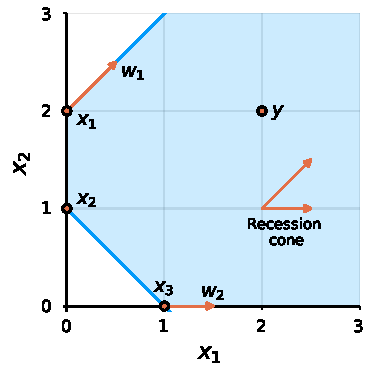
\includegraphics{chapters/chapter_12/figures/Figure1.pdf}
	\caption{Example showing that every point of $P = \braces{x_1 - x_2 \geq -2; x_1 + x_2 \geq 1, x_1,x_2 \geq 0}$ can be represented as a convex combination of its extreme point and a linear combination of its extreme rays} \label{p1c7:fig:resolution_example}
\end{figure}


\subsection{Dantzig-Wolfe decomposition}

We start with the Dantzig-Wolfe decomposition, which consists of an alternative approach for reducing memory requirements when solving large-scale linear programming problems. Then, we show how this can be expanded further with the notion of delayed variable generation to yield a truly decomposed problem.

As before, let $P_k = \braces{x_k \geq 0 : D_kx_k = d}$, with $P_k \neq \emptyset$ for $k \in \braces{1,\dots,K}$. Then, the problem $P$ can be reformulated as:
%
\begin{align*}
	\mini \ & \sum_{k = 1}^K c_k ^\top x_k 	\\
	\st & \sum_{k=1}^K A_k x_k = b \\
	& x_k \in P_k, \ \forall k \in \braces{1,\dots,K}. 
\end{align*}
%
Notice that $P$ has a complicating constraint structure, due to the constraints $\sum_{k=1}^K A_k x_k = b$. In order to devise a decomposition method for this setting, let us first assume that we have available for each of the sets $P_k$, $k \in \braces{1,\dots,K}$, (i) all extreme points, represented by $x_k^j$, $\forall j \in J_k$; and (ii) all extreme rays $w_k^r$, $\forall r \in R_k$. As one might suspect, this is in principle a demanding assumption, but one that we will be able to drop later on.

Using the Resolution theorem (Theorem \ref{p1c7:thm:resolution_theorem}), we know that any element of $P_k$ can be represented as 
%
\begin{equation} \label{p1c7:eq:resolution_representation}
	x_k = \sum_{j \in J_k} \lambda_k^j x_k^j + \sum_{r \in R_k} \theta_k^r w_k^r, 	
\end{equation}
%
where $\lambda_k^j \geq 0$, $\forall j \in J_k$, are the coefficients of the convex combination of extreme points, meaning that we also observe $\sum_{j \in J_k} \lambda_k^j = 1$, and $\theta_k^r \geq 0$, $\forall r \in R_k$, are the coefficients of the conic combination of the extreme rays.

Using the identity represented in \eqref{p1c7:eq:resolution_representation}, we can reformulate $P$ onto the \emph{main problem} $P_M$ as follows.
%
\begin{align} 
	(P_M) : \mini \ & \sum_{k =1}^K \left(\sum_{j \in J_k} \lambda_k^jc_k ^\top x^j_k   + \sum_{r \in R_k} \theta_{k}^rc_k^\top w_k^r \right)	\nonumber\\
	\st & \sum_{k = 1}^K \left(\sum_{j \in J_k}\lambda_k^j A_k x_k^j + \sum_{r \in R_k} \theta_k^r A_k w_k^r\right) = b \label{p1c7:eq:pm_const}\\
	& \sum_{j \in J_k}\lambda_k^j = 1, \ \forall k \in \braces{1, \dots, K} \label{p1c7:eq:cc_const}\\
	& \lambda_k^j \geq 0,  \theta_k^r \geq 0, \forall j \in J_k, r \in R_k, k \in \braces{1, \dots, K}. \nonumber 
\end{align}
%
Notice that \eqref{p1c7:eq:pm_const} and \eqref{p1c7:eq:cc_const} can be equivalently represented as
%
\begin{equation*}
	\sum_{k \in K}\left(\sum_{j \in J_k}\lambda_k^j \begin{bmatrix} A_kx_k^j \\ e_k\end{bmatrix} + \sum_{r \in R_k}\theta_k^r \begin{bmatrix} A_kw_k^r \\ 0\end{bmatrix}\right) = \begin{bmatrix} b \\ 1\end{bmatrix},
\end{equation*}
%	  	   
where $e_k$ is the unit vector (i.e., with 1 in the $k^\text{th}$ component, and $0$ otherwise). Notice that $P_M$ has as many variables as the number of extreme points and extreme rays of $P$, which is likely to be prohibitively large.

However, we can still solve it if we use a slightly modified version of the revised simplex method. To see that, let us consider that $b$ is a $m$-dimensional vector. Then, a basis for $P_M$ would be of size $m + K$, since we have the original $m$ constraints plus one for each convex combination (arising from each subproblem $k \in K$). This means that we are effectively working with $(m + K) \times (m + K)$ matrices, i.e., the basic matrix $B$ and its inverse $B^{-1}$. Another element we need is the vector of simplex multipliers $p$, which is a vector of dimension $(m + K)$.

The issue with the representation adopted in $P_M$ arises when we are required to calculate the reduced costs of \emph{all} the nonbasic variables, since this is the critical issue for its tractability. That is where the method provides a clever solution. To see that, notice that the vector $p$ is formed by components $p^\top = (q, r_1, \dots, r_K)^\top$, where $q$ represent the $m$ dual variables associated with \eqref{p1c7:eq:pm_const}, and $r_k$, $\forall k \in \braces{1,\dots,K}$, are the dual variables associated with \eqref{p1c7:eq:cc_const}. 

The reduced costs associated with the extreme-point variables $\lambda_k^j$, $j \in J_K$, is given by
%
\begin{equation}
	c_k^\top x_k^j - [q^\top ~ r_1 ~ \dots ~ r_K]	\begin{bmatrix} A_k x_k^j \\ e_k \end{bmatrix} = (c_k^\top - q^\top A_k)x_k^j - r_k.
\end{equation}
%
Analogously, the reduced cost associated with extreme-ray variables $\theta_k^r$, $r \in R_k$, is
\begin{equation}
	c_k^\top w_k^r - [q^\top ~ r_1 ~ \dots ~ r_K]	\begin{bmatrix} A_k w_k^r \\ 0 \end{bmatrix} = (c_k^\top - q^\top A_k)w_k^r.
\end{equation}
%
The main difference is how we assess the reduced costs of the non-basic variables. Instead of explicitly calculating the reduced costs of all variables, we instead rely on an optimisation-based approach to consider them only \emph{implicitly}. For that, we can use the subproblem 
%
\begin{align*}
	(S_k):  \mini_x \overline{c}_k = \ & (c_k^\top - q^\top A_k)x_k \\
	\st & x_k \in P_k,			
\end{align*} 
%
which can be solved in parallel for each subproblem $k \in \braces{1,\dots,K}$. The subproblem $S_k$ is known as the \emph{pricing problem}. For each subproblem $k = 1, \dots, K$, we have the following cases.

 We might observe that $\overline{c}_k = -\infty$. In this case, we have found an \emph{extreme ray} $w_k^r$ satisfying $(c_k^\top - q^\top A_k)w_k^r < 0$. Thus, the reduced cost of the associated extreme-ray variable $\theta_k^r$ is negative. 

If that is the case, we must generate the column
%
\begin{equation*}
	\begin{pmatrix}
		A_kw_k^r \\ 0
	\end{pmatrix}
\end{equation*}
%
associated with $\theta_k^r$ and make it enter the basis.		

Otherwise, being $S_k$ bounded, i.e., $\overline{c}_k < \infty$, two other cases can occur. The first is the case in which $\overline{c}_k < r_k$. Therefore, we found an extreme point $x_k^j$ satisfying $(c_k^\top - q^\top A_k)x_k^j - r_k < 0$. Thus, the reduced cost associated with the extreme-point variable $\lambda_k^j$ is negative and, analogously, we must generate the column
%
\begin{equation*}
	\begin{pmatrix}
		A_kx_k^j \\ e_k
	\end{pmatrix}
\end{equation*}
%
associated with $\lambda_k^j$ and make it enter the basis.

The last possible case is when we observe that $r_k < \overline{c}_k < \infty$. In this case, the pricing problem could not identify a beneficial variable to be made basic, and therefore there is not an extreme point or ray with negative reduced cost for subproblem $k$. If this condition holds for all $k = 1, dots, K$, then all necessary extreme points and rays to characterise the region where the optimal extreme point lies (or one of the extreme points, in the case of multiple solutions) have been found and the optimal solution can be recovered. 

Algorithm \ref{p1c7:alg:DW} summarises the Dantzig-Wolfe method. The two most remarkable features of the method are (i) the fact that columns are not explicitly represented, but generated ``on demand'' and (ii) the fact that the pricing problem requires the solution of another linear programming problem. Analogously to the simplex method, it might be necessary to employ a ``Phase 1'' approach to obtain an initial basis to start the algorithm.

\begin{algorithm}[h]
\caption{Dantzig-Wolfe decomposition} \label{p1c7:alg:DW}
\begin{algorithmic}[1] %line numbering frequency. 
	\State {\bf initialise.} 
	Let $B$ be a BFS for $P_M$ and set $l \gets 0$. 
	\Repeat 
	   \For {$k \in \braces{1,\dots,K}$} 
	        \State solve $S_k$ and let $\overline{c}_k = \min_x \braces{S_k}$
	        \If{$\overline{c}_k  = -\infty$} 
	        	\State obtain extreme ray $w_k^r$ and make $R_k^l = R_k^l \cup \braces{w_k^r}$.
	        	\State generate column $(A_kw_k^r, 0)$ to become basic.
	        \ElsIf {$\overline{c}_k < r_k < \infty$}
	        	\State obtain extreme point $x_k^j$ and make $J_k^l = J_k^l \cup \braces{x_k^j}$.
	        	\State generate column $(A_kx_k^j, e_k)$ to become basic.
	        \EndIf  
	    \EndFor
			\State select one of the generated columns to replace one of the columns of $B$ and update $B$ accordingly. 
	    \State $l \gets l + 1$.            	
		\Until{$\overline{c}_k  > r_k$ for all $k \in \braces{1,\dots,K}$} 
	\State {\bf return} $B$
\end{algorithmic}  
\end{algorithm}

Under a theoretical standpoint, the Dantzig-Wolfe method is equally efficient as the revised simplex method. There are however two settings where the decomposition is most favourable. The first, consists of applications in which the pricing problem can be solved in a closed-form, without invoking a method to solve an additional linear programming subproblem. There are a few examples in which this happens to be the case and certainly many others yet to be discovered.

Secondly, the memory requirements of the Dantzig-Wolfe decomposition makes it an interesting approach for very large-scale problems. The original simplex method requires an amount of memory space that is $O((m + K \times m_0)^2)$, where $m_0$ is the number of rows of $D_k$, for $\forall k \in \braces{1,\dots, K}$. This is essentially the size of the inverse basic matrix $B^{-1}$. In contrast, the Dantzig-Wolfe reformulation requires $O((m + K)^2) + K \times O(m_0^2)$ of memory space, with the first term referring to the main problem inverse basic matrix and the second to the pricing problems basic matrices. For example, for a problem in which $m = m_0$ and much larger than, say, $K=10$, this implies that the memory space required by the Dantzig-Wolfe reformulation is 100 times smaller, which can substantially enlarge the range of large-scale problems that can be solved for the same amount of computational resources available.


\subsection{Delayed column generation}
 
The term column generation can also refer to a related, and perhaps more widely known, variant of the Dantzig-Wolfe decomposition. In that, the main problem $P_M$ is also repeatedly solved, each time being incremented by an additional variable (or variables) associated with the column(s) identified with negative reduced costs in the pricing problem $S_k$, $k \in \braces{1,\dots,K}$. This is particularly useful for problems with exponentially increasing number of variables, or with a large number of variables associated with the complicating constraints (i.e., when $m$ is a large number).

\begin{algorithm}[h]
    \caption{Column generation algorithm} \label{p1c7:alg:CG}
    \begin{algorithmic}[1] %line numbering frequency. 
    \State {\bf initialise.} 
    Let $\tilde{X}_k \subset X_k$, for $k \in \braces{1,\dots,K}$, and set
    $l \gets 0$. 
    	\Repeat \label{Alg2:loop}
        \State solve $P_M^l$ to obtain $\lambda^{*l} = (\lambda_1^{*l},\dots, \lambda_K^{*l})$ and duals $(q^{*l}, \braces{r_k^{*l}}_{k=1}^K)$.
        \For {$k \in \braces{1,\dots,K}$} 
            \State solve the pricing problem
            $$\overline{x}^{*l}_k \gets \argmin \braces{c_k^\top x_k - q^{*l}(A_kx_k) - r^{*l}_k : x_k \in P_k}.
            $$
            \If{$\overline{c}_k = c_k^\top \overline{x}^{*l}_k - q^{*l}(A_k\overline{x}^{*l}_k) < r^{*l}_k$} $\tilde{X}_k \gets \tilde{X}_k \cup \braces{\overline{x}^{*l}_k}$ \label{p1c7:alg:CGcolgen}
            \EndIf  
        \EndFor
        \State $l \gets l + 1$.
    	\Until{$\overline{c}_k  > r_k$ for all $k \in \braces{1,\dots,K}$} 
    \State {\bf return} $\lambda^{*l}$.
    \end{algorithmic}
\end{algorithm}

The (delayed) column generation method is presented in Algorithm \ref{p1c7:alg:CG}. Notice in Line \ref{p1c7:alg:CGcolgen} the step that is generating new columns in the main problem $P_M$, represented in the statement $\tilde{X}_k \gets \tilde{X}_k \cup \braces{\overline{x}^{*l}_k}$. That is precisely when new variables $\lambda_k^{t}$ are introduced in the $P_M$ with coefficients represented by the column
%
\begin{equation*}
	\begin{pmatrix}
            c_k\overline{x}_k^{*l}\\
            A_k\overline{x}_k^{*l}\\
            e_k
    \end{pmatrix}.
\end{equation*}

Notice that the unbounded case is not treated to simplify the pseudocode, but could be trivially adapted to return extreme rays to be used in $P_M$, like the previous variant presented in Algorithm \ref{p1c7:alg:DW}. Also, notice that the method is assumed to be initialised with a collection of columns (i.e., extreme points) $\tilde{X}_k$, which can normally be obtained from inspection or using a heuristic method.

We finalise showing that the Dantzig-Wolfe and column generation methods can provide information related to its own convergence. This means that we have access to an optimality bound that can be used to monitor the convergence of the method and allow for a preemptive termination given an acceptable tolerance. This bounding property is stated in Theorem \ref{p1c7:thm:CG_bound}.

\begin{theorem} \label{p1c7:thm:CG_bound}
	Suppose $P$ is feasible with finite optimal value $z$. Let $\overline{z}$ be the optimal cost associated with $P_M$ at a given iteration $l$ of the Dantzig-Wolfe method. Also, let $r_k$ be the dual variable associated with the convex combination of the $k^\text{th}$ subproblem and $z_k$ its optimal cost. Then
		%
		\begin{equation*}
			z + \sum_{k=1}^K (z_k - r_k) \leq z \leq \overline{z}.	
		\end{equation*}
\end{theorem}

\begin{proof}
	
	We know that $z \leq \overline{z}$, because a solution for $P_M$ is primal feasible and thus feasible for $P$.
	
	Now, consider the dual of $P_M$
	%
	\begin{align*}
		(D_M): ~\maxi \ & q^\top b + \sum_{k=1}^K r_k \\
		\st & q^\top A_k x_k^j + r_k \leq c_k^\top x_k^j, \ \forall j \in J_k, \forall k \in \braces{1,\dots, K} \\
		& q^\top A_kw_k^r \leq c_k^\top w_k^r, \ \forall r \in R_k, \forall k \in \braces{1,\dots, K} \\ 
	\end{align*}
	%
	We know that strong duality holds, and thus $z = q^\top b + \sum_{k=1}^K r_k $ for dual variables $(q, r_1, \dots, r_K)$. 
	
	Now, since $z_k$ are finite, we have $\min_{j \in J_k}(c_k^\top x_k^j - q^\top A_k x_k^j) = z_k$ and $\min_{r \in R_k}(c_k^\top w_k^r - q^\top D_k w_k^r) \geq 0$, meaning that $(q, z_1, \dots, z_K)$ is feasible to $D_M$. By weak duality, we have that
	%
	\begin{equation*}
		z \geq q^\top b + \sum_{k=1}^K	z_k = q^\top b + \sum_{k=1}^K r_k + \sum_{k=1}^K (z_k - r_k) = z + \sum_{k=1}^K (z_k - r_k). \qedhere	
	\end{equation*}
\end{proof}


\section{Benders decomposition}

Benders decomposition is an alternative decomposition method, suitable for settings in which \emph{complicating variables} are present. Differently than the Dantzig-Wolfe decomposition, the method presumes from the get-go the employment of delayed constraint generation. 

Benders decomposition has made significant inroads into practical applications. Not only is it extensively used in problems related to multi-period decision-making under uncertainty, but it is also available in the commercial solver CPLEX to be used directly, only requiring the user to indicate (or annotate) which are the complicating variables. 


\subsection{Parametric optimisation problems} \label{section_731}

Before we proceed, let us develop the idea of having optimisation problems stated as functions of the input data. Specifically, let 
%
\begin{equation*}
	P(b) = \braces{x \in \reals^n : Ax = b, x \geq 0}
\end{equation*}
%
be defined as a function of the input vector $b \in \reals^m$. That is, $P(b)$ is the set of feasible solutions when the right-hand side is set to $b$. Then, let $S = \braces{b \in \reals^m : P(b) \neq \emptyset}$ be the set of all vectors $b$ for which $P$ has at least one feasible solution. Being so, we can restate the set $S$ as 
%
\begin{equation*}
	S = \braces{Ax : x \ge 0}.
\end{equation*}
%
That is, the set $S$ is formed by the conic combination of the columns of $A$ for which $x$ is nonnegative (or, in other words, that $P(b)$ is feasible). Also, notice that this is a convex set, as discussed in Section \ref{section_621}. For any $b \in S$, we can define the function
%
\begin{equation}
	F(b) = \min_x \braces{c^\top x : x  \in P(b)},	
\end{equation}
%
which takes as an argument $b$ and returns the optimal value of the parametrised optimisation problem. Notice that evaluating $F$ requires that an optimisation problem is solved.

Now, let us assume that the dual feasibility set 
%
\begin{equation*}
	S_D = \braces{p \in \reals^m : p^\top A \le c}	
\end{equation*}
% 
is not empty. That implies that $F(b)$ is finite for every $b \in S$ since different $b$'s simply imply that different objective functions $p^\top b$ over $S_D$ are considered. Our main objective here is to understand the structure of the function $F: S \to \reals$. 

Let $\overline{b} \in S$ be a particular $b$. Suppose that there exists a nondegenerate optimal BFS $x_B$ with basis $B$. Then, we have that $x_B = B^{-1}\overline{b}$, $F(\overline{b}) = c_B^\top x_B =  c_B^\top B^{-1}\overline{b}$ and that all reduced costs are nonnegative. 

Now, if we change $\overline{b}$ to $b$ such that the difference is sufficiently small, $B^{-1}\overline{b}$ remains positive and, consequently, $x_B$ remains a basic feasible solution. Furthermore, since $b$ does not affect the reduced costs (recall that our optimality condition is given by $\overline{c} = c^\top - c_B ^\top B^{-1}A \ge 0$), they remain nonnegative. Notice that this is the same argument we used in Section \ref{section_613} when we discussed changes in the input data in the context of sensitivity analysis.

The optimal value $F(b)$ associated with this new $b$ sufficiently close to $\overline{b}$   
%
\begin{equation*}
	F(b) - F(\overline{b})= c_B B^{-1}(b - \overline{b}) = p^\top (b - \overline{b}) 
\end{equation*}
%
where $p = c_B B^{-1}$ is the optimal solution of the dual problem 
%
\begin{align*}
	\maxi & p^\top b \\
	\st   & p^\top A \le c.
\end{align*}
%
This allows us to observe two important characteristics of $F$. First, in the vicinity of $\overline{b}$, $F(b)$ is a linear function of $b$, Also, $p$ represents a \emph{gradient} of $F$. This, again, is an alternative view to the conclusions we drew earlier in Section \ref{section_613}, and, in a way, further strengthens the idea of the optimal dual variables $p$ representing marginal values regarding changes in the components of $b$.

With the above, we can formalise an important result regarding the convexity of the function $F(b)$.

\begin{theorem}[Convexity of $F(b)$]
	The optimal value function $F(b)$ is convex in $b$ on the set $S$.
\end{theorem}

\begin{proof}

	Let $b^i \in S$ and $x^i$ be their associated optimal solution, for $i = 1,2$. Thus, $F(b^i) = c^\top x^i$, for $i=1,2$. Let $\lambda \in [0,1]$. The vector $\overline{x} = \lambda x^1 + (1-\lambda)x^2$ is nonnegative, and $A\overline{x} = \lambda b^1 + (1-\lambda)b^2$. Thus, $\overline{x}$ is a feasible solution when $b$ is set to $\lambda b^1 + (1-\lambda)b^2$. Therefore,
	%
	\begin{equation*}
		F(\lambda b^1 + (1-\lambda)b^2) \le c^\top \overline{x}	= \lambda c^\top x^1 + (1-\lambda) c^\top x^2 = \lambda F(b^1) + (1-\lambda) F(b^2),
	\end{equation*}
	%
	which is the definition of a convex function. The first inequality is valid because $\overline{x}$ is a feasible solution for when $b$ is set to $\lambda b^1 + (1-\lambda)b^2$.
\end{proof}


\subsection{Properties of the optimal value function $F(b)$} \label{section_732}

Let us again consider the dual problem $D$
%
\begin{align*}
	D: \maxi & p^\top b \\
	\st   & p^\top A \le c,
\end{align*}
%
which is again assumed to be feasible. For any $b$ in $S$, $F(b)$ is finite, and by strong duality (cf. Theorem \ref{p1c5:thm:strong_duality}), we have that $F(b) = p^\top b$. Because of our outstanding assumption that $A$ has $m$ linearly independent rows (and therefore, $m$ linearly independent columns), Theorem \ref{p1c3:thm:exist_extreme_point} guarantees that the feasible region of $D$ has at least one extreme point.

Let us suppose that we know all the extreme points $p^1, \dots, p^K$ of $D$. As the optimal solution for $D$ must be an extreme point, we can redefine $F$ as
%
\begin{equation} \label{p1c7:eq:function_F}
	F(b) = \max_{i = 1, \dots, K} (p^i)^\top b, \forall b \in S.
\end{equation}
%
Specifically, $F$ is the maximum of a finite collection of linear functions, and thus, piecewise linear. Furthermore, within the region where $F(b)$ is linear, or, as we have seen before, the change in $b$ is such that the corresponding optimal basis $B$ of the primal does not change, $F(b) = (p^i)^\top b$ where $p^i$ is the corresponding dual cost.

Finally, we must consider the lack of differentiability of $F$. Notice that specific values of $b$ will indicate the point at which the optimal basis $B$ changes, which implies a change in $p$. These ``junctions'' represent the points in which $D$ has multiple (i.e., not unique) solutions, which, as we have also seen, implies that the primal problem becomes degenerate.

Let us assume that we change $b$ in a particular way, i.e., $b = \overline{b} + \theta d$, where $\theta \in \reals$. We can then redefine $F$ by letting 
%
\begin{equation*}
	f(\theta) = F(\overline{b} + \theta d).
\end{equation*}
%
From \eqref{p1c7:eq:function_F}, we obtain
%
\begin{equation*}
	f(\theta) = \max_{i = 1, \dots, K} (p^i)^\top (\overline{b} - \theta d), \overline{b} + \theta d \in S
\end{equation*}
%
which represents the optimal cost as a function of the scalar $\theta$. In fact, $f(\theta)$ represents a section of the function $F$ in the direction given by the vector $d$, which is thus also piecewise linear and convex (and can be plotted). Figure \ref{p1c7:fig:b_function_theta} illustrates the function $f$ projected onto direction $d$ as a function of $\theta$.

\begin{figure}
	\begin{tikzpicture}
		\node (pic) at (0,0) {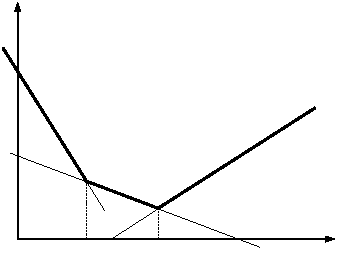
\includegraphics{chapters/chapter_12/figures/Figure2.pdf}};
		\node[right] (p1) at (-1.75,-0.25) {$(p^1)^\top (\overline{b} + \theta d)$};
		\node[right] (p2) at (0.5, -1.5) {$(p^2)^\top (\overline{b} + \theta d)$};
		\node[right] (p3) at (1.25,-0.6) {$(p^3)^\top (\overline{b} + \theta d)$};
		\node[below] (theta1) at (-1.4, -1.9) {$\theta_1$};
		\node[below] (theta2) at (-0.125, -1.9) {$\theta_2$};
		\node[below] (theta) at (2.7, -1.9) {$\theta$};
		\node[right] (f_theta) at (-2.5, 2) {$f(\theta)$};
	\end{tikzpicture}	
	\caption{The optimal cost function $F$ as a function of $b$ in the direction $d$. The feasibility set $S_D$ has three extreme points $p^1$, $p^2$, and $p_3$, each associated with a hyperplane $(p^i)^\top(\overline{b} + \theta d)$} \label{p1c7:fig:b_function_theta}
\end{figure}

To finalise, we return to one remaining issue associated with differentiability. Although $p$ can be seen as a gradient of $F(b)$ at $b$, we know that $F$ is not differentiable everywhere. To circumvent that, we require a generalisation of the the concept of gradients, which is given by the notion of subgradients. 

\begin{definition}
	Let $F$ be a convex function on the convex set $S$. Let $\overline{b} \in S$ The vector $p$ is a subgradient of of $F$ at $\overline{b}$ if
	\begin{equation}
		F(\overline{b}) + p^\top (b - \overline{b}) \le F(b), \forall b \in S.
	\end{equation}
\end{definition}

Figure \ref{p1c7:fig:b_function} illustrates the notion of a subgradient. Notice that, in general, the subgradient is a singleton, composed only of the gradient (or normal vector) of the hyperplane, which is given by the vector $p$. At the nondifferentiable points (the junctions), the subgradient comprises all hyperplanes defined between the two hyperplanes intersecting (or all nonnegative linear combinations of the normal vectors of the intersecting hyperplanes). For these values of $b$, we notice that the dual problem has multiple solutions, implying that the referring BFS to the primal problem is denegerate.   


The last result we need is to show that the optimal solution of the dual problem $p^*$ is in fact a subgradient of $F(\overline{b})$ at $\overline{b}$.

\begin{theorem}
	Suppose that the linear programming problem $P = \mini \braces{c^\top x : Ax = \overline{b}, x \ge 0}$ is feasible and the optimal cost is finite. Then, a vector $p \in \reals^m$ is an optimal solution to the dual problem if and only if it is a subgradient of the optimal value function $F$ at $\overline{b}$.
\end{theorem}

\begin{proof}
	Recall that $F$ is defined on the set $S = \braces{b \in \reals^m : P(b) \neq \emptyset}$, and that $P(b) = \braces{x \in \reals^n : Ax = b, x \geq 0}$. Suppose $p$ is an optimal solution to the dual problem $D$. Then, strong duality implies that $p^\top \overline{b} = F(\overline{b})$. Consider now an arbitrary $b \in S$. For any feasible solution $x \in P(b)$, we have from weak duality that 
	\begin{equation*}
		p^\top b \le c^\top x \Rightarrow p^\top b \le \min_{x \in P(b)} c^\top x = F(b).
	\end{equation*}
	Notice that this implies that $p^\top b - p^\top \overline{b} \le F(b) - F(\overline{b})$, which in turn yields that $p$ is a subgradient of $F$ at $\overline{b}$ since it rearranges to
	\begin{equation*}
		F(\overline{b}) + p^\top (b - \overline{b}) \le F(b).
	\end{equation*}
	Let us consider the converse. Assume that $p$ is a subgradient of $F$ at $\overline{b}$. Thus, we have 
	\begin{equation}
		F(\overline{b}) + p^\top (b - \overline{b}) \le F(b), \ \forall b \in S. \label{p1c7:eq:subgradient_proof}
	\end{equation}
	Let choose an $x \ge 0$, and let $b = Ax$, meaning that $x \in P(b)$ and that $F(b) \le c^\top x$. Using \eqref{p1c7:eq:subgradient_proof}, we obtain
	\begin{equation*}
		p^\top Ax = p^\top b \le F(b) - F(\overline{b}) + p^\top \overline{b} \le c^\top x - F(\overline{b}) + p^\top \overline{b}.
	\end{equation*}
	Since $x \ge 0$, this implies that $p^\top A \le c$, showing that $p$ is a dual feasible solution. Also, for $x = 0$, we obtain $F(\overline{b}) \le p^\top \overline{b}$. Now, using weak duality, we have that a dual feasible solution $p'$ satisfies $(p')^\top \overline{b} \le F(\overline{b})$. Combining the two, we show that $p$ is dual optimal, since
	\begin{equation*}
		(p')^\top \overline{b} \le  p^\top \overline{b}.
	\end{equation*}
\end{proof}

\begin{figure}[h]
	\begin{tikzpicture}
		\node (pic) at (0,0) {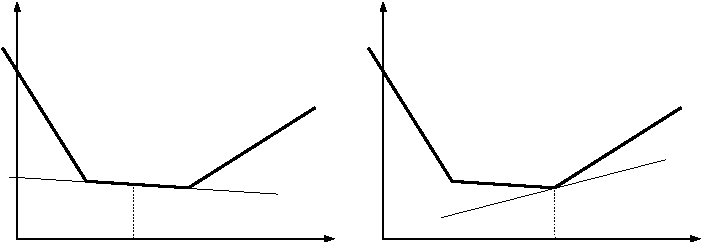
\includegraphics{chapters/chapter_12/figures/Figure3.pdf}};
		\node[right] (Fb1) at (-3,-1.5) {$F(\overline{b}) + p^\top(b - \overline{b})$};
		\node[right] (Fb2) at (4.6,-1) {$F(\overline{b}) + p^\top(b - \overline{b})$};
		\node[below] (b1) at (-3.7, -2) {$\overline{b}$};
		\node[below] (b2) at (3.4, -2) {$\overline{b}$};
		\node[below] (b_axis1) at (-0.3, -2) {$b$};
		\node[below] (b_axis2) at (5.9, -2) {$b$};
		\node[right] (Fb_axis1) at (-5.65, 2) {$F(b)$};
		\node[right] (Fb_axis1) at (0.55, 2) {$F(b)$};
	\end{tikzpicture}	
	\caption{The subgradients of the function $F$ at $\overline{b}$. On the left, the unique subgradient of $F$ at $\overline{b}$ is the gradient of the affine function $F(\overline{b}) + p^\top(b - \overline{b})$. On the right, the gradient of the affine function $F(\overline{b}) + p^\top(b - \overline{b})$ at $\overline{b}$ is contained in a subgradient for $F$ at $\overline{b}$.} \label{p1c7:fig:b_function}
\end{figure}



Therefore, more generally, we can say that at the breakpoints, $F$ has multiple subgradients while everywhere else, the subgradients are unique and correspond to the gradients of $F$.


\subsection{Benders decomposition}

Let us now return to the Benders decomposition method. Once again, let the problem $P$ be defined as
%
\begin{align*}
	(P) :\mini_{x,y} & c^\top x + \sum_{k=1}^K f_k^\top y_k \\
		  			 & Ax = b \\
		  			 & C_k x + D_k y_k = e_k, \ k \in \braces{1, \dots, K} \\
		  			 & x \geq 0, y_k \geq 0, \ k \in \braces{1,\dots, K}. 
\end{align*}
%
Notice that this is equivalent to the problem $P'$ presented in Section \ref{section_71}, but with a notation modified to make it easier to track how the terms are separated in the process. We can see that $P$ has a set of complicating variables $x$, which becomes obvious when we recast the problem as
%
\begin{center}
	\begin{tabular}{cccccccccc}
		 $c^\top x$ & + & $f_1^\top y_1$ & + & $f_2^\top y_2$ & + & $\dots$ & + & $f_k^\top y_k$  &  \\
	 	 $Ax$       &   &                &   &                &   &         &   &                 & = $b$ \\
		 $C_1 x$    & + & $D_1 y_1$      &   &                &   &         &   &                 & = $e_1$  \\
		 $C_2 x$    &   &                & + & $D_2 y_2$      &   &         &   &                 & = $e_2$    \\
		 $\vdots$   &   &  $\vdots$      &   &                &   & $\ddots$&   &                 &  $\vdots$   \\
		 $C_K x$    &   &                &   &                &   &         & + & $D_k y_k$       & = $e_K$  \\
		 $x$        &   & $y_1$          &   &  $y_2$         &   & $\dots$ &   & $y_k$           & $\geq 0$  
	\end{tabular}	
\end{center}
 
This structure is sometimes referred to as block-angular, referring to the initial block of columns on the left (as many as there are components in $x$) and the diagonal structure representing the elements associated with the variables $y$. In this case, notice that if the variable $x$ were to be removed, or fixed to a value $x = \overline{x}$, the problem becomes separable in $K$ independent parts
% 
\begin{align*} 
	(S_k) : \mini_y & f_k^\top y_k \\
	\st & D_ky_k = e_k - C_k \overline{x} \\
	& y_k \geq 0.
\end{align*}
%
Notice that these subproblems $k \in \braces{1,\dots, K}$ can be solved in parallel and, in certain contexts, might even have analytical closed-form solutions. The part missing is the development of a coordination mechanism that would allow for iteratively updating the solution $\overline{x}$ based on information emerging from the solution of the subproblems $k \in \braces{1,\dots, K}$.

To see how that can be achieved, let us reformulate $P$ as 
%
\begin{align*}
	(P_R) : \mini_x & c^\top x + \sum_{k=1}^K z_k(x) \\
	\st   & Ax = b \\
	      & x \geq 0.
\end{align*}
%
where, for $k \in \braces{1,\dots, K}$,  
%
\begin{equation*}
	z_k(x) = \mini_y \braces{f_k^\top y_k : D_ky_k = e_k - C_k x}.	
\end{equation*}
%
Notice the resemblance between $z_k(x)$ and the optimal value function $F(b)$ introduced in Section \ref{section_731}. This is because the subproblems become parametric optimisation problems but as a function of $x$. That is, in this case, the subproblems are assumed to have $x = \overline{x}$ set as a parameter. Analogously, evaluating $z_k(x)$ requires solving the subproblem $S_k$, which, in turn, depends on $x$. 

The Benders decomposition works by iteratively constructing the optimal value function. Instead of assuming that all dual extreme points are known, we collect them iteratively, forming an approximation of the optimal value function $z_k(x)$ that becomes increasingly precise as we collect more such extreme points. And, to find new dual extreme points, we can use our current approximation of the optimal value function $z_k(x)$ in $P_R$, which, once solved, returns us a new $\overline{x}$ to be used for finding a new dual extreme point. Notice that this procedure is akin to iteratively finding the linear segments that form the optimal value functions $z_k(x)$.

To formalise the discussion above, let us first consider the dual formulation of the subproblems $k \in \braces{1,\dots, K}$, which is given by
%
\begin{align*}
	(S^D_k): z^D_k = \maxi \ & p_k^\top (e_k - C_k x) \\
	\st   & p_k^\top D_k \leq f_k.	 
\end{align*}
%
%The main advantage of utilising the equivalent dual formulation is to ``move'' the original decision variable $x$ to the objective function, a trick that will present its benefits shortly. 
Next, let us denote the feasibility set of $S^D_k$ as 
%
\begin{equation}
	P_k =\braces{p : p^\top D_k \leq f_k}, \forall k \in \braces{1,\dots,K}, 
\end{equation}
%
and assume that each $P_k \neq \emptyset$ with at least one extreme point\footnote{We have discussed in Section \ref{section_732} why we can assume that $P_k$ has at least one extreme point}. Relying on the resolution theorem (Theorem \ref{p1c7:thm:resolution_theorem}), we know that $P_k$ can be represented by its extreme points $p_k^i$, $i \in I_k$ and extreme rays $w^r_k$, $r \in R_k$.

As we assume that $P_k \neq \emptyset$, two cases can occur when we solve $S^D_k$, $k \in \braces{1,\dots, K}$. Either $S^D_k$ is unbounded, meaning that the relative primal subproblem is infeasible, or $S^D_k$ is bounded, meaning that $z^D_k < \infty$.

From the first case, we can use Theorem \ref{p1c6:thm:unb_polyhedra} to conclude that primal feasibility (or a bounded dual value $z^D_k < \infty$) can only be attained if and only if
%
\begin{equation}
	(w^r_k)^\top (e_k - C_k x) \leq 0, \ \forall r \in R_k. \label{p1c7:eq:feas_cut_all}	
\end{equation}
%
Furthermore, we know that if $S^D_k$ has a solution, that must lie on a vertex of $P_k$. So, having  available the set of all extreme vertices $p_k^i$, $i \in I_k$, we have that if one can solve $S^D_k$, it can be equivalently represented as
%
\begin{equation} \label{p1c7:eq:optimal_value_function_z}
	(S^D_k) : z_k(x) = \max_{i \in I_k}~ (p^i_k)^\top (e_k - C_k x),
\end{equation}   
%
which can be equivalently reformulated as
\begin{align}
	\mini \ & \theta_k \label{p1c7:eq:opt_cut_all1} \\
	\st & \theta_k \geq (p^i_k)^\top (e_k - C_k x), \ \forall i \in I_k. \label{p1c7:eq:opt_cut_all2}
\end{align}

Again, notice that \eqref{p1c7:eq:optimal_value_function_z} is equivalent to \eqref{p1c7:eq:function_F}. Combining \eqref{p1c7:eq:feas_cut_all}--\eqref{p1c7:eq:opt_cut_all2}, we can reformulate $P_R$ into a single-level equivalent form 
%
\begin{align}
	(P_R) : & \mini_x c^\top x + \sum_{k=1}^K\theta_k \nonumber\\
	\st   & Ax = b \nonumber \\
		  & (p^i_k)^\top (e_k - C_k x) \leq  \theta_k, \ \forall i \in I_k, \forall k \in \braces{1,\dots, K}  \label{p1c7:eq:opt_cut} \\
		  & 	(w^r_k)^\top (e_k - C_k x) \leq 0, \ \forall r \in R_k, \forall k \in \braces{1, \dots, K} \label{p1c7:eq:feas_cut} \\
	      & x \geq 0. \nonumber
\end{align}
%
Notice that, just like the reformulation used for the Dantzig-Wolfe method presented in Section \ref{section_72}, the formulation of $P_R$ is of little practical use since it requires the complete enumeration of (a typically prohibitive) number of extreme points and rays and is likely to be computationally intractable due to the large number of associated constraints. To address this issue, we can employ delayed constraint generation and iteratively generate only the constraints we observe to be violated. Notice that this can be alternatively interpreted as the idea of iteratively generating the segments of the optimal value function $z_k(x)$.

Following this idea, at a given iteration $l$, we have at hand a \emph{relaxed main problem} $P_M^l$, which comprises only some of the constraints associated with the dual extreme points and rays obtained until iteration $l$. The relaxed main problem can be stated as
%
\begin{align*}
	(P^l_M) : z_{P_M}^l = \mini_x & c^\top x + \sum_{k=1}^K\theta_k \\
	\st   & Ax = b \nonumber \\
		  & (p^i_k)^\top (e_k - C_k x) \leq  \theta_k, \ \forall i \in I_k^l, \forall k \in \braces{1, \dots, K}  \\
		  & (w^r_k)^\top (e_k - C_k x) \leq 0, \ \forall r \in R_k^l, \forall k \in \braces{1, \dots, K}  \\
	      & x \geq 0, 
\end{align*}
%
where $I_k^l \subseteq I_k$, $\forall k \in \braces{1,\dots,K}$ represent subsets of extreme points $p^i_k$ of $P_k$, and $R^l_k \subseteq R_k$ subsets of extreme rays $w^r_k$ of $P_k$.

We can iteratively obtain these extreme points and rays from the subproblems $S_k$, $k \in \braces{1, \dots, K}$. To see that, let us first define that, at iteration $l$, we solve the main problem $P_M^l$ and obtain a solution
%
\begin{equation*}
	\argmin_{x, \theta} \braces{P_M^l} = (\overline{x}^l, \overline{\theta}^l_1, \dots \overline{\theta}^l_K). 
\end{equation*}
%
We can then solve the subproblems $S_k^l$, $k \in \braces{1, \dots, K}$, for that fixed solution $\overline{x}^l$ and then observe if we can find additional constraints that were to be violated if they had been in the relaxed main problem in the first place. In other words, we can identify if the solution $\overline{x}^l$ allows for identifying additional extreme points $p^i_k$ or extreme rays $w^r_k$ of $P_k$ that were not yet included in $P_M^l$. 

Another way to interpret this notion of violation is to again think of the optimal value function. When we solve $S_k^l$, for each $k \in \braces{1, \dots, K}$, we are obtaining a ``true`` (as opposed to approximate) evaluation of the optimal value function $z_k(\overline{x}^l)$ which, when compared against the working approximation of $z_k$ (valued as $\theta_k$) in the main problem, provides a value that is greater than that of $\theta_k$, that is,
%
\begin{equation}
	\theta_k < (p^i_k)^\top (e_k - C_k \overline{x}^l).
\end{equation}
%
This implies that the approximation of the optimal value function has a segment missing at $\overline{x}^l$, which is precisely the one given by $(p^i_k)^\top (e_k - C_k x)$. 

Figure \ref{p1c7:fig:benders_iteration} illustrates how the optimal value function approximation is iteratively constructed.

\begin{figure}[h]
	\begin{tikzpicture}
		\node (pic) at (0,0) {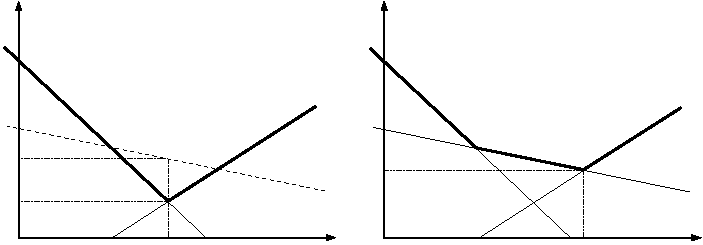
\includegraphics{chapters/chapter_12/figures/Figure4.pdf}};
		\node[right] (zb1_left) at (-5.4, 1) {$(p_k^1)^\top(e_k - C_kx)$};
		\node[left]  (zb2_left) at (0, 0.5) {$(p_k^2)^\top(e_k - C_kx)$};
		\node[right] (zb1_right) at (0.8, 1) {$(p_k^1)^\top(e_k - C_kx)$};
		\node[left]  (zb2_right) at (6.2, 0.5) {$(p_k^2)^\top(e_k - C_kx)$};
		\node[right] (zb3_right) at (4, -1.5) {$(p_k^3)^\top(e_k - C_kx)$};
		\node[right] (zb_opt) at (-2.6, -1.4) {$(p_k^*)^\top(e_k - C_kx)$};
		\node[below] (x1) at (-3.1, -1.9) {$\overline{x}^3$};
		\node[below] (x2) at (3.95, -1.9) {$\overline{x}^4$};
		\node[left]  (theta1) at (-5.6, -1.3) {$\overline{\theta}^3$};
		\node[left]  (theta2) at (0.6, -0.8) {$\overline{\theta}^4$};
		\node[left]  (z_dual) at (-5.6, -0.6) {$z(\overline{x}^3)$};
		\node[below] (x_axis1) at (-0.4, -2) {$x$};
		\node[below] (x_axis2) at (5.8, -2) {$x$};
		\node[right] (z_axis1) at (-5.6, 2) {$z_k(x)$};
		\node[right] (z_axis2) at (0.6, 2) {$z_k(x)$};
	\end{tikzpicture}	
	\caption{$z_k(x)$ is described by 3 line segments. At iteration $l=3$, two are available. The solution to $P_M^3$ returns $\overline{\theta}^3$, which is lower than $z(\overline{x}^3)$, obtained solving $S_k^D$ for $\overline{x}^l$. The solution $p^*_k = p^3_k$ from $z(\overline{x}^l)$ defines the missing segment $(p^*_k)^\top(e_k - C_kx)$. A new optimality cut is added and in iteration $l=4$, $\overline{x}^4$ is obtained from solving $P_M^4$. Notice that we would have $\overline{\theta}^{4} = z(\overline{x}^{4})$, meaning that the algorithm terminates.} \label{p1c7:fig:benders_iteration}
\end{figure}

To identify those violated constraints, first recall that the subproblem (in its primal form) is given by
%
\begin{align*}
	(S_k^l): \mini \ & f^\top y \\
	\st & D_k y_k = e_k - C_k \overline{x}^l \\
	& y_k \geq 0.
\end{align*}
%
Then, two cases can lead to generating violated constraints that must be added to the relaxed primal problem to form $P_M^{l+1}$. The first is when $S_k^l$ is feasible. In that case, a dual optimal basic feasible solution $p^{il}_{k}$ is obtained. If $(p^{il}_k)^\top(e_k - C_k \overline{x}^l) > \overline{\theta}_k^l$, then we can conclude that we just formed a violated constraint of the form of \eqref{p1c7:eq:opt_cut}. The second case is when $S_k^l$ is infeasible, then an extreme ray $w^{rl}_k$ of $P_k$ is available, such that $(w^{rl}_k)^\top(e_k - C_k \overline{x}^l) > 0$, violating \eqref{p1c7:eq:feas_cut}. 

Notice that the above can also be accomplished by solving the dual subproblems $S^D_k$, $k \in \braces{1, \dots, K}$, instead. In that case, the extreme point $p^{il}_k$ is immediately available and so are the extreme rays $w^{rl}_k$ in case of unboundedness.

Algorithm \ref{p1c7:alg:benders} presents a pseudocode for the Benders decomposition. Notice that the method can benefit in terms of efficiency from the use of dual simplex, since we are iteratively adding violated constraints to the relaxed main problem $P_M^l$. Likewise, the dual of the subproblem $S_k^l$, $S_k^{Dl}$ has only the objective function coefficients being modified at each iteration and, in light of the discussion in Section \ref{section_613}, can also benefit from the use of dual simplex. Furthermore, the loop represented by Line \ref{p1c7:alg:benders-loop} can be parallelised to provide further computational performance improvements. 

\begin{algorithm}[H]
    \caption{Benders decomposition} \label{p1c7:alg:benders}
    \begin{algorithmic}[1] %line numbering frequency. 
    \State {\bf initialise.} 
    Let $P_i^l = W_j^l = \emptyset$, for $k \in \braces{1,\dots,K}$, and set
    $l \gets 0$. 
    \Repeat 
        \State solve $P_M^l$ to obtain $\left(\overline{x}^l, \braces{\overline{\theta}_k^l}_{k=1}^K\right)$. 
        \For {$k \in \braces{1,\dots,K}$} \label{p1c7:alg:benders-loop}
            \State solve $S_k^{Dl}$.
            \If{$S_k^{Dl}$ is unbounded} 
            	\State obtain extreme ray $w_j^k$ and make $W^l = W^l \cup \braces{w_j^k}$.
            \Else
            	\State obtain extreme point $p_i^k$ and $P^l = P^l \cup \braces{p_i^k}$
            \EndIf  
        \EndFor
 
        \State $l = l + 1$.        	
    	\Until{$(p^i_k)^\top(e_k - C_k \overline{x}) \leq \overline{\theta}_k, \ \forall k \in \braces{1,\dots,K}$} 
    \State {\bf return} $\left(\overline{x}^l, \braces{\overline{\theta}_k^l}_{k=1}^K\right)$
  \end{algorithmic}
\end{algorithm}

Notice that the algorithm terminates if no violated constraint is found. This in practice implies that $(p^i_k)^\top(e_k - C_k \overline{x}) \leq \overline{\theta}_k$ for all $k \in \braces{1,\dots,K}$, and thus $(\overline{x}, \braces{\overline{\theta}_k}_{k=1}^K)$ is optimal for $P$. In a way, if one considers the dual version subproblem, $S_k^D$, one can notice that it is acting as an implicit search for values of $p^i_k$ that can make $(p^i_k)^\top(e_k - C_k \overline{x})$ larger than $\overline{\theta}_k$, meaning that the current solution $\overline{x}$ violates \eqref{p1c7:eq:opt_cut} and is thus not feasible to $P_M^l$. 

Also, every time one solves $P_M^l$, a dual (lower for minimisation) bound $LB^l = z_{P_M}^l$ is obtained. This is simply because the relaxed main problem is a relaxation of the problem $P$, i.e., it contains less constraints than the original problem $P$. A primal (upper) bound can also be calculated at every iteration, which allows for keeping track of the progress of the algorithm in terms of convergence and preemptively terminate it at any arbitrary optimality tolerance. That can be achieved by setting
%
\begin{align*}
	UB^l &= \min\braces{UB^{l-1}, c^\top \overline{x}^l + \sum_{k=1}^K f^\top \overline{y}_k^l} \\	
	&= \min\braces{UB^{l-1}, z_{P_M}^l - \sum_{k=1}^K \overline{\theta}_k^l + \sum_{k=1}^K z^{Dl}_{k}},
\end{align*}
%
where $(\overline{x}^l, \braces{\overline{\theta}^{l}_k}_{k=1}^K) = \argmin_{x, \theta} \braces{P_M^l}$, $\overline{y}_k^l = \argmin_y \braces{S_k^l}$, and $z^{Dl}_{k}$ is the objective function value of the dual subproblem $S_k^D$ at iteration $l$. Notice that, differently from the lower bound $LB^l$, there are no guarantees that the upper bound $UB^l$ will decrease monotonically. Therefore, one must compare the bound obtained at a given iteration $l$ using the solution $(\overline{x}^l, \overline{y}_1^l,\dots, \overline{y}^l_K)$ against an incumbent (or best-so-far) bound $UB^{l-1}$.

\vfill 

\pagebreak	

\section{Exercises}

\subsection*{Exercise 12.1: Dantzig-Wolfe decomposition}
Consider the following linear programming problem:

\begin{center}
\begin{tabular}{cccccccc}
	 $\mini	$ 	&   		& $-x_{12}$	& 		& 		& $-x_{22}$	& $-x_{23}$	& 		\\
 	 $\st $		& $x_{11}$ 	& $+x_{12}$& $+x_{13}$&		&		&		& = 20   	\\
	 		&		&		&		& $x_{21}$	& $+x_{22}$& $+x_{23}$& = 20   	\\
	 		& $-x_{11}$ 	&		&		& $-x_{21}$	&		& 		& = -20   	\\
			& 		& $-x_{12}$	&		&		& $-x_{22}$	&		& = -10   	\\
			&		&		& $-x_{13}$	&		&		& $-x_{23}$	& = -10   	\\
			& $x_{11}$ 	&		&		& 		& 		& $+x_{23}$& $\le$ 15   	\\
			& $x_{11,}$ 	& $x_{12},$	& $x_{13},$	& $x_{21},$	& $x_{22},$	& $x_{23}$	& $\ge$ 0   	\\
\end{tabular}	
\end{center}

We wish to solve this problem using Dantzig-Wolfe decomposition, where the constraint $x_{11}+x_{23} \le 15$ is the only ``coupling'' constraint and the remaining constraints define a single subproblem.

\begin{itemize}
	\item[(a)] Consider the following two extreme points for the subproblem:
	%
	\begin{equation*}
		x^1 = (20,0,0,0,10,10),		
	\end{equation*}
	%
	and
	\begin{equation*}
		x^2 = (0,10,10,20,0,0).		
	\end{equation*}
	Construct a main problem in which $x$ is constrained to be a convex combination of $x^1$ and $x^2$. Find the optimal primal and dual solutions for the main problem.
	
	\item[(b)] Using the dual variables calculated in part a), formulate the subproblem and find its optimal solution.
	
	\item[(c)] What is the reduced cost of the variable $\lambda_3$ associated with the extreme point $x^3$ obtained from solving the subproblem in part b)?
	
	\item[(d)] Compute a lower bound on the optimal cost.  
	
\end{itemize}




%\subsection*{Exercise 7.2: Cutting stock (CS) problem}
%A paper company has a supply of $P = \{1,\dots,p\}$ large rolls of paper, each of width $W\in \integers_+$. The company has $M = \{1,\dots,m\}$ customers. Each customer $i\in M$ has a demand of $n_i\in \integers_+$ paper stripes of width $w_i \in \integers_+$ with $w_i \leq W$. The company seeks to satisfy customer demands while minimizing the total number of large paper rolls used. We assume that the company has enough rolls $p \in \integers_+$ to satisfy all customer demands. For example, we can assume that

\[
p = \sum_{i\in M} \lceil \frac{n_i}{\lfloor W/w_i \rfloor} \rceil.
\]

This problem is called the Cutting Stock (CS) problem.

\begin{itemize}[itemsep=10pt]
\item[(a)] Formulate the CS as an integer programming problem $IP$ using the following variables:

\begin{enumerate}[itemsep=0pt]
\item $y_j\in \{0,1\}$ for all large paper rolls $j \in P$, with $y_j = 1$ if paper roll $j$ is used and \lb $y_j = 0$ otherwise.
\item $x_{ij} \in \integers_+$ for all customers $i\in M$ and paper rolls $j \in P$, where $x_{ij}$ is equal to the number of stripes of width $w_i$ cut from a large paper roll $j$.
\end{enumerate}

Use two sets of constraints: \emph{demand constraints} imposing that number of stripes cut for each customer $i\in M$ is at least $n_i$, and \emph{capacity constraints} imposing that sum of stripe widths $\sum_{i\in M} w_i x_{ij}$ cut from each paper roll $j\in \{1,\dots,P\}$ is smaller than maximum width $W$.
\item[(b)] Show that the optimal cost $z_{LP}$ of the linear programming relaxation $LP$ of the problem $IP$ in part (a) is

\[
z_{LP} = \frac{\sum_{i\in M} w_i n_i}{W}.
\]
 
\item[(c)] Apply Dantzig-Wolfe reformulation to the problem $IP$ in part (a) with the demand \lb constraints as linking constraints. Write the resulting integer master problem $(IPM)$ and the corresponding \emph{pricing problem} which is used to generate new cutting patterns. 
\item[(d)] Consider a CS problem instance with the following data.
\vspace{5pt}
\begin{enumerate}
 \item Roll width $W = 273$
 \item \textbf{Customer 1}: $w_1 = 18$ ~with $n_1 = 233$
 \item \textbf{Customer 2}: $w_2 = 91$ ~with $n_2 = 310$
 \item \textbf{Customer 3}: $w_3 = 21$ ~with $n_3 = 122$ 
 \item \textbf{Customer 4}: $w_4 = 136$     ~with $n_4 = 157$
 \item \textbf{Customer 5}: $w_5 = 51$ ~with $n_5 = 120$
\end{enumerate}
\vspace{5pt}
Solve the $LP$ relaxation of $IPM$ with this input data with the column generation algorithm. Try to also obtain a feasible solution by rounding the fractional solution. The Julia notebook \href{https://mycourses.aalto.fi/mod/folder/view.php?id=651694}{E101-cutstock.ipynb} has the column generation algorithm readily implemented.
\end{itemize}

\subsection*{Exercise 12.2: Parametric optimization}
Recall the paint factory problem 
%
\begin{align}
	\maxi z = \ & 5x + 4y\\
	\st & 6x + 4y \leq 24\\
	& x + 2y \leq 6 \\
	& y - x \leq  1 \\
	& y \leq 2 \\
	& x, y \geq 0.
\end{align}
%

\begin{itemize} 
    \item[(a)] Formulate a parametric optimization problem $F(x)$, maximizing the profit from selling interior paint ($y$) given the amount of exterior paint ($x$) produced. The solution to this problem must be feasible to the full paint factory problem.
    \item[(b)] Solve the paint factory problem using Benders decomposition. Use $x$ as the main problem variable and $y$ as the subproblem variable.
\end{itemize}

\subsection*{Exercise 12.3: Benders decomposition}
Consider a wholesaler company planning to structure its supply chain to the retailers of a given product. The company needs to distribute the production from many suppliers to a collection of distribution points from which the retailers can collect as much product as they need for a certain period. By default, a pay-as-you-consume contract between wholesaler and retailers is signed and, therefore, the demand at each point is unknown at the moment of shipping. Consider there is no penalty for any unfulfilled demand and any excess must be discarded from one period to the other. The following parameters are given:

\begin{itemize}
	\item $B_i$: production cost at supplier $i$
	\item $C_i$: production capacity at supplier $i$
	\item $D_{js}$: total orders from distribution point $j$ in scenario $s$
	\item $T_{ij}$: transportation cost between $i$ and $j$
	\item $R_j$: revenue for sale at distribution point $j$
	\item $W_j$: disposal cost at distribution point $j$
\end{itemize}

Let the variables be:

\begin{itemize}
	\item $p_i$: production at supplier $i$
	\item $t_{ij}$: amount of products transported between $i$ and $j$
	\item $l_{js}$: amount of products sold from the distribution point $j$ in scenario $s$
	\item $w_{js}$: amount of products discarded from the distribution point $j$ in scenario $s$
	\item $r_j$: amount pre-allocated in the distribution point $j$
\end{itemize}

The model for minimising the cost (considering revenue as a negative cost) is given below,
%
\begin{align*}
	\mini & \sum\limits_{i \in I} B_i p_i + \sum\limits_{i \in I, j \in J} T_{ij} t_{ij} + \sum\limits_{s \in S} P_s \left( \sum\limits_{j \in J} (-R_j l_{js} + W_j w_{js}) \right)                  \\
	 \st & p_i \leq C_i, \                              \forall i \in I                  \\
	     & p_i = \sum\limits_{j \in J}t_{ij}, \         \forall i \in I                  \\
	     & r_j = \sum\limits_{i \in I}t_{ij}, \         \forall j \in J                  \\
	     & r_j = l_{js} + w_{js}, \                     \forall j \in J, \forall s \in S \\
	     & l_{js} \leq D_{js}, \                        \forall j \in J, \forall s \in S \\
	     & p_i \geq 0, \                                \forall i \in I                  \\
	     & r_j \geq 0, \                                \forall j \in J                  \\
	     & t_{ij} \geq 0, \                             \forall i \in I, \forall j \in J \\
	     & l_{js}, w_{js} \geq 0, \                     \forall j \in J, \forall s \in S. 
\end{align*}

Solve an instance of the wholesaler's distribution problem proposed using Benders decomposition. 


	
	\bibliographystyle{plain}
	\bibliography{optimization-notes-bib} 
	
\end{document} 